%THIS IS THE MAIN FILE THAT TELLS LATEX WHICH FILES TO INCLUDE IN YOUR THESIS.

% use "plain" for committee to read, or for printing single-spaced in general
\documentclass[plain]{hvdthesis}

% use "bound" for submitting to Harvard 
%\documentclass[bound]{hvdthesis}

% no more microfilm?
%\documentclass[microfilm]{hvdthesis}

%\usepackage{deluxetable}
%\usepackage{bibunits} %% bibunits.sty allows references at the end of each chapter

%\def\hsp{\def\baselinestretch{1.5}\normalsize} % intermediate spacing

\bibpunct{(}{)}{;}{a}{}{,}
\newcommand{\bmath}{\boldmath}
\usepackage{epstopdf}
\usepackage{epsfig}
\usepackage{aasmod}
\usepackage{amsmath}
\usepackage{amssymb}
\usepackage{rotating}
\usepackage{verbatim}
\usepackage{longtable}
\usepackage{lscape}
\usepackage{subfig}
\usepackage{float}
\usepackage{color}
\usepackage{fltpage}
\usepackage{url}
\usepackage{rotating}
\usepackage[innercaption]{sidecap}
\usepackage{pdfpages}
\usepackage{xspace}

%this block is new from Greg S to accommodate change in 2013 format requiring page numbers be centered on every page
\usepackage{fancyhdr}
\pagestyle{fancy}
\fancyhf{}
\lhead{\it{\leftmark}}
\rhead{}
\chead{}
\cfoot{\thepage}
\lfoot{}
\rfoot{} 
\renewcommand{\headrulewidth}{0.0pt}

%\usepackage{apjfonts}

%% makes \subfloat command put (a), (b), ... labels at top of subfigure instead of bottom
\captionsetup[subfigure]{position=top,font=bf,captionskip=0pt,topadjust=0pt,farskip=0pt}

%\pagestyle{headings}
%\pagestyle{myheadings}
% could also have pagestyle{myheadings}
% problem w/ default headings is that they're
% a bit too wide for the page (the chapter titles are too long!)

% I put all the useful little latex macros in one file

\newcommand{\tc}[2][red]{\textcolor{#1}{\emph{\textbf{#2}}}}
\newcommand{\ksmag}{\emph{Ks}~magnitudes }
\newcommand{\jmag}{\emph{J}~magnitudes }
\newcommand{\kpmags}{\emph{Kp}~magnitudes }
\newcommand{\kpmag}{\emph{Kp}~magnitude }
\newcommand{\teff}{\ensuremath{T_{\mathrm{eff}}}}                               
\newcommand{\logg}{\ensuremath{\log g}} 
\newcommand{\kepler}{{\em Kepler}\xspace}
\def\msun{{\rm\,M_\odot}}                                                       
\def\rsun{{\rm\,R_\odot}}        
\def\mearth{{\rm\,M_\oplus}}                                                
\def\rearth{{\rm\,R_\oplus}} 
\def\fearth{{\rm\,F_\oplus}} 
\def\lsun{{\rm\,L_\odot}}  
\newcommand{\hho}{H$_2$O}
\newcommand{\hh}{H$_2$}
\newcommand{\oo}{O$_2$}
\newcommand{\chhhh}{CH$_4$}
\newcommand{\mjup}{{\rm M}_{\rm Jup}}
\newcommand{\kms}{\rm km\ s^{-1}}
\newcommand{\mps}{\rm m\ s^{-1}}
\newcommand{\kelvin}{\rm K}
\newcommand{\degr}{\ensuremath{^\circ}}
\newcommand{\angstrom}{\rm \AA}
\newcommand{\oneday}{\rm day}
\newcommand{\days}{\rm days}
\newcommand{\hours}{\rm hours}
\newcommand{\meter}{\rm m}
\newcommand{\HST}{{\it HST}}
\newcommand{\hubble}{{\it HST}}
\newcommand{\spitzer}{{\it Spitzer}}
\newcommand{\zeroth}{$0^{\rm th}$}
\newcommand{\first}{$1^{st}$}
\newcommand{\second}{$2^{nd}$}
\newcommand{\third}{$3^{rd}$}
\newcommand{\fourth}{$4^{th}$}
\newcommand{\e}{${\rm e^{-}}$}
\newcommand{\persecond}{${\rm s^{-1}}$}
\newcommand{\perpixel}{${\rm pixel^{-1}}$}
\newcommand{\divideoot}{{\tt divide-oot}}
\newcommand{\modelramp}{{\tt model-ramp}}
\newcommand{\chisq}{$\chi^2$}
\newcommand{\calwf}{{\tt calwf3}}
\newcommand{\rp}{$R_{p}$}
\newcommand{\rs}{$R_{\star}$}
\newcommand{\flt}{{\tt flt}}
\definecolor{orange}{rgb}{.8,0.4,0}
\newcommand{\question}[1]{\sffamily {\em {\color{orange} [#1]}}\normalfont}
\newcommand{\todo}[1]{\sffamily {\em {\color{orange} #1}}\normalfont}
\newcommand{\edit}[1]{{#1}}
\newcommand{\mad}{\rm MAD}
\newcommand{\Mej}{M_{\rm ej}}
\newcommand{\vej}{v_{\rm ej}}
\newcommand{\apx}{\ensuremath{\sim}}
\newcommand{\outline}[1]{
\todo{\begin{itemize}
#1 
\end{itemize}}}

\author{Philip S. Cowperthwaite}
\title{Clever Thesis Title}
\department{Department of Astronomy}
\subject{Astronomy \& Astrophysics}
\month{May}
\year{2018}
\advisor{Professor Edo Berger}

\begin{document}
% include the dissertation acceptance form
% \includepdf[pages={1}]{cowperthwaite_dac.pdf}

\clearpage
\thispagestyle{empty}
\begin{center}
\vspace*{\fill}
Page left intentionally blank.
\vspace*{\fill}
\end{center}

\frontmatter

	%% Title page
\makecover
	%% Copyright
\copyright
	%% Abstract
\abstract{
The direct detection of gravitational waves from the inspiral and merger of compact object binaries by the Advanced LIGO and Virgo interferometers has ushered in an exciting new era of astronomy. Analysis of this gravitational wave data provides fundamental insight into GR in a strong gravity regime not normally accessible and allows the detection of binary systems not visible via electromagnetic observations. However, truly maximizing the science gains from these detections requires the joint detection of a coincident electromagnetic counterpart. Doing so will provde new insight into the envionment and host galaxy of the merger, an accurate determination of distance and energy scales, and insight into the hydrodynamics of the merger. The most promising counterpart for this task is the ``kilonovae," an optical/NIR transient powered by the radioactive decay of heavy $r$-process elements synthesized in the merger ejecta.

In this thesis, I present a series of studies that culminate in the first joint detection of gravitational waves and electromagnetic radiation from the merger of a binary neutron star system. First, I will present studies of how to design and execute observational strategies to detect optical counterparts of interest and reject contaminating false-positives. Using both simulated and empirical observations I show that kilonovae can be well separated from other transients on the basis of their timescales and color, and that the rate of contaminating transients will be low.

Second, I will present our efforts to follow-up gravitational wave events with the Dark Energy Camera (DECam). In particular, I will focus on our follow-up of the first binary neutron star merger detected by Advanced LIGO and Virgo, GW170817. Our DECam program was able to make an independent discovery of the optical counterpart to GW170817. I will present my modeling of the broadband optical/NIR photometry that shows this optical emission is consistent with expectations for a kilonova and that the amount of material ejected during the merger is sufficient to suggest that binary neutron star mergers can be a dominant site of cosmic $r$-process nucleosynthesis.
}

%\input{abstract_short.tex}
	%% Table of Contents
{\singlespace
\tableofcontents
}
\newpage
\clearpage

	%% List of Figures
%\addcontentsline{toc}{chapter}{List of Figures}
%\listoffigures
%\newpage
	%% List of Tables
%\addcontentsline{toc}{chapter}{List of Tables}
%\listoftables

\newpage
	%% Acknowledgments
%%Chapter 2 Stuff
We thank Ryan Chornock, Maria Drout, Wen-fai Fong, Ryan Foley, Daniel Kasen, Brian Metzger, Armin Rest, and Ken Shen for helpful discussions and providing model data during the course of this analysis. P.S.C. is grateful for support provided by the NSF through the Graduate Research Fellowship Program, grant DGE1144152.

%Chapter 3 Stuff
The Berger Time-Domain Group at Harvard is supported in part by the NSF through grants AST-1411763 and AST-1714498, and by NASA through grants NNX15AE50G and NNX16AC22G. P.S.C. is grateful for support provided by the NSF
through the Graduate Research Fellowship Program, grant DGE1144152. The UCSC group is supported in part by NSF grant AST--1518052, the Gordon \& Betty Moore Foundation, and from fellowships from the Alfred P.\ Sloan Foundation and the David and Lucile Packard Foundation to R.J.F.

This work has made use of data from the European Space Agency (ESA)
mission \gaia (\url{https://www.cosmos.esa.int/gaia}), processed by
the \gaia Data Processing and Analysis Consortium (DPAC,
\url{https://www.cosmos.esa.int/web/gaia/dpac/consortium}). Funding
for the DPAC has been provided by national institutions, in particular
the institutions participating in the \gaia Multilateral Agreement.
This publication makes use of data products from the Two Micron All Sky Survey,
which is a joint project of the University of Massachusetts and the Infrared Processing
and Analysis Center/California Institute of Technology, funded by the National Aeronautics
and Space Administration and the National Science Foundation. This publication makes use
of data products from the Wide-field Infrared Survey Explorer, which is a joint project of the
University of California, Los Angeles, and the Jet Propulsion Laboratory/California Institute of
Technology, funded by the National Aeronautics and Space Administration.

% Chapter 4 Stuff
P.S.C. is grateful for support provided by the NSF
through the Graduate Research Fellowship Program, grant DGE1144152.
R.J.F.\ gratefully acknowledges support from NSF grant AST--1518052 and
the Alfred P.\ Sloan Foundation. D.E.H.\ was supported by NSF CAREER grant
PHY-1151836. He also acknowledges support from the Kavli Institute for
Cosmological Physics at the University of Chicago through NSF grant
PHY-1125897 as well as an endowment from the Kavli Foundation.

This research uses services or data provided by the NOAO Science
Archive. NOAO is operated by the Association of Universities for
Research in Astronomy (AURA), Inc. under a cooperative agreement with
the National Science Foundation. The computations in this paper were
run on the Odyssey cluster supported by the FAS Division of Science,
Research Computing Group at Harvard University. This research has made
use of the NASA/IPAC Extragalactic Database (NED) which is operated by
the Jet Propulsion Laboratory, California Institute of Technology,
under contract with the National Aeronautics and Space Administration.
Light curve data for PS15cdi were obtained from The Open Supernova
Catalog \citep{Guillochon+17}. Some of the results in this paper have been
derived using the HEALPix package \citep{Gorski+05}.

Funding for the DES Projects has been provided by the DOE and NSF (USA),
MEC/MICINN/ MINECO (Spain), STFC (UK), HEFCE (UK). NCSA (UIUC),
KICP (U. Chicago), CCAPP (Ohio State), MIFPA (Texas A\&M), CNPQ, FAPERJ,
FINEP (Brazil), DFG (Germany) and the Collaborating Institutions in the Dark Energy Survey.

The Collaborating Institutions are Argonne Lab, UC Santa Cruz,
University of Cambridge, CIEMAT-Madrid, University of Chicago, University College London,
DES-Brazil Consortium, University of Edinburgh, ETH Z{\"u}rich, Fermilab,
University of Illinois, ICE (IEEC-CSIC), IFAE Barcelona, Lawrence Berkeley Lab,
LMU M{\"u}nchen and the associated Excellence Cluster Universe,
University of Michigan, NOAO, University of Nottingham, Ohio State University, University of
Pennsylvania, University of Portsmouth, SLAC National Lab, Stanford University,
University of Sussex, Texas A\&M University, and the OzDES Membership Consortium.

The DES Data Management System is supported by the NSF under
Grant Number AST-1138766. The DES participants from Spanish institutions are partially
supported by MINECO under grants AYA2012-39559, ESP2013-48274, FPA2013-47986,
and Centro de Excelencia Severo Ochoa SEV-2012-0234. Research leading
to these results has received funding from the ERC under the EU's 7$^{\rm th}$
Framework Programme including grants ERC 240672, 291329 and 306478.

% Chapter 5
The Berger Time-Domain Group at Harvard is supported in part by the NSF through grants AST-1411763 and AST-1714498, and by NASA through grants NNX15AE50G and NNX16AC22G. PSC is grateful for support provided by the NSF through the Graduate Research Fellowship Program, grant DGE 1144152. VAV acknowledges support by the National Science Foundation through a Graduate Research Fellowship. DAB is supposed by NSF award PHY-1707954. We thank the University of Copenhagen, DARK Cosmology Centre, and the Niels Bohr International Academy for hosting R.J.F.\ during the discovery of GW170817/SSS17a, where he was participating in the Kavli Summer Program in Astrophysics, ``Astrophysics with gravitational wave detections."  This program was supported by the Kavli Foundation, Danish National Research Foundation, the Niels Bohr International Academy, and the DARK Cosmology Centre. The UCSC group is supported in part by NSF grant AST--1518052, the Gordon \& Betty Moore Foundation, the Heising-Simons Foundation, generous donations from many individuals through a UCSC Giving Day grant, and from fellowships from the Alfred P.\ Sloan Foundation and the David and Lucile Packard Foundation to R.J.F. EB acknowledges financial support from the European Research Council (ERC-StG-335936, CLUSTERS). DK \& EQ were funded in part by the Gordon and Betty Moore Foundation through Grant GBMF5076.

We are grateful for the heroic efforts of the entire staff at Gemini-South to continue obtaining observations of this target in evening twilight at high airmass as the object was setting.

This project used data obtained with the Dark Energy Camera (DECam), which was constructed by the Dark Energy Survey (DES) collaboration. Funding for the DES Projects has been provided by the DOE and NSF (USA), MISE (Spain), STFC (UK), HEFCE (UK), NCSA (UIUC), KICP (U. Chicago), CCAPP (Ohio State), MIFPA (Texas A\&M), CNPQ, FAPERJ, FINEP (Brazil), MINECO (Spain), DFG (Germany) and the collaborating institutions in the Dark Energy Survey, which are Argonne Lab, UC Santa Cruz, University of Cambridge, CIEMAT-Madrid, University of Chicago, University College London, DES-Brazil Consortium, University of Edinburgh, ETH Z{\"u}rich, Fermilab, University of Illinois, ICE (IEEC-CSIC), IFAE Barcelona, Lawrence Berkeley Lab, LMU M{\"u}nchen and the associated Excellence Cluster Universe, University of Michigan, NOAO, University of Nottingham, Ohio State University, University of Pennsylvania, University of Portsmouth, SLAC National Lab, Stanford University, University of Sussex, and Texas A\&M University.

Based in part on observations at Cerro Tololo Inter-American Observatory, National Optical Astronomy Observatory (NOAO Prop. ID: 2017B-0110, PI: E. Berger), which is operated by the Association of Universities for Research in Astronomy (AURA) under a cooperative agreement with the National Science Foundation

Based in part on observations obtained at the Gemini Observatory (Program IDs GS-2017B-Q-8 and GS-2017B-DD-4; PI: Chornock), which is operated by the Association of Universities for Research in Astronomy, Inc., under a cooperative agreement with the NSF on behalf of the Gemini partnership: the National Science Foundation (United States), the National Research Council (Canada), CONICYT (Chile), Ministerio de Ciencia, Tecnolog\'{i}a e Innovaci\'{o}n Productiva (Argentina), and Minist\'{e}rio da Ci\^{e}ncia, Tecnologia e Inova\c{c}\~{a}o (Brazil).

\thispagestyle{plain}
\addcontentsline{toc}{chapter}{Acknowledgments}
\chaptermark{Acknowledgments}

\vskip 0.5cm
{\centerline {\Large \bf Acknowledgments}}
\vskip 0.5cm
\normalsize
%Chapter 2 Stuff
We thank Ryan Chornock, Maria Drout, Wen-fai Fong, Ryan Foley, Daniel Kasen, Brian Metzger, Armin Rest, and Ken Shen for helpful discussions and providing model data during the course of this analysis. P.S.C. is grateful for support provided by the NSF through the Graduate Research Fellowship Program, grant DGE1144152.

%Chapter 3 Stuff
The Berger Time-Domain Group at Harvard is supported in part by the NSF through grants AST-1411763 and AST-1714498, and by NASA through grants NNX15AE50G and NNX16AC22G. P.S.C. is grateful for support provided by the NSF
through the Graduate Research Fellowship Program, grant DGE1144152. The UCSC group is supported in part by NSF grant AST--1518052, the Gordon \& Betty Moore Foundation, and from fellowships from the Alfred P.\ Sloan Foundation and the David and Lucile Packard Foundation to R.J.F.

This work has made use of data from the European Space Agency (ESA)
mission \gaia (\url{https://www.cosmos.esa.int/gaia}), processed by
the \gaia Data Processing and Analysis Consortium (DPAC,
\url{https://www.cosmos.esa.int/web/gaia/dpac/consortium}). Funding
for the DPAC has been provided by national institutions, in particular
the institutions participating in the \gaia Multilateral Agreement.
This publication makes use of data products from the Two Micron All Sky Survey,
which is a joint project of the University of Massachusetts and the Infrared Processing
and Analysis Center/California Institute of Technology, funded by the National Aeronautics
and Space Administration and the National Science Foundation. This publication makes use
of data products from the Wide-field Infrared Survey Explorer, which is a joint project of the
University of California, Los Angeles, and the Jet Propulsion Laboratory/California Institute of
Technology, funded by the National Aeronautics and Space Administration.

% Chapter 4 Stuff
P.S.C. is grateful for support provided by the NSF
through the Graduate Research Fellowship Program, grant DGE1144152.
R.J.F.\ gratefully acknowledges support from NSF grant AST--1518052 and
the Alfred P.\ Sloan Foundation. D.E.H.\ was supported by NSF CAREER grant
PHY-1151836. He also acknowledges support from the Kavli Institute for
Cosmological Physics at the University of Chicago through NSF grant
PHY-1125897 as well as an endowment from the Kavli Foundation.

This research uses services or data provided by the NOAO Science
Archive. NOAO is operated by the Association of Universities for
Research in Astronomy (AURA), Inc. under a cooperative agreement with
the National Science Foundation. The computations in this paper were
run on the Odyssey cluster supported by the FAS Division of Science,
Research Computing Group at Harvard University. This research has made
use of the NASA/IPAC Extragalactic Database (NED) which is operated by
the Jet Propulsion Laboratory, California Institute of Technology,
under contract with the National Aeronautics and Space Administration.
Light curve data for PS15cdi were obtained from The Open Supernova
Catalog \citep{Guillochon+17}. Some of the results in this paper have been
derived using the HEALPix package \citep{Gorski+05}.

Funding for the DES Projects has been provided by the DOE and NSF (USA),
MEC/MICINN/ MINECO (Spain), STFC (UK), HEFCE (UK). NCSA (UIUC),
KICP (U. Chicago), CCAPP (Ohio State), MIFPA (Texas A\&M), CNPQ, FAPERJ,
FINEP (Brazil), DFG (Germany) and the Collaborating Institutions in the Dark Energy Survey.

The Collaborating Institutions are Argonne Lab, UC Santa Cruz,
University of Cambridge, CIEMAT-Madrid, University of Chicago, University College London,
DES-Brazil Consortium, University of Edinburgh, ETH Z{\"u}rich, Fermilab,
University of Illinois, ICE (IEEC-CSIC), IFAE Barcelona, Lawrence Berkeley Lab,
LMU M{\"u}nchen and the associated Excellence Cluster Universe,
University of Michigan, NOAO, University of Nottingham, Ohio State University, University of
Pennsylvania, University of Portsmouth, SLAC National Lab, Stanford University,
University of Sussex, Texas A\&M University, and the OzDES Membership Consortium.

The DES Data Management System is supported by the NSF under
Grant Number AST-1138766. The DES participants from Spanish institutions are partially
supported by MINECO under grants AYA2012-39559, ESP2013-48274, FPA2013-47986,
and Centro de Excelencia Severo Ochoa SEV-2012-0234. Research leading
to these results has received funding from the ERC under the EU's 7$^{\rm th}$
Framework Programme including grants ERC 240672, 291329 and 306478.

% Chapter 5
The Berger Time-Domain Group at Harvard is supported in part by the NSF through grants AST-1411763 and AST-1714498, and by NASA through grants NNX15AE50G and NNX16AC22G. PSC is grateful for support provided by the NSF through the Graduate Research Fellowship Program, grant DGE 1144152. VAV acknowledges support by the National Science Foundation through a Graduate Research Fellowship. DAB is supposed by NSF award PHY-1707954. We thank the University of Copenhagen, DARK Cosmology Centre, and the Niels Bohr International Academy for hosting R.J.F.\ during the discovery of GW170817/SSS17a, where he was participating in the Kavli Summer Program in Astrophysics, ``Astrophysics with gravitational wave detections."  This program was supported by the Kavli Foundation, Danish National Research Foundation, the Niels Bohr International Academy, and the DARK Cosmology Centre. The UCSC group is supported in part by NSF grant AST--1518052, the Gordon \& Betty Moore Foundation, the Heising-Simons Foundation, generous donations from many individuals through a UCSC Giving Day grant, and from fellowships from the Alfred P.\ Sloan Foundation and the David and Lucile Packard Foundation to R.J.F. EB acknowledges financial support from the European Research Council (ERC-StG-335936, CLUSTERS). DK \& EQ were funded in part by the Gordon and Betty Moore Foundation through Grant GBMF5076.

We are grateful for the heroic efforts of the entire staff at Gemini-South to continue obtaining observations of this target in evening twilight at high airmass as the object was setting.

This project used data obtained with the Dark Energy Camera (DECam), which was constructed by the Dark Energy Survey (DES) collaboration. Funding for the DES Projects has been provided by the DOE and NSF (USA), MISE (Spain), STFC (UK), HEFCE (UK), NCSA (UIUC), KICP (U. Chicago), CCAPP (Ohio State), MIFPA (Texas A\&M), CNPQ, FAPERJ, FINEP (Brazil), MINECO (Spain), DFG (Germany) and the collaborating institutions in the Dark Energy Survey, which are Argonne Lab, UC Santa Cruz, University of Cambridge, CIEMAT-Madrid, University of Chicago, University College London, DES-Brazil Consortium, University of Edinburgh, ETH Z{\"u}rich, Fermilab, University of Illinois, ICE (IEEC-CSIC), IFAE Barcelona, Lawrence Berkeley Lab, LMU M{\"u}nchen and the associated Excellence Cluster Universe, University of Michigan, NOAO, University of Nottingham, Ohio State University, University of Pennsylvania, University of Portsmouth, SLAC National Lab, Stanford University, University of Sussex, and Texas A\&M University.

Based in part on observations at Cerro Tololo Inter-American Observatory, National Optical Astronomy Observatory (NOAO Prop. ID: 2017B-0110, PI: E. Berger), which is operated by the Association of Universities for Research in Astronomy (AURA) under a cooperative agreement with the National Science Foundation

Based in part on observations obtained at the Gemini Observatory (Program IDs GS-2017B-Q-8 and GS-2017B-DD-4; PI: Chornock), which is operated by the Association of Universities for Research in Astronomy, Inc., under a cooperative agreement with the NSF on behalf of the Gemini partnership: the National Science Foundation (United States), the National Research Council (Canada), CONICYT (Chile), Ministerio de Ciencia, Tecnolog\'{i}a e Innovaci\'{o}n Productiva (Argentina), and Minist\'{e}rio da Ci\^{e}ncia, Tecnologia e Inova\c{c}\~{a}o (Brazil).



%\hfill -- RCH
%\newpage

\clearpage
%	%% Dedication
%\input{dedication.tex}
\thispagestyle{plain}
\addcontentsline{toc}{chapter}{Dedication}

\vspace*{\fill}
{\centerline {\em dedication this is}}
%\vskip 1.5cm
%{\centerline {\em }}
\vspace*{\fill}

%\clearpage

\mainmatter
\pagestyle{fancy}


%% Uncomment the next four lines, plus the \begin{bibunit} and \end{bibunit} 
%% to use bibunits.  Read bibunits.dvi for more documentation
%\bibliographyunit[\chapter]
%\bibliographystyle*{apj}
%\bibliography*{apj-jour,planets}
%\bibliographyunit

\chapter[Introduction]{Introduction}\label{c:intro}
%No preamble material

\section{Gravitational Waves}
\label{sec:intro_gw}
Brief introduction to GW stuff.

\subsection{GW Detectors}
\label{sec:intro_gw_det}
Brief talk about LIGO and Virgo

\subsection{GW Sources}
\label{sec:intro_gw_source}
Brief talk about expected sources for LIGO

\section{Joint GW-EM Astronomy}
\label{sec:intro_joint}
Talk about why we want to do joint GW-EM astronomy. What are the science gains and limitations of individual detections vs. Joint

\subsection{EM Counterparts}
\label{sec:intro_counterparts}
Talk about each of the EM counterparts across the spectrum. Perhaps one subsection per?

\subsection{Search Methods}
\label{sec:intro_searchmethods}
Let's talk about how to find these things eh

Large localization regions!

\subsubsection{Galaxy-Targeted}
\label{sec:intro_galaxy}
Galaxy targeted searches. Pros and Cons.

\subsubsection{Wide-Field Searches}
\label{sec:intro_widefield}
Wide-field seachres. Pros and Cons.

Issues of contamination abound.

\section{History of Detections}
\label{sec:intro_history}
A little history of LIGO observing runs and status.

\subsection{GW150914: The First Detection}
\label{sec:intro_gw150914}
A bit on GW150914, the first detection, the \fermi stuff, etc.

\subsection{Binary Black Holes. So Many.}
Continued detection of BBHs

Virgo joining aLIGO. GW170814

\subsection{GW170817: The Dawn of Joint GW-EM Astronomy}
The detection of GW170817. The GRB. Optical counterpart and observations. Radio and X-Ray stuff.

Brief outline of thesis? Highlight tackling both issues of contamination and detection/follow-up in practice.

%Don't include any calls to \bibliography

\clearpage
%
\chapter{Chapter 2 Title}\label{c:occ}
\chaptermark{Short Chapter 2 Title}
\begin{quote}
{\em ~~~~~~~This thesis chapter originally appeared in the literature as} \\
{authors,
{\em journal reference info}}
\end{quote}
%UNLIKE IN A REGULAR TEX FILE, DON'T PUT ANY PREAMBLE MATERIAL HERE

\section*{Abstract}
The first direct detection of gravitational waves (GW) by the ground-based Advanced LIGO/Virgo interferometers is expected to occur within the next few years.  These interferometers are designed to detect the mergers of compact object binaries composed of neutron stars and/or black holes to a fiducial distance of $\sim 200$ Mpc and a localization region of $\sim 100$ deg$^2$.  To maximize the science gains from such GW detections it is essential to identify electromagnetic (EM) counterparts.  Among the wide range of proposed counterparts, the most promising is optical/IR emission powered by the radioactive decay of $r$-process elements synthesized in the neutron-rich merger ejecta -- a ``kilonova''.  Here we present detailed simulated observations that encompass a range of strategies for kilonova searches during GW follow-up.  We utilize these simulations to assess both the detectability of kilonovae and our ability to distinguish them from a wide range of contaminating transients in the large GW localization regions.  We find that if pre-existing deep template images for the GW localization region are available, then nightly observations to a depth of $i\approx 24$ mag and $z\approx 23$ mag are required to achieve a 95\% detection rate; observations that commence within $\sim 12$ hours of trigger will also capture the kilonova peak and provide stronger constraints on the ejecta properties.  We also find that kilonovae can be robustly separated from other known and hypothetical types of transients utilizing cuts on color ($i-z\gtrsim 0.3$ mag) and rise time ($t_{{\rm rise}}\lesssim 4$ days).  In the absence of a pre-existing template the observations must reach $\sim 1$ mag deeper to achieve the same kilonova detection rate, but robust rejection of contaminants can still be achieved.  Motivated by the results of our simulations we discuss the expected performance of current and future wide-field telescopes in achieving these observational goals, and find that prior to LSST the Dark Energy Camera (DECam) on the Blanco 4-m telescope and Hyper Suprime-Cam (HSC) on the Subaru 8-m telescope offer the best kilonova discovery potential.

\section{Introduction}
\label{sec:ch2_intro}
The era of gravitational wave (GW) astronomy is fast approaching with the Advanced Laser Interferometer Gravitational Wave Observatory \citep[aLIGO,][]{LIGOMainRef} and advanced Virgo \citep[Virgo,][]{VirgoC7Burst} interferometers expected to make the first direct GW detections in the $2015-18$ time frame. These detectors will observe the GW signature resulting from the inspiral and merger of compact objects (e.g., neutron star-neutron star (NS-NS), solar mass black hole--black-hole (BH-BH), or NS-BH binaries). At design sensitivity, the ALIGO/AVIRGO network will be able to detect NS-NS mergers to an average distance of $\sim$ 200 Mpc \citep{Abadie+10} and with a typical localization region of $\sim$ 100 deg$^2$ \citep{Fairhurst2009,Nissanke+11,Aasi+14}. While this will be a remarkable achievement for both physics and astrophysics, the detection of an electromagnetic (EM) counterpart is essential to maximize the science obtained from a GW event. The identification of an EM counterpart will provide numerous benefits including: improved localization leading to host galaxy identification, determination of the distance and energy scales, identification of the progenitor local environment, and insight into the hydrodynamics of the merger \citep[see e.g.,][]{Sylvestre2003,Stubbs2008,Phinney2010,Stamatikos+09, Fong+10,MetzgerBerger12}. Furthermore, the detection of an EM counterpart will assist in breaking modeling degeneracies to obtain more accurate measurements of binary properties from the GW signal \citep{HughesHolz03}. 

Extensive theoretical and observational work has been performed to understand the potential EM emission from a merging compact object binary. The range of potential counterparts covers the entire EM spectrum. The most popular counterpart is a short-hard gamma-ray burst \citep[SGRB; e.g.,][]{Paczynski1986,Narayan+92,Berger2014} powered by rapid accretion onto the compact remnant which leads to a strongly beamed relativistic jet. The evidence for a connection between SGRBs and compact object mergers includes the association with older stellar populations than for long GRBs \citep{Berger+05,Bloom+06,Berger2011,Fong+11,Fong+13}, large physical offsets between the burst locations and their host galaxies indicative of progenitor kicks \citep{Fong+10, FongBerger13}, weak association with the underlying stellar light of their hosts \citep{Fong+10, FongBerger13}, and a lack of association with supernovae \citep{Fox+05,Soderberg+06,Berger2010,FongBerger2013,Berger2014}. The relativistic jet can also be observed in the x-ray, optical, and radio as non-thermal afterglow emission arises from interaction with the ambient medium. This emission is also affected by relativistic beaming but may still be seen off-axis as the jet decelerates and expands. In particular, for large off-axis angles $(\theta\gtrsim 2 \theta_j)$ the emission will be most pronounced in the radio on timescales of weeks to years \citep{NakarPiran11,MetzgerBerger12}.

The merger of a compact object binary involving at least one NS is also expected to produce mildly relativistic neutron-rich ejecta, with a typical mass of $M_{{\rm ej}} \sim 10^{-3}-10^{-1}\; M_{\odot}$ and a velocity of $\beta_{{\rm ej}} \sim 0.1-0.3$ \citep[see e.g.,][]{Rosswog+99,Rosswog05,Bauswein+13a}. At later times, less neutron-rich outflows may arise from the resulting accretion disk, but the mass and composition will depend sensitively on the nature of the remnant \citep[see e.g.,][]{Metzger+09a,Dessart+09,FernandezMetzger13,Fernandez+14}. The dynamical ejecta is of particular interest when studying potential EM counterparts since it is expected to produce an isotropic quasi-thermal transient powered by the radioactive decay of heavy elements produced via {\em r}-process nucleosynthesis in the neutron-rich merger ejecta \citep{LP98,Rosswog05,Metzger+10,Grossman+14,Tanaka+14}. The low ejecta mass and high ejecta velocity combined with the resulting {\em r}-process opacities \citep[$\kappa \sim 10-100 \; \text{cm}^2 \text{ g}^{-1} \text{ for } \lambda \sim 0.3 - 3\; \mu\text{m}$,][]{Kasen+13} produces a significant suppression of bluer optical emission, resulting in a faint $(L \sim 10^{40}$ erg s$^{-1} \text{ at peak})$, rapid $(t \sim$ a few days), and extremely red transient with a peak at $\sim1.5$ microns \citep[see e.g.,][]{Kasen+13,BarnesKasen13,TanakaHotokezaka13}, dubbed a ``kilonova." On longer timescales (e.g., $\sim$ years), the ejecta will decelerate via interaction with the ambient medium producing long-lasting isotropic emission in the radio \citep{NakarPiran2011}.

To investigate the detectability of kilonovae, and to asses potential contamination in deep high-cadence, wide-field searches for such sources, we carried out a set of observations using the Dark Energy Camera (DECam) mounted on the CTIO/Blanco 4m telescope (PI: Berger). This GW follow-up ``dry-run" covered an area typical for a GW error region ($\sim$ 70 deg$^2$), with two visits per night for five nights to a depth of $\approx$ 24 AB mag in both {\em i}- and {\em z}-band. This rich data set will serve as the framework to study the nature of foreground/background contamination and to test the effectiveness of various observing strategies and contaminant rejection strategies when performing follow-up observations of a GW event.

To help provide a framework for these observations, and to more broadly investigate the coupled issues of kilonova detectability and contaminant rejection, we present here a systematic study of the feasibility of kilonova detections and assessing the effects of a population of contaminant sources during follow-up of a GW trigger using wide-field optical telescopes. This study will guide the development of observational strategies for wide-field searches that maximize the likelihood of detecting a GW optical counterpart. The paper is organized as follows: In Section~\ref{sec:ch2_contaminants} we describe the kilonova models utilized in this work and develop the list of contaminating transients considered in this work. In Section~\ref{sec:ch2_phase} we  describe observational features that may be used to isolate kilonovae from the population of potential contaminants. In Section~\ref{sec:ch2_MCsims} we present detailed Monte Carlo simulations of observations to investigate the detectability of kilonovae and contaminant rejection for various observational strategies. In Section~\ref{sec:ch2_diff}, we address issues that arise from the possible lack of a deep pre-existing template. We then discuss the effects of modifications to the standard kilonovae models on our results in Section~\ref{sec:ch2_altkilo}. In Section~\ref{sec:ch2_disc}, we asses the expected performance of current and future wide-field telescopes in the framework of kilonova detectability and contaminant rejection and develop strategies for GW follow-up. Conclusions are presented in Section~\ref{sec:ch2_conc}.

Throughout this work all magnitudes are given in the AB system unless otherwise specified. For cosmological calculations, the Hubble constant is taken to be $H_0 = 67.77$ km s$^{-1}$ Mpc$^{-1}$ \citep{Planck2014}. 

\section{Kilonovae and Contaminants}
\label{sec:ch2_contaminants}

To assess contamination from unrelated transients during a wide-field search for a GW optical counterpart, we consider various fast transients that may present kilonova-like behavior. primarily rapid evolution in their light curve, in rise and decline. We also consider Type Ia supernovae, as they are the most common SN type in large photometric surveys.

\subsection{Kilonovae}
\label{sec:ch2_kilo}
As discussed in Section~\ref{sec:ch2_intro}, the merger of NS-NS or NS-BH binaries is expected to produce a faint, rapidly-evolving optical/NIR transient powered by the radioactive decay of {\em r}-process elements formed in the ejecta. From a wide range of simulations it has been shown that the ejecta have a typical mass range of $\Mej \sim 10^{-3}-10^{-1} \; M_{\odot}$ with velocities of $\beta_{\text{ej}} \sim 0.1-0.3$, which depend on the initial mass asymmetry in the binary \citep{Rosswog+99,Rosswog05,Bauswein+13a,Rosswog+13,PiranNakar13}. The ejecta are expected to be neutron-rich, with typical electron fractions of $Y_e \lesssim 0.1$ \citep{Metzger+10}. 

A critical property for understanding kilonova emission is the opacity, as the ability of photons to diffuse through the ejecta determines the timescale, peak luminosity, and the spectral energy distribution of the transient. \citet{Metzger+10}, using the models of \citep[LP98 hereafter]{LP98}, found that a typical Fe-peak element opacity $(\kappa \sim 0.1 \; \text{cm}^2 \text{ g}^{-1} \text{ for } \lambda \sim 0.3 - 1\; \mu\text{m})$ leads to a peak time of $t_p \sim 1$ day, with a bolometric peak luminosity of $L_p \sim 10^{41} \text{ erg s}^{-1}$, and a photospheric temperature of $T_p \approx 10^4$ K (i.e., a peak in the UV). However, subsequent work by \citet{Kasen+13} and \citet{BarnesKasen13} found that {\em r}-process material have much larger opacities with $\kappa \sim 10-100 \; \text{cm}^2 \text{ g}^{-1} \text{ for } \lambda \sim 0.3 - 3\; \mu\text{m}$. This leads to a transient that is longer lived $(t_p \sim$ days), fainter $(L_p \sim 10^{40}$ erg s$^{-1})$, and much redder $(T_p \approx 3000$ K, e.g., a peak in the NIR). These results have been confirmed in simulations by other groups \citep[see e.g.,][]{TanakaHotokezaka13,Grossman+14,Tanaka+14}.

\begin{figure}[t!]
\centering
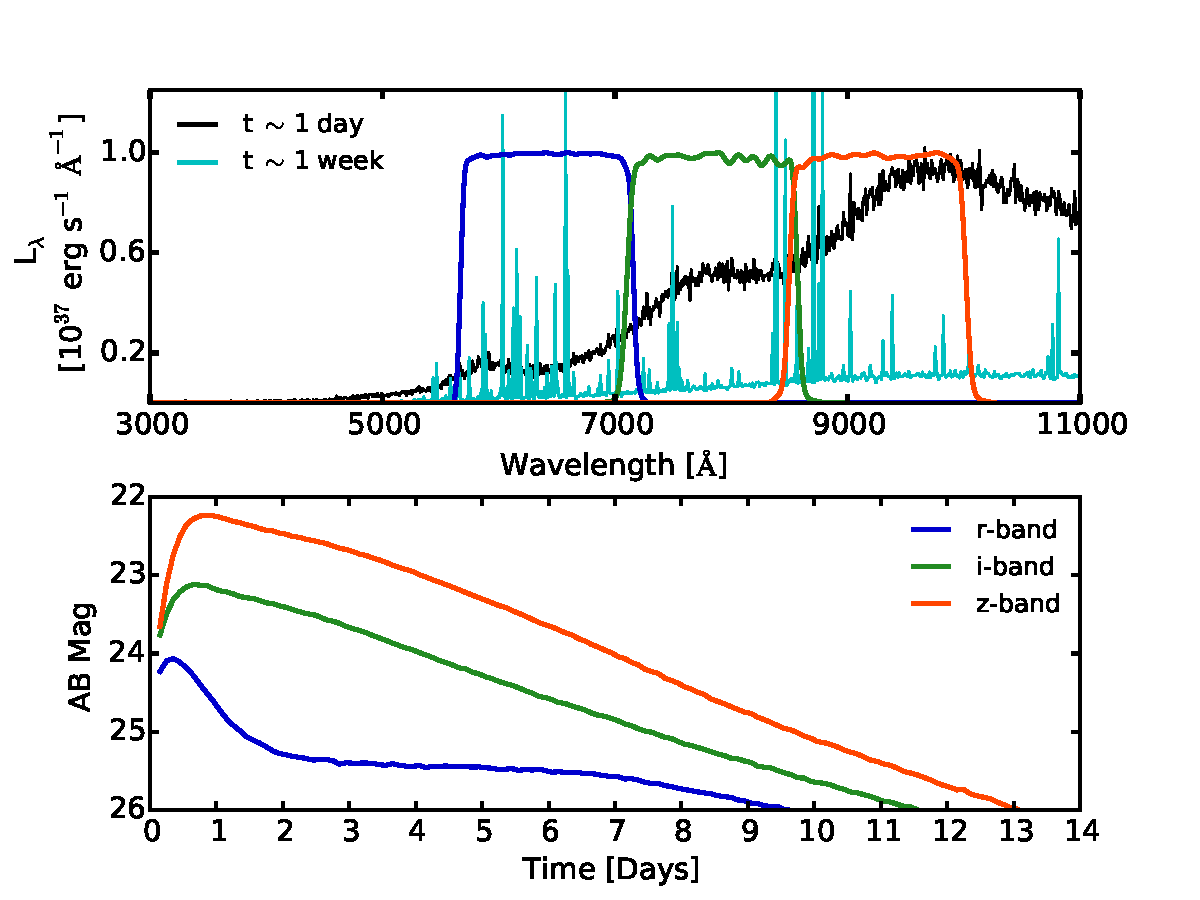
\includegraphics[width=0.9\textwidth]{./figs/chapter2/ch2_f1.pdf}
\caption{Top: Kilonova spectra from \citet{BarnesKasen13} at $\sim$ 1 d and $\sim$ 1 week with ejecta properties of $\Mej =10^{-2}\;M_{\odot}$ and $\beta_{\text{ej}} = 0.2$. Bottom: Light curve for the same model parameters computed at a fiducial distance of 200 Mpc in the DECam {\em r}, {\em i}- and {\em z}-band filters. \vspace{10pt}}
\label{fig:ch2_kilosample}
\end{figure}
   
In this work, we construct kilonova light curves using the time-resolved spectra of \citet{BarnesKasen13}. They consider a grid of models with $\Mej = 10^{-3}\;, 10^{-2} \;, \text{ and } 10^{-1} \;M_{\odot}$ and with $\beta_{\text{ej}} = $ 0.1, 0.2, and 0.3. Unless otherwise noted we only consider the average ejecta properties of $\Mej =10^{-2}\;M_{\odot}$ and $\beta_{\text{ej}} = 0.2$ since we do not know the distribution of ejecta properties a priori. We compute light curves using the DECam filter transmission curves\footnote{\url{http://www.ctio.noao.edu/noao/sites/default/files/DECam/DECam_filters_transmission.txt}}\footnote{We note that the DECam transmission filters are fairly standard so these results are relevant for other instruments as well.} with the luminosity $L_{\phi}$, through a filter $\phi$, at a time t, being given by 
\begin{align}
\label{eq:LCint}
L_{\phi}(t) = \frac{\int d\lambda L_{\lambda}(t,\lambda) \phi(\lambda)}{\int d\lambda \phi(\lambda)}
\end{align}
\noindent where $L_{\lambda}(t,\lambda)$ is the model specific luminosity and $\phi(\lambda)$ is the filter transmission as a function of wavelength. A representative plot of the spectra at 1 day and 1 week, along with the resulting {\em r}-, {\em i}-, and {\em z}-band light curves are shown in Figure~\ref{fig:ch2_kilosample}.
   
\subsection{WD-NS/WD-BH Mergers}
\label{sec:ch2_WDmerge}
The tidal disruption of a WD by a NS or BH binary companion can produce an isotropic optical transient powered by the radioactive decay of ${}^{56}$Ni synthesized in the ejecta. The ejecta have an expected mass of $\Mej \approx 0.3-1.0 \; M_{\odot}$, velocity $\vej \approx (1-5) \times 10^4$ km s$^{-1}$, and $^{56}$Ni mass of $M_{\text{$^{56}$Ni}} \approx 10^{-4.5} - 10^{-2.5}\;M_{\odot}$ \citep{Metzger2012}. These properties are primarily determined by the mass of the WD, with more massive progenitors producing higher ejecta mass, velocities, and $^{56}$Ni masses. The resulting light curves have a typical peak timescale of $t_p \sim $ week and a peak bolometric luminosity of $L_p \sim 10^{39} - 10^{41.5} \text{ erg s}^{-1}$.

The two scenarios we consider here are the merger of: (1) a $0.6\;M_{\odot}$ C--O WD with a $1.4\;M_{\odot}$ NS, and (2) a $1.2\;M_{\odot}$ O--Ne WD with a $3\;M_{\odot}$ BH. The models of \citet{Metzger2012} only include bolometric light curves. To produce {\em i}- and {\em z}-band light curves we compute an effective temperature using the \citetalias{LP98} models with $\Mej \approx 0.5\;M_{\odot},\text{ and }\vej \approx 2.8\times10^4$ km s$^{-1}$ for scenario 1, and $\Mej \approx 1\;M_{\odot},\text{ and } \vej \approx 4.6\times10^4$ km s$^{-1}$ for scenario 2 \citep[see Figure 7 of][]{Metzger2012}. We integrate the resulting blackbody curve over the DECam filters using Equation~\ref{eq:LCint} and compare to the bolometric luminosity to generate bolometric corrections. For the WD-NS merger, we find $T_p \approx 6000$ K leading to $m_{\text{bol}} - m_{\text{i}} \approx -1.9$ mag and $m_{\text{bol}} - m_{\text{z}} \approx -2.2$ mag. The WD-BH merger calculation yields $T_p \approx 7850$ K leading to $m_{\text{bol}} - m_{\text{i}} \approx -2.2$ mag and $m_{\text{bol}} - m_{\text{z}} \approx -2.6$ mag. We assume that these corrections are constant in time. The bolometric corrections are applied to the light curves of \citet{Metzger2012} to generate the light curves used in this analysis (see Figure~\ref{fig:ch2_LCcont}).

\subsection{White Dwarf Accretion Induced Collapse}
\label{sec:AIC}
The accretion of material onto an O--Ne WD near the Chandrasekhar mass can cause the degenerate star to undergo electron capture in its interior resulting in the formation of a NS, rather than a thermonuclear explosion. This process is known as accretion induced collapse (AIC). If the WD is rapidly rotating then a stable accretion disk will form. The disk will cool and become radiatively inefficient, driving powerful outflows with a characteristic ejecta mass of $\Mej \sim 10^{-2}\;M_{\odot}$ and velocity $\beta_{\text{ej}} \sim 0.1$. The outflowing material has an electron fraction of $Y_e \sim 0.5$ due to neutrino radiation from the proto-NS and synthesizes $\text{a few} \times 10^{-3}\; M_{\odot}$ of ${}^{56}$Ni powering an optical transient \citep{Metzger+09b}. Radiative transfer calculations by \citet{Darbha+10}, motivated by the models of \citet{Metzger+09b}, provided light curves of AIC events. They found that the resulting transient is rapidly evolving with the light curve peaking at $t_p \sim$ 1 day with a bolometric luminosity of $L_p \sim 2\times10^{41}$ erg s$^{-1}$.

We use the models of \citet{Dabhra+10} to compute \emph{i} and \emph{z}-band light curves using the same methodology as in Section~\ref{sec:ch2_WDmerge}. The effective blackbody temperature has an assumed fiducial value of $T_p \approx 5800$ K from the models of \citet[see their Figure 3]{Dabhra+10}. The resulting bolometric corrections are therefore $m_{\text{bol}} - m_{\text{i}} \approx -1.9$ mag and $m_{\text{bol}} - m_{\text{z}} \approx -2.2$ mag. We assume that these corrections are constant in time and apply them to the bolometric light curves to generate $i$- and $z$-band light curves (Figure 2).

\subsection{White Dwarf Double Detonation}
\label{sec:ch2_ELDD}
Detonation of a sufficiently large accreted He envelope $(M_{\text{He}} \sim 0.2\; M_{\odot})$ on the surface of a C--O WD can generate shock waves which then propagate to the core leading to the total detonation of the WD. In simulations performed by \citet{Sim+12}, two possible detonation scenarios were considered. The first, edge-lit double detonation (ELDD), occurs when the initial detonation takes place at the surface of the WD. This produces a transient that is expected to reach a peak bolometric luminosity of $L_p \sim 10^{42}$ erg s$^{-1}$ at $t_p \sim 8$ d. The second scenario is the compression-shock double detonation (CSDD), where the core is compressed by the shock wave and C--O detonation occurs closer to the center of the WD. The transient is brighter than in the ELDD scenario with a peak bolometric luminosity of $L _p \sim 4\times10^{42}$ erg s$^{-1}$, and a correspondingly longer rise time ($t_p  \gtrsim 10$ d). In the CSDD scenario the transient is also longer-lived with no significant decline in brightness for $\sim 30$ d.

The slow evolution of the CSDD model light curve relative to kilonovae means that it can be easily removed from consideration as a contaminant on the basis of timescales alone. However, we still consider the ELDD scenario as the more rapid rise time and comparably faster decline means that it could serve as a potential contaminant. We make use of bolometric light curves from the simulations of \citet{Sim+12} to compute DECam {\em i}- and {\em z}-band light curves as in Section~\ref{sec:ch2_WDmerge}. The ELDD spectrum is approximated as a blackbody with a characteristic temperature of $T_p \approx 4800$ K using the model spectra of \citet[see their Figure 7]{Sim+12}. The bolometric corrections are found to be $m_{\text{bol}} - m_{\text{i}} \approx -1.7$  mag and $m_{\text{bol}} - m_{\text{z}} \approx -1.9$ mag. We assume that these corrections are constant in time and apply them to the bolometric light curves to generate $i$- and $z$-band light curves (Figure 2).

\subsection{Type .Ia Supernovae}
\label{sec:ch2_type.Ia}
Another possible WD-based transient is the detonation of an outer shell of helium on the surface of the WD. This can occur when the mass accretion rate from the donor is low enough that burning in the He shell becomes thermally unstable. The specific term ``type .Ia" was coined as a reference to He detonation in an AM Canum Venaticorum system (AM CVns) where the donor star is degenerate or semi-degenerate and accreting He rich material onto a C--O or O--Ne WD \citet{Bildsten+07,Shen+10}. The typical envelope mass is $M_{\text{env}} \sim \text{few}\times10^{-2}-10^{-1}\;M_{\odot}$ and the detonation ejects the bulk of the envelope at a typical velocity of $\vej \sim 10^4$ km s$^{-1}$. This leads to a transient with a typical peak time of $t_p \sim 2-10$ d and a peak bolometric luminosity of $L_p \sim 5\times10^{41} - 5\times 10^{42}$ erg s$^{-1}$ \citep{Shen+10}.

We produce type .Ia light curves from the time-resolved spectra computed from the models of \citet{Shen+10}. We consider the models $0.6+0.2\;M_{\odot}$, $0.6+0.3\;M_{\odot}$, $1.0+0.05\;M_{\odot}$, and $1.2+0.05\;M_{\odot}$, where the first number is the WD mass and the second number is the mass of the He envelope. We integrate the spectra over the DECam filter transmission curves as described in Section~\ref{sec:ch2_kilo} (Figure~\ref{fig:ch2_LCcont}).

\subsection{Pan-STARRS Fast Transients}
\label{sec:ch2_PSFast}
\citet{Drout+14} discovered ten rapidly evolving transients in the Pan-STARRS1 Medium Deep Survey. These events are characterized by a time above half-maximum of less than 12 days and have typical absolute magnitudes of $M \approx -16.5 \text{ to } -20$ mag. These objects have blue colors with {\em g} $-$ {\em r} $\lesssim$ --0.2 at peak \citep{Drout+14}. While the existing sample is small these events may end up being a significant contaminant in the fast cadence, wide-field GW searches investigated here. Therefore, we consider the {\em i}- and {\em z}-band light curves of three objects from \citet{Drout+14}: PS1-10ah, PS1-10bjp, and PS1-11qr. They possess sufficient pre-peak data for our analysis while providing a representative range of timescales and luminosities for the sample (Figure~\ref{fig:ch2_LCcont}).
   
\subsection{Type Ia Supernovae}
\label{sec:ch2_typeIa}
Type Ia supernova result from the thermonuclear explosion of a C--O WD. While these SNe have timescales much longer than those of kilonovae and other transients considered in this section, their high volumetric rate and large luminosity mean that a deep optical search for kilonovae will detect large numbers of Type Ia SNe. This makes them a particularly likely contaminant in such searches. We focus our analysis on the event SN2011fe discovered in M101 by the Palomar Transit Factory \citep{Nugent+11a} due to the high quality of available data. In addition to being one of the closest known Type Ia SNe \citep[$\mu = 29.04\pm0.19$,][]{ShappeeStanek11}, SN2011fe was discovered a mere 12 hours after explosion \citep{Nugent+11b} leading to coverage starting at --15 days relative to the {\em B}-band peak (R). In this work, we use the 32 spectral observations compiled by \citet{Pereira+13} to produce DECam {\em i}- and {\em z}-band light curves as a function of redshift, including K-corrections, using the process described in Section~\ref{sec:ch2_kilo} (Figure~\ref{fig:ch2_LCcont}).

\begin{figure}[h!]
\centering
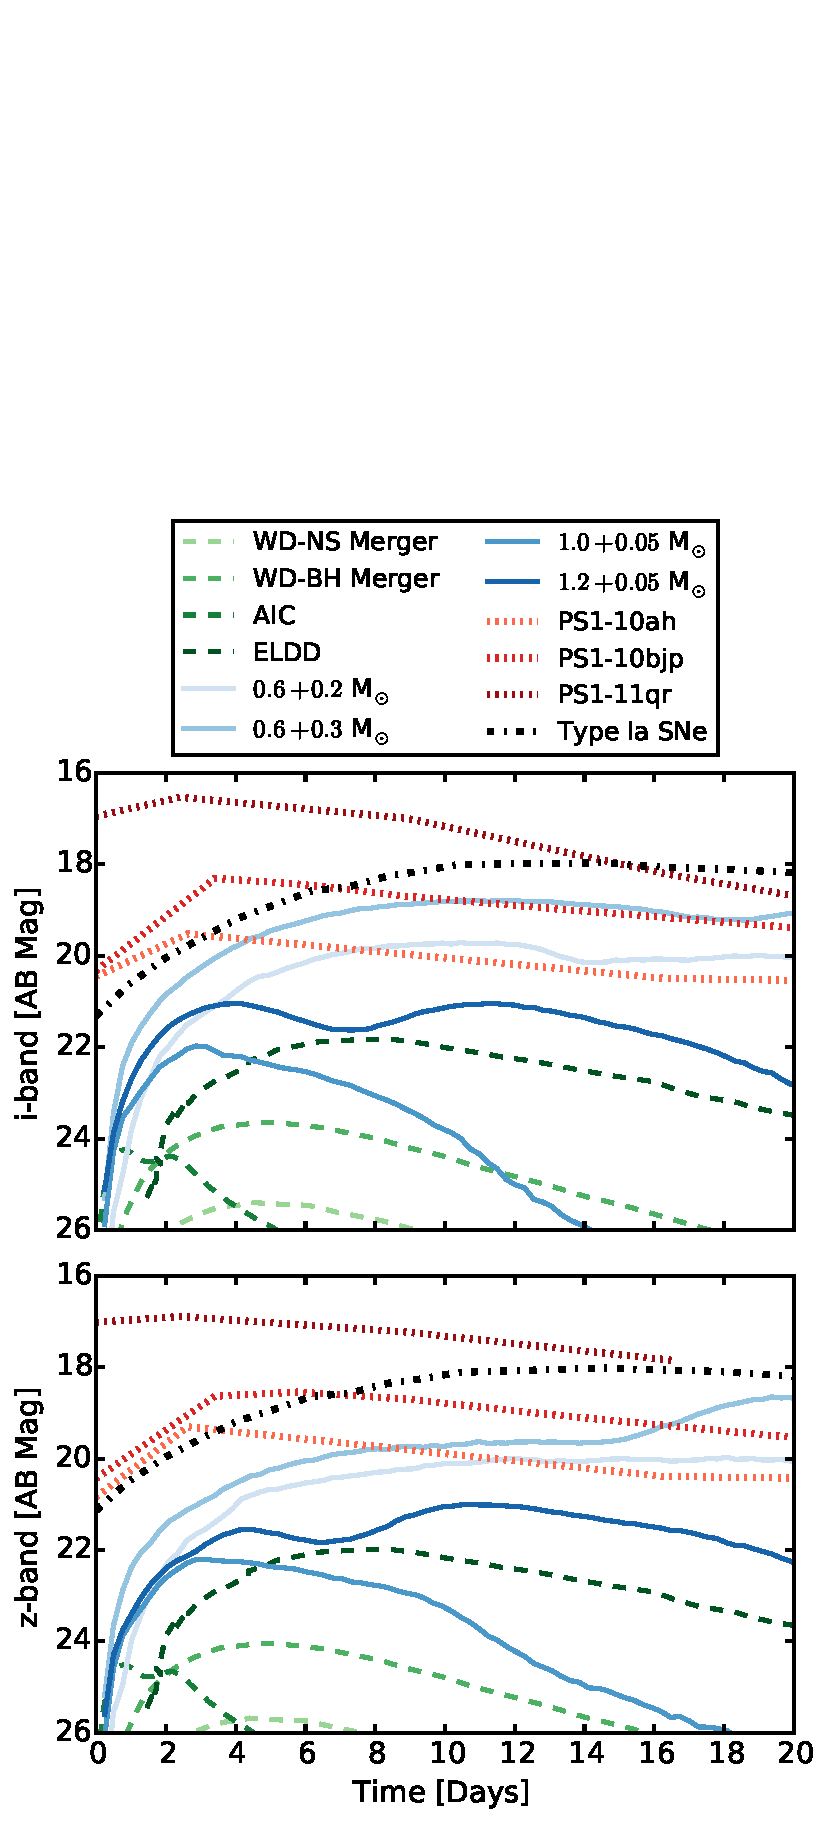
\includegraphics[trim= 0 0 0 240 ,clip,width=0.6\textwidth]{./figs/chapter2/ch2_f2.pdf}
\caption{Top: {\em i}-band light curves of the contaminants considered in this work at a fiducial distance of 200 Mpc. Bottom: {\em z}-band light curves. See Sections~\ref{sec:ch2_WDmerge}~--~\ref{sec:ch2_typeIa} for details.}
\label{fig:ch2_LCcont}
\end{figure}
   
\subsection{Stellar Flares}
\label{sec:ch2_flarestar}
Stellar flares, primarily from M dwarfs, are another potential contaminant in fast cadence wide-field optical searches \citep{Becker+04,KulkarniRau06,Berger+13}.  These flares have characteristic timescales of minutes to hours \citep[see e.g.,][]{Berger+13} and temperature of $T_p \sim 10^4$ K, leading to an appearance as fast and blue transients.  As a result, M dwarf flares will only appear as a significant contaminant in kilonova searches that rely on single-epoch detection, primarily in $g$- and $r$-band in which the kilonova timescale is shorter than in the redder bands.  We return to this point in Section~\ref{sec:ch2_disc}.  The sky-projected M dwarf flare rate at the depths relevant for kilonova searches is large, $\sim 10$ deg$^{-2}$ day$^{-1}$ \citep{KulkarniRau06}.  On the other hand, as was demonstrated by \citet{Berger+13}, deep observations in the $i$- and $z$-band can easily reveal the underlying M dwarfs and hence reduce the potential for contamination from flares.

\subsection{AGN Variability}
\label{sec:ch2_agns}
We also consider short-duration optical variability from active galactic nuclei (AGNs). AGN typically show strong variability on month or year-long timescales, making AGN outbursts too long in duration to be confused with a kilonovae. However, recent work has detected rare cases of day-long  or shorter variability in the NIR. \citet{Genzel+03} observed an H-band flare in Sgr A$^{*}$ during which the source brightened by a factor of 5. This flare lasted $\sim$ 30 min, with a characteristic rise time of $\sim2-5$ min. Such short timescale flares can be ruled out as kilonova contaminants by requiring a detection on more than a single night. Flares with longer durations are also unlikely to be significant contaminants. \citet{Totani+05} performed {\em V}- and {\em i}-band observations of six AGN, selected on the basis of their variability, over a period of four days. They found typical variability of only $\sim1-5\%$ above their host galaxy luminosity. More recent work by \citet{Ruan+012} studied the variability of a sample of \fermi selected blazars. They found that these sources showed a typical rms variability of $\sim0.6$ mag on timescales of $\sim 10$ d. Therefore, AGN are unlikely to exhibit sufficiently large variability to be confused with a kilonova.
   
\subsection{Volumetric Rates}
\label{sec:ch2_rates}
An additional important factor for understanding the impact of potential contaminants on fast cadence, wide-field searches is their volumetric rates. We note that the rates for these types of objects are generally poorly understood due to the lack of strong observational constraints; the notable exception are Type Ia SNe. The volumetric rates of potential contaminants are compiled in Table~\ref{tab:ch2_rates}. No values are provided in the literature for the ELDD volumetric rate so we assign a fiducial value of 1\% of the Type Ia SN rate, consistent with the other rapid transients in this study. The volumetric rate for Type Ia SNe is known to be a function of redshift, and we use an approximate average volumetric rate in redshift bins of $\Delta z \sim 0.25$ out to $z_{\text{max}} \sim 0.75$. \citep[][and references therein]{Li+11,Graur+14}. These rates are listed in Table~\ref{tab:ch2_rates_Iae}.

To estimate the expected number of events observed during a GW optical follow-up search we compute the number of sources per square degree per year. This is done by determining the maximum redshift to which the object can be observed to a limiting magnitude of $z \approx$ 23 mag (see Sections~\ref{sec:ch2_kilo} and~\ref{sec:ch2_MCsims_det}). This rate is then multiplied by the search area $(A \sim 100$ deg$^2$) and duration to get the number of expected sources for our observations. We compute the duration by assuming that a kilonova will be detected within approximately one day of the GW trigger. Therefore, we do not consider events that begin more than +2 d into the search. However, we do consider sources that begin up to twice their characteristic timescale ($\sim5$ d for rapid transients and $\sim 20$ d for Type Ia SNe) prior to the GW trigger, as they may remain visible when the search begins. The total duration is then 7 d for rapid transients and 22 d for Type Ia SNe. The number of expected sources is given in Tables~\ref{tab:ch2_rates} and~\ref{tab:ch2_rates_Iae}. Type Ia SNe dominate the number of expected events with $N \sim 568$ when summing across all redshift bins. Of the population of fast transients, only type .Ia and the Pan-STARRS fast transients are expected to have $N \gtrsim 1$. Despite the low expected occurrence rate for other fast transients, we still consider these sources in this analysis due to the large uncertainty in their rates.

\section{The Color-Magnitude-Timescale Phase-Space}
\label{sec:ch2_phase}      
In this section we assess the possibility that any of the potential contaminants discussed in Section~\ref{sec:ch2_contaminants} could be confused  for a kilonova during a GW follow-up observation. We consider the maximum detection distance for a NS-NS binary merger to be 200 Mpc ({\em z} $\approx$ 0.05), while for the contaminating sources we utilize larger distances as appropriate. We establish a three-dimensional phase-space based on the peak {\em z}-band brightness, the {\em i} $-$ {\em z} color at {\em z}-band peak, and the rise time, defined as the time it takes the transient to rise one magnitude to peak in {\em z}-band. We compute the phase-space coordinates at 200 Mpc for all of the transients discussed in Section~\ref{sec:ch2_contaminants}. We then examine all of the potential contaminants at {\em z} $\sim$ 0.2, 0.4, and 0.6. In cases where time resolved spectra were available, the spectra were appropriately redshift-corrected in both time and wavelength. Sources modeled with a blackbody function had redshift corrections applied to the effective temperature. The rise time-color slice of this phase-space is shown in the left column of Figure~\ref{fig:ch2_phase} while the rise time-magnitude slice is shown in the right column of Figure~\ref{fig:ch2_phase}.
   
\begin{figure*}[t!]
\centering
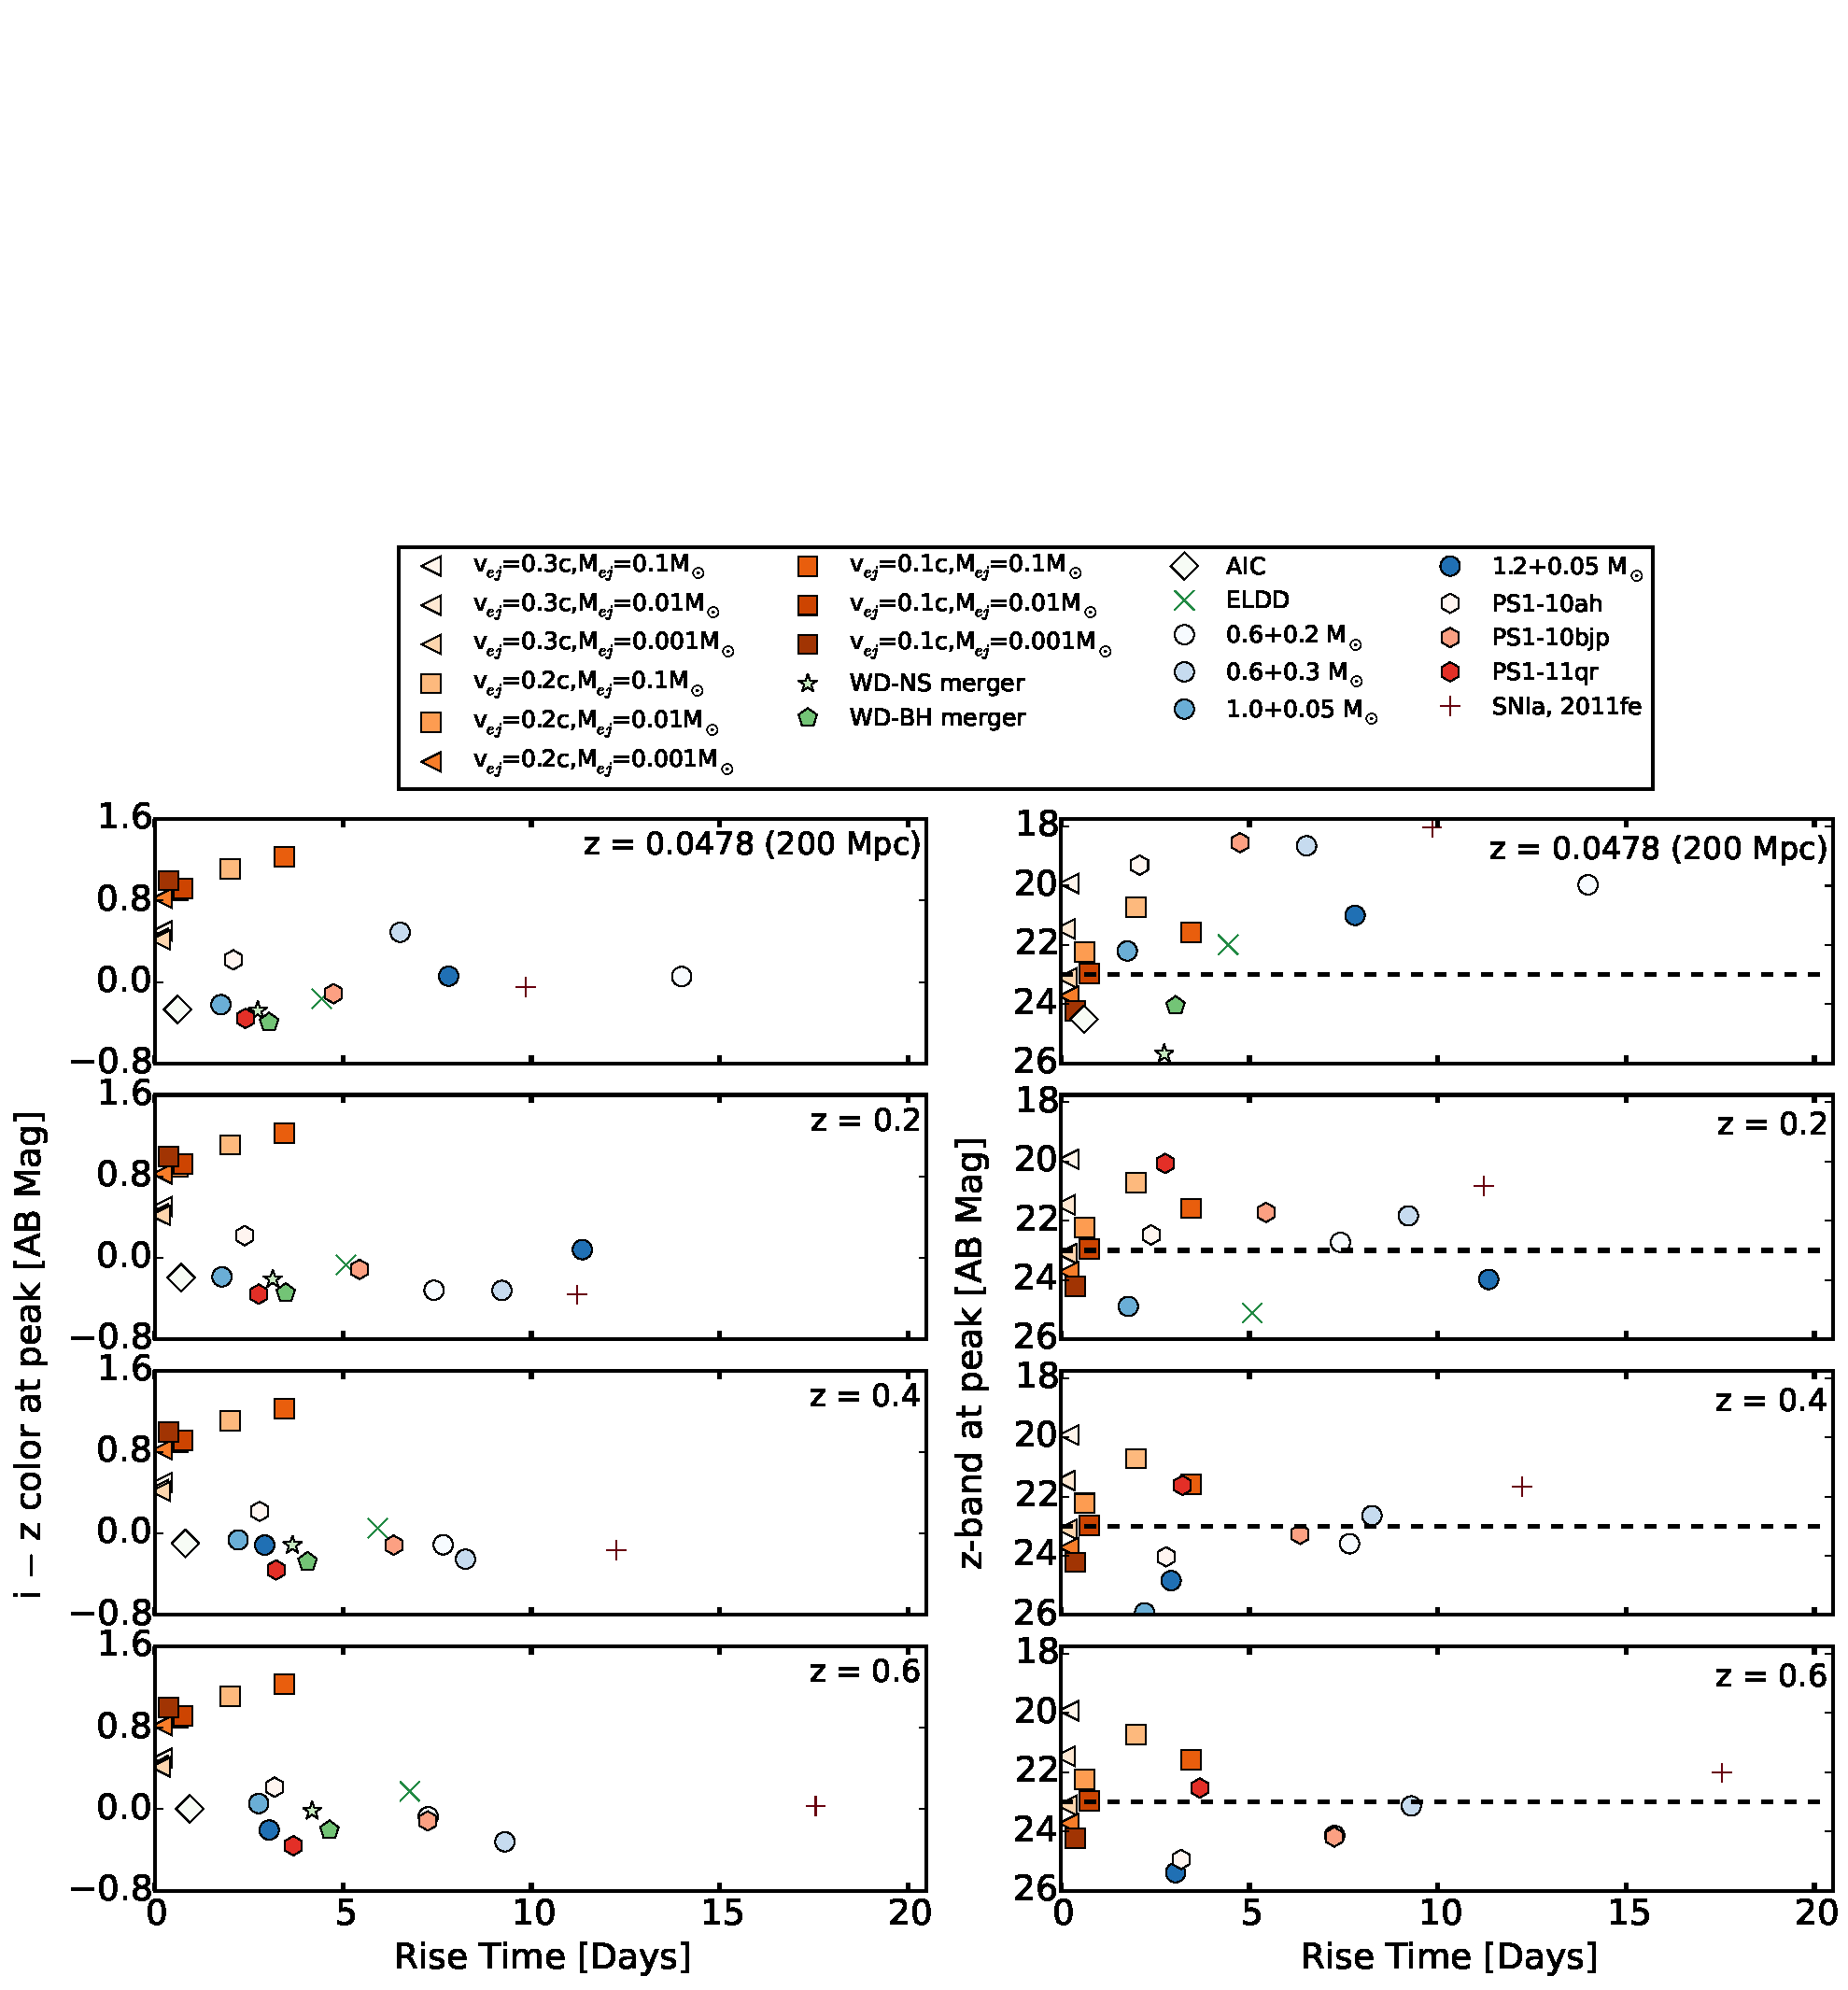
\includegraphics[trim= 0 0 0 250 ,clip,width=\textwidth]{./figs/chapter2/ch2_f3.pdf}
\caption{Time-color (left) and time-magnitude (right) slices of the time-color-magnitude phase-space at a selection of redshifts. Arrow markers denote upper limits on the rise time. Note that in all panels the population of kilonovae are kept at the fiducial distance of $\sim$ 200 Mpc while redshift corrections are applied to the contaminant population. Kilonovae are well separated from the contaminant population in both color and timescales. The delineation in magnitude is less apparent.}
\label{fig:ch2_phase}
\end{figure*}
   
Investigating the first panel in the rise time-color space, we can see that the nine kilonovae models are well separated from the population of contaminating sources by virtue of their redder color. We also note that their rise times are generally shorter, with only the AIC and $1.0+0.05\;M_{\odot}$ type .Ia light curves exhibiting comparable timescales. The region occupied by kilonovae in the rise time-peak brightness phase-space is not as tightly constrained. They are still well separated by timescale but several of the contaminating sources have comparable peak brightnesses at 200 Mpc. As we consider more distant contaminant populations, we observe little to moderate reddening, with all of the contaminants remaining blue compared to the kilonovae population ($i-z\lesssim$ 0 mag to {\em z} $\sim$ 0.6). The $0.6+0.3\;M_{\odot}$ and $1.2+0.05\;M_{\odot}$ Type .Ia SNe models have $i-z\sim$ 0.2 mag, but their longer timescales $(t\sim\text{ week})$ keep them well separated from kilonovae. In addition, there is a systematic change in timescales, with all of the contaminants (except for the AIC events) shifting to a rise time of $\gtrsim  2$ d by {\em z} $\sim$ 0.6 due to time dilation. 
   
The inherent low luminosity of most fast transients means that they quickly drop below the sensitivity limit of a reasonable search (e.g., $m_z \approx 23$ AB mag). Only the Type Ia SNe, Pan-STARRS fast transients, and the most luminous type .Ia models are brighter than $\approx$ 23 AB mag by {\em z} $\sim$ 0.2, and by {\em z} $\sim$ 0.6 only the transient PS1-11qr and Type Ia SNe will still be detectable. 

Quantitatively, we can impose cuts of $t_{\text{rise}} \lesssim  5$ d, $i-z \gtrsim 0$ mag, and $m_z \lesssim 23$ mag to isolate kilonovae from contaminants. For sources at $z \lesssim 0.2$, this will isolate kilonovae from all contaminants except the Pan-STARRS fast transient PS1-10ah. These cuts remain effective for more distant sources as well. For example, at $z\sim0.6$, AIC, the $0.6+0.3\;M_{\odot}$ Type .Ia SNe, and PS1-10ah all exhibit $t_{\text{rise}} \lesssim  5$ d and $i-z \gtrsim 0$ mag. However, they no longer pass the brightness cut, with $m_z \gtrsim 23$ mag. Therefore, we conclude that given well-sampled light curves, we can use the rise time-color-brightness phase-space to separate kilonovae from the contaminant population of other rapidly evolving sources.
 
\section{Simulated Follow-Up Observations}
\label{sec:ch2_MCsims}
The analysis in the previous section was based on the idea that it is possible to obtain well-sampled light curves of kilonovae and other fast transients, but in reality the search cadence for a large area and the required depth will lead to at most a few light curve points. To explore the impact of realistic observations we utilize Monte Carlo (MC) simulations which model a set of GW follow-up observations parameterized by cadence, limiting magnitude, and start time following a GW trigger.  The goal of these simulations is two-fold. First, we study the feasibility of extracting useful light curve parameters for the kilonovae. This includes the actual detection of a kilonova, as well as its detection on the rise, which is important for establishing the ejecta parameters. Second, we study the impact of the contaminant population on our ability to identify kilonovae by utilizing our simulated observations to explore the rise time-color-magnitude phase-space established in Section~\ref{sec:ch2_phase}.

The detection of transient sources in wide fields necessitates difference imaging. In the simplest scenario a pre-existing image of the field can be used as a template to eliminate the non-varying sources. In the context of real-time GW follow-up, however, such template images may not be available until after the source fades away. To address this difficulty, we consider three scenarios:
\begin{enumerate}
\item The GW event is localized to a region with pre-existing template images. For example, the event occurs in a region previously observed to a similar or greater depth by the wide-field telescope being used for the follow-up.
\item Template images are obtained after the source has faded. For kilonovae follow-up, this requires observations at $\gtrsim10$ days after the GW trigger.
\item The first observation taken as part of a GW follow-up campaign is used as the template image.
\end{enumerate}

From an analysis standpoint, the first two scenarios are identical as both involve a template image which contains no flux from the transient source. This allows robust subtractions to be performed, as well as precise measurements of brightness and color. However, the second scenario does not allow for the real-time identification of the transient, which is critical for obtaining follow-up spectroscopy and NIR imaging. These scenarios are the primary focus of this section. 

The third scenario, using the first observation as a template, is more challenging. The potential for the presence of flux from the transient in the template image means that we can only measure a relative difference in brightness. When this difference is small compared to the noise in the image it becomes difficult to measure key quantities such as color or even claim that the source has been detected in difference imaging. We note that the second and third scenarios are not mutually exclusive. If the kilonova can not be identified in real-time under the third scenario, then a template image can still be obtained after the source has faded away and scenario 2 becomes applicable. These issues are addressed in Section~\ref{sec:ch2_diff}.

\subsection{Detectability of Kilonovae in Simulated Observations}
\label{sec:ch2_MCsims_det}
We first investigate the issue of kilonova detectability, as well as observation of the light curve during the rise to peak brightness. We explore four observing strategies utilizing $\sim$1 week of observations in both {\em i}- and {\em z}-band with the following cadences:
{\small \begin{enumerate}[leftmargin = 2.5cm]
\item[Strategy 1:] One visit per night for the duration of the search (i.e., N1, N2, N3, N4, N5, N6). 
\item[Strategy 2:]  One visit per night on the first two nights, followed by a visit every other night (i.e., N1, N2, N4, N6).
\item[Strategy 3:]  Two visits $\sim$ 3 hr apart on the first night, followed by one visit per night for the duration of the search (i.e., N1, N1, N2, N3, N4, N5, N6). 
\item[Strategy 4:]  Two visits $\sim$ 3 hr apart on the first night, followed by a visit every other night (i.e., N1, N1, N3, N5)
\end{enumerate}}
\noindent These strategies are chosen to probe a range of timescales while representing differing levels of time investment, and possible loss of coverage due to adverse weather during follow-up observations. 
   
For each observing strategy we establish a grid of start times following a GW trigger and a $5\sigma$ limiting magnitude. The range of grid values is $t_{\text{start}} = 3-24$ hr in steps of 3 hr and $m_{\text{lim}} = 21-27$ AB mag in steps of 1 AB mag. The range of start times represents the fact that a GW trigger may occur when the source is not readily visible in the night sky, while the range of limiting magnitudes covers the depths achievable by current and future wide-field instruments. At each point on this grid we conduct 50,000 simulated observations, with an observation being comprised of: (1) a kilonova with $M_{\text{ej}} = 10^{-2} \text{ M}_{\odot}$ and $\beta_{\text{ej}} = 0.2$ placed at a distance of up to 200 Mpc using a uniform volume distribution; (2) the light curve of the kilonova is computed for the chosen distance using the methodology outlined in Section~\ref{sec:ch2_kilo}; (3) the observation times are computed based on the chosen strategy; for example if the start time is 12 hours and strategy 1 is chosen, then observations will be conducted at 0.5 d, 1.5 d, 2.5 d, and so on; and (4) the source flux in $riz$-bands DECam filters is measured at the selected times using the light curves computed in step (2). If the kilonova brightness exceeds the search depth in at least three epochs, the event is flagged as a detection. If there is an observed increase in brightness between two epochs, the event is also flagged as ``rising."
 
\begin{figure}[t!]
\centering
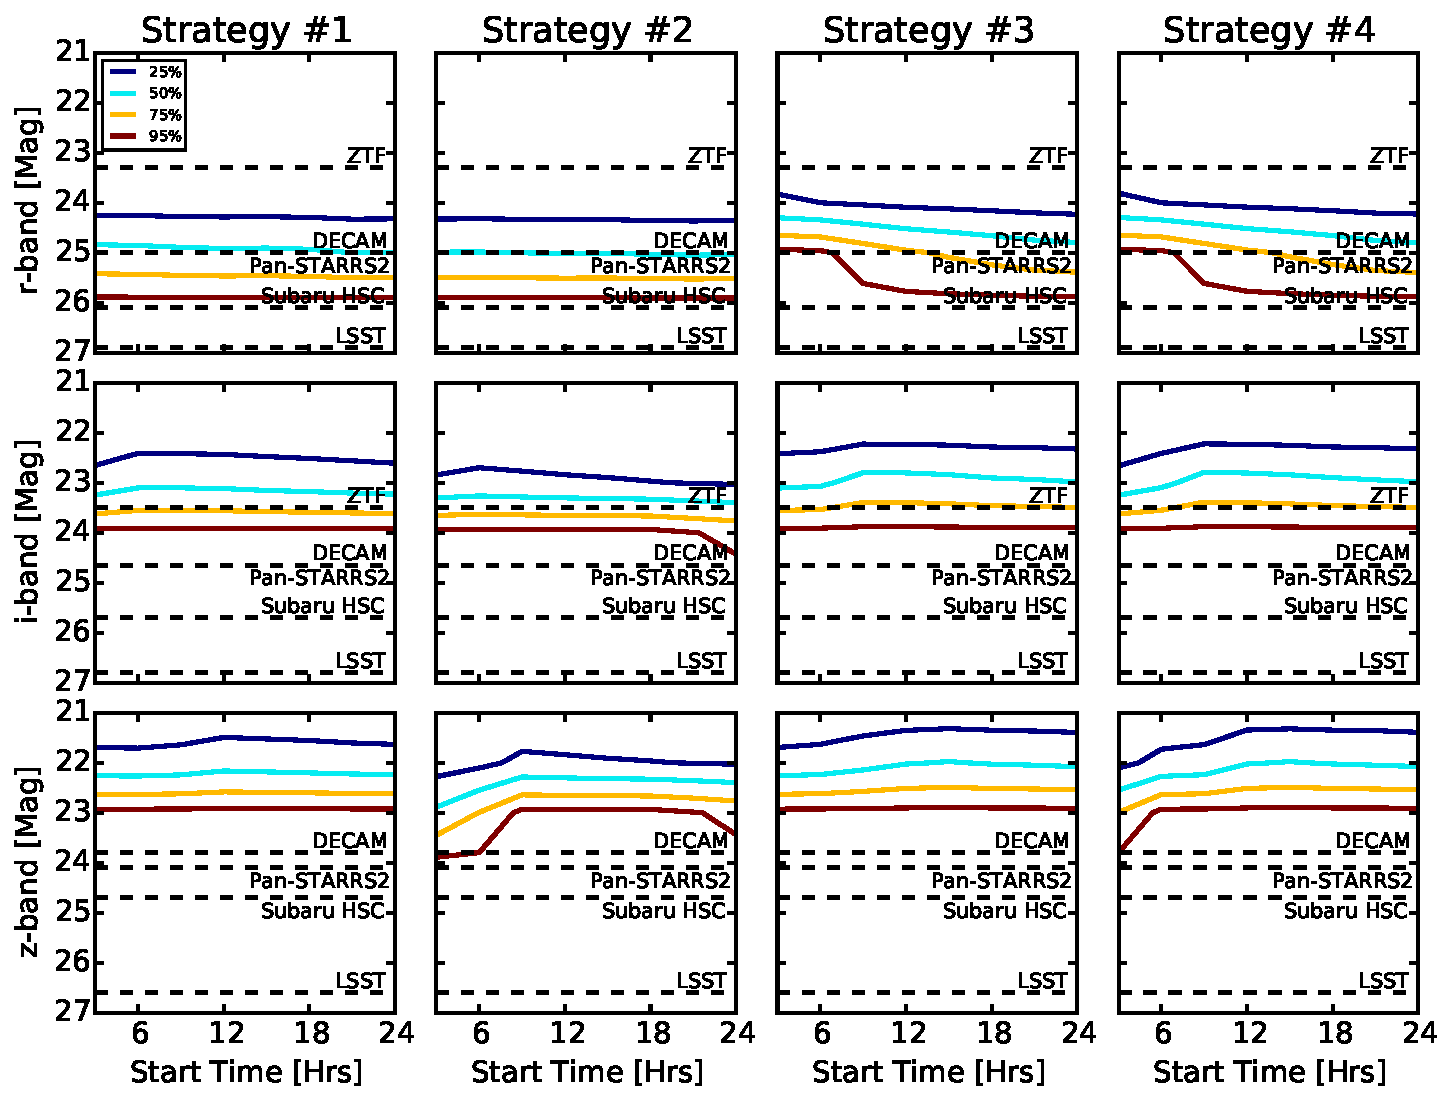
\includegraphics[width=0.9\textwidth]{./figs/chapter2/ch2_f4.pdf}
\caption{Depth versus start time grid in $r$ (top), $i$ (middle), and $z$ (bottom) for the four observing strategies. The contours indicate the fraction of sources detected in at least three epochs (25\% blue, 50\% cyan, 75\% yellow, 95\% red). The dashed lines represent the approximate 5$\sigma$ limiting magnitudes of several wide-field telescopes assuming the appropriate number of pointings necessary to cover a $\sim 100$ deg$^2$ error region with the required cadence. The choice of observing strategy does not drastically affect the fraction of sources detected at a given depth. We note that the early time drop in efficiency for {\em z}-band utilizing Strategy 2 is the result of the initial observations occurring before the light curve has brightened above the limiting magnitude.}
\label{fig:ch2_det}
\end{figure}
   
In Figure~\ref{fig:ch2_det} we plot contours of the fraction of events detected for each of the four observing strategies in the $riz$-bands, as a function of survey depth and start time. The dashed lines represent the approximate 5$\sigma$ limiting magnitudes of several wide-field telescopes assuming the appropriate number of pointings necessary to cover a $\sim 100$ deg$^2$ error region with the required cadence.
   
We find that the choice of observing strategy does not strongly impact the fraction of sources detected at a given depth. In particular, in {\em r}-band (Figure~\ref{fig:ch2_det}, top row) we find that for both Strategies 1 and 2, the typical depth required to detect 50\% of events is $\approx25$ mag, while a depth of $\approx26$ mag is required to detect 95\% of events. This challenge is slightly alleviated by Strategies 3 and 4, which involve two observations on the first night. In this case, an early start time $(\lesssim 6$ hr) allows 50\% (95\%) of events to be detected at a depth of $\approx24.3\,(25)$ mag. Consequently only Subaru HSC and LSST will be able to achieve the required depth for routine detections in $r$-band. The redder bands offer more favorable conditions, with the {\em i}-band 50\%(95\%) detection rate achieved at a depth of $\approx 23(24)$ mag across all four strategies. Lastly, we find that the {\em z}-band contours indicate that a depth of $\approx22.2\,(23)$ mag is required to achieve a 50\% (95\%) detection rate across all four strategies. In these cases, DECam, Pan-STARRS2, and Subaru HSC can all achieve the required depths for routine detections in $i$- and $z$-bands.  These values are summarized in Table~\ref{tab:ch2_det}.

We also find that for {\em z}-band the observing strategies utilizing longer cadences (i.e., Strategies 2 and 4) produce a noticeable drop in efficiency if the first observation occurs too early ($\lesssim 6$ hr). In this case, the light curve has not yet brightened above the survey depth, causing the initial observation to be a non-detection. The slow cadence after the initial night of observations (at $\gtrsim2$ days) is then insufficient to capture the requisite three detections before the light curve fades below the detection limit. Quantitatively, we find a loss of $\sim 1$ mag for Strategies 2 and 4 for starting times $\lesssim 6$ hr. This indicates that the strategies involving slower cadence after the initial night of observations are not well matched to kilonova timescales. 

\begin{figure}[t!]
\centering
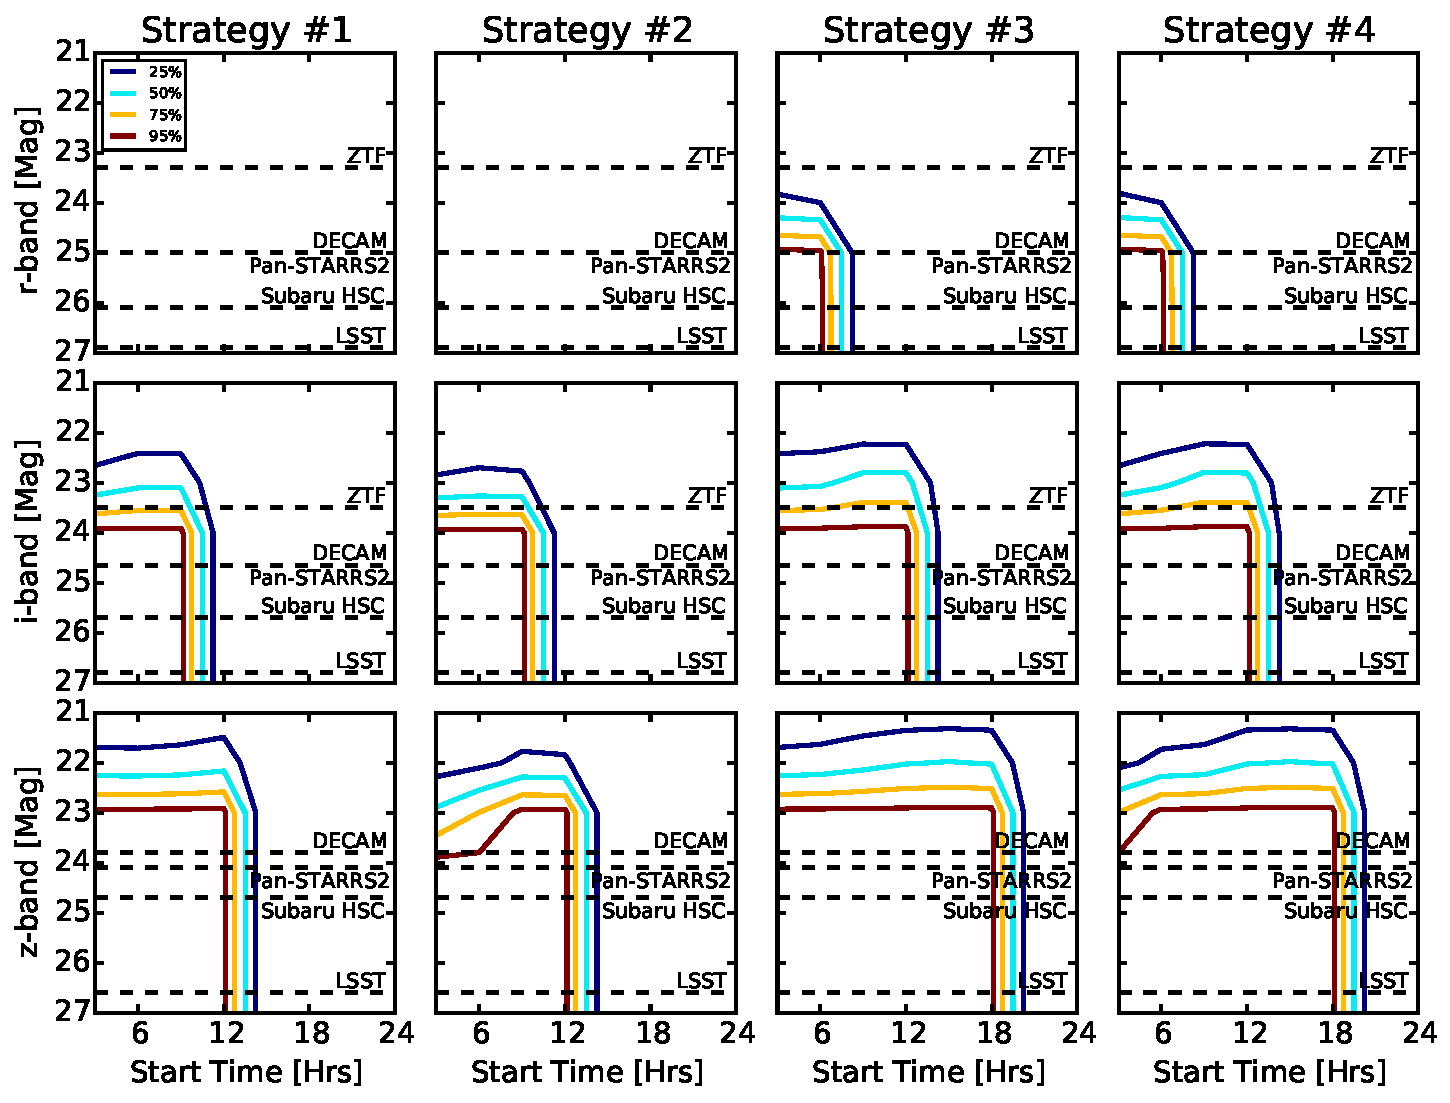
\includegraphics[width=0.9\textwidth]{./figs/chapter2/ch2_f5.pdf}
\caption{Same as Figure~\ref{fig:ch2_det}, except that the contours show the fraction of events for which a brightening is detected. The choice of observing strategy, start time, and filter have a strong impact on the detection of brightening.}
\label{fig:ch2_rise}
\end{figure}
   
While the particular choice of search strategy does not strongly impact the detection fraction at a given survey depth, the choice of strategy is important when trying to detect the {\em brightening} of a kilonova. We investigate this point in Figure~\ref{fig:ch2_rise}, which shows contours for the fraction of events that are seen to brighten between any two epochs. These events must also meet the detection criterion utilized in Figure~\ref{fig:ch2_det}. As in Figure~\ref{fig:ch2_det}, the contours are plotted as a function of start time and search depth for each of the observing strategies and filters. In {\em r}-band, utilizing Strategies 1 and 2, a brightening phase is not detected even to a limiting magnitude of 27 mag. This is because the {\em r}-band light curve peaks in $\lesssim 1$ day (Figure~\ref{fig:ch2_kilosample}) necessitating a rapid early time cadence to capture the event as it brightens. For Strategies 3 and 4, with two observations on the first night, brightening can be observed for 50\% (95\%) of events provided the observations reach a limiting magnitude of $\approx24.3\,(25)$ mag and begin within 8 (6) hr of the GW trigger.
   
The detection of the light curve rise is more favorable in {\em i}- and {\em z}-band. In general, the contours shown in Figure~\ref{fig:ch2_rise} are identical to those in Figure~\ref{fig:ch2_det}, but truncated as the start time becomes comparable to the peak time of the light curve. Therefore, brightening can be detected provided observations begin early enough and assuming the required depth is achieved. For {\em i}-band, with Strategies 1 and 2, we find that observations starting within 6 (8) hr of the GW trigger can detect brightening in 50\% (95\%) of events. With Strategies 3 and 4 the required start time for a detection rate of 50\% (95\%) extends out to 12 (14) hr. In {\em z}-band the observations can achieve detection rates of 50\% (95\%) provided they begin within 12 (15) hr of the GW trigger. The starting time can be extended to 18 (21) hr when Strategies 3 and 4 are utilized. We also note that Strategies 2 and 4 show the same early time ($\lesssim 6$ hr) loss of $\sim$ 1 mag as seen in Figure~\ref{fig:ch2_det}. The broader range of starting time allowed by strategies 3 and 4 highlight the advantage of rapid follow-up of GW triggers. However, these initial simulations consider any observed brightening as the detection of a rise. It may be the case that the actual change in brightness is not statistically significant, making a robust detection of a rise impossible. 
    
We investigate the actual change in brightness relative to the instrument sensitivity using a modified version of our initial simulations. We no longer operate on the depth-start time grid, but instead consider a fiducial fixed depth of 24 AB mag in {\em r}- and {\em i}-band and 23 AB mag in {\em z}-band (as appropriate for achieving an acceptable detection fraction). The start time is randomly selected using a uniform distribution ranging from 3 to 24 hr. The same four observing strategies are employed and we run 50,000 iterations per strategy, utilizing the same procedure as before. We then compute the change in magnitude between the first two epochs ($\Delta m_{21} \equiv m_2 - m_1$), and between the first and third epochs ($\Delta m_{31} \equiv m_3 - m_1$). We employ the same detection criteria as in the previous simulations, requiring the source to be detected in at least three epochs. We consider sources that are observed to either rise or decline.
   
\begin{figure}[t!]
\centering
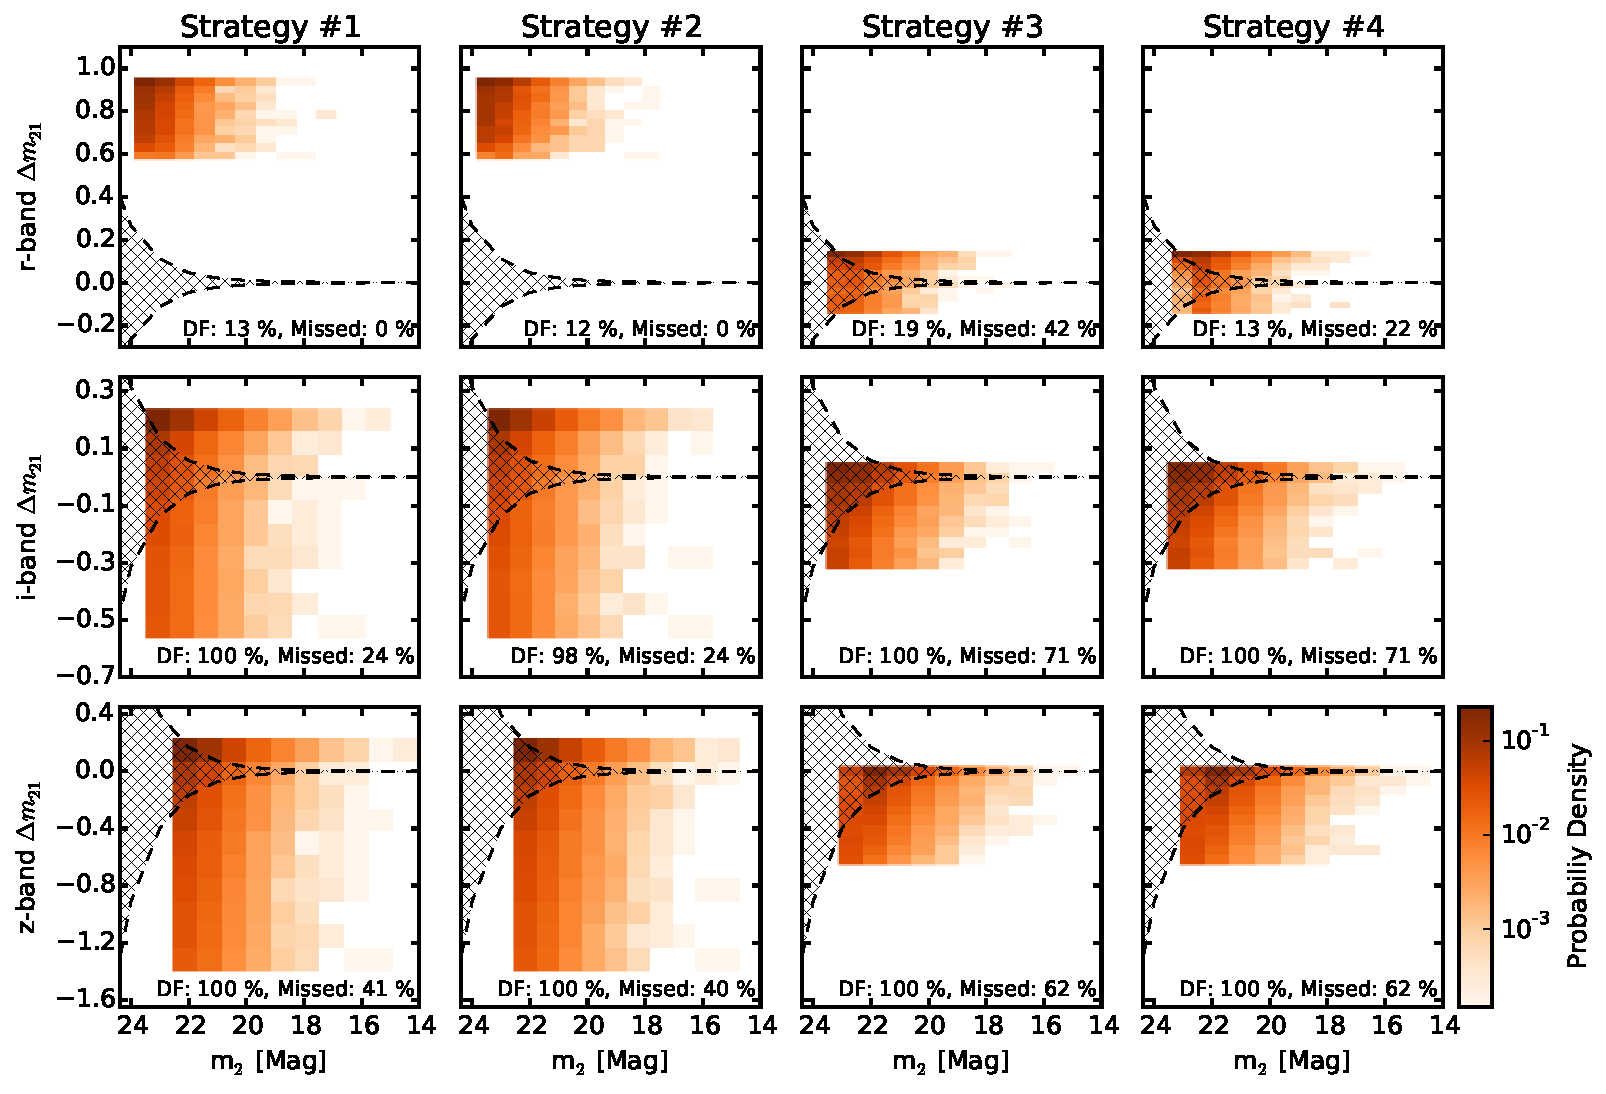
\includegraphics[width=0.9\textwidth]{./figs/chapter2/ch2_f6.pdf}
\caption{Probability density of kilonovae as a function of the change in brightness between the first and second observation $(\Delta m_21)$ versus the brightness in the second observation $(m_2)$ for each of the four observing strategies. The hatched region indicates the $2\sigma$ photometric error for DECam for an exposure time necessary to achieve the required depth. Points within this region will not exhibit a statistically significant change in magnitude for detection. The fraction of sources brighter than the detection limit in all three observations (DF) and the fraction of sources within the hatched region (missed) are indicated at the bottom of each panel. We find that the seemingly beneficial initial rapid cadence of Strategies 3 and 4 on a $\sim$3 hr baseline actually result in a large fraction of brightenings being undetectable.}
\label{fig:ch2_delm2}
\end{figure}
   
In Figure~\ref{fig:ch2_delm2} we plot two-dimensional histograms of $\Delta m_{21}$ versus $m_2$ for each of our four observing strategies and each of the three filters. The resulting histogram is color-coded by the probability of a kilonova falling in that bin, with darker colors indicating a higher probability. We also compute the $2\sigma$ photometric error for an exposure time necessary to reach our chosen target depth in each filter using the DECam exposure calculator\footnote{\url{http://www.ctio.noao.edu/noao/content/Exposure-Time-Calculator-ETC-0}} (hatched region). Sources that exhibit a change in magnitude that is smaller than this photometric error will not produce a statistically significant detection of a change in brightness. Figure~\ref{fig:ch2_delm3} follows a similar construction, showing the two-dimensional histograms for $\Delta m_{31}$ versus $m_3$.

Using these results we determine the fraction of sources that do not exhibit a sufficient change in brightness to be identified as a transient after the second or third observation. We begin by considering the first and second columns of Figures~\ref{fig:ch2_delm2} and~\ref{fig:ch2_delm3} (Strategies 1 and 2). Recall that for these strategies the time between the first and second epoch is $\sim$1 day. In both of these cases, the rapid evolution of the {\em r}-band light curve means that there is always a detectable change in brightness, but the source will always be seen in decline. Furthermore, it is still the case that given the overall faintness of kilonovae in {\em r}-band, only $\sim$13\% of sources will be detected at $r\approx24$ mag.

In {\em i}- and {\em z}-band we find that $(\sim 20-40\%)$ of sources are missed due to an insufficient change in brightness. For Strategies 3 and 4 where the time between the first two observations is only $\sim$3 hr over half of the sources $(60-70\%)$ fail to exhibit a statistically detectable change in brightness. This indicates that the intra-night observations have a time baseline that is too short for detecting a change in brightness even for the fast kilonova timescale.
   
Figure~\ref{fig:ch2_delm3} shows observations that are separated by a longer timescale $(m_3 - m_1)$: For Strategies 1 and 4, the first and third epoch are separated by 2 days, while the same visits are separated by 4 days for Strategy 2, and only 1 day for Strategy 3. For all four strategies we find that {\em r}-band exhibits a sufficient change in brightness, with $\Delta m_{31}$ well outside of the hatched region, but these sources are always observed to decline. As before, only $\sim10-20$\% of the sources are actually detectable at $r\approx24$ mag. In both {\em i}- and {\em z}-band we find that it is possible to detect a change of brightness in a much higher fraction of sources compared to $\Delta m_{21}$. Strategies 1 and 4 both show that $\sim 15-20\%$ of sources will not show a sufficient change in brightness. The highest fraction of missed sources is $\sim 25-40\%$ for Strategy 3. This is expected given the short separation between epochs. Strategy 2, which has the longest separation between epochs, shows only $\sim 10-15 \%$ of sources remaining undetectable. Furthermore, while sources in $r$-band are only observed to decline, in $i$- and $z$-band the rise can also be measured without requiring a $\sim$3 hr baseline. This further highlights the importance of having observations that are sufficiently separated in time to probe the kilonova light curve across a wide range of its evolution.

\begin{figure}[t!]
\centering
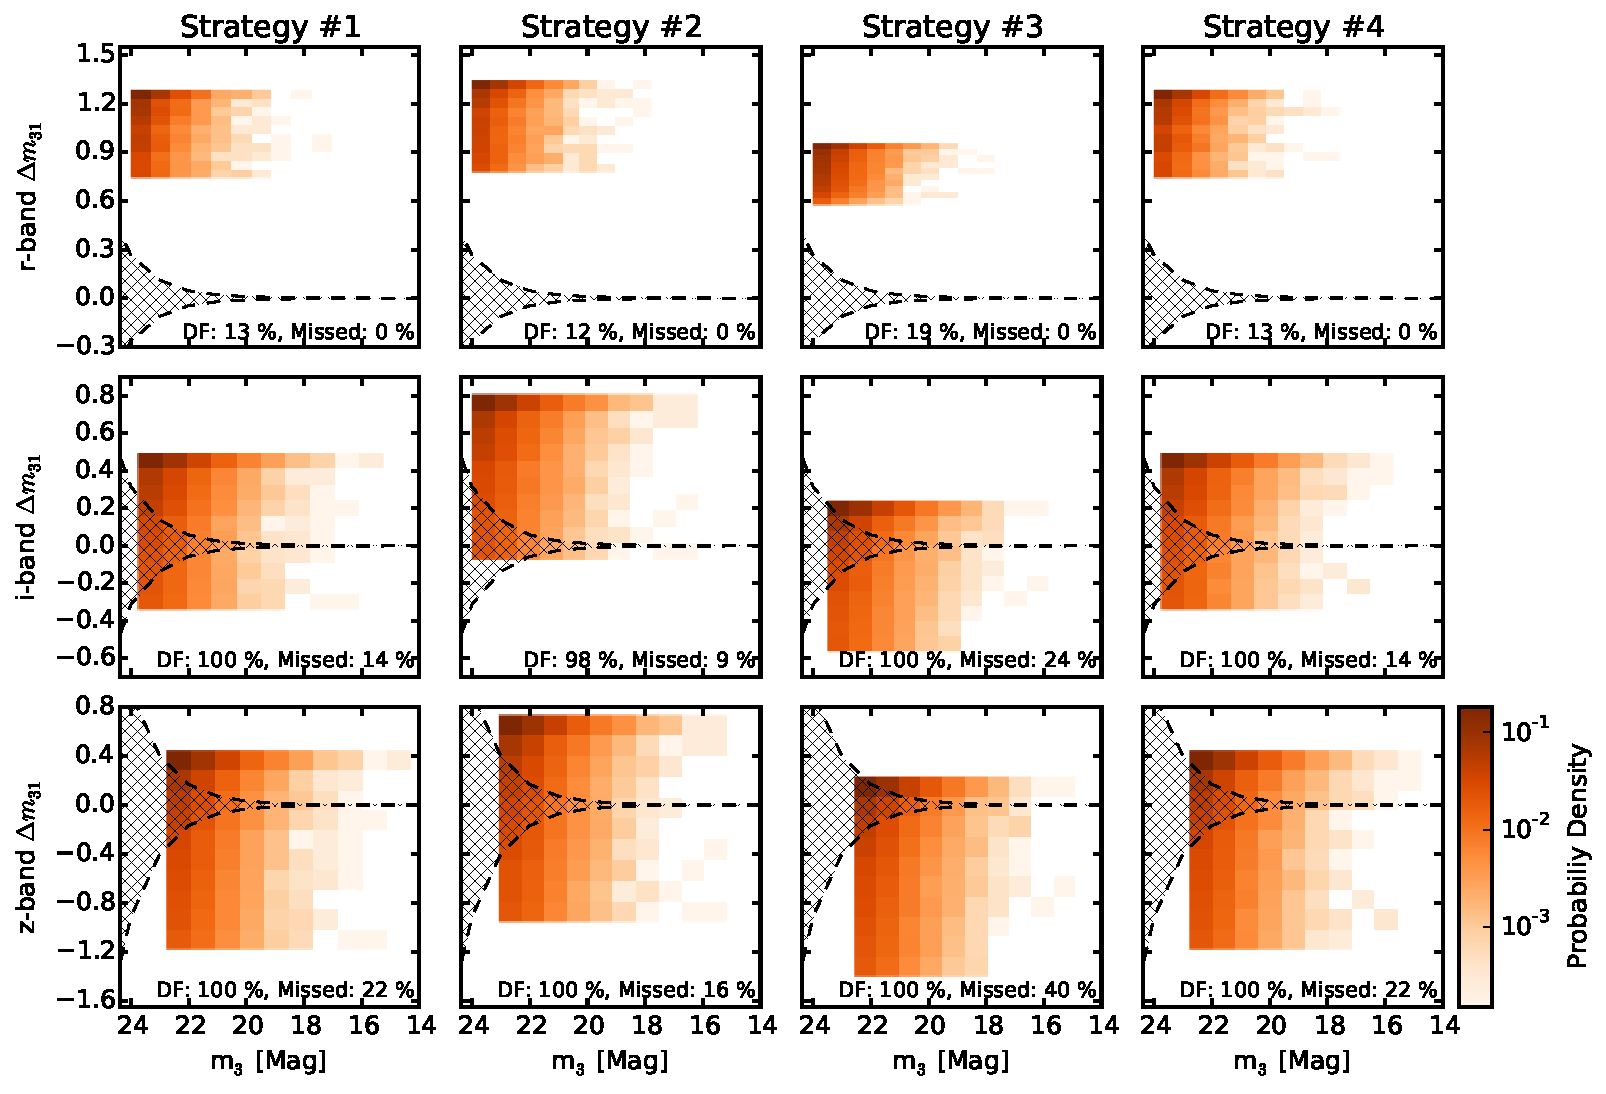
\includegraphics[width=0.9\textwidth]{./figs/chapter2/ch2_f7.pdf}
\caption{Same as Figure~\ref{fig:ch2_delm2}, except we plot the change in brightness between the first and third epoch $(\Delta m_{31})$ versus the brightness in the third epoch $(m_3)$. We find that the increased time between observations allows a much larger fraction of sources to exhibit a detectable change in brightness.}
\label{fig:ch2_delm3}
\end{figure}
   
The rapid decline of $\sim0.6-1.3$ mag in {\em r}-band that is evident in Figures~\ref{fig:ch2_delm2} and~\ref{fig:ch2_delm3} hints at a possible detection strategy. Namely, the GW error region can be observed with a cadence of $\sim$1 d, with rapidly declining sources flagged. However, a depth of $\approx$26 mag is required for a high detection fraction even if we require only 2 detections (to separate kilonovae from stellar flares), so covering the large GW error region can only be achieved with LSST.
   
These detectability simulations indicate that using intra-night observations (Strategies 3 and 4) to detect the rise of the light curve is not an efficient use of time for follow-up observations since kilonovae generally do not exhibit a statistically significant change in brightness on this timescale. As shown in Figure~\ref{fig:ch2_det}, the choice of cadence does not drastically impact the likelihood of detection. Therefore, the most efficient solution, from a detectability standpoint, is Strategy 1. It provides a sufficient cadence to effectively detect kilonovae while maximizing the amount of area that can be covered in a single night. Observations should be carried out in {\em i}- and {\em z}-band as the depths required to detect 95\% of sources $(\approx 24,23$ AB mag, respectively), are obtainable by existing and future facilities.

\subsection{Simulating the Effects of Contamination}
\label{sec:ch2_MCsims_cont}
   
We now use our simulated observations to explore the contaminant population in the framework of the rise time-color-magnitude phase-space outlined in Section~\ref{sec:ch2_phase}. We accomplish this by repeating the simulations for each of the contaminants considered in Section~\ref{sec:ch2_contaminants}. We then utilize the simulated observations to compute analogues to the rise time-color-magnitude phase-space for both kilonovae and the contaminant population. In this manner we can produce a version of the phase-space that takes into account a distribution of contaminants with realistically sampled light curves given the choice of cadence, depth, and start time appropriate to wide-field follow-up observations of a GW trigger.
      
We begin by employing the same four observing strategies as in the previous simulations. We again consider observations at a fixed depth of $\approx$ 24 AB mag in {\em i}-band and $\approx$ 23 AB mag in {\em z}-band, with the observations beginning 3 to 24 hr after the GW trigger. The simulations include 50,000 iterations, each consisting of: (1) A contaminant placed at a random, volume-weighted redshift. We consider contaminants at much larger distances than 200 Mpc to account for the fact that many contaminants are more luminous than kilonovae; the choice of $z_{\text{max}}$ is indicated in Figure~\ref{fig:ch2_mcphasecol}. (2) The contaminant light curve is randomly placed out of phase with respect to the start time of observations. We consider contaminants that occur approximately twice their characteristic timescale prior (5--20 days) and up to 2 days after the start of observations. The latter value is motivated by the results of the previous section in which we showed that kilonovae should be detectable within 1--2 days, and therefore, sources that first appear more than 2 days after the start of the observations can be rejected. Once the phase offset is determined the observation times are computed and the source brightness in {\em i}- and {\em z}-band is computed at each epoch. (3) The observed peak of the {\em z}-band light curve is measured. (4) The {\em i} -- {\em z} color is computed at the epoch where {\em z}-band attains its maximum value. (5) The rise time is defined as the time between the {\em z}-band peak and the first observation in which the source is detected. In cases where the source is only observed in decline, then the decline time is defined as the time between the first observation and the last observation in which the source is detected. 
 
\begin{figure}[t!]
\centering
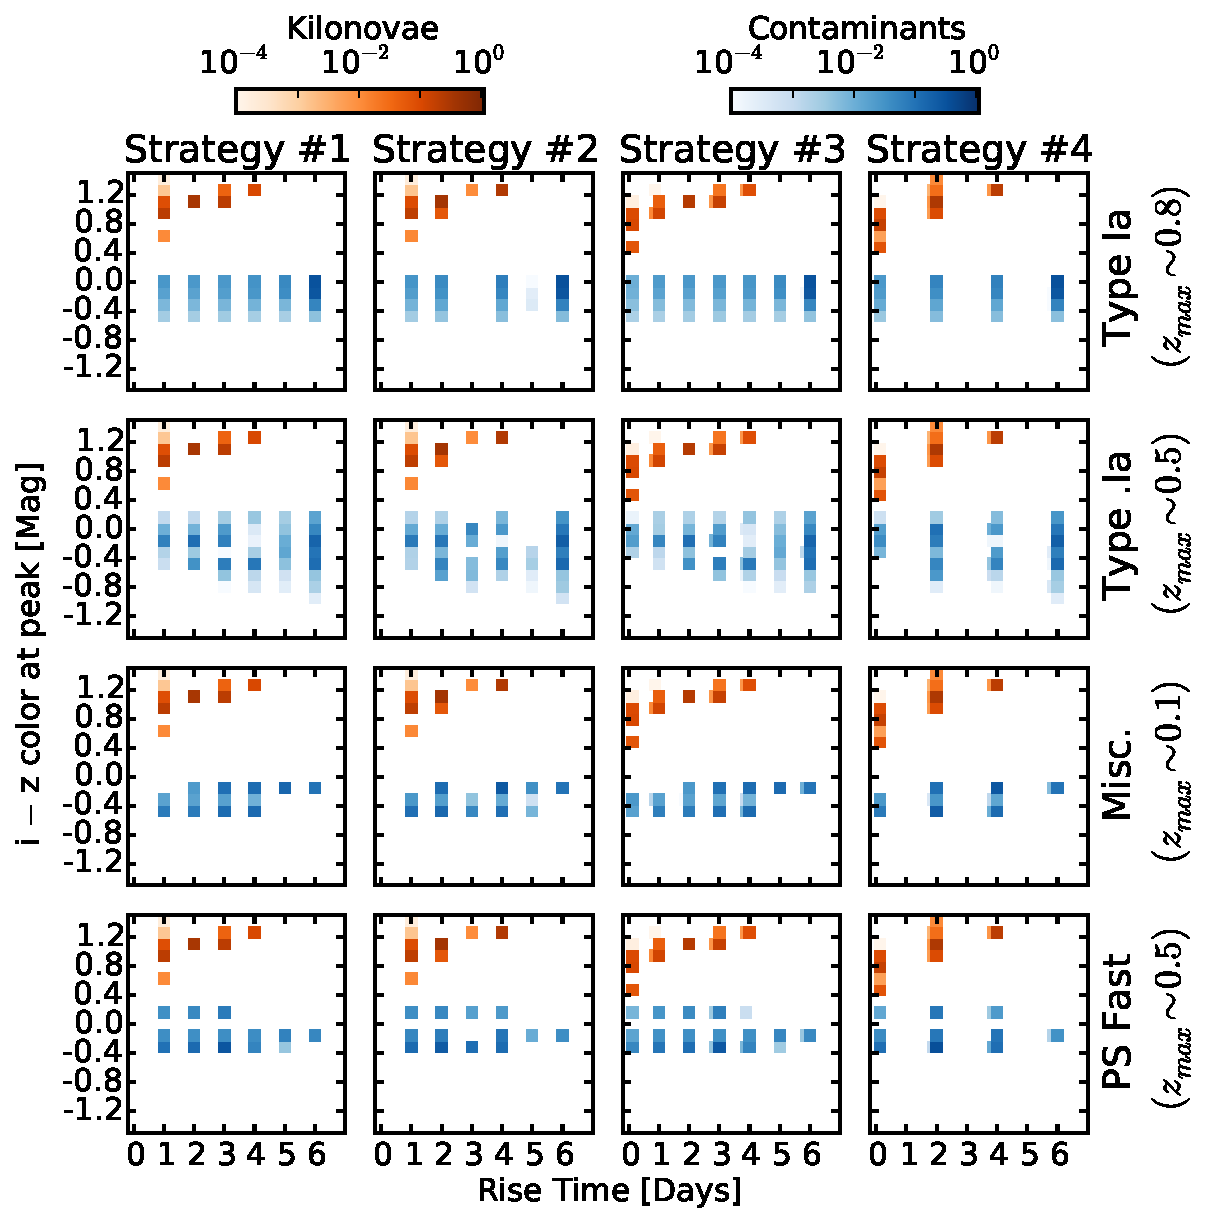
\includegraphics[width=0.9\textwidth]{./figs/chapter2/ch2_f8.pdf}
\caption{Simulated rise time-color phase-space for each of our four observing strategies. In each panel, we consider the full grid of kilonova models to a distance of 200 Mpc (orange). Each row highlights a different subset of the contaminant population over the comoving volume to $z_{\text{max}}$ (blue). The offset bins for Strategies 3 and 4 are due to the availability of intra-night observations on the first night. We find that the kilonovae are much redder than any potential contaminant, but the separation is less well-defined when compared to the light curves used in Section~\ref{sec:ch2_phase}.}
\label{fig:ch2_mcphasecol}
\end{figure}
   
In Figure~\ref{fig:ch2_mcphasecol} we plot the rise time-color slice of the three-dimensional phase-space for each observing strategy. In addition to the nine kilonovae models, we consider four groups of sources with each given an equal contribution. The first group of contaminants is Type Ia SNe (Figure~\ref{fig:ch2_mcphasecol}, first row). The second group is comprised of the four type .Ia SNe models (Figure~\ref{fig:ch2_mcphasecol}, second row). We form the third group from all of the low luminosity, fast transients (i.e., AIC, WD-NS/BH mergers, and ELDD; Figure~\ref{fig:ch2_mcphasecol}, third row). Lastly, the fourth group of contaminants contains the three Pan-STARRS fast transients (Figure~\ref{fig:ch2_mcphasecol}, fourth row).
   
To analyze the results, we first bin sources by their rise times, which fall in discrete values due to the cadence of the observations. For each rise time bin, we then bin the source populations by $i-z$ color in equally spaced bins from --1.5 to +1.5 mag. For each bin, we compute the fraction of detected sources in that bin relative to the total number of detected sources.

As we showed in Section~\ref{sec:ch2_phase}, kilonovae stand out from the contaminant population primarily on the basis of their redder colors, even when luminous contaminants are considered to higher redshifts (e.g., Type Ia SNe, Pan-STARRS fast transients). For all choices of observing strategy there is essentially no overlap in $i-z$ color between the kilonova population and any of the contaminant populations. We note that across all four observing strategies $\sim$12\% of Type Ia SNe, $\sim7\%$ of type .Ia, and $\sim8\%$ of Pan-STARRS fast transients exhibit $i-z\gtrsim 0$, while none have $i-z\gtrsim0.4$ mag. However, all kilonovae exhibit $i-z\gtrsim0.4$ mag. These numbers are relative to the total number of events observed during the rise and do not include sources that are observed only in decline (see below). Consequently, $i-z$ color remains a strong discriminant for separating kilonovae from the contaminant population. 
   
So far we have neglected the potential effect of extinction in reddening the $i-z$ colors of the contaminant sources. If the extinction is sufficiently large an intrinsically blue contaminant may be reddened into the regime of kilonova $i-z$ colors. However, this extinction will also cause the source to appear dimmer and may therefore push it below the detection limit. To quantify the effects of extinction we use the Milky Way extinction curve with $R_V = 3.1$. Figure~\ref{fig:ch2_mcphasecol} indicates that a reddening of $E(i-z) \approx 1$ mag is required to shift the contaminant population into the region of phase-space occupied by kilonovae. This will result in an extinction of $A_V \approx 6.3$ mag, $A_i \approx 3.9$ mag and $A_z \approx 2.9$ mag.  However, in our simulation nearly all ($\gtrsim 97\%$) of the contaminants which pass the detection cuts have $m_z \gtrsim 20$ mag meaning that an extinction of 2.9 mag will dim these sources below our {\em z}-band detection limit of $\approx$ 23 mag. Thus, reddening due to dust extinction does not seem to be a concern.
   
We also consider the possibility of separating kilonovae by their rise time. In Figure~\ref{fig:ch2_phase}, the entire set of kilonovae models showed generally shorter timescales relative to the contaminant population with rise times of $\lesssim4$ days. However, when the contaminants are placed out of phase with the GW trigger, and the observing cadence is taken into account, we find contaminants that present an apparent shorter rise time. This effect is the most prominent in the Pan-STARRS fast transients and miscellaneous fast transients for which $\sim55-60\%$ and $\sim65-75\%$ of detected sources show a rise time of $\lesssim$ 4 days, respectively. We also find that $\sim 35-45\%$ of detected type .Ia show a rise time that is $\lesssim$ 4 days. Lastly, for Type Ia SNe, $\sim20-25\%$ of detected sources will present a rise time of $\lesssim$ 4 days. Thus, rise time alone is not a strong discriminant for separating kilonovae from the contaminant population.
   
\begin{figure}[t!]
\centering
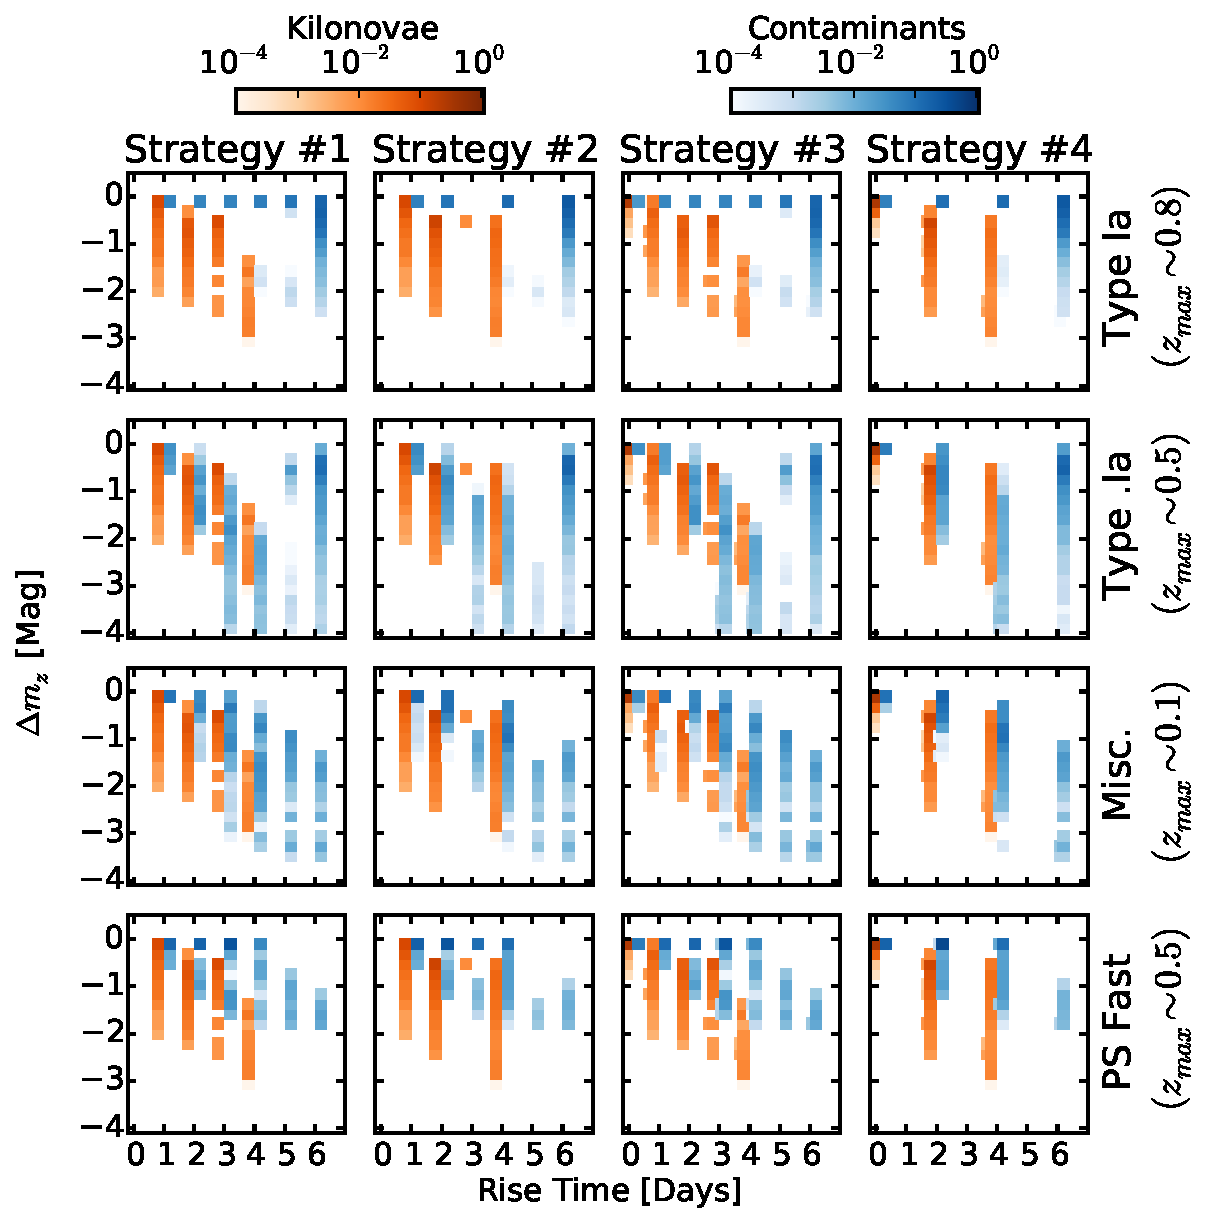
\includegraphics[width=0.9\textwidth]{./figs/chapter2/ch2_f9.pdf}
\caption{Same as Figure~\ref{fig:ch2_mcphasecol}, but showing the simulated rise time-$\Delta m_z$ slice of the phase-space. In this slice, there is much more confusion between the kilonovae and contaminant populations. With the exception of Type Ia SNe, there is significant overlap between kilonovae and the contaminant populations. This is the result of considering rapidly evolving sources for our contaminants, and it highlights the importance of color information in the selection of kilonovae candidates.}
\label{fig:ch2_mcphasedm}
\end{figure}
   
In Section~\ref{sec:ch2_phase}, we considered the peak {\em z}-band magnitude as the third data point in our phase-space. However, in a magnitude limited search, the population of contaminants will be dominated by events at the furthest distance to which they can be detected. Here we instead track the evolution of the source brightness by computing the difference in {\em z}-band magnitude between the source at the observed peak ($m_{z,{\rm peak}}$) and the first observation in which it is detected ($m_{z,0}$), denoted as $\Delta m_z \equiv m_{z,{\rm peak}} - m_{z,0}$. We show the rise time-$\Delta m_z$ slice of the three-dimensional phase-space in Figure~\ref{fig:ch2_mcphasedm}. The basic layout of the figure is identical to that of Figure~\ref{fig:ch2_mcphasecol}, but sources are offset by $\pm$5 hours to improve visibility.
   
We find that kilonovae exhibit $\Delta m_z \approx -3.5\text{ to }0$ mag, where larger changes in brightness are associated with longer rise times. Type Ia SNe only exhibit values of $\Delta m_z$ comparable to those of kilonova when the observed rise time is $\sim6$ d (the duration of our search), well beyond the range of observed rise times for kilonovae. When the rise time is $\lesssim6$ d, the average change in brightness is negligible ($\Delta m_z \approx 0.05$ mag). This is because shorter rise times only occur near peak when the light curve evolution is slow. This slow evolution will make Type Ia SNe easy to reject relative to the much more rapidly evolving kilonovae. We note a small fraction of events with $\Delta m_z \approx -2$ mag and rise times of $4-5$ days. These account for $\lesssim0.2\%$ of detected Type Ia SNe and are the result of an event occurring in a range of redshifts where the set of spectral features that produce the second peak of Type Ia SNe appear in {\em z}-band. Thus, Type Ia SNe can be rejected based on $\Delta m_z$, rise time, and $i-z$ color. For the other contaminant populations the separation is not as clean. This is not unexpected since rapid evolution was a strong consideration when constructing our list of potential contaminants. This highlights the critical importance of selecting kilonovae on the basis of their $i-z$ color along with their rapid rise times. 
   
\begin{figure}[t!]
\centering
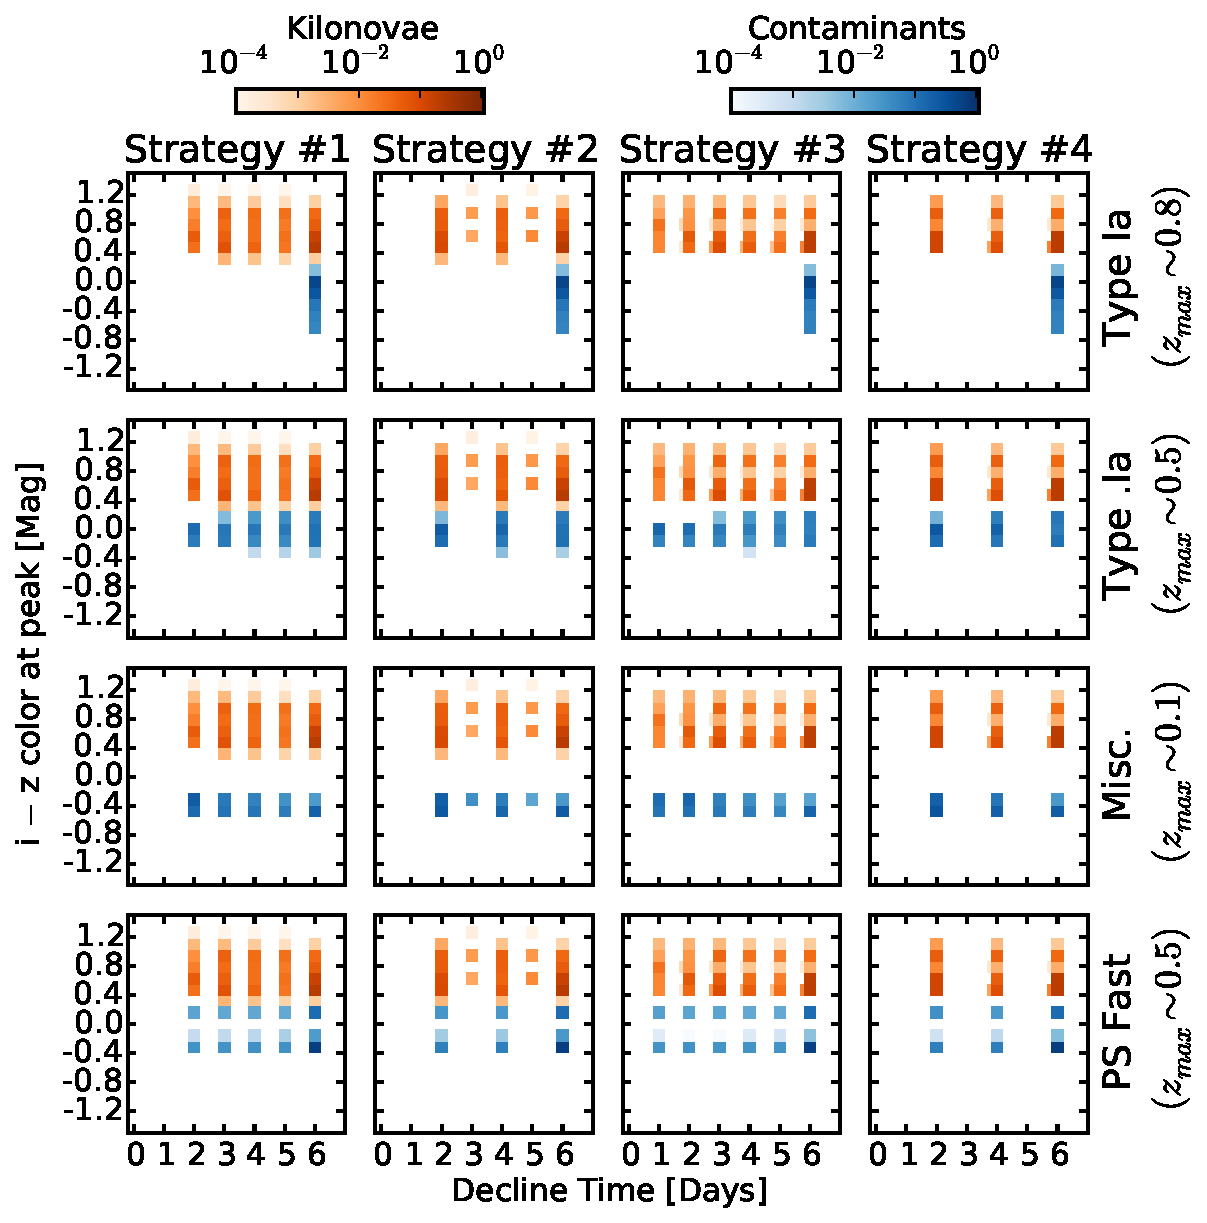
\includegraphics[width=0.9\textwidth]{./figs/chapter2/ch2_f10.pdf}
\caption{The decline time-color slice of the decline time-color-magnitude phase-space. The plot is constructed using the same methodology as in Figures~\ref{fig:ch2_mcphasecol} and~\ref{fig:ch2_mcphasedm}. We note that, as before, kilonovae show redder $i-z$ colors than the contaminant population. However, there is no strong separation in decline time.}
\label{fig:ch2_deccol}
\end{figure}
   
We demonstrated in Figure~\ref{fig:ch2_rise} that it is challenging to detect a kilonova during the rise to peak. Therefore, in our simulations we also consider the behavior of sources that are observed in decline. We construct an identical phase-space by replacing the rise time with the decline time, as defined above. Figure~\ref{fig:ch2_deccol} shows the decline time-color slice of this phase-space. The layout is identical to Figure~\ref{fig:ch2_mcphasecol}. As before, the kilonova population presents $i-z$ colors that are consistently redder than those of the contaminant population with all detected events exhibiting $i-z \gtrsim 0.3$ mag. Furthermore, the fraction of contaminants seen in decline that exhibit $i-z\gtrsim0$ is essentially unchanged compared to those observed on the rise. Additionally, all of the contaminants considered still exhibit $i-z \lesssim 0.3$ mag, so therefore color can still be utilized as a strong discriminant. 
   
The efficacy of a cut on decline time is diminished compared to a cut on rise time. Both kilonovae and the contaminant population cover the entire distribution of possible decline times from $\sim2-6$ days. A notable exception is Type Ia SNe, which all exhibit a decline time of $\sim6$ days (the duration of the search), because if the source is already in decline at the start of the observations, it will remain detectable for the entire duration of the search. Only $\sim20-25\%$ of kilonovae exhibit a decline time of $\lesssim6$ days, making this an ineffectual cut. On the other hand, the slow evolution is beneficial for separating the Type Ia SNe population from a kilonova if template images at $\gtrsim 10$ days are utilized. In this scenario, the kilonova will have faded away while Type Ia SNe will remain visible allowing them to be easily rejected. 

\begin{figure}[t!]
\centering
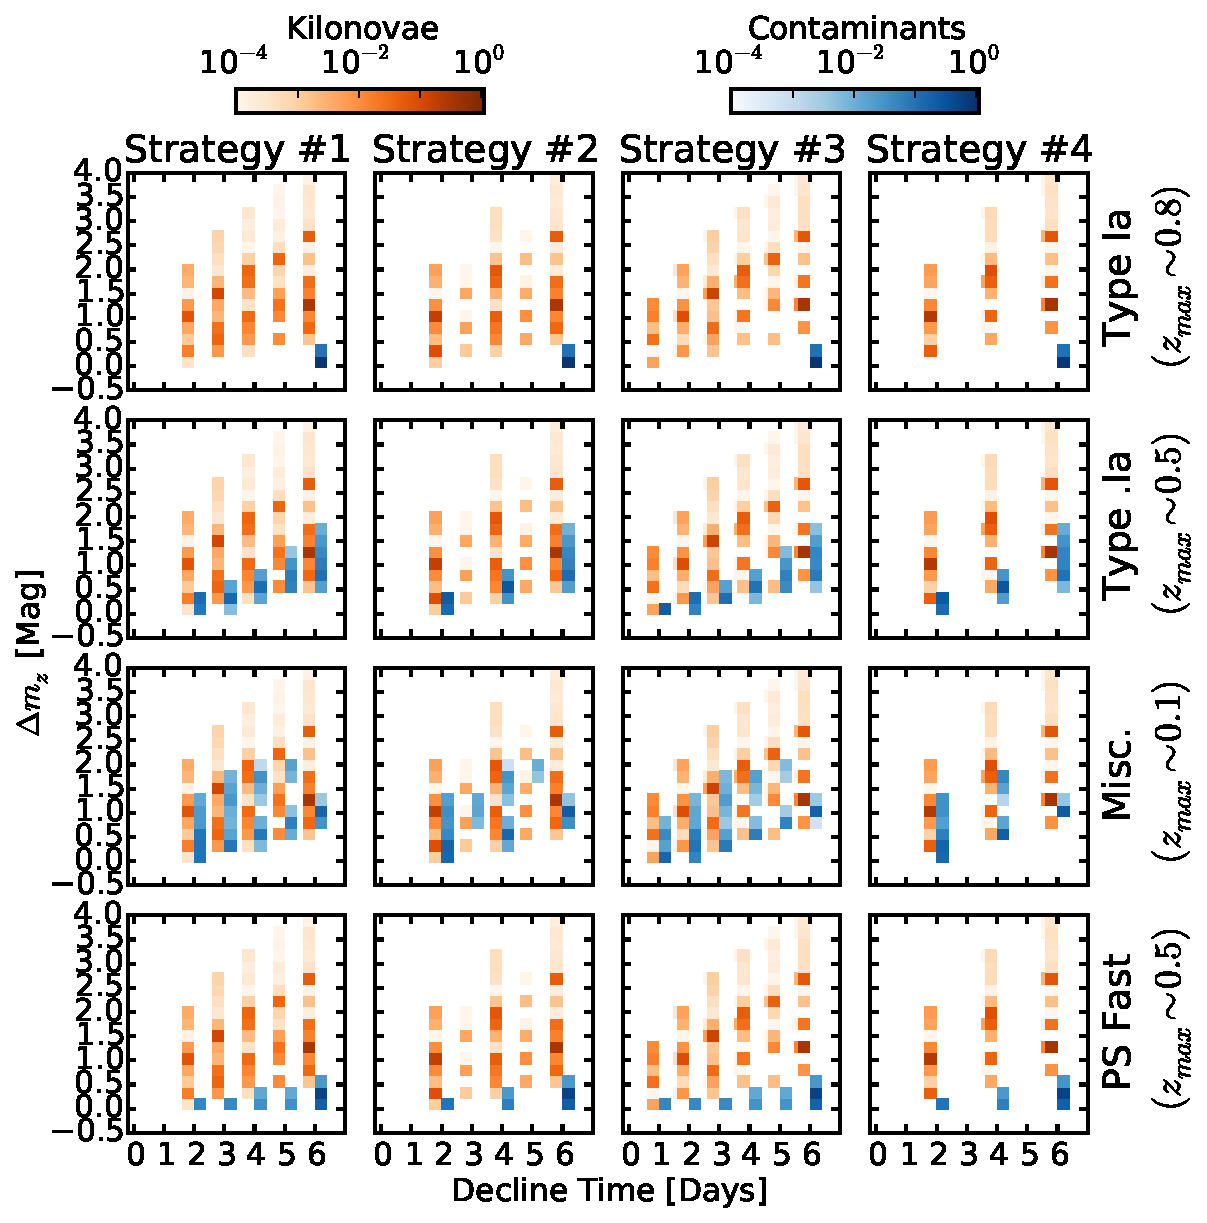
\includegraphics[width=0.9\textwidth]{./figs/chapter2/ch2_f11.pdf}
\caption{The decline time-$\Delta m_z$ slice of the decline time-color-magnitude phase-space. The slow decline of Type Ia SNe and the Pan-STARRS fast transients separate them from the rapidly evolving kilonovae. However, the type .Ia and the miscellaneous fast transients show changes in brightness comparable to those of kilonovae.}
\label{fig:ch2_decdm}
\end{figure}
   
Figure~\ref{fig:ch2_decdm} shows the decline time-$\Delta m_z$ slice of the phase-space. In this context we define $\Delta m_z \equiv m_{z,{\rm last}} - m_{z,{\rm 0}}$, where $m_{z,{\rm last}}$ is the {\em z}-band magnitude from the last observation in which the source is detected. Kilonovae exhibit a change in brightness of $\Delta m_z \approx 0 - 4$ mag, with a weak trend for larger changes in brightness being associated with longer observed decline times. The Type Ia SNe and Pan-STARRS fast transients exhibit an average change in brightness of only $\Delta m_z \approx 0.1$ mag and $\Delta m_z \approx 0.2$ mag, respectively, making the potential for contamination low. However, as with the rise time-$\Delta m_z$ space, the type .Ia and miscellaneous fast transients exhibit changes in brightness that are comparable to those of kilonovae. This makes cuts on $\Delta m_z$ less practical for these sources.  

The key point emerging from our simulations is that $i-z$ color is a strong discriminant for selecting kilonovae, regardless of observing strategy, and whether a kilonova is observed on the rise or decline. In fact, if we consider sources observed during the rise to peak, and we require that $i-z\gtrsim0$ mag we may eliminate $\sim84-87\%$ of detected Type Ia SNe and Pan-STARRS fast transients, $\sim90-94\%$ of detected type .Ia, and $\sim100\%$ of detected miscellaneous fast transients without removing any kilonovae from the selection. If we additionally require that the rise time is $\lesssim4$ days, then we eliminate $\sim94\%$ of detected Type Ia SNe and $\sim98\%$ of detected type .Ia. If we also require that $|\Delta m_z| \gtrsim 0.1$ mag, we eliminate $\sim99\%$ of Type Ia SNe.

Considering sources observed in decline the cuts on $i-z$ color and $\Delta m_z$ remain effective but a cut on decline time does not provide any additional information. Quantitatively, if we apply cuts of $i-z \gtrsim 0$ mag and $|\Delta m_z| \gtrsim 0.1$ mag we eliminate $\sim80\%$ of Type Ia SNe, $\sim60\%$ of type .Ia, $\sim81\%$ of Pan-STARRS fast transients, and $\sim 100\%$ of the miscellaneous fast transients. If we also require that the decline time is $\lesssim 5$ days we eliminate $\sim 100\%$ of the Type Ia SNe and $\sim94\%$ of the Pan-STARRS fast transients, but lose $\sim46\%$ of the kilonova population. However, if additional observations are taken at $\gtrsim10$ days then these kilonovae can be recovered. But, given that cuts made on sources observed to rise are more effective, then in order to maximize the chances of a kilonova detection and identification during a GW follow-up campaign it is essential to obtain both {\em i}- and {\em z}-band data as close to the GW trigger as possible. 

\section{Counterpart Identification In The Absence of a Template} 
\label{sec:ch2_diff}
We now investigate the situation where there are no pre-existing template images of the GW error region and we would like to rapidly identify a kilonovae without having to wait for a late-time template. This scenario introduces several challenges. Foremost is the presence of source flux in the image that will be used as a template, which will have an effect on the observables (e.g., brightness, color). Specifically, we can no longer measure the true flux of the source but rather only the difference in flux between the science and template images. In this case, a measurement of the true magnitude of the source is impossible. Without the accurate measurement of source brightness it is also difficult to measure the true color and we therefore lose one of the primary methods of distinguishing kilonovae from the contaminant population. As discussed in detail below, these difficulties can be alleviated by making simple assumptions about the source behavior. 
   
Another obvious challenge is a delay in the timescale of the first science image since the first observation must be used as the template image. This is leads to problems in characterizing  the early behavior of the light curve, as well as in utilizing the rise time as a method of distinguishing kilonvoae from the contaminant population. Using the first observation as a template also reduces the number of available epochs making it more difficult to meet the detection criteria outlined in the previous section. However, these challenges are less severe as they can resolved using a late-time template once potential counterparts are identified.   
   
To address the scenario of using the first image as a template, and to gauge the associated complications, we simulate observations using the same methodology outlined in Section~\ref{sec:ch2_MCsims_det}, but taking into account the fact that the first observation is the template. The general procedure is identical to the previous simulations with the following modifications: We now simulate the effects of difference imaging by subtracting the flux in the first observation (the template) from the later observations (the science images) to produce a set of difference fluxes. We account for the noise appropriately by using our search depth as a $5\sigma$ flux limit. We assume that this noise is the dominant source of error and that it is the same for all images. The noise in the difference image is then larger by a factor of $\sqrt{2}$ than that of the individual images. Any source that shows a change in flux with a signal-to-noise ratio (SNR) greater than 5 in the difference image in at least two subtractions is flagged as a detection. If a source exhibits at least one epoch with a positive change in flux, the event is flagged as ``rising."

\begin{figure}[t!]
\centering
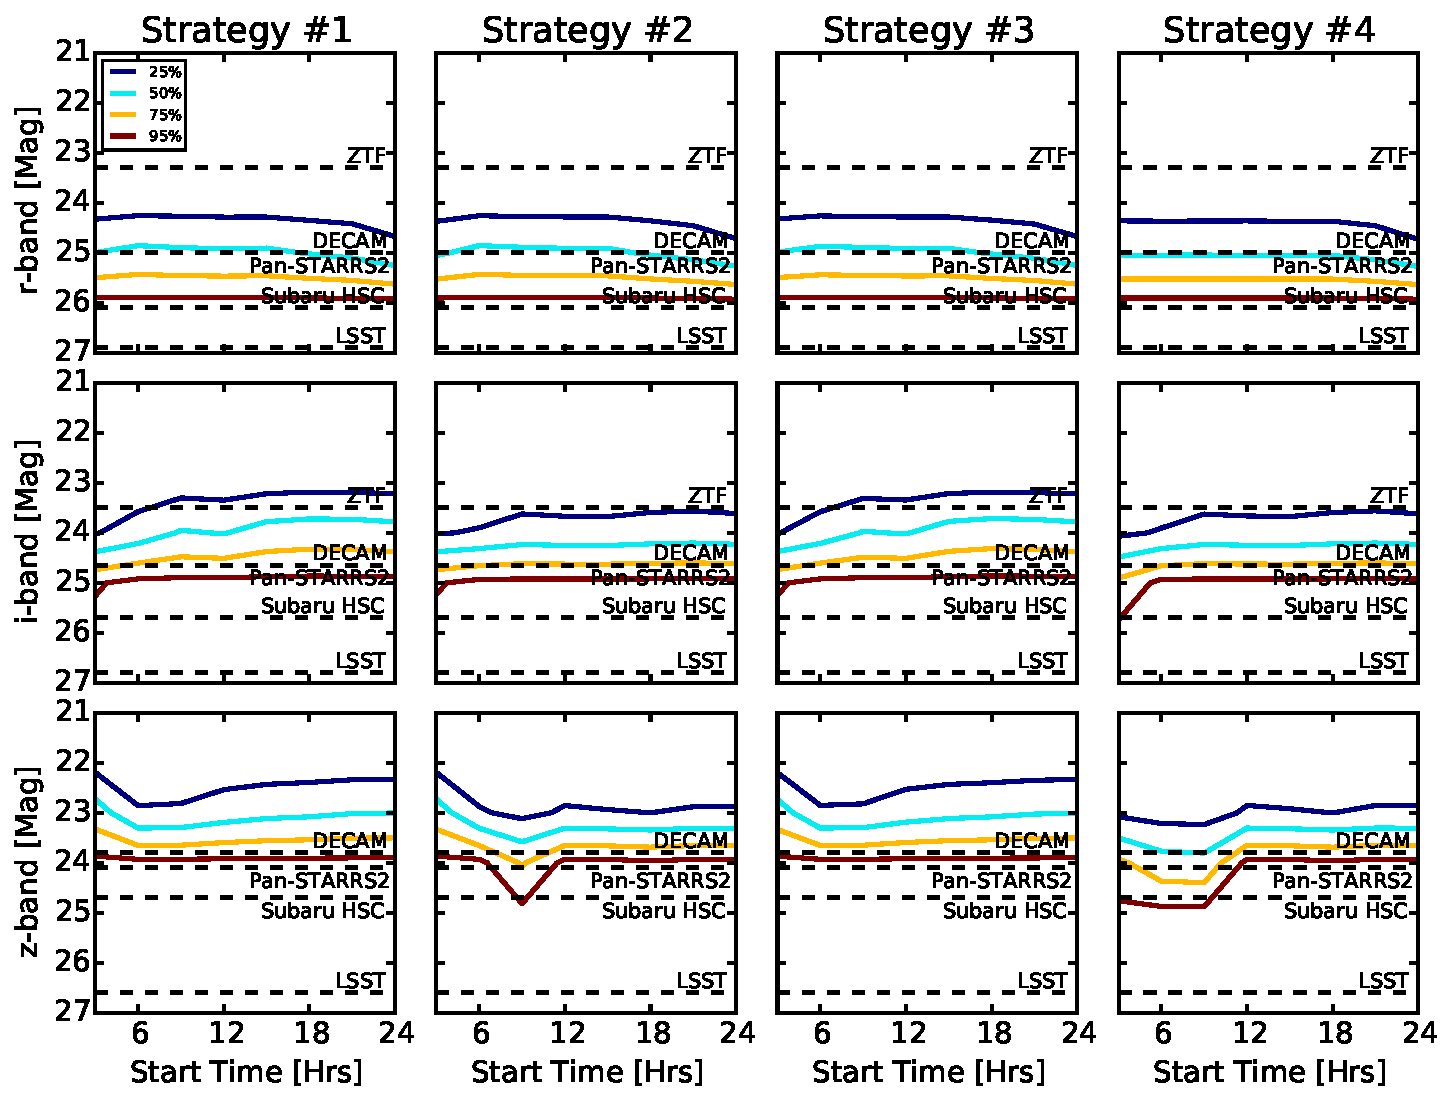
\includegraphics[width=0.9\textwidth]{./figs/chapter2/ch2_f12.pdf}
\caption{Contours showing the fraction of kilonovae detected as a function of start time and depth for our four observing strategies and three filters when a pre-existing template is not available. We first note that $i$- and $z$-band observations in this scenario must be $\sim1$ mag deeper to achieve detection rates comparable to when a pre-existing template is available. We also note an effect in {\em z}-band where the 95\% contour drops by $\sim1$ mag for observations starting between 6 and 12 hours after trigger using Strategy 2 and for observations starting less than 12 hours after the trigger using Strategy 4. This is the result of the observations straddling the peak of the light curve where the difference in flux between epochs is too small to detect.}
\label{fig:ch2_detdiff}
\end{figure}

In Figure~\ref{fig:ch2_detdiff}, we plot contours of the fraction of sources that pass our detection criterion as a function of start time and search depth. The layout of this plot is identical to that of Figure~\ref{fig:ch2_det}. We first note that the {\em r}-band contours for Strategies 1 and 2 are essentially identical to those in Figure~\ref{fig:ch2_det}. This is because the $r$-band light curve evolves fast enough between observations that the effects of using the first observation as a template does not hamper detections. However, for Strategies 3 and 4, we no longer find the early-time ($\lesssim6$ hours) boost in detection limit. This is due to the fact that the light curve does not change sufficiently during the three hours, and the source is therefore not detected in the first difference image. There is therefore no benefit from the additional observation on the first night. On the other hand, in {\em i}-band we find that on average the depth required to reach a certain detection rate is $\sim 1$ mag deeper than in the case of a pre-existing or late-time template (Figure~\ref{fig:ch2_det}). Specifically, for Strategy 1 the 50\% contour starts at $\approx24.4$ mag for $t_{{\rm start}} \sim 3$ hours and rises to $\approx 23.7$ mag by $t_{{\rm start}} \sim24$ hours. In Strategy 2, the 50\% contour is flat at $\approx24.3$ mag. The 95\% contour is flat at $\approx25$ mag in both cases. Strategy 3 is identical to Strategy 1, again highlighting the fact that the rapid cadence on the first night does not boost the detection rate. Lastly, we find that the rapid early-time cadence combined with the slow late-time cadence of Strategy 4 actually produces a drop in efficiency for observations beginning at $\sim$ 3 hours where the 95\% contour dips to $\approx 25.7$ mag.

The most pronounced change relative to the case of a pre-existing template (Figure~\ref{fig:ch2_det}) can be seen in the {\em z}-band contours. In Strategy 1, the 50\% (95\%) contour is approximately $\approx 23\,(23.9)$ mag, which is again $\sim 1$ mag deeper than for the case of a pre-existing template. Strategy 2 shows a change of behavior in the 95\% contour between 6 and 12 hours, where the required depth dips to $\approx 24.8$ mag. This is because observations starting during this time frame will be roughly symmetrical about the peak of the light curve. Therefore, the change in flux is small and the source will not be detected in the difference image. The slow cadence of Strategy 2 then makes it difficult to obtain enough observations to reach our threshold for a detection. This effect is also seen in Strategy 4 where the 95\% contour dips to $\approx 24.8$ mag for any starting time less than 12 hours. These contours are summarized in Table~\ref{tab:ch2_det}.

\begin{figure}[t!]
\centering
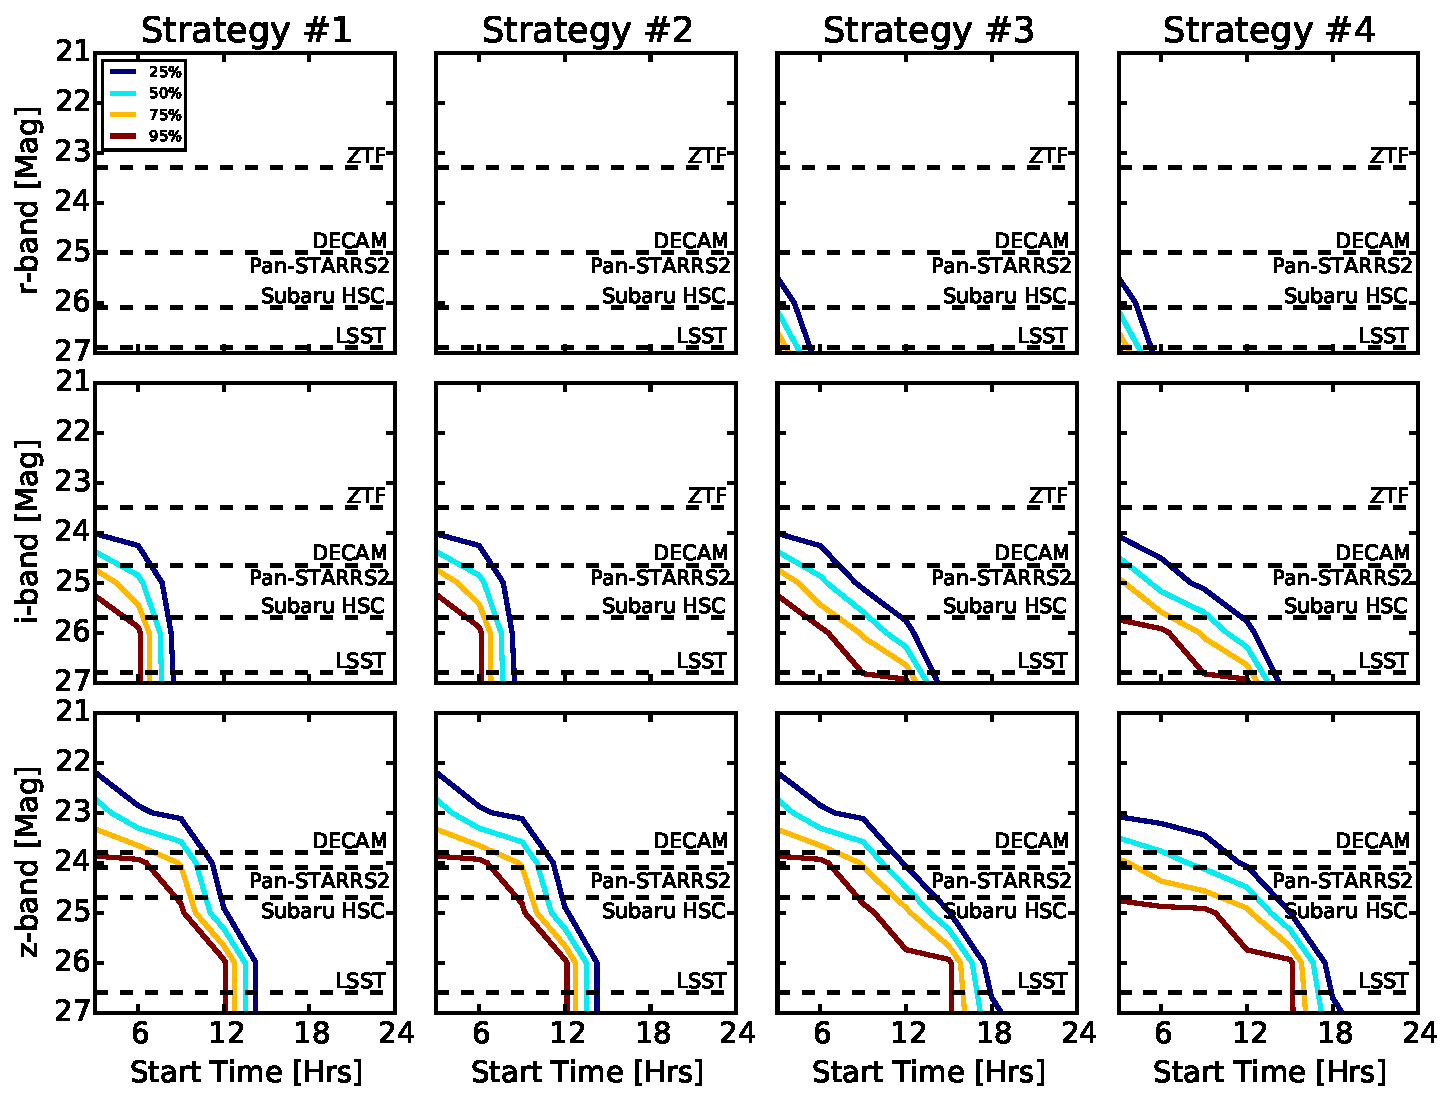
\includegraphics[width=0.9\textwidth]{./figs/chapter2/ch2_f13.pdf}
\caption{Same as Figure~\ref{fig:ch2_detdiff}, but showing the fraction of sources for which brightening is detected. We note that when compared to the contours shown in Figure~\ref{fig:ch2_rise} for the case of a pre-existing template, observations must go deeper in this scenario and the detection efficiency quickly tapers off as a function of starting time. This highlights the importance of commencing follow-up observations as soon as possible when a pre-existing template is not available.}
\label{fig:ch2_risediff}
\end{figure}
   
In Figure~\ref{fig:ch2_risediff}, we show contours for the fraction of sources with a detected brightening between the template and at least one of the science images. These sources must also pass the detection criterion described above. The layout is identical to that of Figure~\ref{fig:ch2_rise}. The behavior of the contours is different compared to the case of a pre-existing template for all bandpasses and strategies. In Figure~\ref{fig:ch2_rise}, the contours were flat and then exhibited a sharp drop off when the first observation began post peak. Here, the contours show a steady decline as a function of start time. This is because as the start time of the first observation (i.e., the template) approaches the peak, the observed change in flux will decrease. Therefore, it becomes progressively more difficult to detect a brightening and the required depth increases.

Specifically, for {\em r}-band, no brightening is detected when utilizing Strategies 1 and 2. The same is effectively true for Strategies 3 and 4, unless the observations reach a depth of $\approx 26.2$ mag and begin $\lesssim$ 3 hr after the GW trigger. Thus, even with deep Subaru HSC or LSST observations, brightening could only be detected in $\sim25-50$\% of sources for observations starting within 3 hours of the GW trigger. In {\em i}-band, for Strategies 1 and 2, the 50\% (95\%) contour begins at $\approx 24.4$ (25.3) mag and no rise is detected if $t_{{\rm start}} \gtrsim 7$ (6) hours. For Strategies 3 and 4, the 50\% (95\%) contours start at $\approx 24.5\,(25.3)$ mag and fall below the LSST limiting magnitude by $\sim 9\,(6)$ hours. Thus, the detection of a rise in $i$-band is not feasible with existing telescopes without a pre-existing template. Lastly, for {\em z}-band, the 50\% (95\%) contours in Strategies 1 and 2 begin at $\approx 22.7\,(23.9)$ mag and fall below the LSST limiting magnitude by $\sim 15\,(12)$ hours. For Strategy 3, the required depths are unchanged compared to Strategies 1 and 2, but the 50\%(95\%) contours extend out to $\sim 17\,(15)$ hours. For Strategy 4, the required depth to achieve a 50\% (95\%) detection rate is $\sim 1$ magnitude deeper compared to Strategy 3, but the required start times are identical. As above, this is possible with Subaru HSC and LSST, but other instruments (e.g., DECam, Pan-STARRS2) will only be able to achieve a 95\% detection rate for $z$-band observations starting within $\sim6$ hours of the GW trigger. This highlights the increased difficulty in characterizing the early-time behavior of the light curve because we lose information from the first epoch when it is used as the template image. We note that this information can be recovered after the fact using a late-time template but here we are concerned with rapid identification.

\subsection{Contaminant Rejection In The Absence of a Template}
\label{sec:ch2_rejection}
We now investigate how the absence of a pre-existing template affects our ability to reject contaminants. We carry out our simulations in the following way. The flux in the first observation (the template) is subtracted off from the later observations. Noise calculations are handled identically to those outlined above for the detectability simulation, and we impose the same detection criterion for events. The rise/decline time phase-space coordinates are computed using the same definition as in Section~\ref{sec:ch2_MCsims_cont}. The challenge then is computing an analogue for the values of the $i-z$ color and $\Delta m_z$ when the source flux is not known absolutely (due to the presence of source flux in the template image). 

When there is source flux in the template image we are only able to measure a difference in flux between the template and science image. We denote this as $\Delta f_{\phi} \equiv f_{s,\phi} - f_{t,\phi}$ where $f_{s,\phi}$ is the flux observed in the science image and $f_{t,\phi}$ is the flux observed in the template image, both in some bandpass $\phi$. We can then define an AB magnitude using the standard formula $m^{\star}_{\phi} = -2.5\log{|\Delta f_{\phi}|}-48.6$, where the star denotes magnitudes computed from a difference in flux. The $\phi_1 - \phi_2$ color for bandpasses $\phi_1$ and $\phi_2$ is then $m^{\star}_{\phi_1} - m^{\star}_{\phi_2}$. In the case that $|\Delta f_{\phi}|$ is large, and consequently the detection is of high statistical significance,  we approach the limit where the source flux in the template is negligible and a reasonable approximation for the true magnitude and color of the source can be obtained. However, for less significant detections, the measured color will not be an accurate measurement of its true value.

Lastly, we construct a straight-forward analogue to the rise/decline time-$\Delta m$ slice of our phase-space. In the case of a rising source, we compute $m^{\star}_z$ using the largest positive difference in flux between the template image and the science images. If the source is observed only in decline then the largest negative difference in flux is used. This will allow us to understand how rapidly a source evolves relative to others in this study (e.g., kilonovae versus contaminants).

\begin{figure}[t!]
\centering
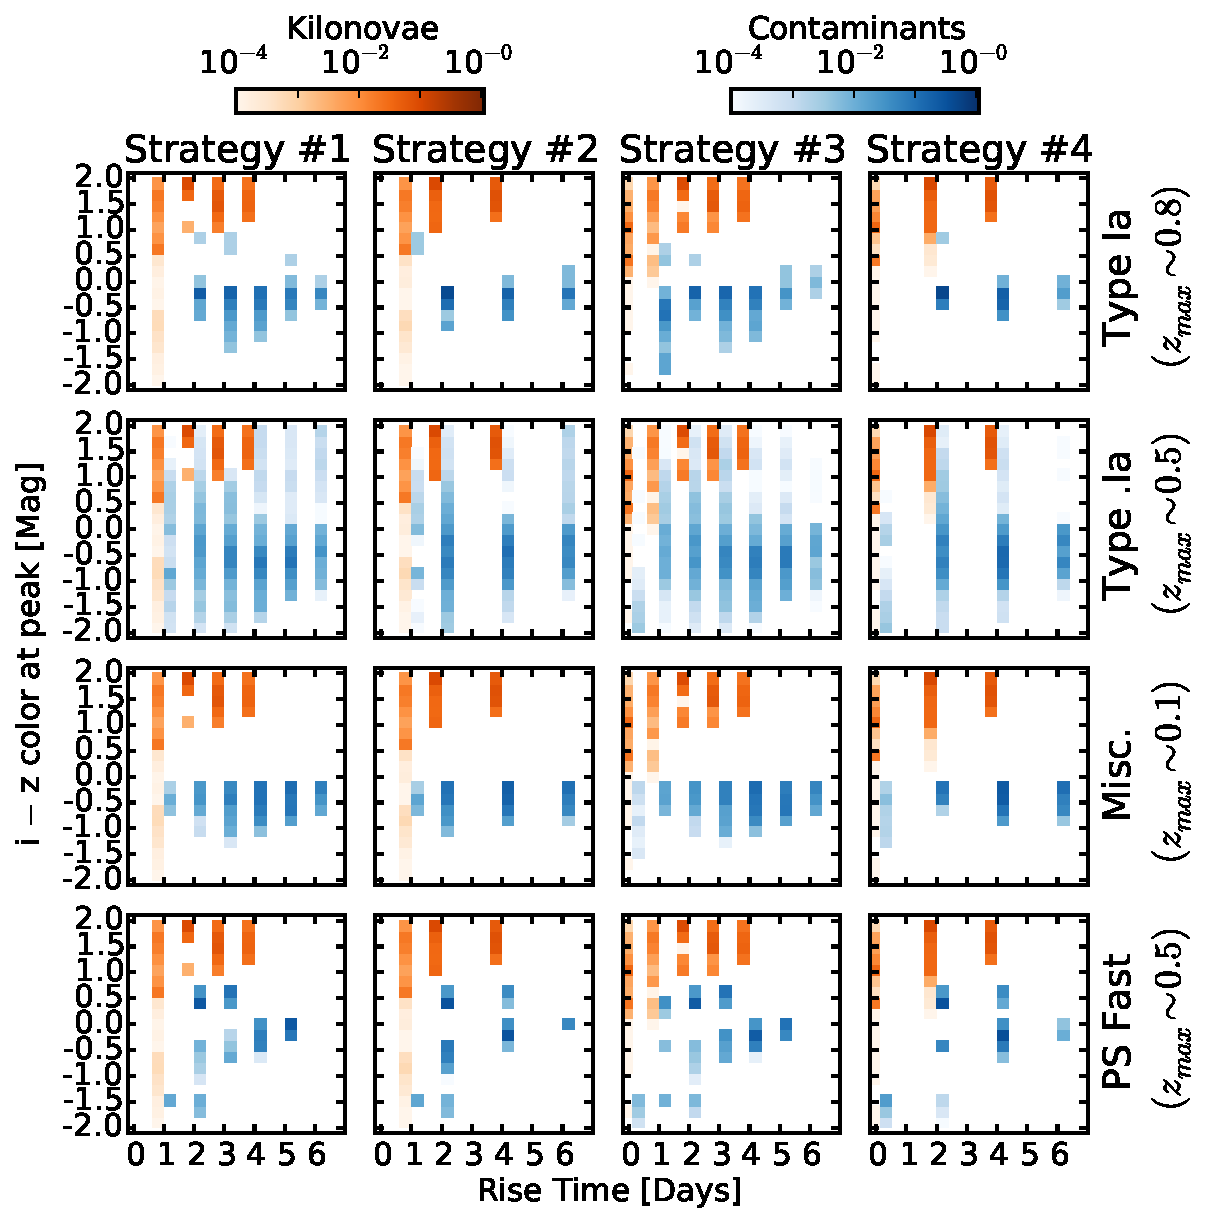
\includegraphics[width=0.9\textwidth]{./figs/chapter2/ch2_f14.pdf}
\caption{The rise time-color slice of our phase-space when a pre-existing template is not available. We note that if the rise time is long ($\gtrsim2$ days), then there is sufficient evolution in the light curve that colors can be measured with reasonable accuracy and kilonovae can be separated from the contaminants as before. However, when the rise time is short $(\sim 1$ day), then the change in flux is small and the colors are not well constrained.}
\label{fig:ch2_phaserisediff}
\end{figure}
    
In Figure~\ref{fig:ch2_phaserisediff} we plot the rise time-color slice using the same layout as in Figure~\ref{fig:ch2_mcphasecol}. Inspecting the kilonovae across all four observing strategies we note that when the observed rise time is small ($\lesssim$ 1 day, i.e. when the difference in time between the template and first science image is small) then the color is not well constrained due to $|\Delta f|$ being too small to obtain an accurate measurement. However, the fraction of kilonovae with a rise time of $\lesssim1$ day is only $\sim5-8\%$. We also note that the fraction of detected kilonovae with $t_{{\rm rise}} \lesssim 1$ day that exhibit $i-z\approx -2$ to $+0.5$ mag (i.e., in the range that overlaps with contaminants) is at most $\sim1\%$ for Strategies 3 and 4, and $\lesssim1\%$ for Strategies 1 and 2. More importantly, when the observed rise time is longer $(\gtrsim 2$ days), then $|\Delta f|$ is large enough that the $i-z$ color can be well constrained and it is generally $i-z\gtrsim1$ mag. This is consistent with the color measured when a pre-existing template is available (Figure~\ref{fig:ch2_mcphasecol}). The fraction of detected kilonovae that present a rise time of $\gtrsim 2$ days is $\sim45-55\%$. This fraction is dominated by kilonovae models with an ejecta mass of $\Mej = 10^{-1} \;M_{\odot}$ and $\beta_{\text{ej}} = $ 0.1 or 0.2.

Turning to the contaminant population, we find that several of the source classes have poorly constrained colors with some events exhibiting $i-z > 0$ mag. We can assess the impact of these contaminants by utilizing the rate data in Tables~\ref{tab:ch2_rates} and~\ref{tab:ch2_rates_Iae}. This is achieved by multiplying the expected fraction of sources in a region of the phase-space with the number of sources expected to occur during the search. This gives the actual number of sources detected. As expected, Type Ia SNe are the most numerous contaminant with $\sim3-12$ sources expected to exhibit $i-z\gtrsim0$ mag. Strategies 3 and 4 produce the fewest number of Type Ia SNe detections ($\sim 3-5$), while Strategy 2 produces the most ($\sim 12$). For the Pan-STARRS fast transients, we find that the number of sources exhibiting $i-z\gtrsim0$ mag is $\sim3$ across all four strategies. Lastly, we expect $\ll1$ type .Ia and miscellaneous fast transients to exhibit $i-z\gtrsim0$ mag. If we additionally require that the rise time is $\lesssim 4$ days the number of detected Type Ia SNe is reduced to $\sim1-7$. This does not affect the number of detected Pan-STARRS fast transients. Ultimately, we do not expect the lack of a pre-existing template to significantly hinder our ability to separate kilonovae from contaminants on the basis of their $i-z$ color and timescale, if the source is observed during the rise to peak. 

\begin{figure}[t!]
\centering
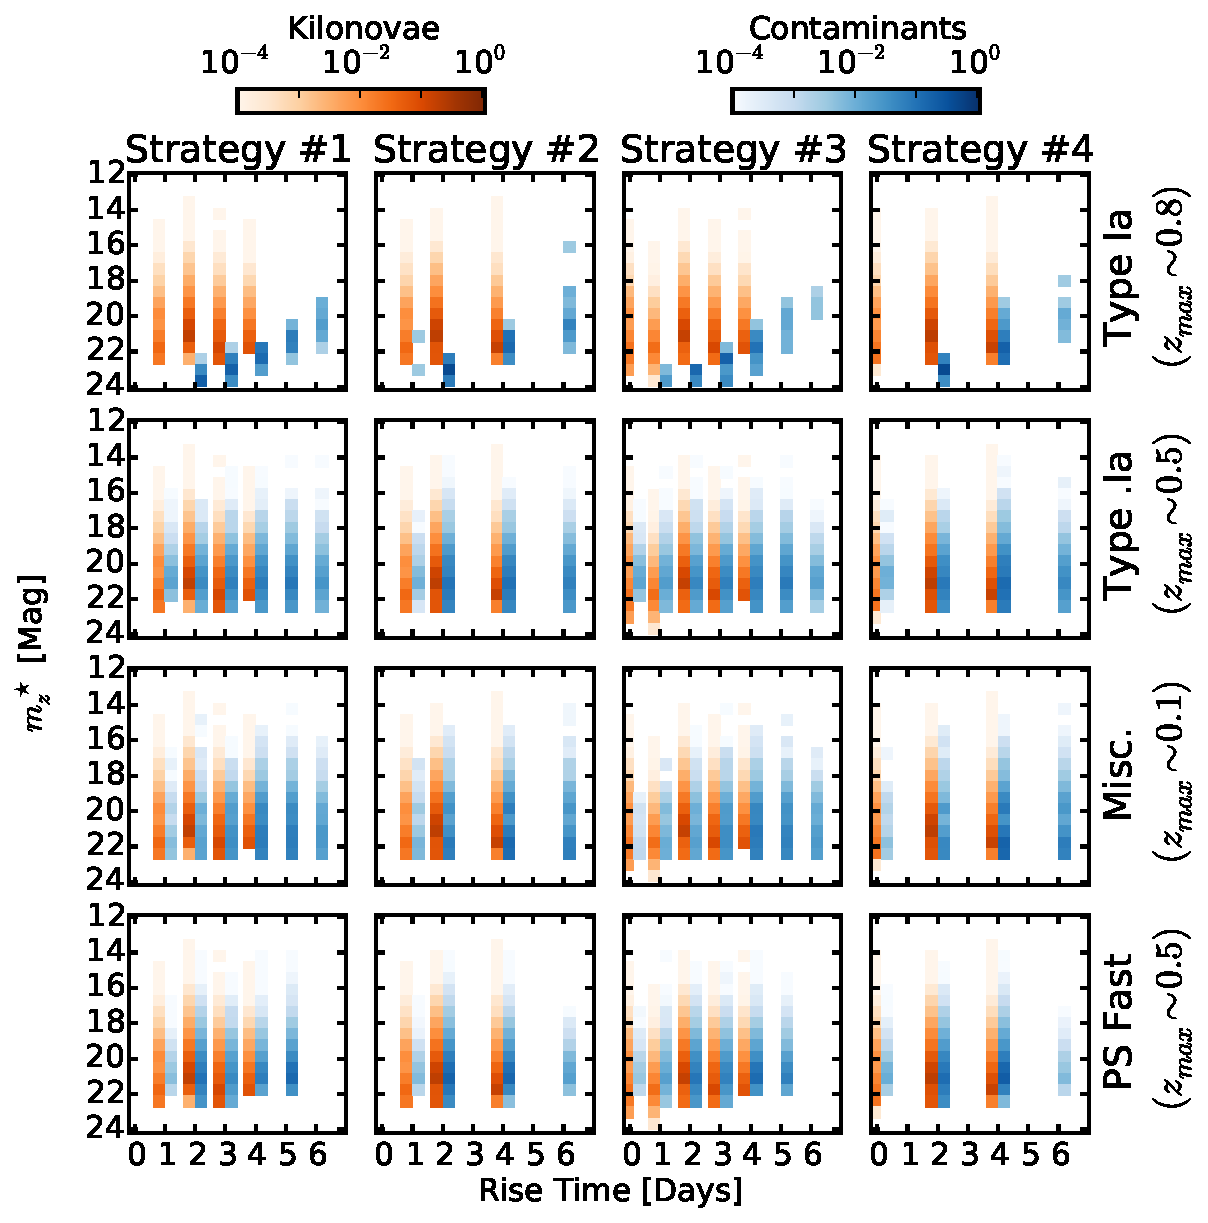
\includegraphics[width=0.9\textwidth]{./figs/chapter2/ch2_f15.pdf}
\caption{The rise time-$m^{\star}_z$ slice of our phase-space. The slower evolution of Type Ia SNe is apparent. For the remaining contaminants the observed change in flux is comparable to that observed for kilonovae. The rise times exhibited by both the kilonovae and contaminant populations are also comparable, however only contaminants show a rise time $\gtrsim 5$ days.}
\label{fig:ch2_phaserisediff_df}
\end{figure}
   
Figure~\ref{fig:ch2_phaserisediff_df} shows the rise time-$m^{\star}_z$ slice of our phase-space. We first note the wide range of values for $m^{\star}_z$ that appear in our simulations. This arises from considering contaminants over a wide redshift range or in the case of the kilonovae, over a range of model parameters. We further note that there does not appear to be an obvious cut utilizing $m^{\star}_z$ that helps to distinguish kilonovae from the contaminant population. However, we can separate kilonovae from the contaminant populations by utilizing a cut on timescale as all of the kilonovae exhibit a rise time of $\lesssim 4$ days. Therefore, if we require that sources exhibit a rise time of $\lesssim 4$ days, then we expect to eliminate $\sim 100$ Type Ia SNe, $\sim 1$ Pan-STARRS fast transient, and $\ll1$ type Ia and miscellaneous fast transients, without rejecting any kilonovae.
   
Despite the lack of a clear separation between the kilonovae and contaminant populations in $m^{\star}_z$, the requirement that sources exhibit a $m^{\star}_z$ greater than $5\sigma$ in the difference images does reduce the overall number of contaminants detected. Utilizing this criterion, the detection rates for Type Ia SNe and Pan-STARRS fast transients (the two most numerous contaminants) on the rise is $\sim1\%$ for both populations, down from $\sim60\%$ and $\sim25\%$, respectively, in the case of a pre-existing template. The downside of this approach is that $\sim10-15\%$ of kilonovae are also lost. These sources can be recovered with a late-time template, but they will not be detected in real time. 

\begin{figure}[t!]
\centering
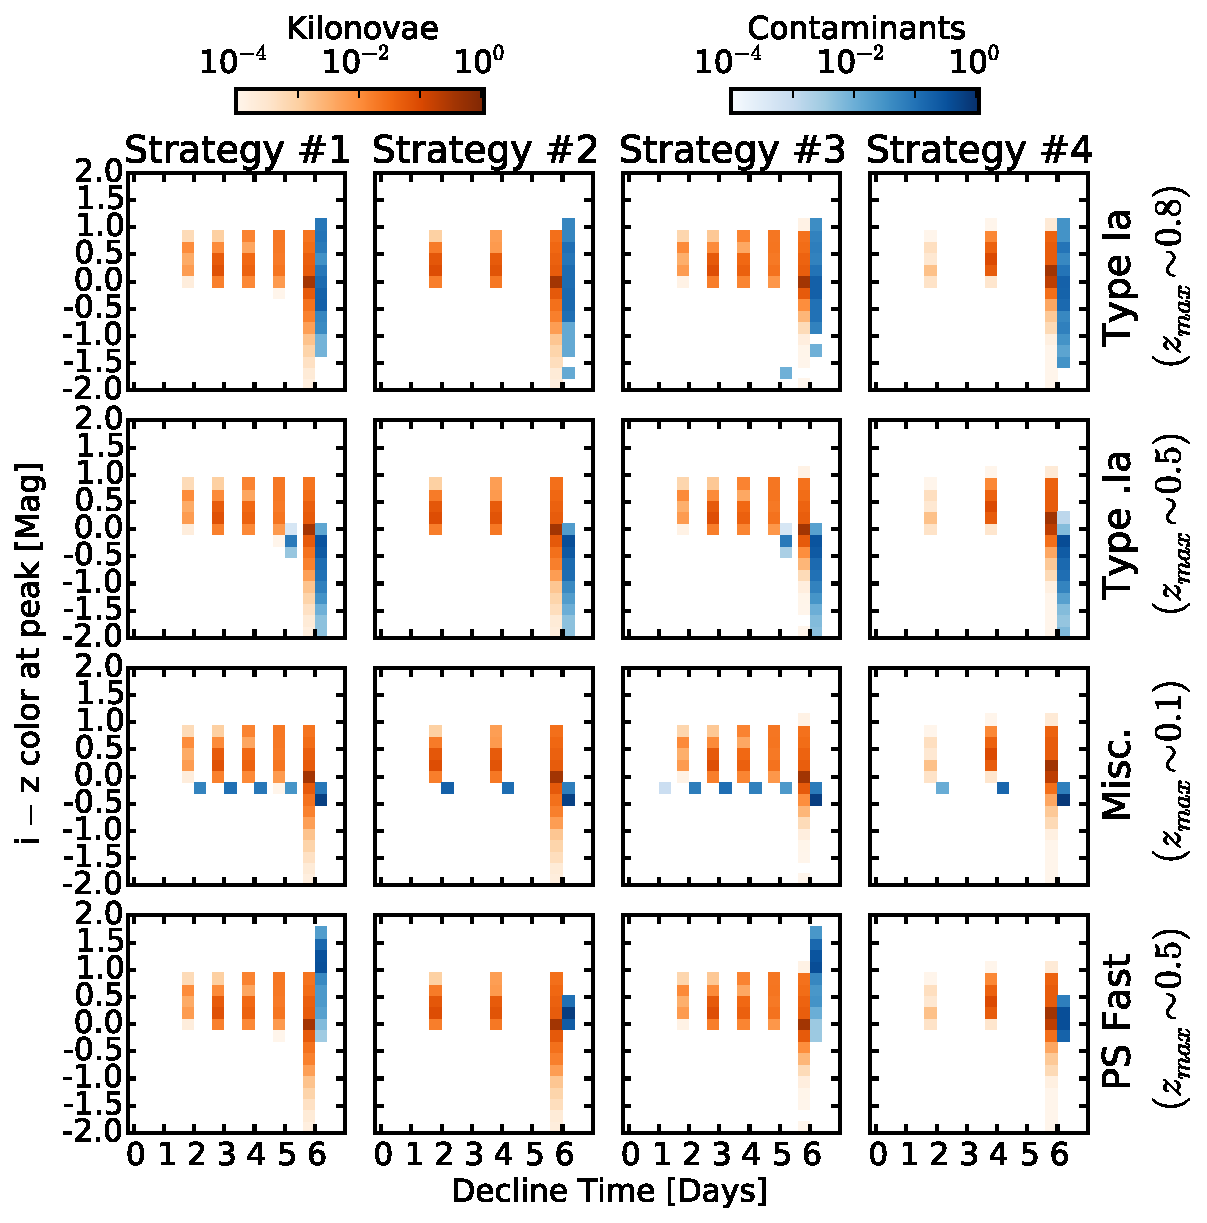
\includegraphics[width=0.9\textwidth]{./figs/chapter2/ch2_f16.pdf}
\caption{Same as Figure~\ref{fig:ch2_phaserisediff} but showing the decline time-color slice of the phase-space. The kilonovae are not always clearly separated from the contaminant population due to the imprecise color measurements. However, contaminants (with the exception of the miscellaneous fast transients) do stand out from kilonovae on the basis of their long decline times ($\gtrsim 6$ days, the maximal length given our search duration).}
\label{fig:ch2_phasedecdiff}
\end{figure}
   
In Figure~\ref{fig:ch2_phasedecdiff} we plot the decline time-color slice of our phase-space. We find that there is no longer a clear separation in color between the kilonovae and contaminant populations. This is true for all contaminants and across all observing strategies. This effect is the result of the {\em apparent} slow evolution of the light curve during the decline phase relative to the template flux. This can occur if the observations straddle the light curve peak or if the source simply evolves slower after peak. However, we can separate kilonovae from the contaminant populations by utilizing a cut on timescale as all of the contaminants predominantly exhibit a decline time of $\gtrsim 6$ days (the maximal value given the duration of our search). Therefore, if we require that sources exhibit a decline time of $\lesssim 5$ days, then we expect no Type Ia SNe, type .Ia and Pan-STARRS fast transients, and $\ll 1$ miscellaneous fast transient to be detected, but this cut will reject $\sim15-20\%$ of kilonovae.

\begin{figure}[t!]
\centering
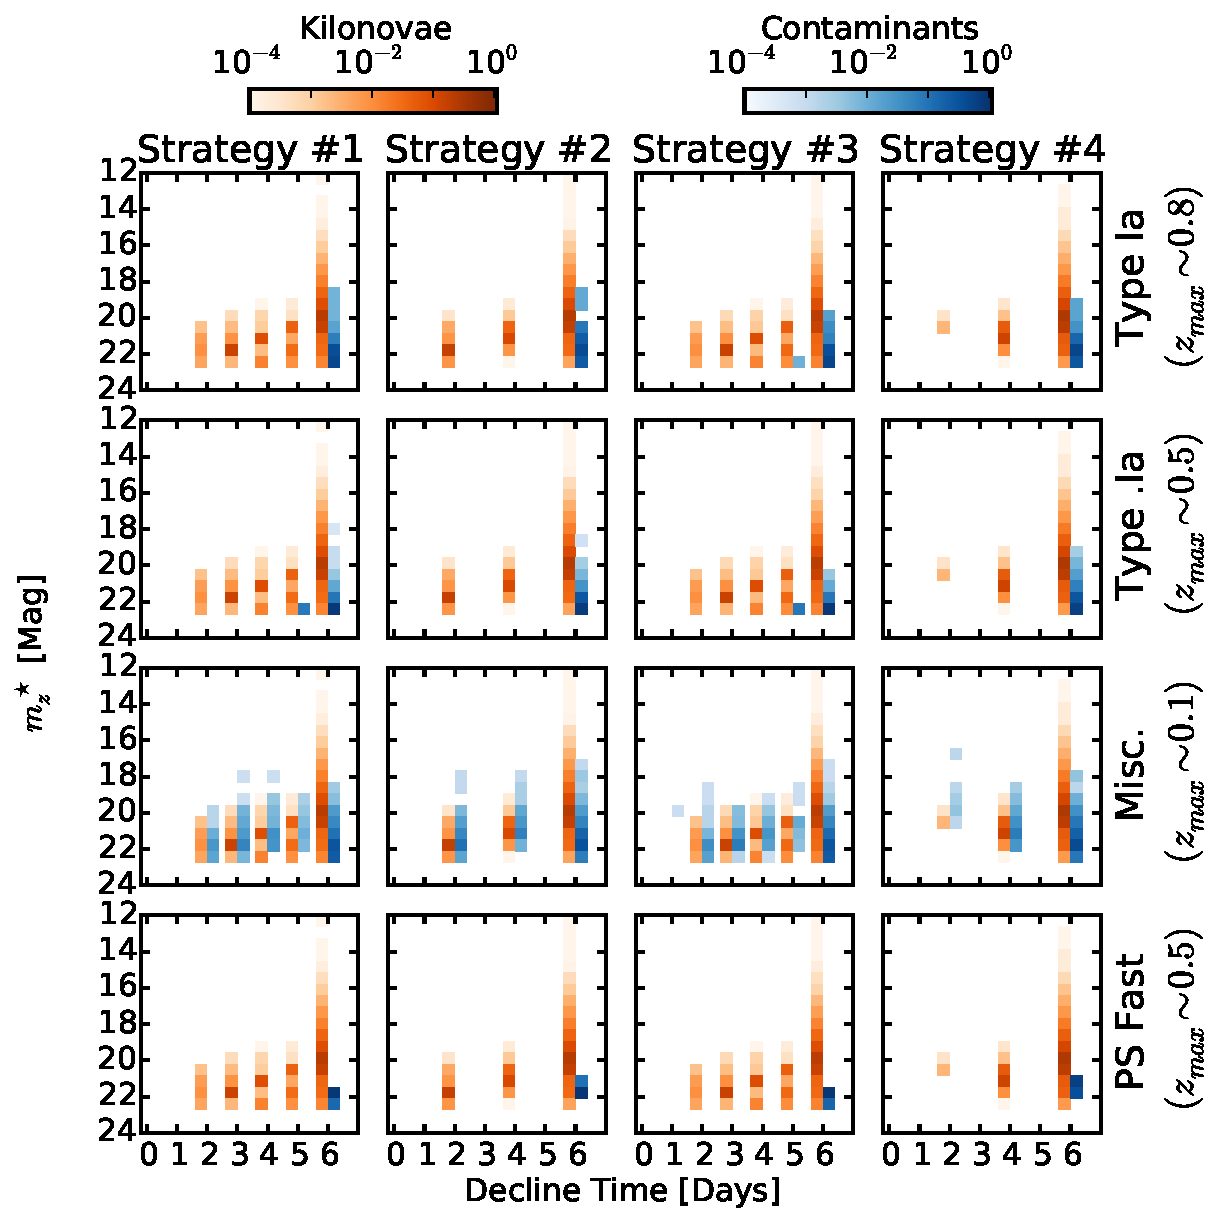
\includegraphics[width=0.9\textwidth]{./figs/chapter2/ch2_f17.pdf}
\caption{Same as Figure~\ref{fig:ch2_phaserisediff_df} but showing the decline time-$m^{\star}_z$ slice of the phase-space. As in Figure~\ref{fig:ch2_phaserisediff_df}, the contaminants are not clearly separated from the kilonovae population in $m^{\star}_z$. However, as in Figure~\ref{fig:ch2_phasedecdiff}, the long decline times can be used to distinguish kilonovae from the contaminant populations.}
\label{fig:ch2_phasedecdiff_df}
\end{figure}
   
Figure~\ref{fig:ch2_phasedecdiff_df} shows the decline time-$m^{\star}_z$ slice of the phase-space. As in the case of sources detected on the rise, there is no clear cut on $m^{\star}_z$ that will help to separate the kilonovae from any contaminants. Furthermore, a cut on decline time (e.g., $\gtrsim 6$ days) does not yield any new information beyond what is gained from the decline time-color slice of the phase-space. However, as before, utilizing a detection criterion on $m^{\star}_z$ does reduce the total number of contaminants detected. This effect is enhanced for sources such as Type Ia SNe and the Pan-STARRS fast transients, as they show slower post-peak evolution in their light curves. Here, the detection rates for these sources, when seen on the decline, is $\ll1\%$ in both cases. This is down from $\sim20\%$ and $\sim15\%$, respectively, in the case of a pre-existing template. However, the detection criterion on $m^{\star}_z$ reduces the kilonovae detection rates by $\sim5\%$. 

We now summarize the efficacy of cuts based on $i-z$ color, timescale, and change in flux for separating kilonovae from the contaminants when a pre-existing template is not available. For sources observed during the rise to peak, requiring $i-z\gtrsim0$ mag eliminates $\sim98\%$ of detected Type Ia SNe, $\sim91\%$ of detected type .Ia, $\sim100\%$ of detected miscellaneous fast transients, and $\sim 56\%$ of detected Pan-STARRS fast transients while eliminating $\lesssim0.1\%$ of detected kilonovae. If we additionally require that the rise time is $\lesssim4$ days, then we eliminate $\sim99\%$ of detected Type Ia SNe, $\sim94\%$ of detected .Ia SNe, and $\sim59\%$ of detected fast Pan-STARRS transients, without altering the fraction of kilonovae eliminated. In this scenario, an additional cut on $m^{\star}_z$ does not yield any additional information.

For sources observed only in decline, a cut of $i-z\gtrsim0$ mag eliminates $\sim50\%$ of detected Type Ia SNe, $\sim99\%$ of detected type .Ia, and $\sim 100\%$ of detected miscellaneous fast transients. The fraction of detected Pan-STARRS fast transients eliminated depends on the observing strategy; for Strategies 1 and 3 it is essentially zero, while for Strategies 2 and 4 it is $\sim11\%$ and $\sim37\%$, respectively. The reason for this variation is the fact that the different observing cadences are better matched to specific subsets of the population. The cut of $i-z\gtrsim0$ mag color also eliminates $\sim 15\%$ of detected kilonovae. If we additionally require that the decline time is $\lesssim 5$ days then we remove $\sim100\%$ of the contaminant population but also eliminate $\sim60-80\%$ of detected kilonovae. No additional information is gained from a cut on $m^{\star}_z$. Therefore, cuts on $i-z$ color and timescale are less effective when the source is observed on the decline only. This highlights the need for the rapid triggering of follow-up observations.
  
Despite these challenges, the best approach in the absence of a pre-existing template is unchanged from the results of Section~\ref{sec:ch2_MCsims_cont}. The optimal follow-up cadence is still Strategy 1, which allows good sampling of the light curve while maximizing the area that can be covered in a single night of observations. This strategy is also not subject to the dip in detection efficiency as a function of start time, seen in Strategies 2 and 4. However, we note that the previously recommended depths of 24 AB mag in {\em i}-band and 23 AB mag in {\em z}-band are only expected to detect $\sim50-75\%$ of kilonovae in this scenario (Figure~\ref{fig:ch2_detdiff}). The $i-z$ color still provides a strong constraint for separating kilonovae from contaminants but it is most reliable when the kilonova can be observed during the rise to peak. If this is not feasible due to other observational constraints, then it is best to resort to obtaining template images once the kilonova has faded in the optical ($\gtrsim$ 10 days). 

\section{Effects of Alternative Kilonovae Models}
\label{sec:ch2_altkilo}

So far, we have only considered kilonova models affected by the large opacities of r-process heavy nuclei. We now consider the effects of modifications to the standard kilonova models and their impact on our detectability results. The key issue in determining the nature of kilonova emission is the electron fraction, $Y_e$. The value of $Y_e$ in the dynamical ejecta and from accretion disk winds is low $(Y_e \lesssim 0.2)$ which leads to the production of r-process nuclei and strong suppression of the optical emission. However, if the electron fraction of the ejecta is above the critical value of $Y_e \approx 0.25$, r-process nucleosynthesis is not able to produce heavy elements \citep[particularly the lanthanides][]Kasen+15]. The resulting opacities will be closer to those from the Fe-peak elements, leading to a bluer transient. Here we investigate speculative scenarios that could produce a ``blue" kilonova component and assess their impact on {\em r}-band detectability.

\subsection{Neutrino Driven Winds}
\label{sec:ch2_neutrino}
Ejecta can be produced by the outflows from a post-merger accretion disk \citep{Dessart+09,FernandezMetzger13,Fernandez+15}. \citet{FernandezMetzger13} performed numerical two-dimensional hydrodynamical simulations of accretion disks and found that $\sim$10\% of the initial disk mass is ejected over timescales of $\sim1$ s. These ejecta are a neutron-rich wind with an electron fraction of $Y_{\text{e}} \sim 0.2$, producing conditions that are favorable for r-process nucleosynthesis. This type of outflow will therefore not drastically alter the observational properties of the kilonova. 

Recent work by \citet{Fernandez+15} found that the amount of ejected mass is a function of the spin of the remnant black hole, with more rapidly spinning black holes leading to higher ejecta masses by a factor of several. Furthermore, they found that $Y_{{\rm e}}$ increased monotonically with black hole spin due to an increased early-time neutrino luminosity from a rapidly spinning black hole. They found that in the most extreme cases $(a \gtrsim 0.8)$, the system could eject $\sim10^{-5} - 3\times10^{-3}\;M_{\odot}$ of material with $Y_{{\rm e}} \gtrsim 0.25$. Specifically, an ejecta mass of $\sim10^{-3}\;M_{\odot}$ will produce a blue component in the kilonovae light curve with $\nu L_{\nu} \approx 7.5\times10^{40}$ erg s$^{-1}$ at $\sim6500$ \AA ($r \approx 22.5$ mag at 200 Mpc) and a peak time of $\lesssim$ 1 day \citep{Kasen+15}. This is significantly brighter in $r$-band than the kilonovae models discussed previously, but the short timescales make observing this component challenging.

\subsection{A Long-Lived Hyper-massive Neutron Star}
\label{sec:ch2_HMNS}
Another modification can be caused by a  surviving hyper-massive neutron star (HMNS). The HMNS is a potential result of NS-NS mergers, but in simulations it often collapses rapidly $(t \lesssim 100$ ms) to form a black hole \citep{Sekiguchi+11}. The prompt formation of a black hole is an implicit assumption in the kilonova models discussed so far in this paper. However, if the total mass of the binary is less than a critical value, the HMNS can survive for a longer period of time \citep{Bauswein+13a,Kaplan+13}. In this scenario, the resulting neutrino luminosity will raise the electron fraction of the disk wind ejecta and will suppress r-process nucleosynthesis. Thus, the lanthanide-free disk wind material will produce a brighter, bluer, and shorter lived component in the kilonova light curve \citep[see e.g.,][and references therein]{MetzgerPiro14,MetzgerFernandez14}. This emission component will have a strong viewing angle dependence, with the polar regions being more strongly irradiated by neutrinos than the equatorial regions which will remain obscured by lanthanide-rich material. Consequently, the blue early component is more pronounced when the merger is observed along the polar axis. 

\citet{MetzgerFernandez14} found that the luminosity and timescale of this initial blue component are strongly dependent on the lifetime of the HMNS, with typical values ($\sim 100$ ms) leading to peak luminosity that is a factor of a few times brighter than the red kilonova component, with a timescale of a few days for emission along the polar direction. The light curves of this early-time component were computed in detail using wavelength-dependent radiative transfer calculations by \citet{Kasen+15}. They found that for an HMNS with a lifetime of $\sim100$ ms, the initial blue component will have a peak luminosity of $\nu L_{\nu} \approx 1.3\times10^{41}$ ergs s$^{-1}$ at $\sim6500$ \AA\,  ($r \approx 22$ mag at 200 Mpc) and a peak time of $\sim2$ days. \citet{Kasen+15} also compared the blue component to the r-process powered emission from a $10^{-2}\;M_{\odot}$ torus of dynamical ejecta. They found that the blue component will be visible for polar viewing angles $(\theta \lesssim 15$ deg). The fraction of sources expected to be observed at this viewing angle is $\sim7\theta^2\sim0.48$ \citep{MetzgerBerger12}. However, at these viewing angles the kilonova emission will be overwhelmed by the optical afterglow of an on-axis SGRB that may accompany the merger. Furthermore, if the source is observed at large viewing angles $(\theta \gtrsim 15$ deg) then the emission will become obscured by the dynamical torus and the $r$-band emission will then peak at $\gtrsim 23.7$ mag ($\sim2$ mag fainter than the polar case for a torus mass of $10^{-2}\;M_{\odot}$).
   
\subsection{A Neutron Precursor}
\label{sec:ch2_neutronpre}
Lastly, we consider the case in which a small fraction of the neutron-rich ejecta is expanding so rapidly that it avoids the initial phase of {\em r}-process nucleosynthesis. This effect has been seen in several general relativistic simulations \citep{Bauswein+13b,Goriely+14,Just+14}. In particular, \citet{Bauswein+13b} found that for a small fraction of the ejecta $(\sim 10^{-5} - 10^{-4}\; M_{\odot})$, the expansion timescale was sufficiently rapid $(\lesssim 5$ ms) that they evade neutron capture. These neutrons will undergo $\beta$-decay and release energy into the ejecta. Given that the photon diffusion time is on the order of a few hours in the outer layers of the ejecta, a significant fraction of this energy will manage to produce radiation. The light curves of this ``neutron precursor" were modeled by \citet{Metzger+15}. They found that the $\beta$-decay from the population of free neutrons at the leading edge of $10^{-4}\;M_{\odot}$ of ejecta can produce a transient with a timescale of $\sim1-2$ hours and a peak {\em r}-band magnitude of $\approx 22.2$ mag at 200 Mpc.

\begin{figure}[h!]
\centering
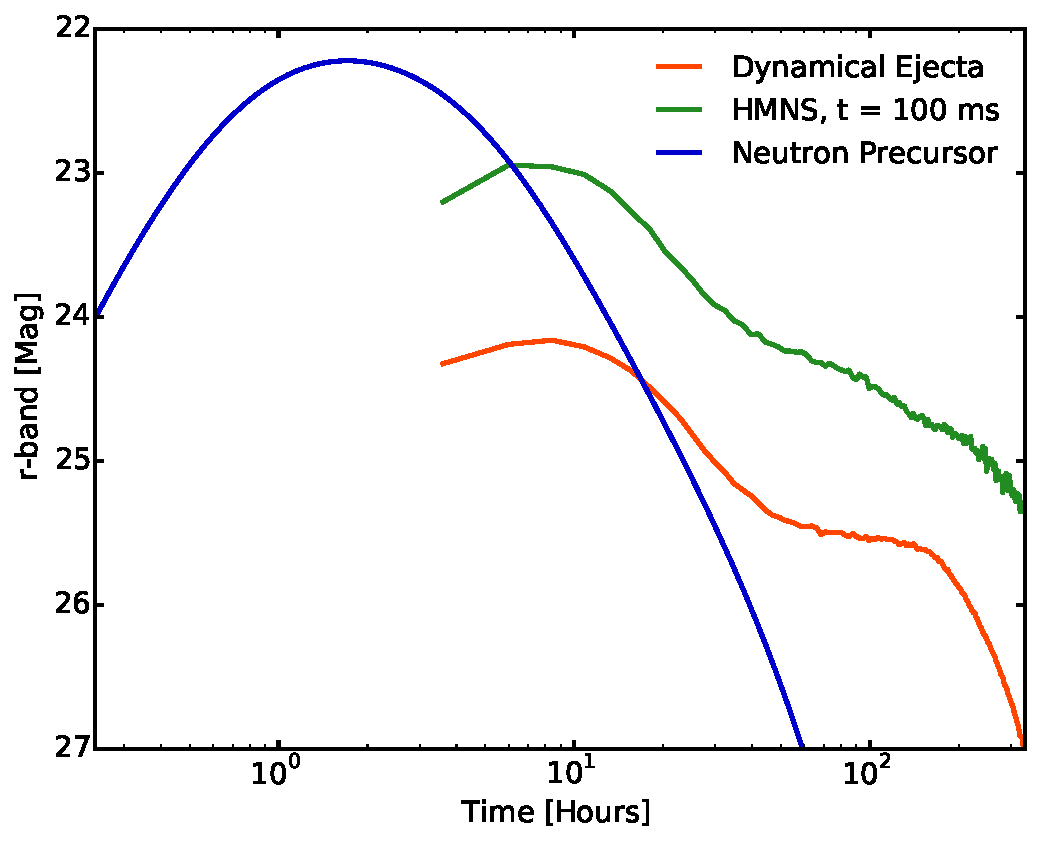
\includegraphics[width=0.9\textwidth]{./figs/chapter2/ch2_f18.pdf}
\caption{{\em r}-band light curves from the alternative kilonova models discussed in Sections~\ref{sec:ch2_HMNS} and ~\ref{sec:ch2_neutronpre}. The {\em r}-band light curve for the neutron-rich dynamical ejecta with $M_{{\rm ej}} = 10^{-2}\;M_{\odot}$ and $\beta_{{\rm ej}} = 0.2$ is plotted for comparison. The alternative models produce light curves which can be significantly brighter and bluer than the dynamical ejecta but peak at earlier times.}
\label{fig:ch2_altLC}
\end{figure}
   
\subsection{Implications for {\em r}-band detectability}
\label{sec:ch2_altkilo_det}
We now investigate the effect of these speculative models on the early-time detectability of kilonovae using {\em r}-band observations. We construct the light curves for the long-lived HMNS from the time-resolved spectra modeled by \citet{Kasen+15} using the procedure outlined in Section~\ref{sec:ch2_kilo}. These spectra are for a HMNS lifetime of 100 ms with a dynamical torus with $10^{-2}\;M_{\odot}$ of neutron-rich material observed at a viewing angle of $\cos{\theta} = 0.95\; (\theta \approx 18$ deg). For the neutron precursor, we use the {\em r}-band light curve provided by \citet{Metzger+15}, for $10^{-4}\;M_{\odot}$ of free neutrons with an electron fraction of $Y_e \approx 0.05$ and opacity of $\kappa \approx 30$ cm$^2$ g$^{-1}$. These light curves are plotted in Figure~\ref{fig:ch2_altLC} along with those from the dynamical ejecta-only model for $M_{{\rm ej}} = 10^{-2}\;M_{\odot}$ and $\beta_{{\rm ej}} = 0.2$ used in Sections~\ref{sec:ch2_MCsims} and ~\ref{sec:ch2_diff}.
   
We repeat the detectability simulations discussed in Section~\ref{sec:ch2_MCsims_det} for the two speculative light curves in Figure~\ref{fig:ch2_altLC} which are co-added in flux space to the light curve for the dynamical ejecta from \citet{BarnesKasen13}. The general simulation procedure and criteria for detection are identical to those described in Section~\ref{sec:ch2_MCsims_det}. The contours are plotted in Figure~\ref{fig:ch2_altdet}. The {\em r}-band contours for the dynamical ejecta only (Figure~\ref{fig:ch2_det}) are reproduced for comparison. 

\begin{figure}[t!]
\centering
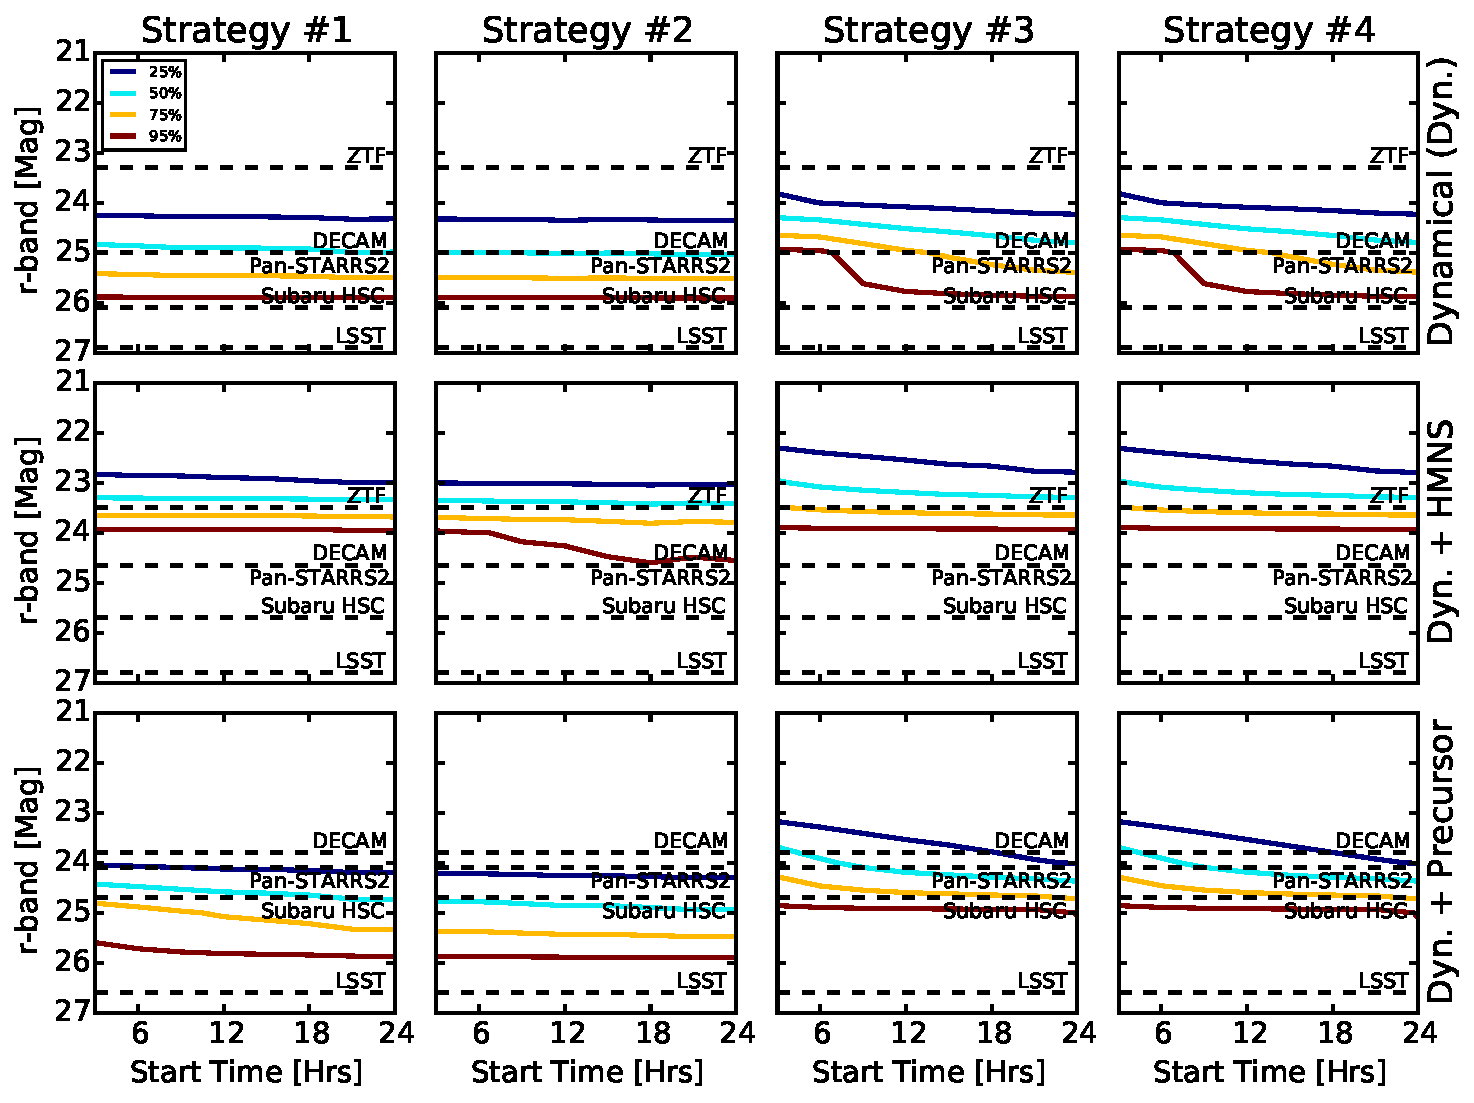
\includegraphics[width=0.9\textwidth]{./figs/chapter2/ch2_f19.pdf}
\caption{Contour plots for the {\em r}-band detectability of alternative kilonovae models. The top row shows the contours for the dynamical ejecta (reproduced from Figure~\ref{sec:ch2_MCsims_det}). The middle row shows contours for a long-lived HMNS with a lifetime of $\sim 100$ ms, surrounded by a dynamical tours with a mass of $10^{-2}\;M_{\odot}$  of neutron-rich material observed at a viewing angle of $\theta \sim 18$ deg as modeled by \citet{Kasen+15}. The bottom row shows the effect of an early-time neutron precursor as modeled by \citet{Metzger+15}.}
\label{fig:ch2_altdet}
\end{figure}
   
Inspecting the case of a long-lived HMNS, we first note that the typical depth required to detect 50\% (95\%) of events is 23.4 (24) mag across all four observing scenarios. This is shallower than the depth required for the dynamical ejecta alone, but still within reach of the larger telescopes. When a slower cadence strategy is utilized (e.g., Strategy 2 which involves observations every other night after the first observation) the 95\% detection criterion drops to 24.7 mag for observations starting more than six hours after the GW trigger. This is due to the rapid decline of the light curve after peak. Observations must then be deeper at late times to obtain the necessary three epochs for a detection. If a rapid cadence is utilized (e.g., Strategies 3 and 4), then the 50\% detection fraction contour is at 23 mag for observations within six hours of the GW trigger. The other contours are unaffected. 

For the neutron precursor model, the typical depth required to detect 50\% (95\%) of events is 24.7 (25.9) mag for observing Strategies 1 and 2, comparable to those required for the dynamical ejecta alone because the precursor is short-lived. When Strategies 3 and 4 are utilized, the 50\% detection fraction contour begins at 23.6 mag for observations starting 3 hours after the GW trigger. It then monotonically declines to 24.7 mag by 24 hours. This is again because a neutron precursor is short-lived, and only early time observations benefit from its high luminosity.

\begin{figure}[t!]
\centering
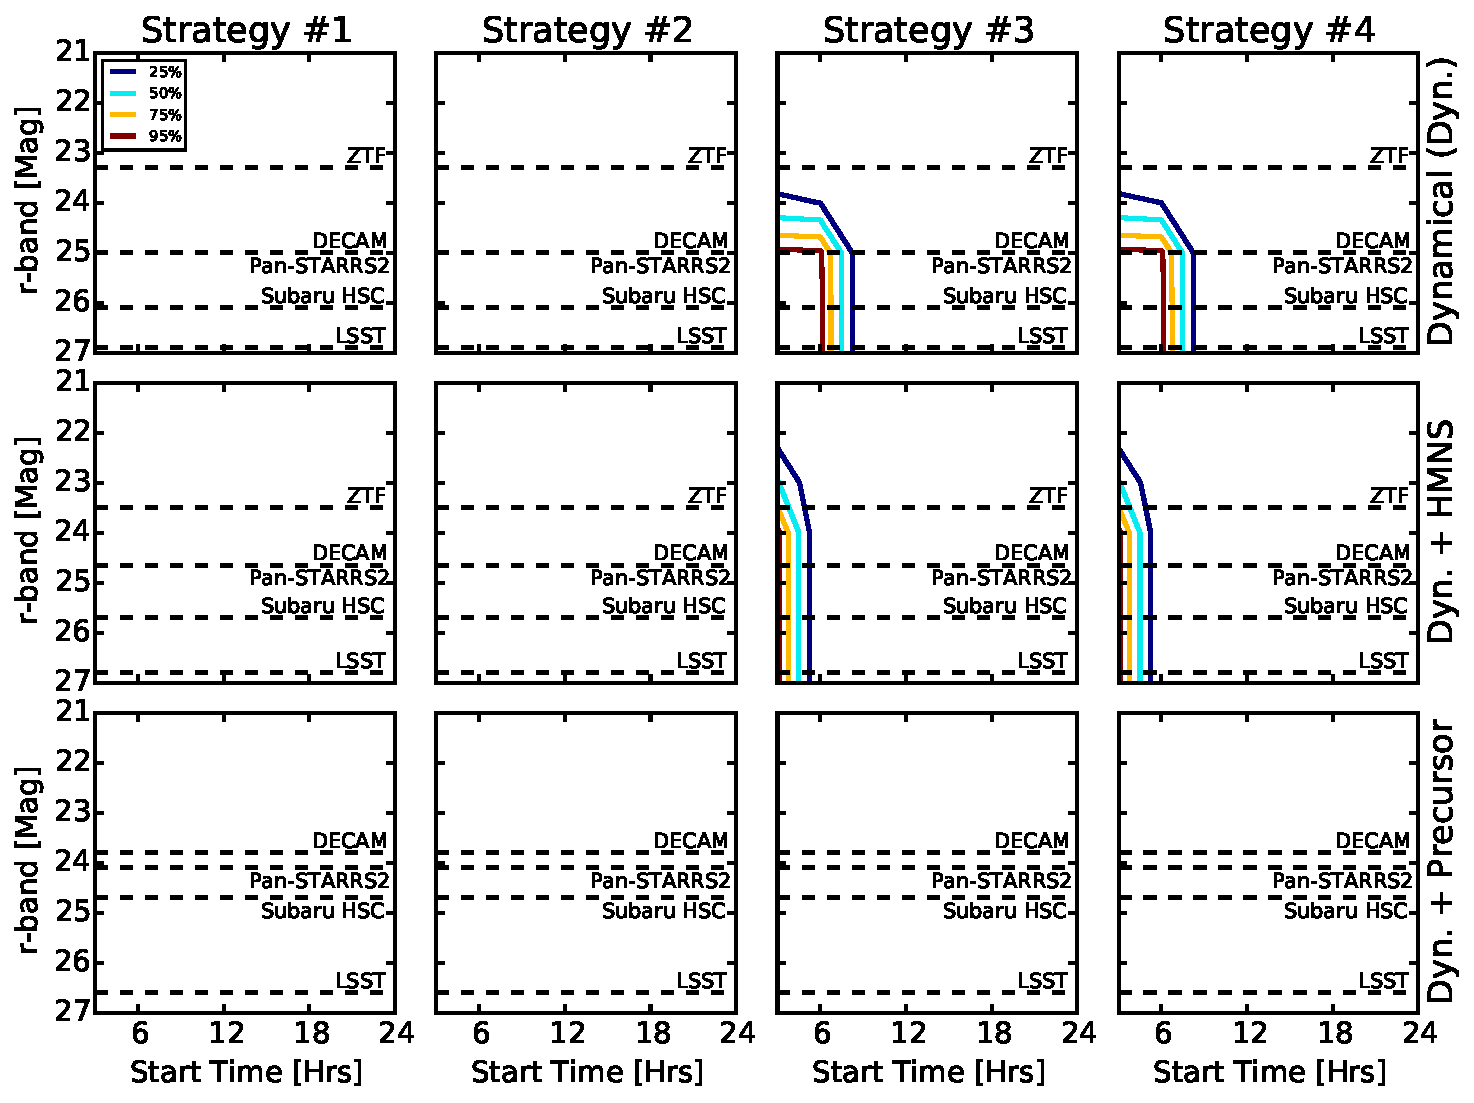
\includegraphics[width=0.9\textwidth]{./figs/chapter2/ch2_f20.pdf}
\caption{Same as Figure~\ref{fig:ch2_altdet}, but showing the fraction of events for which a brightening is detected. Compared to the case of dynamical ejecta only, it is significantly more challenging to detect brightening in these alternative kilonova models due to their earlier peak times and rapid evolution.}
\label{fig:ch2_altrise}
\end{figure}
   
Contour plots showing the detection of a rise to peak are shown in Figure~\ref{fig:ch2_altrise}. As in Section~\ref{sec:ch2_MCsims_det}, a rise is defined as any observed brightening between epochs. We note that for Strategies 1 and 2, both of which involve a single observation on the first night, the source is always seen in decline for all three models. In the case of a long-lived HMNS brightening is observed in 50\% (95\%) of events for observations starting $\lesssim5$ ($\lesssim 3)$ hours of the GW trigger and reaching a depth of $\approx$ 23 (24) mag. For a neutron precursor, brightening in the source is never observed. This is because the source peaks in $\sim$ 2 hours, while a reasonable start time is longer.
 
Ultimately, the case of a long-lived HMNS irradiating the ejecta shows the strongest potential impact on kilonova {\em r}-band detectability. However, this component has a strong dependence on viewing angle and thus will not always be observed. In addition, this component is still faint, requiring observations that achieve a depth of $\approx24$ mag in {\em r}-band to detect 95\% of the sources. This scenario is highly speculative and requires further study of the neutron star equation of state and post-merger behavior to assess the likelihood that the post-merger remnant will avoid the prompt collapse to a black hole. The scenario involving a neutron precursor does not drastically impact {\em r}-band detectability unless an observing strategies with rapid intra-night cadence is employed (i.e., a baseline of $\sim1$ hr).

\section{Follow-Up Strategies}
\label{sec:ch2_disc}
Motivated by the results of our simulated observations, we now assess the most effective methodologies for conducting efficient GW follow-up observations. There are two primary issues to address: The detection of a kilonovae, and its identification against a population of contaminant sources. Our simulations show that, in the case of a pre-existing template, observations which achieve a depth of $i\approx24$ mag and $z\approx23$ mag lead to the detection of about 95\% of kilonovae. Furthermore, observations should commence within 12 hours of the GW trigger to maximize the likelihood of detecting the source during the rise to peak. We also show that cuts made on $i-z$ color, the rise time (if available), and $\Delta m_z$ are strong discriminants for separating a kilonova from the contaminant population. Quantitatively, with $i-z\gtrsim0$ mag, a rise time of $\lesssim 4$ days, and $|\Delta m_z| \gtrsim 0.4$ mag, we can eliminate a significant fraction $(\gtrsim95\%)$ of contaminants without removing any kilonovae. If the source is seen in decline then requiring $i-z\gtrsim0$ mag and $|\Delta m_z| \gtrsim 0.4$ mag are still strong cuts, eliminating $\sim60\%$ of contaminants. If we also require a decline time of $\lesssim 5$ days then we can eliminate $\gtrsim 90\%$ of contaminants, however this cut eliminates nearly half of the kilonova population. These results do not depend strongly on the choice of cadence (i.e., there is no benefit from intra-night observations). Therefore, follow-up observations should include a single visit per filter per night for at least the first few nights following a trigger.

Taking these constraints into account; when developing the choice of observation strategy there are three questions that must be considered:
\begin{enumerate}
\item How large of an area must be covered by the observations?
\item How long is the region of interest observable? 
\item How soon after the GW trigger can observations commence?
\end{enumerate}

The first and second points are the most important considerations as the sizable localization regions from the early science-runs of Advanced LIGO present the largest observational challenge and have the most pronounced impact on the quality of data that can be obtained. The key issue here is whether or not there will be sufficient time to observe the entire GW localization region on a nightly basis. A successful GW follow-up campaign must be able to observe a significant fraction of the GW localization region in a single night to obtain the optimal cadence. The third question impacts the likelihood that we will be able to observe a kilonovae before peak. This is important as we have shown in Sections~\ref{sec:ch2_MCsims_cont} and~\ref{sec:ch2_diff} that it is easier to isolate a kilonova from the contaminant population if it is observed during the rise. Additionally, observing a kilonova at early times is important both for constraining the ejecta parameters and for testing the alternative kilonovae models outlined in Section~\ref{sec:ch2_altkilo}. Ultimately, our ability to address the three questions above depends heavily on the facilities in use.

To investigate the impact of the choice of observing facility on GW follow-up we determine the expected performance of several current and future wide-field telescopes. Specifically, we consider the performance of DECam, ZTF, Subaru Hyper Suprime-Cam (HSC), Pan-STARRS2, and LSST. We take into account the field-of-view (FoV) per pointing, the required integration time to achieve a depth of $r\approx26$, $i\approx24$, and $z\approx23$ mag, and consequently how much area can be covered per hour of observing time. We also compute the sky coverage rate when observing in $i$- and $z$-band to obtain color data. These values are given in Table~\ref{tab:ch2_tele}. 

We first look to currently available facilities (e.g., DECam, HSC, and Pan-STARRS2). In the Northern hemisphere the two available telescopes are Pan-STARRS2 and HSC. Pan-STARRS2 offers an impressive FoV ($\sim14$ deg$^2$) allowing a $\sim100$ deg$^2$ region to be imaged in just $8$ pointings. However, HSC is the clear front-runner as  the immense collecting area allows observations to achieve the target depths in much shorter integration times than Pan-STARRS2. Thus, despite the smaller FoV of HSC, the sky coverage rate for $i$- and $z$-band data is faster than Pan-STARRS2 by over a factor of two. If we consider a typical GW localization region ($\sim 100$ deg$^2$) then Pan-STARRS2 can image this region to the required $i$- and $z$-band depths in $\sim 3.5$ hours while achieving this goal with HSC will require only $\sim1.5$ hours. In the Southern hemisphere DECam is the ideal choice. The wide FoV and red-sensitive CCD of DECam allow it to quickly image a typical GW localization region. If we again consider a $\sim100$ deg$^2$  localization region, then DECam can obtain $i$- and $z$-band data at the required depths in $\sim3.5$ hours. 

We now consider future wide-field telescopes. The next major instrument to become available will be ZTF. The primary advantage of ZTF is the extremely wide FoV $(\sim47$ deg$^2$), allowing even large localization regions to be imaged in just a handful of pointings. However, the longer integration times required to achieve the target depths means that the sky coverage rate of ZTF will be slower than DECam, Pan-STARRS2, and HSC in $r$- and $i$-band. Furthermore, the lack of $z$-band capabilities makes obtaining $i-z$ color data impossible (observations in $i$-band alone may still be useful, see below). Looking further ahead, GW follow-up with LSST will be particularly effective. The large collecting area and high sensitivity allow LSST to image a GW localization region with unparalleled rapidity. If we again consider a typical localization region ($\sim 100$ deg$^2$), then ZTF will require $\sim500$ hours in $r$-band and and $\sim10$ hours in $i$-band to image the entire region to the required depths. By comparison, LSST can image the entire localization region to the required depths in $i$- and $z$-band in just $\sim10$ minutes, highlighting the immense observing power of future facilities. However, LSST is not expected to begin science operations until $\sim2022$ when GW localizations will be much improved.

While GW follow-up observations should strive to obtain $i-z$ color data as outlined above, this may not be possible because either there is insufficient time to observe the localization region in $i+z$ or because $z$-band observations are not feasible (e.g., ZTF). In this scenario, data may be taken in a single filter,  the identification of a kilonova becomes difficult. We dedicate the rest of this section to a brief discussion of eliminating contaminants when only single filter observations are possible. 

The most populous contaminant to contend with is the Type Ia SNe. In the context of observations utilizing a single filter, these contaminants are most easily eliminated by utilizing their much slower rise and decline timescales. Therefore, the best method to reject these sources is to perform image subtraction using observations that are separated by (e.g., $\gtrsim1$ day between epochs). Type Ia SNe are unlikely to be detected in these subtractions as they are unable to produce a statistically significant change in flux between the two epochs. Qualitatively, if we require a source to exhibit a change in flux of at least $|\Delta m_z| \gtrsim 0.4$ mag and a rise time of $\lesssim 4$ days, then we can eliminate $99\%$ of detected Type Ia SNe. This corresponds to $\sim6$ detected events remaining after the cuts have been applied. However, we also eliminate $\sim15-35\%$ of detected kilonova, with the higher fraction of sources eliminated in Strategies 3 and 4 where the rapid cadence of observations on the first night produces smaller values of $|\Delta m_z|$. For sources seen on the decline, if we require that the decline time is $\lesssim 5$ days and the change in flux is $|\Delta m_z| \gtrsim 0.4$, then we eliminate all of the detected Type Ia SNe, while rejecting only $\sim2\%$ of detected kilonovae. In both scenarios (e.g., sources seen to rise or only in decline) rejected kilonovae can be recovered using a late-time template image, but real time detection may be difficult. Still, despite their high expected rates, Type Ia SNe will likely prove to be one of the easiest contaminants to eliminate in GW follow-up searches. 

We can also apply the above argument to Pan-STARRS fast transients that are seen only in decline. Qualitatively, if we require that sources exhibit a decline time of $\lesssim 5$ days and a change in flux of $|\Delta m_z| \gtrsim 0.4$, then we can eliminate $\sim80\%$ of the detected Pan-STARRS fast transients, again while rejected $\sim2\%$ of the detected kilonovae. While the cuts on decline time and $|\Delta m_z|$ are not as effective here as in the case of Type Ia SNe, the lower rates ($\sim 7$ total expected during a typical GW follow-up search) means that we expect only $\sim2$ detected events to survive. These remaining sources can then be followed-up and eliminated by utilizing pointed observations as described below.

While inter-night variability is an effective tool for eliminating slowly evolving contaminants, it is not feasible for the rapidly-evolving contaminants (e.g., type .Ia, miscellaneous fast transients, and Pan-STARRS fast transients observed on the rise) as they exhibit timescales and changes in brightness comparable to those of kilonovae. We can rule out type .Ia and miscellaneous fast transients as likely contaminants by utilizing the rate information from Section~\ref{sec:ch2_rates}. We showed that the rates for such events are low, resulting in $\lesssim1$ source expected on the timescale and in the area of a typical GW follow-up campaign. We further showed in Section~\ref{sec:ch2_diff}, that if the rate information is convolved with the detection rates in our simulations, then we expect $\ll 1$ of these contaminants to appear during the course of follow-up observations. In this case, even considering the fact that the rates are poorly constrained, it is unlikely that these sources will lead to significant contamination. However, this rate argument does not apply to the Pan-STARRS fast transients as the rates of these events are sufficiently high ($\sim 7$ expected during follow-up of a typical GW error region) that they are likely to represent significant contamination. In this case, the best option is to include any such sources in a list of kilonova candidates for follow up with pointed observations as described below or wait until the source begins to decline and apply the inter-night variability arguments outlined above. 

Lastly, we consider flaring stars (e.g., M-Dwarfs, Section~\ref{sec:ch2_flarestar}) as such events are likely to become contaminants in observing strategies that rely on a single epoch to identify sources. This is particularly true for observations carried out in bluer bands (e.g., $g$ or $r$) where the flares amplitudes are larger and the kilonova timescales are much shorter. Given that flares generally exhibit short timescales \citep[minutes to hours][]{Berger+13} then if we require that a source be detected in at least two epochs separated by $\gtrsim1$ day we can efficiently eliminate all flare contaminants. The primary concern here is that rapidly evolving kilonovae (e.g., in $r$ band around peak) will also be eliminated, particularly if observations are unable to achieve a depth of $r\approx26$ mag resulting in the kilonovae only being detected in one or two epochs. Additionally, in $r$-band, the quiescent counterpart may be difficult to identify in the template images. These complications can be avoided by carrying out follow-up observations in $i$- or $z$-band.

Taking the above considerations into account, we conclude that single filter observations, particularly those conducted in $z$-band, are still viable for kilonova identification. We favor data taken in $z$-band as the shallower depths required to achieve a 95\% detection rate (when compared to the depths required to achieve a comparable detection rate in $r$- or $i$-band) allow substantially more sky area to be covered in a night of observations.  Furthermore, we have shown above that observations in $z$-band still allow robust contaminant rejection (although still less robust than when color data is available) without being susceptible to additional contamination from stellar flares as may be the case for observations in $r$- and $i$-band. We note that observational strategies that utilize a single filter are not likely to  produce a single, obvious kilonova. This may be particularly true when a pre-existing template is unavailable, reducing the efficacy of our cuts on the timescale and change in brightness. However, the strategies outlined in this section can still be utilized to generate a list of kilonova candidates. In this scenario, once a list of $\lesssim10$ candidates is generated, those sources can be further observed in the NIR and spectroscopically. NIR follow-up is crucial as kilonova are substantially redder than the other contaminants considered, with the kilonova spectrum peaking at $\sim1.5\,\mu$m. Furthermore, spectroscopic observations will allow us to look for features consistent with the production of $r$-process elements as another means of kilonova identification. These observations will vastly improve the robustness of kilonova identification and will allow us to maximize the science gained from a GW event. 

The worst-case scenario is a GW localization region that is simply too large to observe at the required depth in the available time, even in a single filter. Here, there are two possible approaches. The first is to simply obtain shallower observations at a depth that allows the entire GW localization region to be imaged. This will be useful if the source is located closer than the fiducial distance of 200 Mpc considered here, or if the ejecta mass is larger than the fiducial value of 0.01 $M_{\odot}$. However, this is risky as shallower observations are unlikely to detect the typical event. Furthermore, even if a kilonova is detected, it may only appear in one or two epochs, making it more difficult to distinguish from stellar flares. A less risky approach is to carry out the observations at the required depth, but cover the highest probability portion of the localization region, thereby maximizing the likelihood of detecting the kilonova. 

\section{Conclusions}
\label{sec:ch2_conc}
The era of gravitational wave astronomy is fast approaching, with ground-based GW interferometers expected to achieve direct detections of the inspiral and merger of compact object binaries sometime during the next few years. If we wish the maximize the science gains of these detections then the rapid identification of an EM counterpart is essential.  Observational and theoretical evidence suggests a host of potential EM counterparts spanning a wide range of timescales, luminosities, and wavelengths. Among these, the isotropic optical emission powered by the radioactive decay of $r$-process elements synthesized in the merger ejecta has proven to be a particularly enticing target. A major challenge for follow-up observations is the large sky area that needs to be observed $(\sim100\text{ deg}^2)$ combined with a substantial depth to detect a typical event. Consequently, optical searches for kilonovae will be plagued by contamination from other common transient events (e.g., Type Ia SNe) as well as from other rapidly evolving transients (e.g., see Section~\ref{sec:ch2_contaminants}). We have performed comprehensive simulations designed to probe the range of depths and cadences that may be involved in a GW follow-up campaign to determine the set of observations that will allow kilonovae detections coupled with efficient rejection of contaminants. We find that:

\begin{itemize}
\item In the case where a pre-existing template image of the target region is available (Section~\ref{sec:ch2_MCsims_det}), the optimal strategy for kilonova detection is to image the region to $i\approx 24$ and $z\approx 23$ mag with a single visit per night. We have shown that these limits are necessary to achieve a 95\% kilonova detection rate. Furthermore, observations should ideally commence within 12 hours of the GW trigger to facilitate the detection of a rise to peak in the light curve. 
\item For sources observed on the rise, cuts on $i-z$ color and rise time are effective at distinguishing kilonovae from the contaminant population (Section~\ref{sec:ch2_MCsims_cont}). Specifically, with $i-z\gtrsim0$ mag and a rise time of $\lesssim 4$ days, it is possible to eliminate $\gtrsim95\%$ of contaminants without rejecting any kilonovae. Applying the same cuts to sources seen only in decline is less effective. If we require $i-z\gtrsim0$ mag and a decline time of $\lesssim5$ days then we again eliminate $\gtrsim95\%$ of the contaminant population, but lose nearly half of the kilonovae. These rejected kilonovae can be recovered using a late-time template $(\gtrsim10$ days), but real-time kilonova identification will be hampered.
\item In the case where a pre-existing template is not available (Section~\ref{sec:ch2_diff}), we find that there is no effect on the optimal cadence, but observations must go $\sim1$ magnitude deeper than in the pre-existing template case to achieve comparable detection rates. The detection of a rise is also more difficult since the first observation must be used as a template image, reducing the amount of early-time data.
\item In the case where a pre-existing template template is not available, cuts on $i-z$ color and timescale are still effective for separating kilonovae from the contaminant population for sources observed during the rise to peak (Section~\ref{sec:ch2_diff}). However, for sources seen only in decline, these cuts are significantly less effective. We do note that by utilizing a detection criterion based on the change in brightness in an observed source we can reduce the number of contaminant sources detected. However, this also reduces the kilonovae detection rates. 
\item For the alternative kilonova models (Section~\ref{sec:ch2_altkilo}) we find that $r$-band detectability in the speculative case of a long-lives HMNS producing an early-time blue component may improve, but the short-lived nature of this component combined with the strong dependance on viewing angle means that it is not likely to be observed. If the kilonova is accompanied by a neutron precursor (Section~\ref{sec:ch2_neutronpre}), then this component will appear brighter than a kilonova ($r\approx22.2$ mag), but the extremely short timescale ($\lesssim2$ hrs) makes it unlikely to appear in follow-up observations.
\item We examine the potential of current and future wide-field telescope facilities to achieve the observational goals outlined above (Section~\ref{sec:ch2_disc}). For current facilities, we find that Subaru HSC is the best option for localization regions in the Northern hemisphere while DECam is best suited to GW follow-up in the Southern hemisphere. Both telescopes can easily image an entire GW localization region to the required depths in $i$- and $z$-band at the required cadence. In the future, GW follow-up with LSST will be particularly effective and rapid.
\item  If data in both $i$- and $z$-band cannot be obtained due to observational constraints, then an attempt at kilonova identification can be made using data from a single filter, ideally $z$-band (Section~\ref{sec:ch2_disc}). We found that without color data it is still possible to eliminate the most numerous contaminants (e.g., Type Ia SNe and Pan-STARRS fast transients) by utilizing their slow light curve evolution when compared to kilonovae. The rapidly evolving contaminants (e.g., type .Ia and miscellaneous fast transients) are not likely to be a significant contaminant on the basis of their low expected rates. Lastly, M-dwarf stellar flares are easily rejected by requiring that the source appear in at least two epochs or by identifying a quiescent counterpart in the template image.
\end{itemize}

The next step of this analysis is to test the methodologies and conclusions of this work against a set of real data. As discussed in Section~\ref{sec:ch2_intro}, we have obtained DECam $i$- and $z$-band data with the cadence and depth optimized for GW follow-up over an area of $\sim$ 70 deg$^2$. We will confront the results of this paper by using subsets of these data to mimic the four observing strategies as well as the effects of having or missing a pre-existing template (utilizing follow-up observations that we obtained about two weeks after the main survey). This will facilitate a better observational understanding of the {\em true} contaminant population on timescales relevant to GW follow-up and further refine any proposed strategies.

\begin{deluxetable}{cccccc}
\tabletypesize{\footnotesize}
\tablecolumns{6} 
\tabcolsep0.05in\footnotesize
\tablewidth{0pt} 
\tablecaption{Expected Rates For Fast Transients}
\tablehead{
\colhead{Object}&  \colhead{$\mathcal{R}_{\rm vol}$}& \colhead{$z_{\rm max}$}  &  \colhead{$\mathcal{R}_{\rm area}$} &  \colhead{$N$}     &     \colhead{Reference}      \\
\colhead{} & \colhead{(Mpc$^{-3}$ yr$^{-1}$)} & \colhead{} & \colhead{(deg$^{-2}$ yr$^{-1}$)} &  \colhead{} & \colhead{} }
\startdata
 Type .Ia    &                  10$^{-6}$                   &  0.5        &  $0.7$            &         1.4  & \citet{Bildsten+07} \\
 WD-NS mergers  &                  10$^{-5}$                   &   0.06        & $2\times10^{-2}$              &         $3\times10^{-2}$  &     \citet{Thompson2009}     \\
 WD-BH mergers  &      10$^{-5}$                   &    0.06        &   $2\times10^{-2}$              &      $3\times10^{-2}$  &    \citet{Fryer+99}          \\
AIC       &                  10$^{-6}$                   & 0.06        & $2\times10^{-3}$            &        $3\times10^{-3}$ &  \citet{Darbha+10}   \\
ELDD      &                  3$\times 10^{-7}$                   & 0.14        &    $6\times10^{-3}$           &      $1\times10^{-2}$ &  $\cdots$  \\
Pan-STARRS fast &                  5$\times 10^{-6}$                   &     0.5        &   $3.5$            &     7 &   \citet{Drout+14}  
\enddata
\tablecomments{Expected rates for the various contaminants considered in Section~\ref{sec:ch2_contaminants}. $\mathcal{R}_{\rm area}$ is computed assuming an isotropic distribution of sources in a volume defined by the comoving volume at $z_{\rm max}$.  The column $N$ refers to the number of events expected during a search covering 100 deg$^2$ for 7 days. See \S~\ref{sec:ch2_rates} or details.}
\label{tab:ch2_rates}
\end{deluxetable}

\begin{deluxetable}{cccc}
\tabletypesize{\footnotesize}
\tablecolumns{4} 
\tabcolsep0.05in\footnotesize
\tablewidth{0pt} 
\tablecaption{Expected Rates For Type Ia SNe}
\tablehead{
\colhead{Redshift}     &  \colhead{$\mathcal{R}_{\rm vol}$}&  \colhead{$\mathcal{R}_{\rm area}$}  &     \colhead{$N$} \\
\colhead{} & \colhead{(Mpc$^{-3}$ yr$^{-1}$)} &  \colhead{(deg$^{-2}$ yr$^{-1}$)} &  \colhead{} }
\startdata
0 -- 0.25 & $3\times10^{-5}$ & 3.5 & 21  \\
0.25 -- 0.50 & $4\times10^{-5}$ & 25 & 153  \\
0.5 -- 0.75 & $5\times10^{-5}$ & 65 & 394  
\enddata
\tablecomments{Expected rates for Type Ia SNe in redshift bins of $\Delta z = 0.25$ out to $z_{\rm max} = 0.75$. See \S~\ref{sec:ch2_rates}, \citet{Graur+14}, and references therein.}
\label{tab:ch2_rates_Iae}
\end{deluxetable}

\begin{deluxetable}{ccccc|cccc}
\tabletypesize{\footnotesize}
\tablecolumns{9} 
\tabcolsep0.05in\footnotesize
\tablewidth{0pt} 
\tablecaption{Required 5$\sigma$ Limiting Magnitudes for Kilonova Detection}
\tablehead{\colhead{Filter} & \multicolumn{4}{c|}{With Pre-Existing Template} & \multicolumn{4}{c}{Without Pre-Existing Template} \\
\colhead{} & \colhead{Strategy \#1} & \colhead{Strategy \#2} & \colhead{Strategy \#3} & \multicolumn{1}{c|}{Strategy \#4} & \colhead{Strategy \#1} & \colhead{Strategy \#2} & \colhead{Strategy \#3} & \colhead{Strategy \#4}}
\startdata
$r$ & 24.9 (25.9) & 25.0 (25.9) &  24.5 (25.5) & 24.5 (25.5) & 25.0 (25.9) & 25.0 (25.9) & 25.0 (25.9) & 25.1 (25.9) \\
$i$ & 23.2 (23.9) & 23.3 (24.0) & 22.9 (23.9) & 22.9 (23.9) & 24.0 (24.9) & 24.3 (25.0) & 24.0 (24.9)& 24.3 (25.0) \\
$z$ & 22.2 (22.9) & 22.4 (23.2) & 22.1 (22.9) & 22.1 (23.0) & 23.1 (23.9) & 23.2 (24.0) & 23.1 (23.9) & 23.5 (24.2) 
 \enddata
\tablecomments{\,Limiting magnitudes $(5\sigma)$ required to detect 50\% (95\%) of kilonovae as a function of observing strategy and filter (Section~\ref{sec:ch2_MCsims_det}, Figure~\ref{fig:ch2_det}). Values are averaged over all start times. We compute the required depths for follow-up observations with and without a pre-existing template (Section~\ref{sec:ch2_diff}).}
\label{tab:ch2_det}
\end{deluxetable}

\begin{deluxetable}{cccccccccc}
\tabletypesize{\footnotesize}
\tablecolumns{9} 
\tabcolsep0.05in\footnotesize
\tablewidth{0pt}  
\tablecaption{Follow-up Capabilities of Wide-Field Telescopes}
\tablehead{\multicolumn{3}{c}{} & \multicolumn{2}{c}{{\em r}-band} & \multicolumn{2}{c}{{\em i}-band} & \multicolumn{2}{c}{{\em z}-band} & \multicolumn{1}{c}{} \\
\colhead{Instrument} & \colhead{FoV} & \colhead{Etendue} & \colhead{Exp.} & \colhead{Rate}  & \colhead{Exp.}  &\colhead{Rate} & \colhead{Exp.} & \colhead{Rate} &  \colhead{$i + z$ Rate} \\
\colhead{} & \colhead{(deg$^2$)} & \colhead{(m$^2$ deg$^2$)} & \colhead{(s)} & \colhead{(deg$^2$ hr$^{-1}$)} & \colhead{(s)} & \colhead{(deg$^2$ hr$^{-1}$)} & \colhead{(s)} & \colhead{(deg$^2$ hr$^{-1}$)} &  \colhead{(deg$^2$ hr$^{-1}$)}}
\startdata
DECam$^{{\rm a}}$ & 3 &  37.7 & 4200 & 2.5 & 250 & 43 & 150 & 72 & 27  \\
ZTF$^{{\rm b}}$ & 47 & 53.2 & $9\times10^5$  & 0.2 & 1.6$\times10^4$ & 10 & {\bf --} & {\bf --}  & {\bf --}   \\
Subaru HSC$^{{\rm c}}$  & 1.8  & 90.5 & 520 & 12 & 55 & 115 & 45 & 145 & 65 \\
Pan-STARRS2$^{{\rm d}}$ & 14 & 35.6 & $1.4\times10^4$  & 4 & 700  & 72 & 350 & 144  & 30 \\
LSST$^{{\rm e}}$ & 9.6 & 315 & 390 & 88 & 28 & 1235  & 19 & 1820 & 735
\enddata
\tablecomments{Expected rates of sky coverage in deg$^2$ hr$^{-1}$ for several existing and future wide-field facilities at a depth of $r\approx26$ mag, $i\approx24$ mag and $z\approx23$ mag (i.e., the depths necessary to achieve a 95\% detection rate for kilonovae). We note that for HSC and LSST we include overhead times of 20s and 2s, respectively, as they are comparable to the exposure times. 
References: \begin{enumerate}[label=\alph*,topsep=5pt]
\item DECam ETC, \url{http://www.ctio.noao.edu/noao/content/Exposure-Time-Calculator-ETC-0}
\item \citet{Nissanke+13,Bellm2014,KasliwalNissanke14}
\item HSC ETC, \url{http://www.naoj.org/cgi-bin/img_etc.cgi}
\item Pan-STARRS DRM, \url{http://pan-starrs.ifa.hawaii.edu/}
\item LSST ETC, \url{http://dls.physics.ucdavis.edu:8080/etc4_3work/servlets/LsstEtc.html}
\end{enumerate}
}
\label{tab:ch2_tele}
\end{deluxetable}

\section*{Acknowledgments}
We thank Ryan Chornock, Maria Drout, Wen-fai Fong, Ryan Foley, Daniel Kasen, Brian Metzger, Armin Rest, and Ken Shen for helpful discussions and providing model data during the course of this analysis. P.S.C. is grateful for support provided by the NSF through the Graduate Research Fellowship Program, grant DGE1144152.

%NOTE THE LACK OF A BIBLIOGRAPHY CALL IN THIS FILE. BIBLIOGRAPHY WORK HAPPENS OUTSIDE THE CHAPTER TEX FILES.
\clearpage
%
\chapter{Chapter 3 Title}\label{c:occ2}
\chaptermark{Short Chapter 3 Title}
\begin{quote}
{\em ~~~~~~~This thesis chapter originally appeared in the literature as} \\
{authors,
{\em journal reference info}}
\end{quote}
%UNLIKE IN A REGULAR TEX FILE, DON'T PUT ANY PREAMBLE MATERIAL HERE
\clearpage
\section*{Abstract}
We present an empirical study of contamination in wide-field optical follow-up searches of gravitational wave sources from Advanced LIGO/Virgo (ALV) using dedicated observations with the Dark Energy Camera (DECam). Our search covered \apx56 deg$^2$, with two visits per night, in $i$- and $z$-band, followed by an additional set of $griz$ images three weeks later to serve as reference images for subtraction. We achieve $5\sigma$ point-source limiting magnitudes of $i \approx 23.5$ and $z \approx 22.4$ mag in the coadded single-epoch images. We conduct a search for transient objects that mimic the $i-z$ color behavior of both red ($i-z > 0.5$ mag) and blue ($i-z < 0$ mag) kilonova emission, finding 11 and 10 contaminants, respectively. Independent of color, we identify 48 transients of interest. Additionally, we leverage the rapid cadence of our observations to search for sources with characteristic timescales of $\approx1$ day and $\approx3$ hours, finding no potential contaminants. We assess the efficiency of our search with injected point sources, finding that we are 90\% (60\%) efficient when searching for red (blue) kilonova-like sources to a limiting magnitude of $i \lesssim 22.5$ mag. Using our efficiencies, we derive sky rates for kilonova contaminants of $\mathcal{R}_{\rm red} \approx 0.16$ deg$^{-2}$ and $\mathcal{R}_{\rm blue} \approx 0.80$ deg$^{-2}$. The total contamination rate is $\mathcal{R}_{\rm all} \approx 1.79$ deg$^{-2}$. We compare our results to previous optical follow-up efforts and comment on the outlook for GW follow-up searches as additional detectors (e.g., KAGRA, LIGO India) come online in the next decade.

\section{Introduction}
\label{sec:ch3_intro}
The detection of gravitational wave (GW) events during the first two observing runs of the Advanced Laser Interferometer Gravitational-Wave Observatory (aLIGO) ushered in the era of GW astronomy. The first four announced detections (GW150914, GW151226, GW170104, and GW170814) were due to binary black hole (BBH) mergers, with component masses of $\approx8-36$ M$_\odot$ \citep{LIGOGW150914,LIGOGW151226,LIGOGW170104,LIGOGW170814}.

More recently LIGO announced the first detection of gravitational waves from the inspiral and merger of a binary neutron star \citep[GW170817][]{LIGOGW170817}. This remarkable event was accompanied 1.7s later by a coincident short gamma-ray burst (SGRB) detected with the {\it Fermi} and {\it INTEGRAL} satellites \citep{LIGOGW170817grb,GW170817Fermi,Savchenko+17}. An intense follow-up effort led to the discovery of an associated optical counterpart just 11 hours post-merger \citep{LIGOMMAPaper,Arcavi+17,Coulter+17,GW170817DECam,Valenti+17}.

Initial modeling of this optical emission revealed that it was consistent expectations for a kilonova \citep{Cowp+17,Kilpatrick+17,Tanaka+17,Villar+17b, Tanaka+18}, an isotropic thermal optical/NIR transient powered by the radioactive decay of $r$-process nuclei synthesized in the merger ejecta \citep[see e.g.,][]{Metzger+10,Kasen+13,BarnesKasen13,Metzger2017}. Subsequent studies into the EM counterpart revealed the nature of the radio and X-ray emission \citep{Alexander+17,Davanzo+18,Margutti+17,Margutti+18,Mooley+18,Troja+17} and confirmed the notion of compact object mergers as the progenitors of SGRBs \citep{Fong+13, Berger2014, Fong+15, Fong+17}.

While the case of GW170817 represents a clear success and the dawn of joint GW-EM astronomy, there are many unique aspects of this discovery that should be considered. First, the source was unusually close \citep[$D \approx 40$~Mpc,][]{LIGOGW170817} with a clearly associated host galaxy \citep[NGC 4993,][]{Blanchard+17,Cantiello+18}. Furthermore, the source was unexpectedly bright at discovery \citep[$m_i \approx 17.5$~mag,][]{LIGOMMAPaper,Arcavi+17,Coulter+17,GW170817DECam,Valenti+17} making searches with 1-m class telescopes feasible. It is not clear that future detections by aLIGO will be so fortuitous or if the observed features of the kilonova associated with GW170817 will be ubiquitous. Therefore, in the context of future searches for EM counterparts, wide-field instruments on large telescopes will still be necessary to perform efficient and effect follow-up of GW sources.

For wide-field searches conducted in the optical bands, kilonovae like the one associated with GW170817 are of particular interest due to the isotropic nature of the emission and the expectation that this emission will accompany all BNS mergers, and some of the NS-BH mergers in which the NS is disrupted outside the event horizon \citep{MetzgerBerger12}. The short duration ($\lesssim {\rm week}$) and low luminosity ($L_{\rm bol} \sim {\rm a few} \times 10^{41}$~erg s$^{-1}$ at peak) of the kilonova emission make deep and rapid searches imperative. Coupled with the large search regions, this also requires the development of methodologies to robustly identify kilonovae among the vast numbers of potential contaminating sources. For example, optical follow-up of GW151226, covering hundreds of square degrees, has led to the identification of tens of unrelated transient sources despite being shallower than ideal searches for kilonova emission require \citep[e.g.,][]{GW151226PS1}. Similar wide-field efforts for GW170817 \citep[e.g., DECam][]{GW170817DECam} found 81 transients in a search covering 70 deg$^2$.

In \citet[hereafter CB15]{CowpBerger15}, we addressed the question of kilonova detectability and the associated contamination with a Monte Carlo method to simulate tens of thousands of observations of both kilonovae and potential contaminating sources (e.g., supernovae and other known and speculative rapid transients), exploring a variety of cadences and search depths. We found that nightly observations to $5\sigma$ limiting magnitudes of $i \approx 24$ and $z \approx 23$ are required to achieve a 95\% kilonova detection rate. Furthermore, the simulated observations revealed that kilonovae occupy a unique region of phase-space defined by $i-z$ color and rise time $(t_{\rm rise})$. The analysis suggests that kilonovae can be identified among contaminating sources using $i-z\gtrsim 0.3$ mag and $t_{\rm rise}\lesssim 4$ d. This motivates the need for a new and empirical investigation into the issue of contamination.

In this paper, we extend our work in \citetalias{CowpBerger15} with an empirical investigation of contamination using a set of deep, rapid-cadence observations obtained for this specific purpose with the Dark Energy Camera (DECam; \citealt{Flaugher+15}). These observations encompass four nights of data, covering 56 deg$^2$, in $i$- and $z$-bands, with two visits per night separated by $\approx 3$ hr, and a depth designed to match expected kilonova brightness within aLIGO's sensitivity volume. This dataset is unique as it targets cadences shorter than those employed by typical time-domain surveys or by any of the existing follow-up observations of aLIGO BBH merger detections, allowing direct insight into contamination in rapid searches. We use these data to conduct a search for transient sources that could mimic the $i-z$ color behavior of kilonova, considering both red ($i-z \gtrsim 0.5$~mag) and blue ($i-z \lesssim 0$~mag) scenarios.

\clearpage
The paper is organized as follows. In \cref{sec:ch3_kn_models} we describe the various kilonova models explored in this work. We present the observations and data analysis in \cref{sec:ch3_obs}. In \cref{sec:ch3_search} we discuss the methodologies and results of our search for kilonova contaminants. In \cref{sec:ch3_fakes}, we determine our search efficiency using point sources injected into the images with a wide range of brightness, fading rate, and color. In \cref{sec:ch3_contam_rates} we determine the contamination rate as a function of $i-z$ color and compare our results to those reported from optical follow-up of the current BBH merger events. We discuss the implications of our search in the context of current and future GW detectors and follow-up facilities in \cref{sec:ch3_conc}.

All magnitudes presented in this work are given in the AB system unless otherwise noted. Cosmological calculations are performed using the cosmological parameters $H_0 = 67.7$ km s$^{-1}$ Mpc$^{-1}$, $\Omega_M = 0.307$, and $\Omega_{\Lambda} = 0.691$ \citep{Planck2016}.

\section{Overview of Kilonova Models}
\label{sec:ch3_kn_models}
The mergers of compact binaries containing at least one NS are expected to produce ejecta through dynamical processes such as tidal forces and accretion disk winds \citep{Goriely+11,Bauswein+13a,Fernandez+15,Radice+16,Metzger2017}. Numerical simulations indicate that the unbound debris has a mass of $M_{\rm ej} \sim 10^{-4} - 10^{-1}$~M$_{\odot}$ with a velocity of $\beta_{\rm ej} \sim 0.1 - 0.3$, with a dependence on parameters such as the mass ratio and equation of state \citep{Hotokezaka+13,Tanaka+14,Kyutoku+15}. The ejecta are expected to be neutron rich, with a typical electron fraction of $Y_e \lesssim 0.3$, with simulations showing a range of values from $Y_e \sim 0.1 - 0.3$ \citep{Goriely+11,Bauswein+13a,Sekiguchi+15, Radice+16,SiegelMetzger17}. This electron fraction is low enough ($Y_e \lesssim 0.25$) that the ejecta are expected to undergo $r$-process nucleosynthesis, producing heavy elements $(A \gtrsim 130)$, particularly in the lanthanide and actinide groups \citep{Goriely+11,Bauswein+13a,SiegelMetzger17}. These groups of elements have open f-shells which allow a large number of possible electron configurations, resulting in a large opacity in the bluer optical bands ($\kappa_{\nu} \sim$ 100 cm$^2$ g$^{-1}$ for $\lambda \sim 1$~$\mu$m, see e.g. Figure 10 in, \citealt{Kasen+13}). A more recent calculation by \cite{Fontes+17} suggests that the lanthanide opacities may be an order of magnitude higher ($\kappa_{\nu} \sim 1000$  cm$^2$ g$^{-1}$ for $\lambda \sim 1$~$\mu$m).

Radioactive decay of the $r$-process elements synthesized during the merger heats the ejecta producing an isotropic, thermal transient \citep{LP98,Rosswog2005, Metzger+10,Tanaka+14}. The combination of low ejecta mass and high ejecta velocity, coupled with the strong optical line blanketing, results in a transient that is faint ($i \approx 23$ and $z \approx 22$ mag at 200 Mpc), red ($i-z \gtrsim 0.5$ mag), and short-lived with a typical duration of $\sim {\rm few}$ days in $z$-band and $\sim{\rm week}$ in $J$-band \citep{BarnesKasen13,Barnes+16,Metzger2017}. In the case of larger opacities \citep[e.g.,][]{Fontes+17}, the transient is expected to peak in the IR (\apx3~$\mu$m), with a duration of \apx10~days \citep{Fontes+17,Wollaeger+17}.

In addition to the neutron-rich dynamical ejecta, recent work has suggested that the mergers can also produce ejecta with a high electron fraction $(Y_e > 0.25$,  \citealt{Wanajo+14,Goriely+15}) if BNS mergers lead to a hypermassive neutron star \citep[HMNS; see e.g.,][]{Sekiguchi+11} with a lifetime of $\gtrsim 100$ ms. The resulting HMNS irradiates the disk wind ejecta with a high neutrino luminosity which raises the electron fraction of the material and suppresses $r$-process nucleosynthesis\footnote{\singlespace Even if a HMNS star is not formed, a sufficiently rapidly spinning black hole may lead to a small amount of ejecta with $Y_e \gtrsim 0.25$ \citep[see e.g.,][]{FernandezMetzger13,Fernandez+15}. In this scenario, the resulting kilonova emission is broadly identical to the HMNS case, but the lower ejecta mass leads to a faster and fainter transient.}. This material will have an opacity similar to the Fe-peak opacities seen in Type Ia SNe, producing emission that is slightly brighter ($r \approx 22$ mag at 200 Mpc), bluer ($i-z \lesssim 0$), and shorter-lived ($\approx 1-2$ days, \citealt{MetzgerFernandez14,Kasen+15}). This blue kilonova component has a strong dependence on viewing angle, with the polar regions of the ejecta being exposed to the highest neutrino flux \citep{MetzgerFernandez14,Kasen+15}. Consequently, if the merger is viewed face-on $(\theta \approx$ 15--30 deg), this blue component may be visible. We expect that up to half of mergers will be viewed at such angles \citep[see e.g.,][]{MetzgerBerger12}. However, at larger viewing angles, the lanthanide-rich material in the dynamical ejecta will obscure the blue emission, and only a red kilonova will be observed \citep{Kasen+15,Metzger2017}. While this component will be brighter than the expected $r$-band emission from the lanthanide-rich material, its detection requires rapid-cadence observations within a few hours of the GW detection (CB15).

Lastly, it has been argued that a small fraction of the merger ejecta may expand so rapidly that it is unable to undergo $r$-process nucleosynthesis \citep{Bauswein+13a}. This material instead deposits energy into the ejecta via neutron $\beta$-decay. At very early times $(\lesssim 1$ hr post merger), the specific heating rate from the neutron $\beta$-decay is an order of magnitude higher than that generated by the $r$-process nuclei \citep{Metzger2017}. This timescale is well matched to the diffusion time for the free neutron ejecta resulting in bright brief emission. For an ejecta mass with $10^{-4}$ M$_{\odot}$ of free neutrons, the resulting transient will have a peak $r$-band magnitude of $\approx 22$ mag at 200 Mpc with a characteristic timescale of $\sim 1-2$ hours \citep{Metzger+15}. This speculative early time emission is often referred to as a ``neutron precursor." However, due to the high velocity of the free neutrons $>0.4$c, this component of the ejecta may be visible before the equatorial lanthanide-rich ejecta and thus be observable for a wider range of viewing angles than the blue kilonova. This transient will be as bright as the blue kilonova emission but significantly shorter in duration requiring particularly rapid observations in response to a GW trigger \citepalias{CowpBerger15}.

To summarize, kilonova emission with red color $(i-z\gtrsim 0.5)$, a peak brightness of $z\approx22.2$~mag at 200 Mpc, and a duration of $\sim \rm few$ days is expected to be ubiquitous. Blue kilonova emission due to a surviving HMNS is expected to be bluer ($i-z \lesssim 0$~mag), similarly faint ($r \approx 22$~mag) and shorter in duration ($\lesssim 1-2$ days). This picture was confirmed by modeling of the optical emission associated with GW170817. Successfully fitting the data required models comprised of at least two components (e.g., `red' and `blue' emission) with their own distinct ejecta properties \citep{Cowp+17,Kilpatrick+17,Tanaka+17,Villar+17b, Tanaka+18}. The observed behavior and composition of the dynamical ejecta and associated red kilonova emission is robust and ubiquitous, however the nature and observability of the blue kilonova emission depends both on the fraction of cases in which a HMNS survives (unknown) and on geometrical effects ($\lesssim 50\%$).  Finally, emission due to free neutrons will be similar in brightness and color to the blue kilonova emission, but with a timescale of only $\sim \rm few$ hours; the prevalence of this signal is uncertain.  The observations described in this paper address contamination in all of these cases.

\section{Observations and Data Analysis}
\label{sec:ch3_obs}

We obtained data for this study using the DECam imager on the Blanco 4-m telescope at the Cerro Tololo Inter-American Observatory (CTIO)\footnote{\singlespace PI: Berger, \href{https://www.noao.edu/perl/abstract?2013A-0214}{NOAO 2013A-0214}}. DECam is a wide-field optical imager with a 3.3 deg$^2$ field-of-view and a CCD sensitive out to $\sim 1\mu$m \citep{Flaugher+15}, making it an ideal instrument for optical follow-up covering the sizable GW localization regions, particularly in the context of red kilonova emission. The dataset consists of 21 contiguous pointings, covering $\approx56$~deg$^2$ in the Antlia cluster,\footnote{\singlespace The effective area corresponds to 21 DECam pointings accounting for an overall $\approx 20\%$ loss of area due to chip gaps (10\%), three unused CCDs (5\%, see \cref{sec:ch3_data_cuts} and \citealt{Diehl+14}), and masked edge pixels (5\%).} with observations conducted nightly over a five day period (2013 March $1-5$ UT; ``search images''); however due to poor weather conditions the data taken on 2013 March 4 UT were unusable. Two sets of observations, separated by $\approx 3$ hours, were obtained during each observing night, with each observation consisting of two 150~s exposures in $i$-band and two 60~s exposures in $z$-band. We obtained an additional epoch for image subtraction on 2013 March 22 UT. This epoch consists of observations in $griz$-bands to determine colors for any template counterparts, with two 85~s exposures in $g$- and $r$-band, and the same exposures in $i$- and $z$-band as the initial search images. We list the central pointing coordinates for the 21 fields in \cref{tab:ch3_pointings}, and summarize the observations in \cref{tab:ch3_search,tab:ch3_templ}.

\singlespace
\begin{deluxetable}{lcc}
\tabletypesize{\footnotesize}
\tablecolumns{3}
\tablewidth{0pt}
\captionsetup{justification=centering}
\tablecaption{Field Pointing Centers
\label{tab:ch3_pointings}}
\tablehead{
    \colhead{Pointing} &
    \colhead{R.A.} &
    \colhead{Decl.}}
\startdata
Antlia 1 & 10:19:58.5  & $-$30:55:24 \\
Antlia 2 & 10:19:44.5  & $-$33:07:24 \\
Antlia 3 & 10:19:30.5  & $-$35:19:24 \\
Antlia 4 & 10:19:10.5  & $-$37:31:24 \\
Antlia 5 & 10:30:03.5  & $-$30:55:24 \\
Antlia 6 & 10:30:03.5  & $-$33:07:24 \\
Antlia 7 & 10:30:03.5  & $-$35:19:24 \\
Antlia 8 & 10:30:03.5  & $-$37:31:24 \\
Antlia 9 & 10:40:08.5  & $-$30:55:24 \\
Antlia 10 & 10:40:22.5  & $-$33:07:24 \\
Antlia 11 & 10:40:38.5  & $-$35:19:24 \\
Antlia 12 & 10:40:57.5  & $-$37:31:24 \\
Antlia 13 & 10:50:12.5  & $-$30:55:24 \\
Antlia 14 & 10:50:41.5  & $-$33:07:24 \\
Antlia 15 & 10:51:13.5  & $-$35:19:24 \\
Antlia 16 & 10:51:50.5  & $-$37:31:24 \\
Antlia 17 & 11:00:17.5  & $-$30:55:24 \\
Antlia 18 & 11:01:00.5  & $-$33:07:24 \\
Antlia 19 & 11:01:48.5  & $-$35:19:24 \\
Antlia 20 & 11:02:44.5  & $-$37:31:24 \\
Antlia 21 & 10:36:36.0  & $-$27:31:04 \\
\enddata
\tablecomments{Central J2000 coordinates for all 21 fields used in this analysis.}
\end{deluxetable}

\begin{deluxetable}{lcrcccccc}
\tabletypesize{\footnotesize}
\tablecolumns{9}
\tablewidth{0pt}
\tablecaption{Summary of Search Observations
\label{tab:ch3_search}}
\tablehead{
    \colhead{Night}    &
    \colhead{Epoch} &
    \colhead{UT}       &
    \colhead{$\langle$PSF$_i$$\rangle$}    &
    \colhead{$\langle$PSF$_z$$\rangle$}    &
    \colhead{$\langle$airmass$\rangle$}  &
    \colhead{$\langle$depth$_i\rangle$}   &
    \colhead{$\langle$depth$_z\rangle$} \\
    \colhead{ } &
    \colhead{ } &
    \colhead{ } &
    \colhead{(arcsec)} &
    \colhead{(arcsec)} &
    \colhead{ } &
    \colhead{(mag)} &
    \colhead{(mag)}
}
\startdata
	1 & A & 2013-03-01 & 0.92 & 0.86 & 1.20 & 23.2 & 22.3 \\
           & B & 2013-03-01 & 1.01 & 0.97 & 1.03 & 23.2 & 22.4 \\
	%\hline
  	2 & A & 2013-03-02 & 1.08 & 1.05 & 1.22 & 23.2 & 22.1 \\
           & B & 2013-03-02 & 1.09 & 1.06 & 1.03 & 23.4 & 22.3 \\
  	%\hline
  	3 & A & 2013-03-03 & 0.90 & 0.87 & 1.13 & 23.6 & 22.4 \\
            & B & 2013-03-03 & 0.91 & 0.87 & 1.03 & 23.6 & 22.5 \\
 	%\hline
  	4 & A & 2013-03-05 & 0.87 & 0.82 & 1.15 & 23.7 & 22.5 \\
           & B & 2013-03-05 & 0.92 & 0.89 & 1.07 & 23.7 & 22.6 \\
\enddata
\tablecomments{Summary of our DECam observations used as search epochs. The data taken on 2013 March 4 UT are omitted as they are unusable due to poor weather conditions. The PSF and airmass are averaged across all observations on a given date. The $5\sigma$ point source depth is the mean value computed for the coadded search images.}
\end{deluxetable}

\begin{deluxetable}{lcccc}
\tabletypesize{\footnotesize}
\tablecolumns{5}
\tablewidth{0pt}
\tablecaption{Summary of Template Observations
\label{tab:ch3_templ}}
\tablehead{
    \colhead{Filter} &
    \colhead{$\langle$PSF$\rangle$}    &
    \colhead{$\langle$airmass$\rangle$}  &
    \colhead{$\langle$depth$\rangle$} \\
    \colhead{ } &
    \colhead{(arcsec)} &
    \colhead{ } &
    \colhead{(mag)}
}
\startdata
$g$-band & 1.03 & 1.07 & 22.8 \\
$r$-band & 0.95 & 1.08 & 23.0 \\
$i$-band & 0.90 & 1.09 & 23.2 \\
$z$-band & 0.87 & 1.09 & 22.1 \\
\enddata
\tablecomments{Summary of our DECam observations used for the
template epoch. All data were taken on 2013 March 22 UT. Values
are computed as for \cref{tab:ch3_search}}
\end{deluxetable}
\doublespace

\clearpage
We processed the data using {\tt photpipe}, an image processing pipeline used by several previous time domain surveys (see e.g., \citealt{Rest+05,Rest+14}) to perform single-epoch image processing, image subtraction, and candidate identification. The single epoch processing began with the raw images and appropriate calibration files obtained from the NOAO archive\footnote{\singlespace \url{http://archive.noao.edu/}} and initial image reduction (e.g., bias subtraction, cross-talk corrections, flat-fielding). We performed astrometric calibration relative to the 2MASS $J$-band point-source catalog. Search and template images were deprojected into a tangential plane and pairs of $i$- and $z$- band images from a single epoch were coadded using {\tt SWARP} \citep{Bertin+02}.

We performed photometric calibration using the PS1 3$\pi$ survey to compute zeropoints for SDSS Stripe~82 standard images taken on each observing night. We applied appropriate corrections between PS1 and DECam magnitudes to these zeropoints \citep{Scolnic+15}. We propagated the corrected zeropoints to the science observations with appropriate scaling for exposure time and airmass.

We then performed image subtraction using the 2013 March 22 UT observations as template images. Difference imaging was performed in {\tt photpipe} using the {\tt hotpants} software package \citep{Alard2000,Becker2015}. Source detection and point spread function (PSF) photometry was performed on the subtracted images using an implementation of {\tt DoPhot} \citep{Schechter+93} that has been optimized for difference images.

\clearpage
In addition to the photometry performed by {\tt photpipe}, we also constructed secondary catalogs for all sources identified in the $griz$-band template epochs. This was accomplished using the {\tt Source Extractor} ({\tt SExtractor}) photometry package in single-image mode \citep{BertinArnouts96}. We also performed forced aperture photometry in the template epoch at the position of each candidate identified by {\tt photpipe}. This approach helps to identify the presence of flux in the template images for objects not detected by {\tt SExtractor} which is indicative of image artifacts and defects. We use these additional template catalogs as a useful tool for candidate classification and artifact rejection (see \cref{sec:ch3_source_cuts}).

Our search images achieve an average 5$\sigma$ depth of $i \approx 23.5$ and $z \approx 22.4$~mag for point-sources in the coadded single-epoch images (\cref{tab:ch3_search}). The coadded template images achieve a $5\sigma$ depth for point-sources of $g \approx 22.8$, $r \approx 23.0$, $i \approx 23.2$ and $z \approx 22.1$~mag (\cref{tab:ch3_templ}). The estimated average 5$\sigma$ limiting magnitudes for point sources in the difference images are $i \approx 23.2$ and $z \approx 22.3$ mag (see \cref{sec:ch3_fakes}). There is a mean scatter in the $5\sigma$ depths in the search and difference images of $\approx 0.2$~mag between epochs.

\clearpage
\section{A Search for Optical Transients}
\label{sec:ch3_search}

Our primary goal is to uncover all optical transients in our data and then to determine specifically the areal rate of kilonova contaminants.

\subsection{Selection Based On Data Quality and Fading Behavior}
\label{sec:ch3_data_cuts}

Our initial selection criteria are designed to identify transient sources in our search images that have sufficient data quality for further analysis. These selection criteria are:

\begin{enumerate}
\item Given that we are simulating follow-up triggered by a GW detection, we search for sources that are detected at the beginning of our search (i.e., we treat our first night of observations as if it followed a GW detection notice). We accomplish this by requiring four $5\sigma$ detections in any combination of $i$- or $z$-band across the first four epochs (i.e., four total detections across the first two nights).  This selection criterion leads to an initial sample size of 2818 sources.

\item We expect both kilonovae and any relevant contaminating source in the context of GW follow-up, to be fainter in the template image than in the search images. Therefore, we only select sources that present a difference flux that is strictly positive or within $2\sigma$ of zero across all epochs. This selection criterion leads to a final sample size of 929 sources\footnote{\singlespace To check for bias from our initial selection, we also identified sources that exhibit strictly negative difference fluxes finding a comparable number (1107 sources).}.
\end{enumerate}

\clearpage
We note that at the time these data were taken CCD \#61 (N30) was not functioning. Additionally, during processing of the candidate list we observed severe data quality issues with CCDs \#16 (S17) and \#44 (N13) that produced a number of image artifacts and erroneous detections several orders of magnitude larger than in the other CCDs. Consequently, these three CCDs have been excluded from the analysis. This results in a $\approx 5\%$ loss of sky coverage as discussed in \cref{tab:ch3_search}.

\subsection{Selection Based On Template Counterpart}
\label{sec:ch3_source_cuts}

We now discuss selection criteria designed to eliminate sources that do not exhibit temporal evolution and colors expected for kilonovae. Specifically, we first leverage the fact that kilonovae are expected to have much shorter durations than most other contaminating sources (CB15). For example, a kilonova following the model of \citealt{BarnesKasen13} will fade by several magnitudes over the course of a few days, independent of the precise choice of ejecta parameters. Given that the separation in time between our last search epoch and our template epoch is 17 days, we therefore expect any kilonova-like source detected in the search images to have faded well below our detection limit in the template epoch.

Following this reasoning, we separate our population of 929 candidates into four sub-groups based on the presence and morphology (i.e., point versus extended source) of a counterpart source in the template images. We identify such counterparts (or lack thereof) by matching the detection coordinates in our difference images against those sources detected in the {\tt SExtractor} catalogs (\cref{sec:ch3_obs}). We define four sub-groups of the 929 sources in the following manner:

\begin{enumerate}
\item The candidate has no counterpart detection in the template epoch within a matching radius of $3\arcsec$.

\item The candidate has an extended source counterpart in the template epoch within a matching radius of $3 \arcsec$.

\item The candidate has a point source counterpart in the template epoch within a matching radius of $1\arcsec$, as well as an extended source counterpart brighter than 17.5 mag within a matching radius of $30\arcsec$.

\item The candidate has a point source counterpart in the template epoch within a matching radius of $1\arcsec$, without an extended source counterpart brighter than 17.5 mag  within a matching radius of $30\arcsec$.
\end{enumerate}

The choice of a $3\arcsec$ matching radius for Groups 1 and 2 is arbitrary, but does not ultimately affect the identification of candidates; changing the matching radius will simply shift candidates between Group 1 and Group 2.

In Groups 3 and 4, the choice of galaxy brightness and matching radius are motivated by observations of the host galaxies of Short GRBs, which have luminosities of $\gtrsim 0.1$ L$^\star$ \citep{FongBerger13,Fong+13,Berger2014}. At the ALV design-sensitivity detection range $(\sim 200$ Mpc) such galaxies will be brighter than 17.5 mag.

\clearpage
We then select the matching radius such that the probability of the point source and galaxy being associated by chance, the ``probability of chance coincidence", is $P_{\rm cc}\lesssim 0.1$. This is given by:

\begin{equation}
P_{\rm cc}(<R) = 1 - \exp{[-\pi R^2 \sigma(<m)]},
\end{equation}

\noindent where

\begin{equation}
\sigma(<m) = \left ( \frac{1}{0.33 \ln(10)} \right ) \times 10^{0.33(m - 24) - 2.44} \; {\rm arcsec}^{-2},
\end{equation}

\noindent is the expected number density of galaxies brighter than magnitude $m$ as determined by deep optical surveys (\citealt{Berger2010}, see also \citealt{Hogg+97,Bloom+02,Beckwith+06}). Therefore, setting $m = 17.5$ mag and $P_{\rm cc}(<R) = 0.1$, we find the appropriate matching radius of $R = 30\arcsec$. This radius, corresponding to a physical scale of $\approx 27$~kpc at a distance of $\approx200$~Mpc, also corresponds to some of the larger offsets measured for SGRB \citep{Fong+10,FongBerger13,Berger2014}.

\subsubsection{Group 1 -- No Counterpart}
\label{sec:ch3_group1}

The first group is designed to identify sources that were detected during our search epochs but have faded below our detection threshold by the time of the template observations. Here, the matching radius $(3 \arcsec)$ is chosen such that this group of candidates will serve as the complement to the second group, as discussed above. We find that 110 of our original 929 sources belong to Group 1, but 63 of these 110 sources exhibit a $\gtrsim 3 \sigma$ detection in forced aperture photometry in the template images indicating the presence of artifacts (e.g., diffraction spikes caused by saturated stars), that are unidentified by {\tt SExtractor}. This reduces the number of candidates to 47. Manual inspection reveals these to also be image defects, specifically bad CCD columns and fringing artifacts. We therefore find no genuine transient sources that have faded beyond the limits of our template images and which have no counterparts within $3\arcsec$.

\subsubsection{Group 2 -- Extended Source Counterpart}
\label{sec:ch3_group2}
We next search for transients that appear near to a galaxy, but like those in Group 1, have faded below the detection limit of our template epoch. We identify extended sources as those detected by {\tt SExtractor} with a {\tt CLASS\_STAR} (i.e., stellarity) value of $\le 0.8$. Applying this cut, we find that this subsample contains 94 of the original 929 sources. Visual inspection reveals that 48 of these sources are genuine transients (which we consider as potential kilonova contaminants), while the remaining 46 sources result from image subtraction artifacts in the cores of bright galaxies; we do not consider these sources in the analysis. The distribution of offsets between the transients and galaxies for the sample of 48 genuine sources is shown in \Cref{fig:ch3_offset_hist}. We find that that half (24 of 48) of the sources have an offset of $\lesssim 0.27\arcsec$ (i.e., one DECam pixel), hinting that they are nuclear in origin, and hence likely represent AGN variability.

\begin{figure}[!t]
\begin{center}
\hspace*{-0.1in}
\scalebox{1.}
{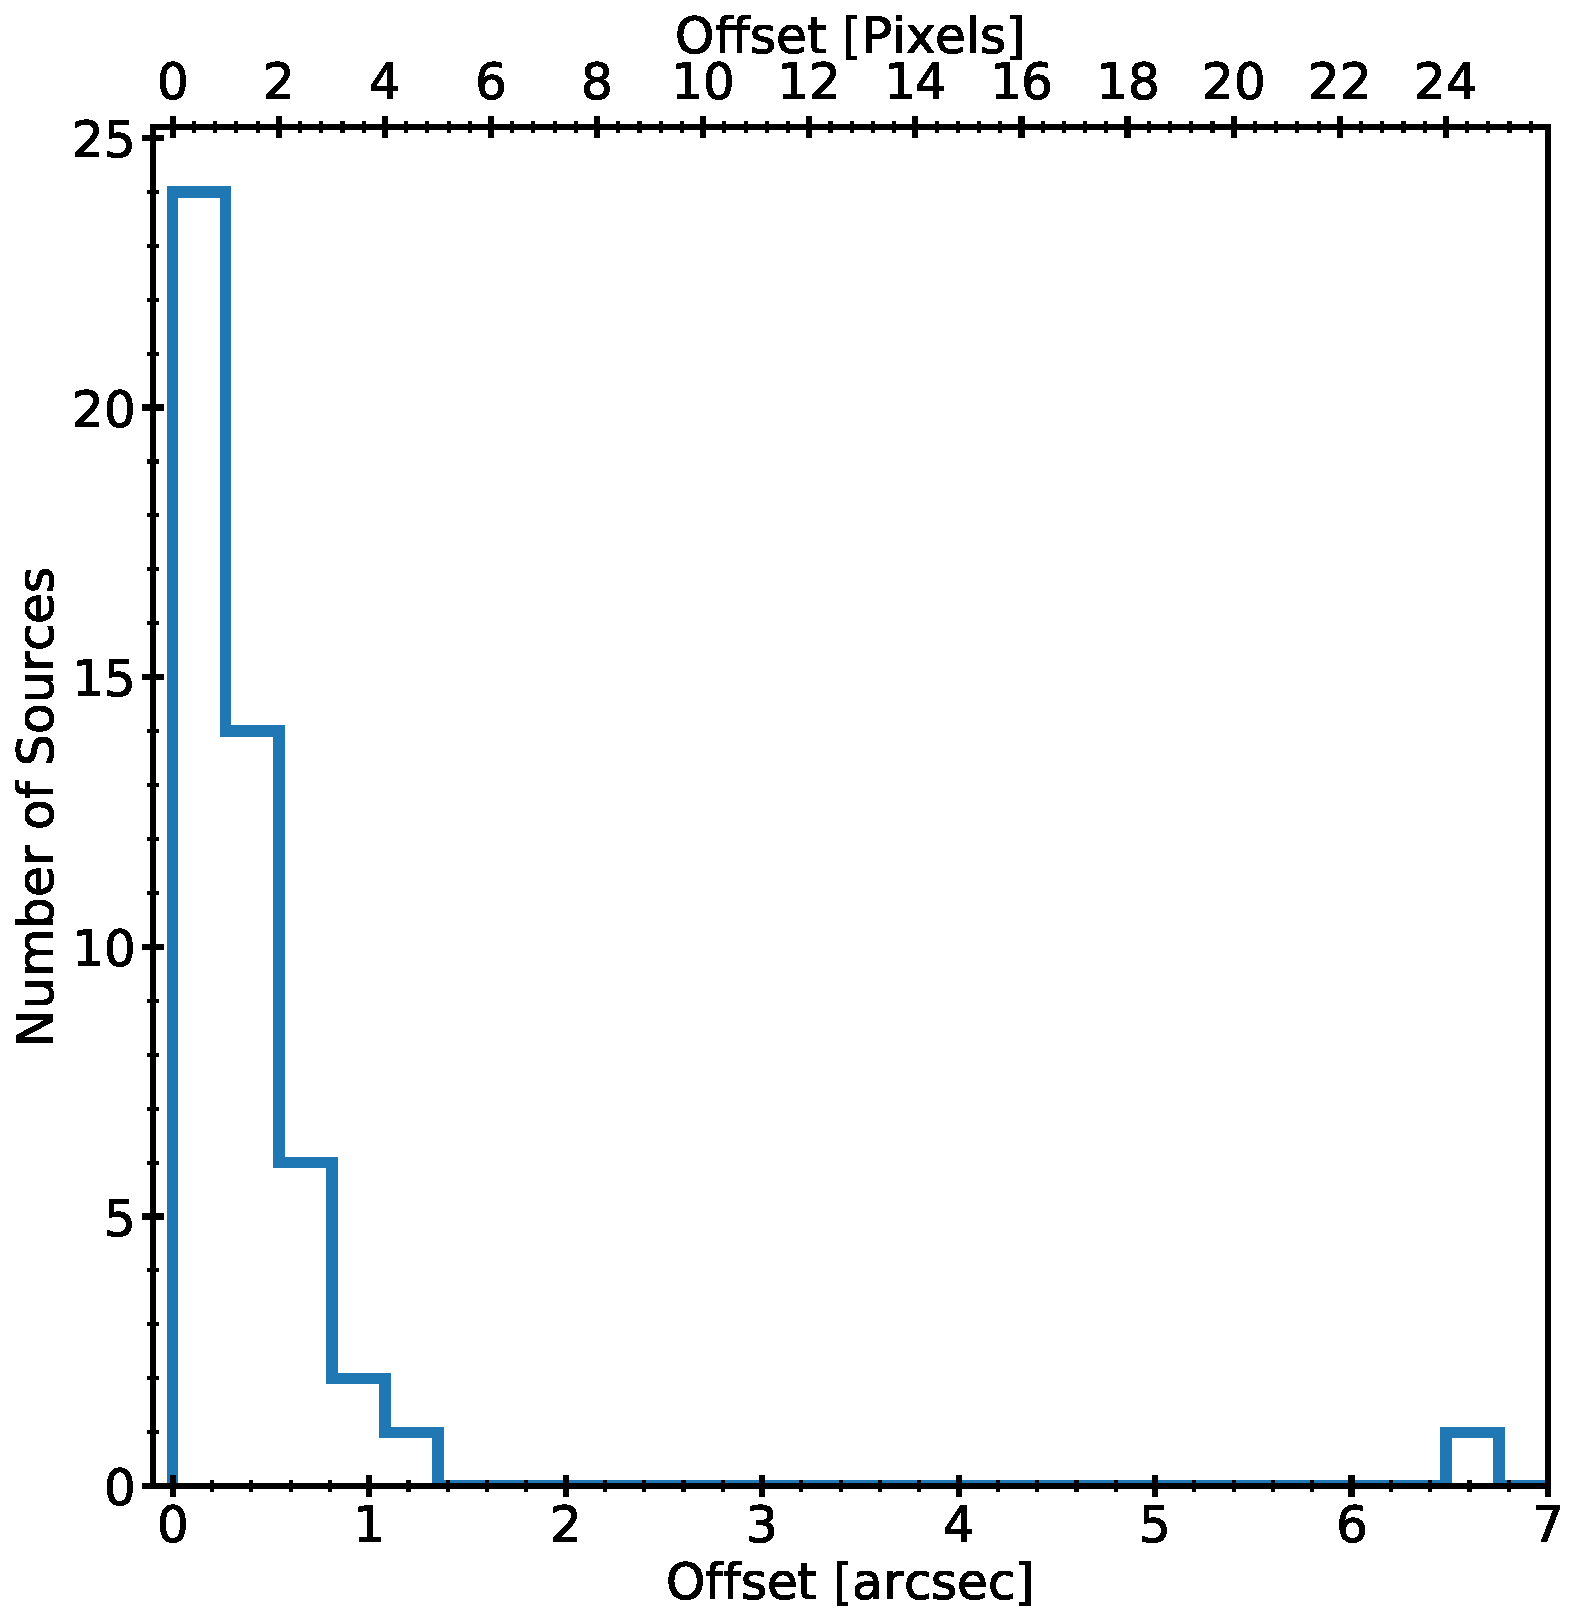
\includegraphics[width=0.9\textwidth]{./figs/chapter3/f1.pdf}}
\caption{\singlespace Offset distribution, with one pixel bins, for sources in Group 2 after visual rejection of image subtraction artifacts. Half (24 of 48) of the sources exhibit offsets smaller than 1 pixel ($0.27\arcsec$), indicating a likely AGN variability origin.}
\label{fig:ch3_offset_hist}
\end{center}
\end{figure}

We note that the single source in \Cref{fig:ch3_offset_hist} with an offset of $\approx6.6\arcsec$, was originally identified with an offset of $0.14\arcsec$. However, manual inspection revealed that the transient had not faded away in the template causing {\tt SExtractor} deblending to detect a low stellarity point source still present on top of the galaxy light distribution. We correct this offset manually, but leave this source in Group 2 as that is the {\it original} classification.

\clearpage
\subsubsection{Groups 3 and 4 -- Point Source Counterparts}
\label{sec:ch3_pointsources}
We are also interested in those candidates that have a coincident point source counterpart in the template images. The presence of such a counterpart disqualifies the source as a kilonova contaminant, but this determination relies on the existence of late-time (or pre-existing) templates.  Therefore, it is still meaningful to construct a census of these sources to gain a better understanding of potential contamination in real-time GW follow-up observations, especially if pre-existing template images are not available. These sources are shown on a color-color diagram in \Cref{fig:ch3_color_color}.

\begin{figure}[!t]
\begin{center}
\hspace*{-0.1in}
\scalebox{1.}
{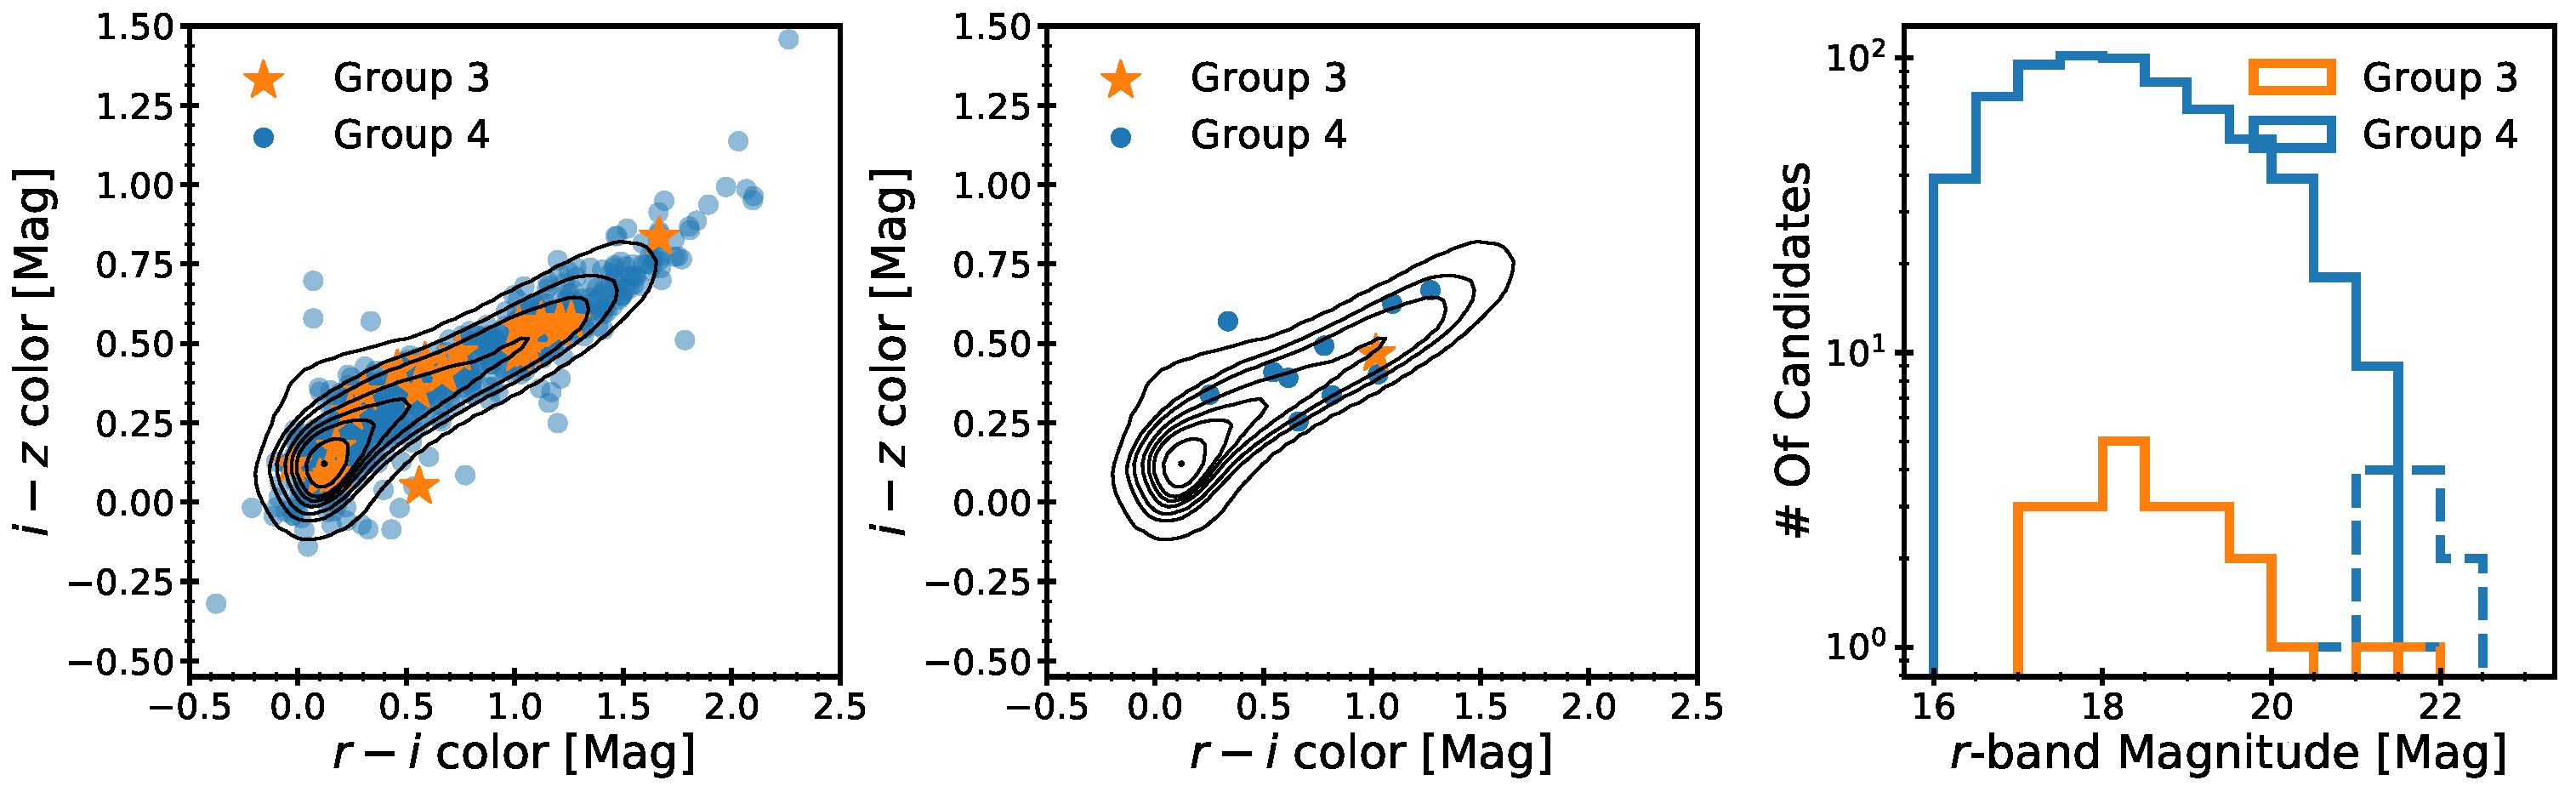
\includegraphics[width=\textwidth]{./figs/chapter3/f2alt.pdf}}
\caption{\singlespace {\it Left:} $r-i$ vs. $i-z$ color-color diagram for the template counterparts identified in Groups 3 (orange stars; \cref{sec:ch3_group3}) and 4 (blue circles; \cref{sec:ch3_group4}). The black contours indicate the stellar locus in our images. We find that the majority of sources are consistent with the stellar locus indicating a variable star origin.
{\it Middle:} Same as top, but only showing those 14 sources that do not have a match in the Gaia DR1 catalog. The majority of sources are still consistent with the stellar locus, indicating that they are stellar but simply too faint to appear in the Gaia catalog.
{\it Bottom:} Distribution of $r$-band magnitudes for sources in Groups 3 and 4. The solid lines indicate sources that have a counterpart in the Gaia DR1 catalog, while dashed lines indicate sources that do not have a catalog match.}
\label{fig:ch3_color_color}
\end{center}
\end{figure}

To help assess if the point source counterpart in the template images is a long-lived transient or simply a stellar variable source, we perform catalog matching for these sources against the Two Micron All-Sky Survey Point Source Catalog (2MASS PSC, \citealt{Skrutskie+06}), the Wide-field Infrared Survey Explorer all-sky release (WISE, \citealt{Wright+10}), and the Gaia DR1 Stellar Catalog \citep{GAIAMainRef,GAIADR1}\footnote{\singlespace We note that Gaia DR1 uses data obtained after our data were obtained. However the time separation between the Gaia mission and our data ($> 1$ yr) along with the comparatively shallow Gaia catalogs (G $\sim$ 20 mag) makes it unlikely that any transient detected in our data will still be present in Gaia DR1.}. This matching is done using the detection coordinates from {\tt photpipe} with a matching radius of $1\arcsec$. This matching identifies 711 of the 725 candidates in Groups 3 and 4. In the following subsections we investigate the two groups separately.

\subsubsection{Group 3 -- Point Source Counterpart With a Bright Nearby Galaxy}
\label{sec:ch3_group3}

We identify 23 sources that are located within $30''$ of a galaxy with $i\lesssim 17.5$ mag. \Cref{fig:ch3_color_color} shows that sources from Group 3 predominantly coincide with the stellar locus indicating a variable star origin, with the galaxy association occurring purely by chance. Given our choice of a chance coincidence probability of $P_{\rm cc} < 0.1$, it is not surprising to find 23 out of 725 spurious matches to galaxies with $i \lesssim 17.5$ mag within $30\arcsec$.

We match these 23 sources against the external catalogs (2MASS, WISE, and Gaia DR1), and find that only one source lacks a catalog match. This source is shown on the color-color diagram in \Cref{fig:ch3_color_color}, and is found to be consistent with the stellar locus. In \Cref{fig:ch3_color_color} we show the distribution of $i$-band magnitudes for Group 3 and we find that the single source not detected in the external catalogs is located at the faint end of our distribution ($r \approx 21.8$~mag). Therefore, this source is simply too faint to appear in the external catalogs.

Based on the presence of a point source counterpart in the template, association with the stellar locus, and matches to external catalogs, we conclude that none of the 23 sources in Group 3 can be considered as kilonova contaminants provided that deep template images are available. If templates are not available, then the single source without a counterpart in the Gaia DR1 catalog would be considered a kilonova contaminant.

\subsubsection{Group 4 -- Point Source Counterpart Without a Bright Nearby Galaxy}
\label{sec:ch3_group4}

The remaining 702 sources do not have an associated galaxy that meets our matching criteria. We show these sources in the color-color diagram (\Cref{fig:ch3_color_color}). Similar to the candidates in Group 3, these sources coincide almost entirely with the stellar locus. The sources that extend to redder colors ($i-z \gtrsim 0.75$ mag and $r-i \gtrsim 1.75$ mag) are also consistent with the stellar locus; the contours simply do not capture this sparser region of the locus. We manually inspect sources that appear to lie outside of the stellar locus. We find that half of these sources have one or more masked/saturated pixels that bias their photometry. The remaining sources are blended or positioned in the halo of a saturated star, which affects their photometry. Finally, there is a single source with no obvious photometric issues. As we show below, this source is not detected in any external catalog, but this is likely due to its faintness ($r \approx 21.7$ mag and $g \gtrsim 23.0$ mag). Furthermore, this source does not appear near an obvious host galaxy. It is therefore most likely a faint variable star or quasar.

Matching the sources in Group 4 against the external catalogs, we find that all but 13 of these sources have a match in 2MASS, WISE, or Gaia DR1. We show 10 of these 13 unmatched sources on the color-color diagram in \Cref{fig:ch3_color_color} showing that they are consistent with the stellar locus.\footnote{\singlespace The remaining 3 sources are not plotted due to a lack of $r$- or $z$-band detections.} Inspecting the magnitude distribution in \Cref{fig:ch3_color_color}, we find that these sources are located at the faint end of our distribution. All of the sources exhibit $r > 20.5$ mag, indicating that they are too faint to be present in the Gaia DR1 catalog. As with Group 3, we conclude that none of these sources can be considered kilonova contaminants, {\it as long as} sufficiently deep template images are available.

\subsubsection{Summary of Initial Search}
\label{sec:ch3_search_summary}
We find 48 sources that can be considered as potential kilonova contaminants. All of these sources are from Group 2, appearing in coincidence with galaxies, and with half (24 sources) having a separation of $\lesssim 1$ pixel from the galaxy nucleus, suggesting that they are likely due to AGN variability. While it is possible for kilonovae to appear in the nuclear regions of their hosts, we generally expect larger offsets based on the fact that only $\approx 15\%$ of SGRBs exhibit offsets of $\lesssim 0.5 R_{1/2}$ \citep{FongBerger13,Fong+13,Berger2014}. In this analysis we do not eliminate nuclear sources from consideration, but we note that in an actual follow-up search such sources could in principle be deprioritized.

We note that rejection of the 14 sources with point-source counterparts possessing stellar colors in the template images but lacking a catalog match in Groups 3 and 4 as potential kilonova candidates is made under the assumption of template images being available. However, in the context of real-time detection in the absence of pre-existing templates such sources may lead to an additional source of contamination. We do not include these sources in our contaminant sample, because they can ultimately be rejected, but we caution that the rate of contaminants may be up to $\approx 25\%$ higher if such sources cannot be efficiently rejected.

\subsection{Color Selection of Kilonova Contaminants}
\label{sec:ch3_kn_search}
We now study the $i-z$ colors of the 48 potential contaminants to identify sources that can mimic either red or blue kilonova emission. The color distribution for all 48 sources is shown in \Cref{fig:ch3_color_dist_final}. The $i-z$ color is computed as a signal-to-noise-weighted average using the ``forced" {\tt DoPhot} photometry from the difference images. We define red kilonova contaminants as those having $i-z \gtrsim 0.5$~mag \citep{BarnesKasen13,CowpBerger15}. For blue kilonova contaminants we require $i-z \lesssim 0.0$~mag, motivated by the models of \cite{Kasen+15} for a BNS merger that results in a HMNS with $t_{\rm HMNS}\gtrsim 100$ ms. These criteria are shown in \Cref{fig:ch3_color_dist_final}. These criteria capture the tails of the color distribution, with over half of the sources (27 of 48) exhibiting $i-z = 0.0-0.5$~mag.

\begin{figure}[!t]
\begin{center}
\hspace*{-0.1in}
\scalebox{1.}
{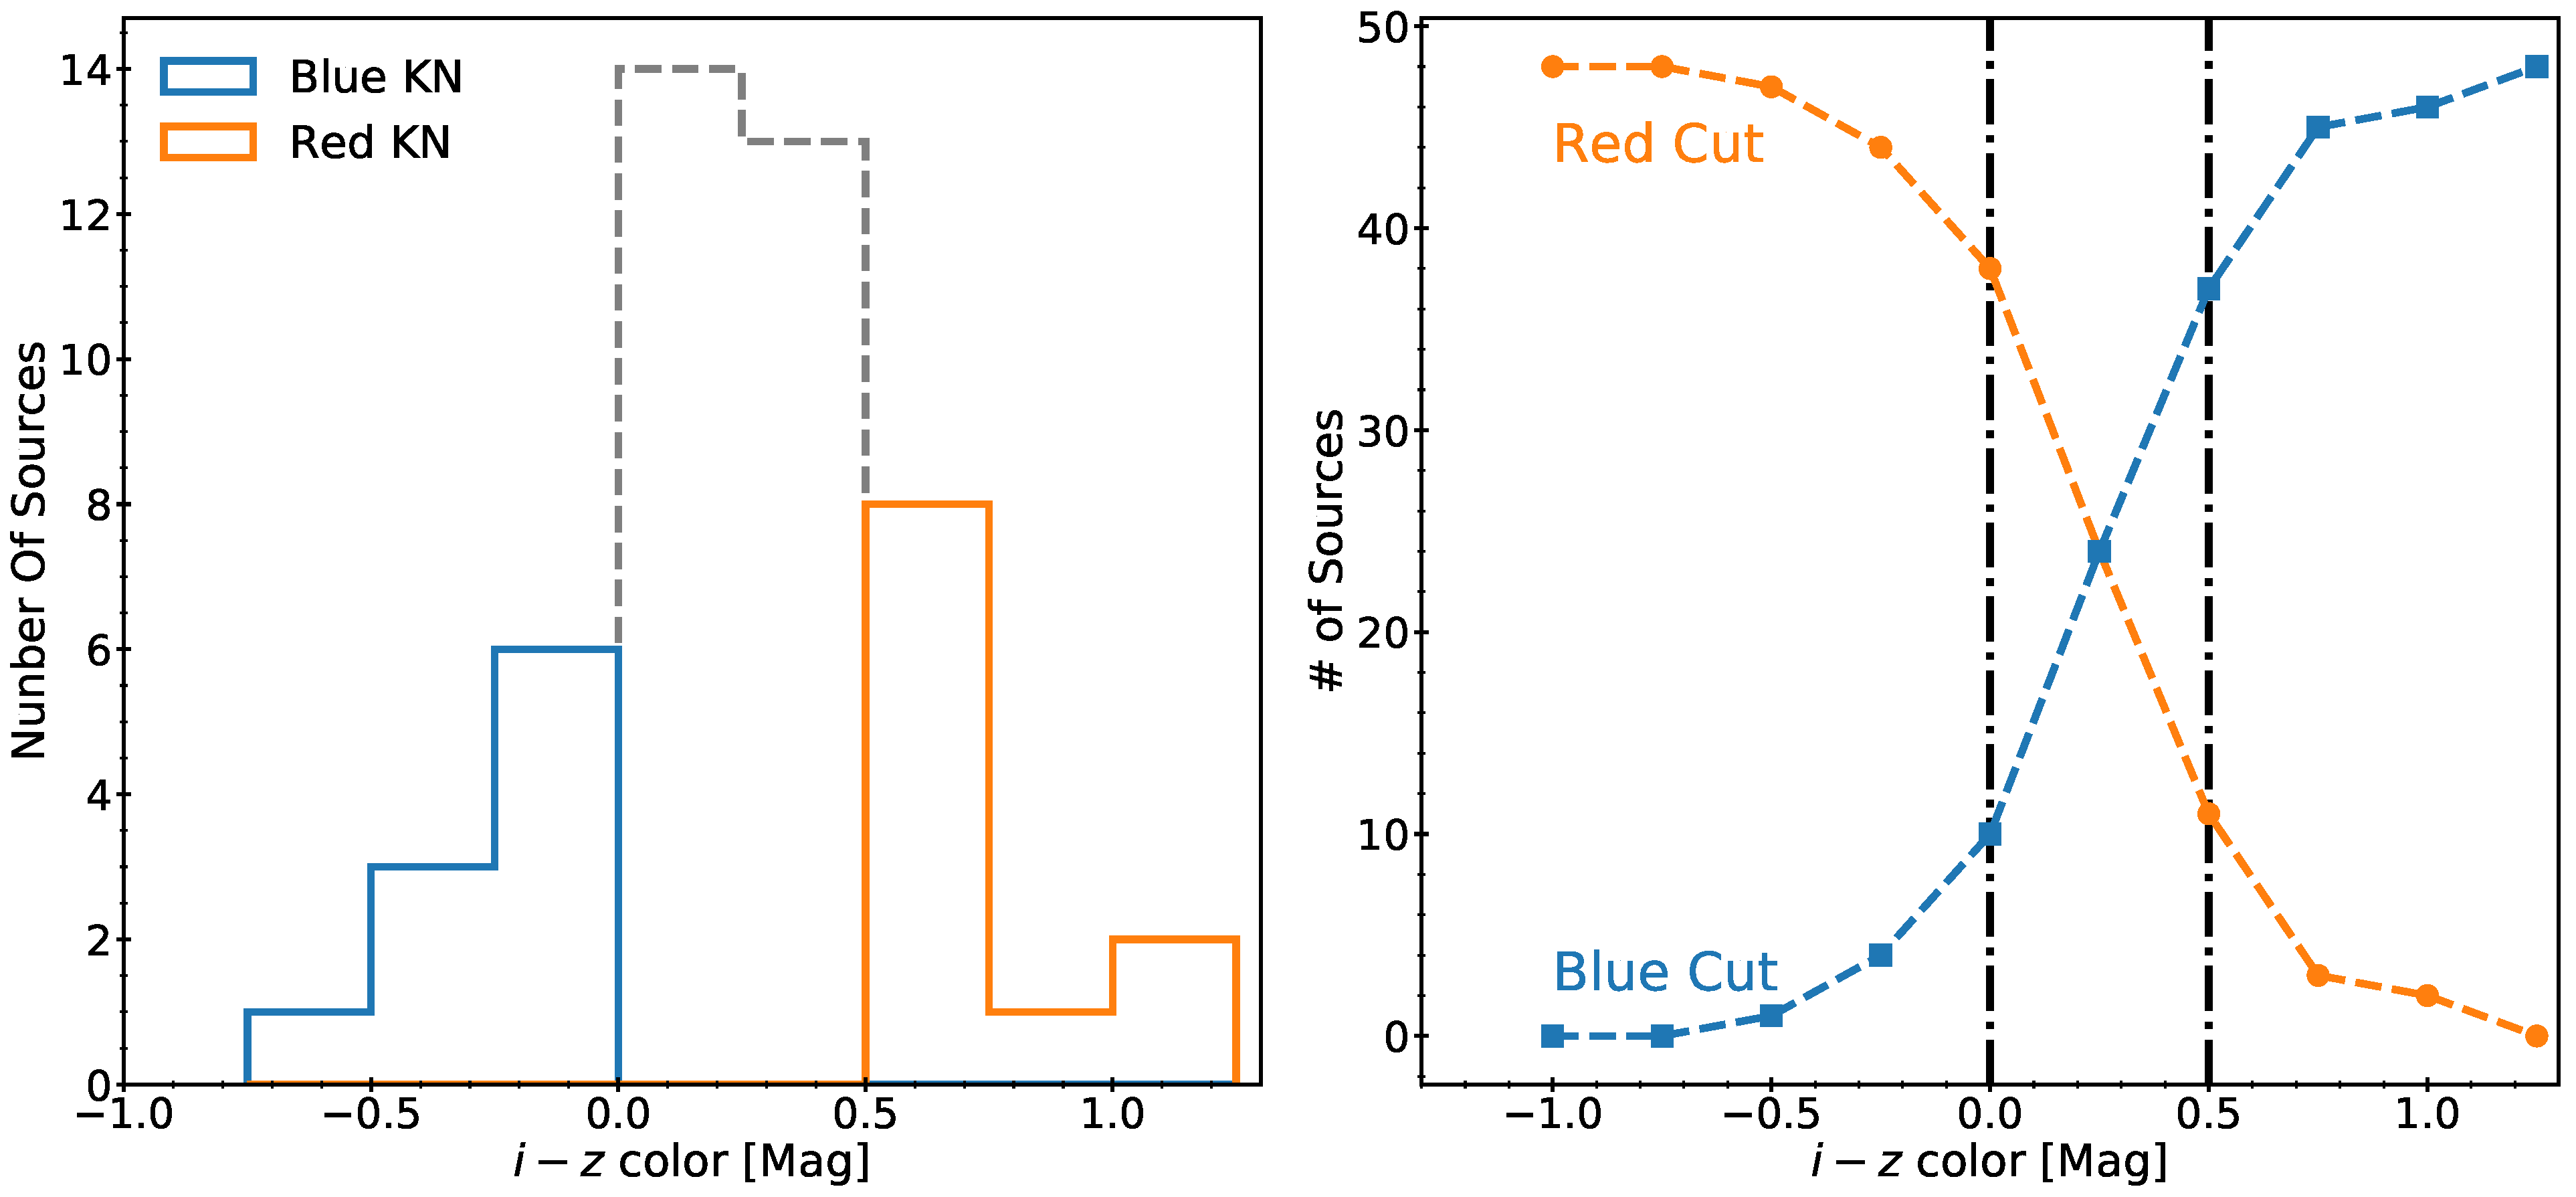
\includegraphics[width=\textwidth]{./figs/chapter3/f3.pdf}}
\caption{\singlespace {\it Left:} $i-z$ color distribution for the 48 sources considered in this analysis. The 11 sources identified as red kilonova contaminants are plotted in orange (\cref{sec:ch3_kn_search}), while the 10 sources identified as blue kilonova contaminants are shown in blue (\cref{sec:ch3_kn_search}). The remaining 27 sources from Group 2 are plotted in grey dashed lines.
{\it Right:} The number of sources recovered by performing an $i-z$ color cut on the sample of 48 sources in Group 2. The orange line gives the number of sources redder than a given $i-z$ color. The blue line indicates the number of sources bluer than a given color cut. The vertical black lines indicate our nominal cuts of $i-z < 0$~mag and $i-z > 0.5$~mag, for blue and red kilonovae, respectively. The sharp increase in the number of sources as the chosen color threshold is relaxed can be clearly seen.}
\label{fig:ch3_color_dist_final}
\end{center}
\end{figure}

We find 11 sources that satisfy the color criterion for a red kilonova, of which 6 ($54\%$) are located within a pixel of a galaxy nucleus.  The light curves of all 11 sources are shown in \Cref{fig:ch3_final_lc_red}. The majority of these sources (8 of 11) have $i-z \approx 0.5-0.8$~mag and only two sources (\#75 and \#2948) have $i-z \gtrsim 1$~mag. Key aspects of the temporal evolution of red kilonova models are the rapid rise to peak ($\sim \rm few$ days) and the rapid decline post-peak ($\delta m_i \gtrsim 0.3$~mag~day$^{-1}$), in both $i$- and $z$-bands. Manually inspecting the light curves in \Cref{fig:ch3_final_lc_red}, we find no sources that clearly satisfy either of these criteria.

\begin{figure}[!t]
\begin{center}
\hspace*{-0.1in}
\scalebox{1.}
{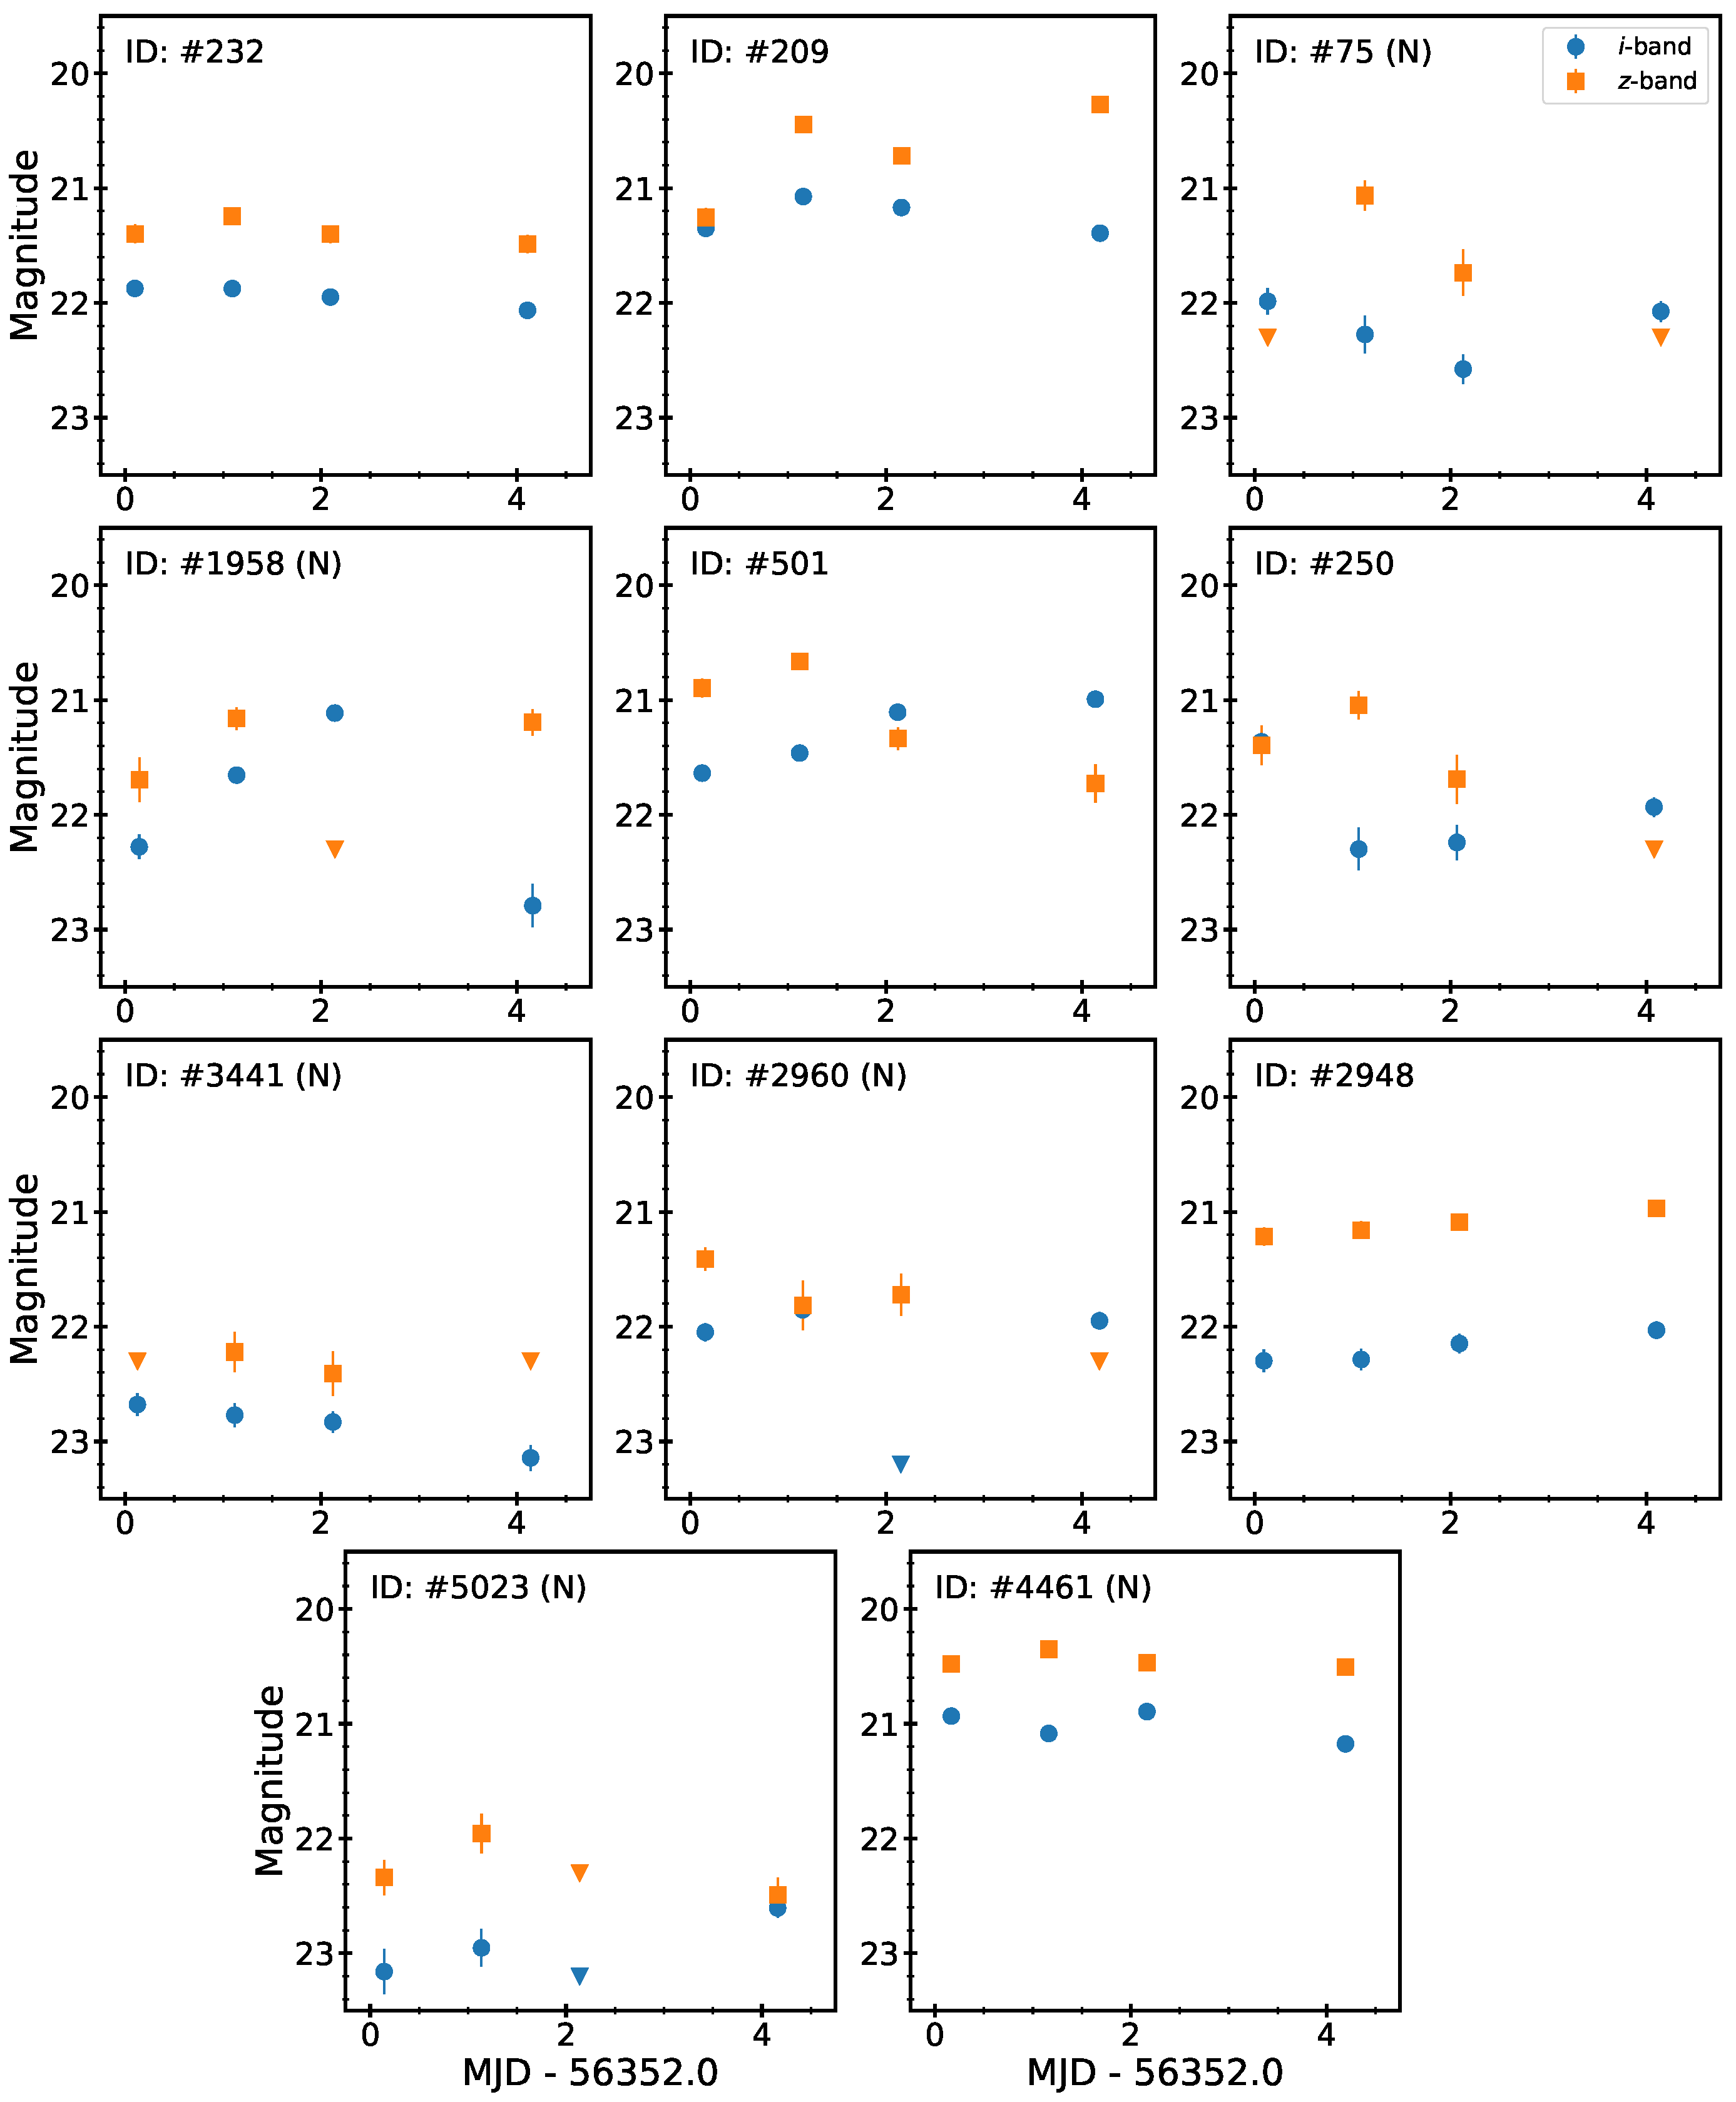
\includegraphics[width=0.825\textwidth]{./figs/chapter3/f4.pdf}}
\caption{\singlespace Light curves for the 11 sources in our red kilonova contaminant sample, constructed from the ``forced" {\tt DoPhot} PSF photometry (blue circles: $i$-band; orange squares: $z$-band). Nuclear sources are indicated by an (N) in the ID number. The $5\sigma$ limits for non-detections are indicated by triangles.}
\label{fig:ch3_final_lc_red}
\end{center}
\vspace{0.5cm}
\end{figure}

\begin{figure}[!t]
\begin{center}
\hspace*{-0.1in}
\scalebox{1.}
{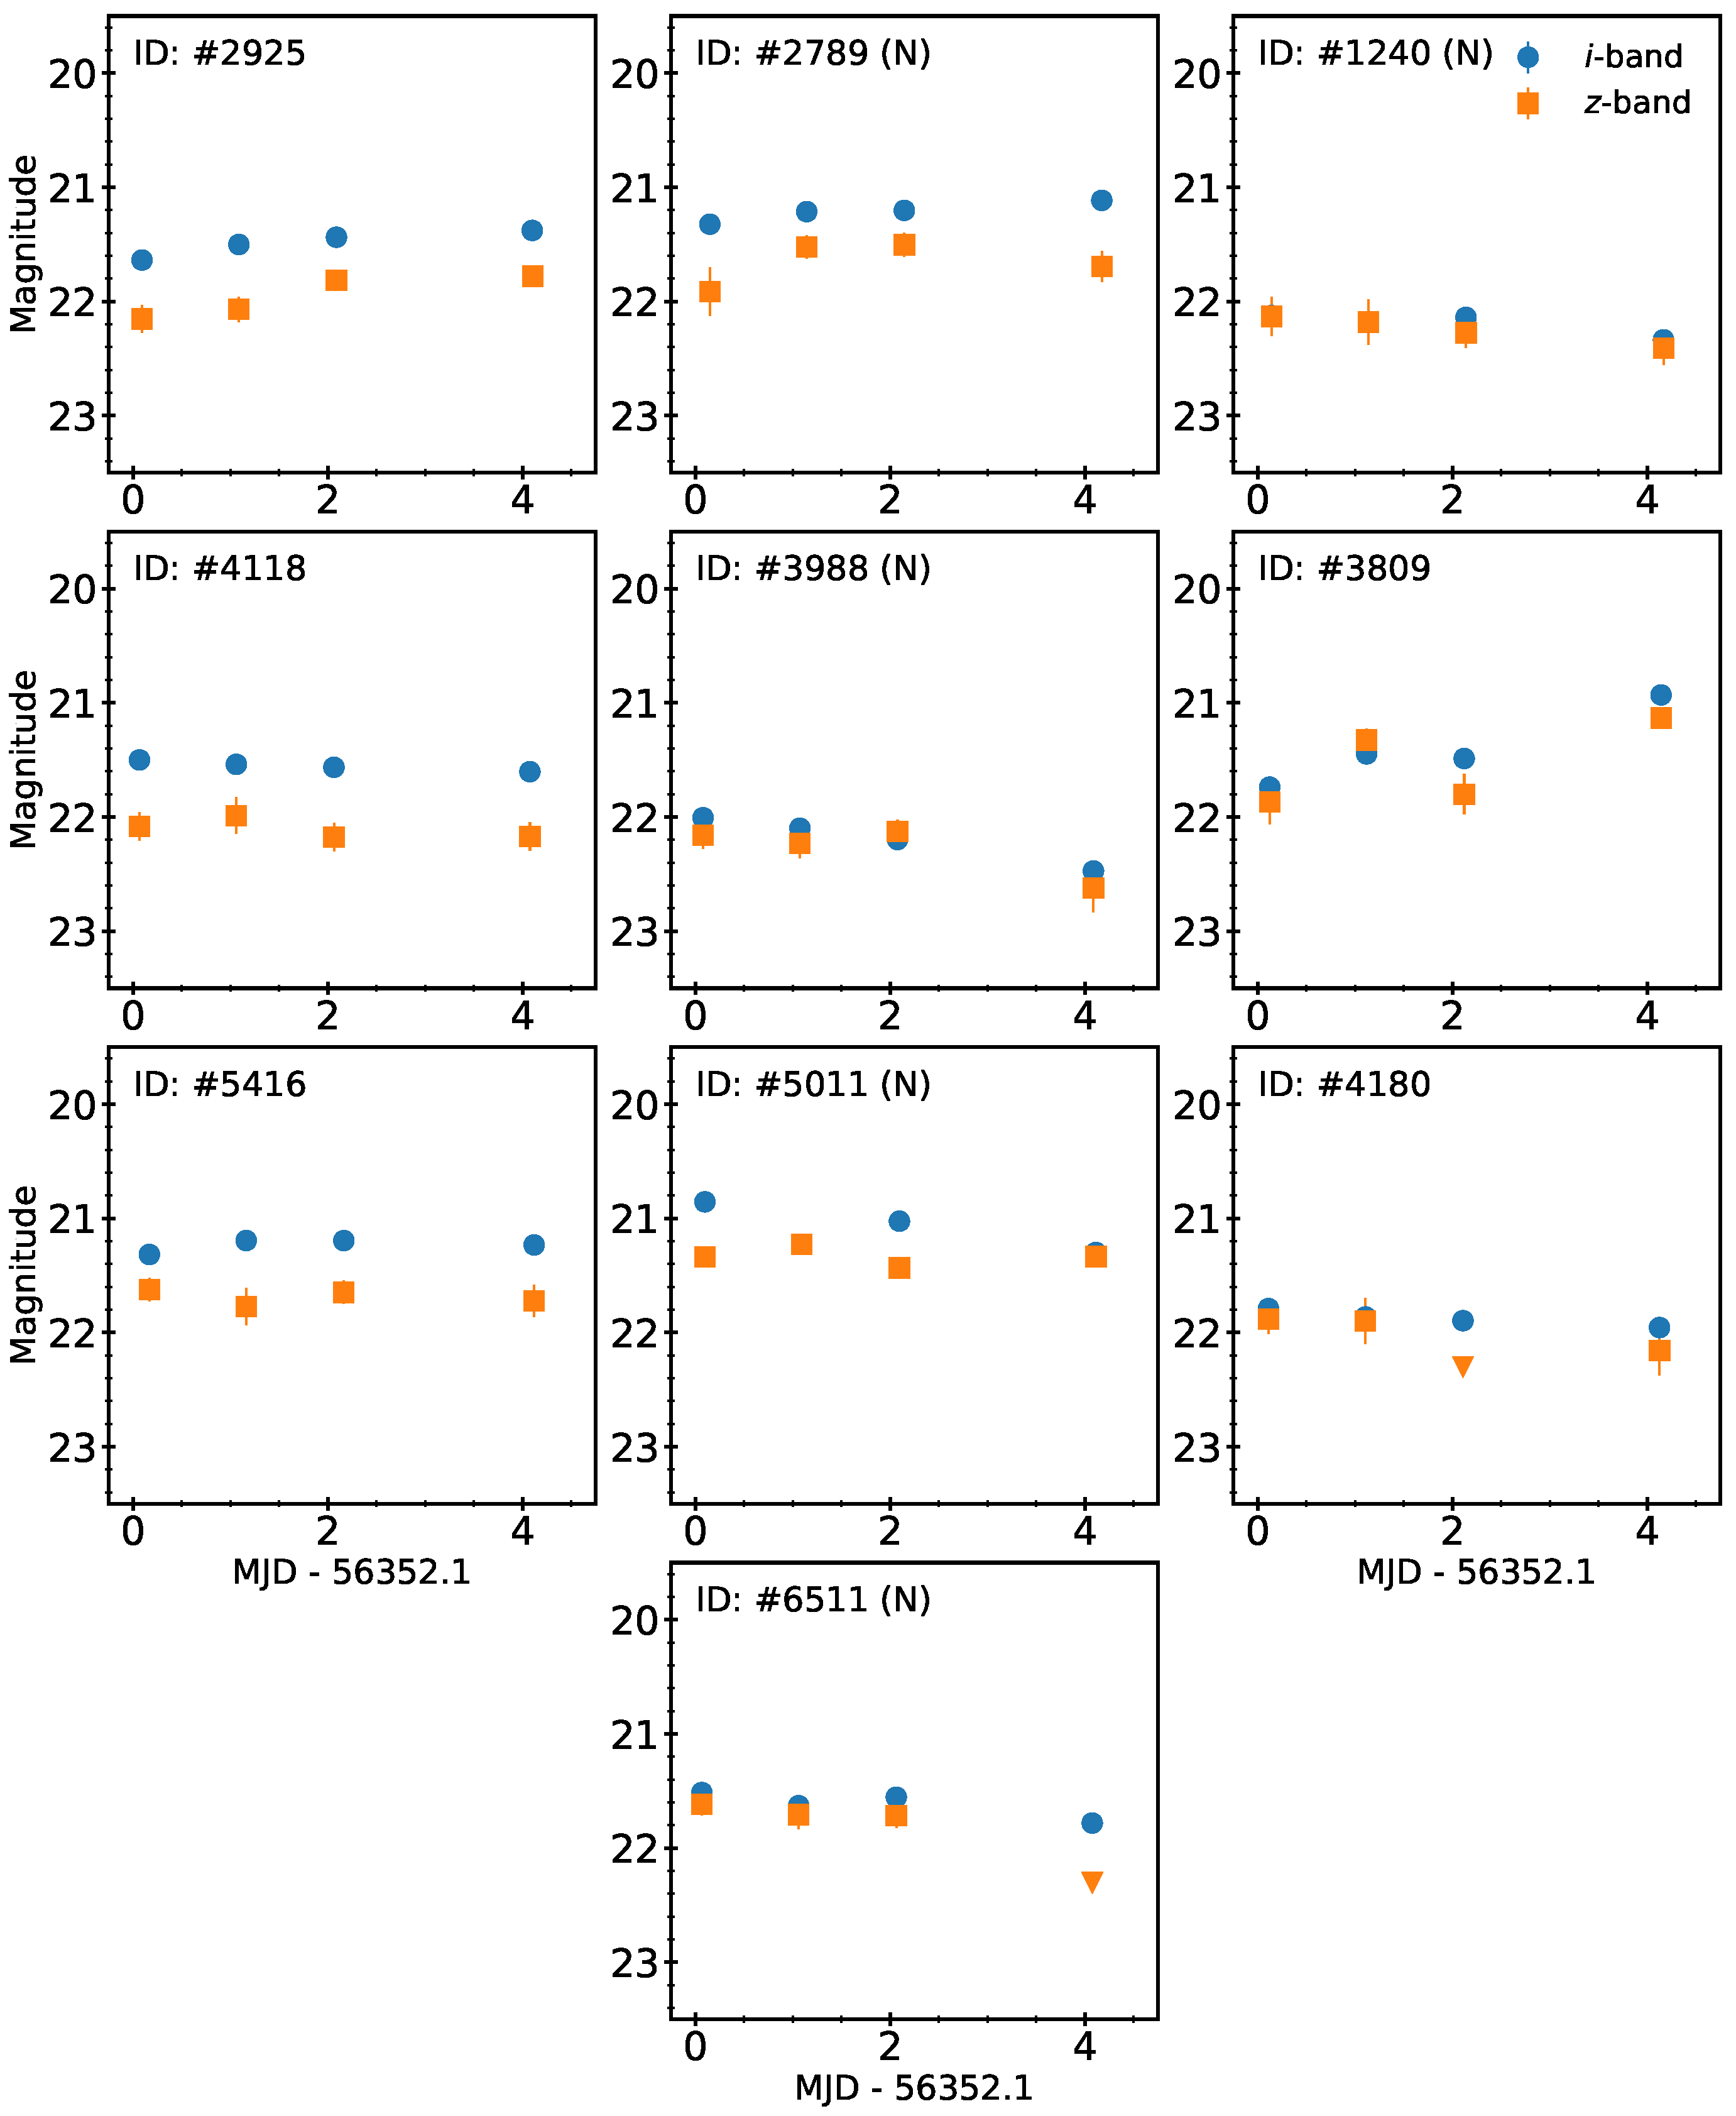
\includegraphics[width=0.9\textwidth]{./figs/chapter3/f5.pdf}}
\caption{\singlespace Same as \Cref{fig:ch3_final_lc_red}, but for the sources in the blue kilonova contaminant sample.}
\label{fig:ch3_final_lc_blue}
\end{center}
\vspace{1.1cm}
\end{figure}

\clearpage
We find 10 sources that have colors expected for blue kilonovae. About half of these sources are located within a pixel of a galaxy nucleus. We show the light curves of all 10 sources in \Cref{fig:ch3_final_lc_blue}. The temporal evolution of blue kilonova models is more rapid, with a shorter duration, than that of red kilonovae. We do not find any systematic trends in light curve behavior for the 10 sources, or when inspecting the nuclear and non-nuclear sources separately.

The complete set of selections are summarized in \cref{tab:ch3_cuts_sum}. We selected subsets of red and blue kilonova contaminants with specific color cuts, but we note that the models motivating these choices have uncertainties that can affect the kilonova colors (e.g., ejecta mass and velocity, ejecta composition, uncertainties in $r$-process opacities, etc.). This makes understanding the effect of color criteria on the size of the contaminant sample crucial.

\singlespace
\begin{deluxetable}{l c c c c}
\tabletypesize{\footnotesize}
\tablecolumns{5}
\tablewidth{0pt}
\tablecaption{Summary of Final Contaminant Sample at $i\lesssim 22.5$ mag
\label{tab:ch3_cuts_sum}}
\tablehead{
	\colhead{Selection} &
	\colhead{$N$ (Raw)} &
	\colhead{$\mathcal{R}$ (Raw)} &
	\colhead{$N$ (Corrected)} &
	\colhead{$\mathcal{R}$ (Corrected)} \\
	\colhead{} &
	\colhead{} &
	\colhead{(deg$^{-2}$)} &
	\colhead{} &
	\colhead{(deg$^{-2}$)}
}
\startdata
Total Sample & 45$_{-9}^{+10}$ & 0.80$_{-0.16}^{+0.18}$ & 101$_{-14}^{+15}$ & 1.79$_{-0.25}^{+0.26}$ \\
Nuclear & 21$_{-6}^{+ 7}$ & 0.38$_{-0.11}^{+0.12}$ & 58$_{-10}^{+12}$ & 1.03$_{-0.19}^{+0.20}$ \\
Non-Nuclear & 24$_{-7}^{+ 7}$ & 0.43$_{-0.12}^{+0.13}$ & 43$_{-8}^{+10}$ & 0.76$_{-0.15}^{+0.17}$ \\
Red & 9$_{-4}^{+ 4}$ & 0.16$_{-0.07}^{+0.07}$ & 12$_{-4}^{+ 5}$ & 0.20$_{-0.07}^{+0.09}$ \\
Blue & 10$_{-4}^{+ 5}$ & 0.18$_{-0.07}^{+0.09}$ & 46$_{-8}^{+11}$ & 0.82$_{-0.16}^{+0.18}$ \\
Red/Nuclear &  4$_{-3}^{+ 3}$ & 0.07$_{-0.05}^{+0.05}$ &  5$_{-2}^{+ 4}$ & 0.09$_{-0.05}^{+0.05}$ \\
Blue/Nuclear &  5$_{-3}^{+ 3}$ & 0.09$_{-0.05}^{+0.05}$ & 34$_{-7}^{+ 9}$ & 0.60$_{-0.14}^{+0.15}$ \\
Red/Non-Nuclear &  5$_{-3}^{+ 3}$ & 0.09$_{-0.05}^{+0.05}$ &  7$_{-3}^{+ 4}$ & 0.11$_{-0.06}^{+0.07}$ \\
Blue/Non-Nuclear &  5$_{-3}^{+ 3}$ & 0.09$_{-0.05}^{+0.05}$ & 13$_{-4}^{+ 5}$ & 0.22$_{-0.08}^{+0.08}$ \\
Timescale: $3-24$ hr & $\lesssim 3$ & $\lesssim 0.05$ & $\lesssim 4$ & $\lesssim 0.07$ \\
Timescale: $\lesssim3$ hr & $\lesssim 3$ & $\lesssim 0.05$ & $\lesssim 4$ & $\lesssim 0.07$ \\
\enddata
\tablecomments{Summary of selections made for our magnitude-limited final sample of 45 sources, including $1 \sigma$ errors on source counts. We give raw and efficiency corrected number of sources $(N)$ and sky rate $(\mathcal{R})$, assuming our search represents a typical region of sky. We define red and blue sources as those with $i-z > 0.5$~mag and $i-z < 0.0$~mag, respectively. We define nuclear sources as those exhibiting an offset from the nucleus of their host galaxy of $\lesssim 1$ pixel ($\lesssim 0.27\arcsec$).}
\end{deluxetable}
\doublespace

The number of red and blue kilonova contaminants as a function of color is shown in \Cref{fig:ch3_color_dist_final}. We find that the number of sources in either sample increases significantly if the selection on $i-z$ color is relaxed. For example, if we search for red kilonova contaminants by requiring $i-z \gtrsim 0.3$~mag, the number of contaminants rises to 22, a twofold increase. Similarly, if we relax our color selection for blue kilonova to $i-z \lesssim 0.2$~mag, the number of contaminants rises to 20, again a twofold increase over the original sample.

\clearpage
\subsection{A Search for Contamination on Nightly Timescales}
\label{sec:ch3_kn_short}
We also search our data for sources that could appear as contaminants on the timescales relevant to the short-lived ``neutron precursor," that are speculated to accompany some mergers (\cref{sec:ch3_kn_models}, \citealt{Metzger+15}). We accomplish this by leveraging the rapid cadence of our observations to identify potential contaminants that are detected during a single night, or just a half-night epoch, probing transient and variable events that occur with timescales of $3$ hr to 1 day and $\lesssim3$ hours, respectively. We search for candidates based on their behavior in the ``forced" {\tt DoPhot} photometry as follows:

\begin{enumerate}
\item We search for transients with a characteristic timescale of 3 hours to 1 day by selecting candidates that exhibit two $\gtrsim 10\sigma$ detections in $i$-band during a single night of observations (i.e., two epochs). Outside of these epochs, the sources must exhibit an $i$-band difference flux that is a factor of $\gtrsim 10$ fainter than the maximum $i$-band difference flux measured during the night of interest. This requirement is consistent with the rapid fading expected for ``neutron precursors" \citep{Metzger+15}.

\item We search for transients with characteristic timescales of $\lesssim 3$ hours by selecting candidates that exhibit a single $\gtrsim 10\sigma$ detection in both $i$- and $z$-band in a single epoch. Outside of this epoch, the sources must exhibit a difference flux that is a factor of $\gtrsim 10$ fainter than the difference flux measured during the epoch of interest, in both $i$- and $z$-bands, again motivated by the rapid fading expected for ``neutron precursors" \citep{Metzger+15}.
\end{enumerate}

\clearpage
We find 9 sources with a timescale between 3 hours and 1 day. We perform a manual inspection of this sample, finding 5 genuine sources and 4 that result from image subtraction artifacts. Matching the 5 sources to our template images and external catalogs, we find that all of them have a point-source match in both our template images and Gaia DR1, and hence represent stellar variability or flaring. We find no evidence for extragalactic contamination from sources with a timescale between 3 hours and 1 day.

We find 39 sources that match our selection criteria for a duration of $\lesssim 3$ hr. We manually inspect these sources and find 24 genuine sources, with the remaining candidates resulting from image subtraction artifacts. Fifteen of these sources have point source counterparts in our template images, as well as matches in the Gaia DR1 catalog. An additional six sources are matched to high stellarity sources, but these are all likely too faint ($r \gtrsim 21.5$~mag and $g \gtrsim 23.0$~mag) to be present in the Gaia DR1 catalog. The remaining 3 sources exhibit significant trailing in at least one epoch and no detected counterpart in the template images, indicating that they are asteroids. Thus, we find no non-stellar or non-moving sources with a timescale of $\lesssim 3$ hr.

\section{Detection Efficiency}
\label{sec:ch3_fakes}
To determine the areal rate of the various kilonova contaminants we need to determine the detection efficiency of our search method. We accomplish this by injecting point sources into both our search and template images. We inject each source with a constant brightness and $i-z$ color in the search images. To assess the impact of residual flux in the template images we use a range of fading levels between the search and template images.  Finally, to assess the effect of host galaxy brightness on our recovery efficiency we inject the sources on and near galaxies identified using {\tt SExtractor} photometry on the template epoch.

We inject ten point sources around 580 galaxies identified across the 21 fields in our dataset for a total of 5800 injected sources. The population is constructed as follows:

\begin{enumerate}
\item We select extended sources by requiring a half-light radius of $R_{1/2} > 20$ pixels and a stellarity value of $<0.2$. The choice of $R_{1/2}$ corresponds to the approximate size of a Milky Way like galaxy at a distance of $\approx 200$ Mpc, appropriate for NS-NS mergers detections by aLIGO. These values are determined from the {\tt FLUX\_RADIUS} and {\tt CLASS\_STAR} parameters in the {\tt SExtractor} catalog \citep{BertinArnouts96}, and verified by manual inspection.

\item We inject 10 sources at random locations around each galaxy, constrained to a box that is $4R_{1/2}$ on a side.

\item We inject sources with an $i$-band magnitude range of $19.5-23$ mag, with a volume weighting to produce a realistic distribution of faint sources.

\item We assign each source a color of $i-z=-1$ to $1$ mag, with a uniform distribution.

\item We assign each source a difference in magnitude between the science and template images of $\delta m= 0.2-3$ mag, with a uniform distribution; the range is designed to capture slow fading that would be typical of supernovae and rapid fading typical of kilonovae.

\end{enumerate}

\clearpage
To recover and study the injected sources we process the data in the same manner as described in \cref{sec:ch3_obs}, and apply the data quality selection criteria as described in \cref{sec:ch3_data_cuts}. We then match the identified sources against the list of injected sources, allowing for an astrometric match tolerance of 2 pixels.

For the purpose of determining our detection efficiency in a manner relevant to our search for kilonova contaminants we identify two primary groups of injected sources, namely those that have red kilonova properties (i.e., $i-z>=0.5$ mag and $\delta_m>=1$ mag) and those that have blue kilonova properties (i.e., $i-z<=0.0$ mag and $\delta_m>=1$ mag). These criteria lead to 1006 and 1955 injected sources, respectively. The remaining 2839 sources span a range of properties between red and blue kilonovae. We consider the effect of the source brightness, color, fading, and the separation from the host galaxy on our ability to detect sources. We define our efficiency as the ratio of the number of sources recovered to the number of sources injected.

In \Cref{fig:ch3_eff_1D} we plot the detection efficiency as a function of $i$-band magnitude for the full sample, as well as for the subsets of red and blue kilonova sources. We find an overall efficiency of $\gtrsim0.8$ for $i \lesssim 21.5$ mag and 0.5 at $i \approx 22$ mag. For red kilonova sources we find a higher efficiency of $\approx 0.9$ at $i\lesssim 22$ mag, and 0.5 at $i\approx 22.8$ mag. Our efficiency for blue kilonova sources is $\approx 0.9$ for sources with $i\lesssim 21$ mag, and 0.5 at $i\approx 21.5$ mag. The higher efficiency for red kilonova sources is due to the relative depths of our $i$- and $z$-band images, which were chosen to explore red sources.

\begin{figure}[!t]
\begin{center}
\hspace*{-0.1in}
\scalebox{1.}
{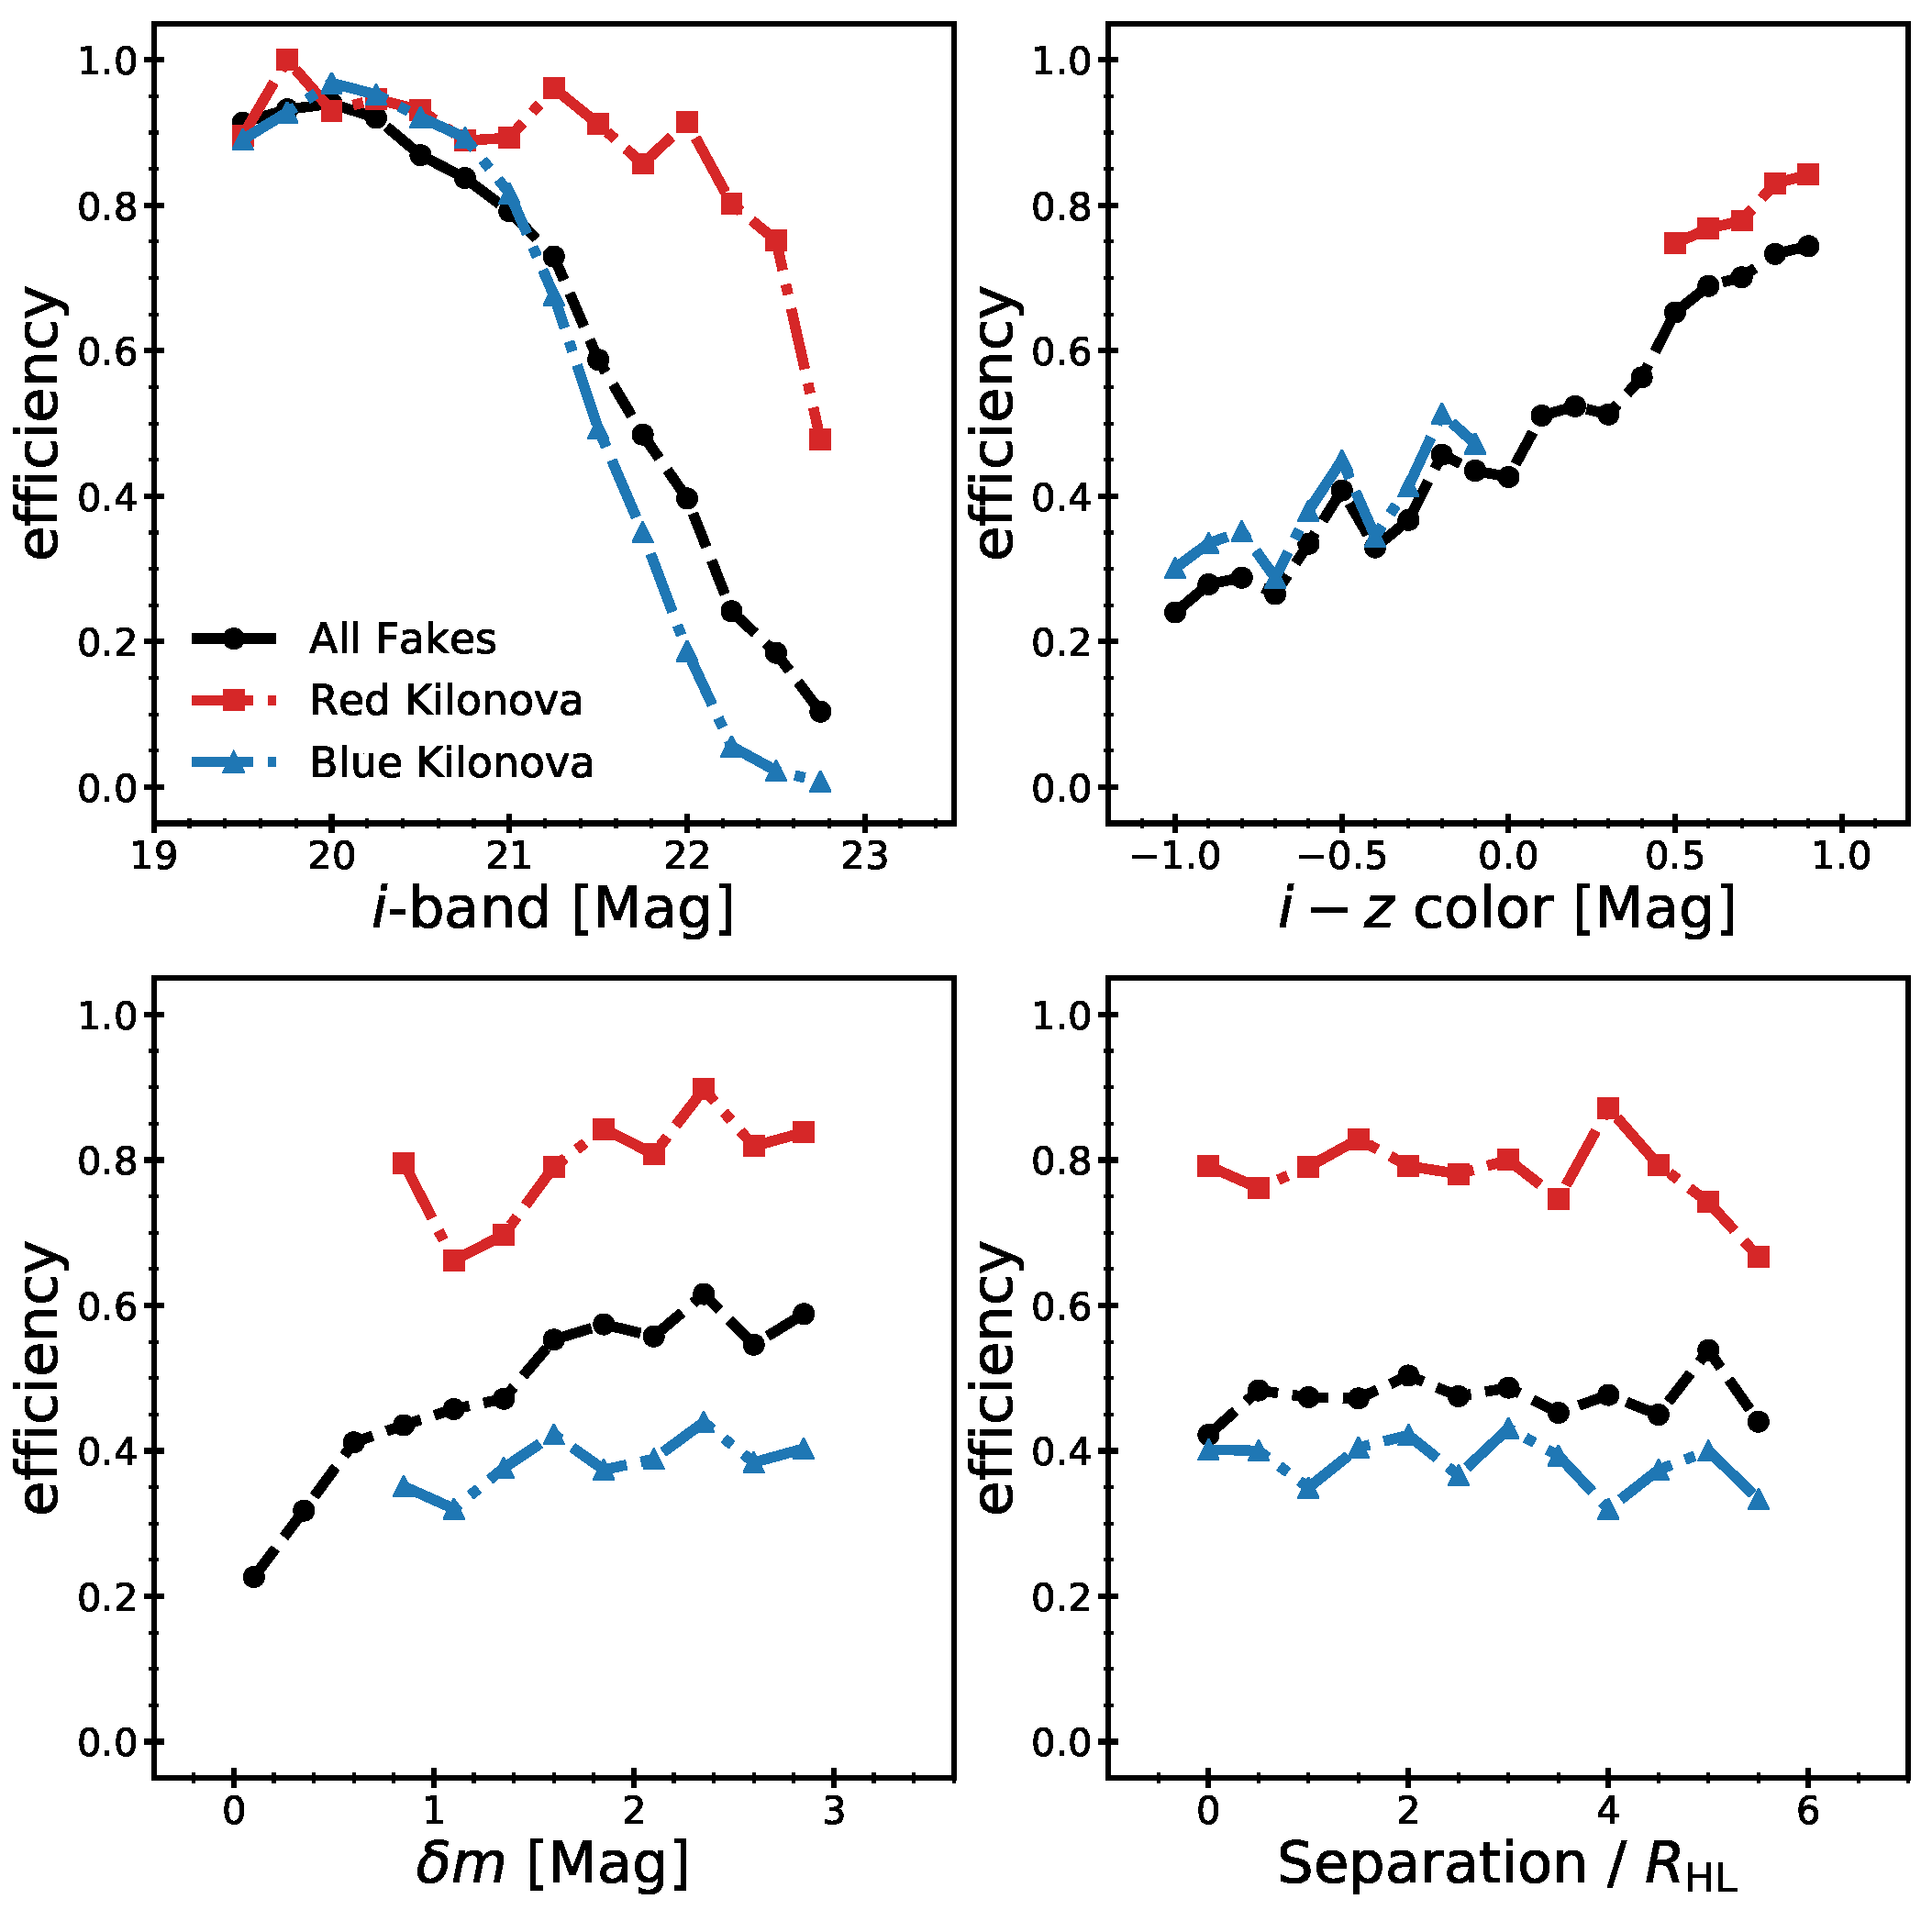
\includegraphics[width=0.85\textwidth]{./figs/chapter3/f6.pdf}}
\caption{\singlespace \singlespace Plots of recovery efficiency as a function of various fake source injection parameters. The efficiency for the entire population of fake sources is shown as a black line while the efficiency for red kilonova and blue kilonova fake sources are shown as orange and blue lines, respectively. {\it Top Left:} Efficiency as a function of $i$-band magnitude. We note that our efficiency for red kilonova fake sources is higher than our mean efficiency, while the blue kilonova efficiency declines more rapidly compared to the red kilonova fake sources. This is due to the design of our observations, which are aimed at red sources. {\it Top Right:} Efficiency as a function of $i-z$ color. We are more sensitive to objects that are red in $i-z$ color, which drives the efficiency differences seen in the other panels. {\it Bottom Left:} Efficiency as a function of fading ($\delta m$, see text for definition). {\it Bottom Right:} Efficiency as a function of host galaxy separation. We find no dependence on separation.}
\label{fig:ch3_eff_1D}
\end{center}
\end{figure}

The efficiency as a function of color for all magnitudes and fading rates is also shown in \Cref{fig:ch3_eff_1D}. We find that the efficiency is $\lesssim 0.5$ for $i-z<0$ mag, and then increases monotonically to $\approx 0.8$ by $i-z\approx 1$ mag. For red kilonova sources the efficiency is $\approx10\%$ higher than for the general population of injected sources, while for blue kilonova sources it is comparable to that for the full sample.

We next explore the efficiency as a function of fading ($\delta m$) across all colors and magnitudes. We find that the efficiency is $\lesssim 0.5$ for mild fading of $\delta m\lesssim 0.5$ mag, but then steadily increases to about 0.7 when $\delta m\approx 3$ mag. For red kilonova sources, the efficiency is about 20\% higher than for the full sample, while for blue kilonova sources it is approximately $15$\% lower than for the general population of injected sources.

Finally, we investigate the efficiency as a function of angular separation, normalized by $R_{1/2}$, between the injected source and the galaxy. We find that the efficiency is relatively constant for the full range of separations, spanning $\approx 0-5 R_{1/2}$. This indicates that our recovery efficiency is uniform even at negligible separations from galaxy centers. For red kilonova sources, the efficiency is about 30\% higher than for the total sample of injected sources, while for blue kilonova sources it is about 10\% lower than for the full sample.

In general, the final efficiency for a given source population depends on a combination of source properties. Histograms of the two-dimensional efficiency as a function of multiple source properties are shown in \Cref{fig:ch3_eff_2D}.

\begin{figure}[!t]
\begin{center}
\hspace*{-0.1in}
\scalebox{1.}
{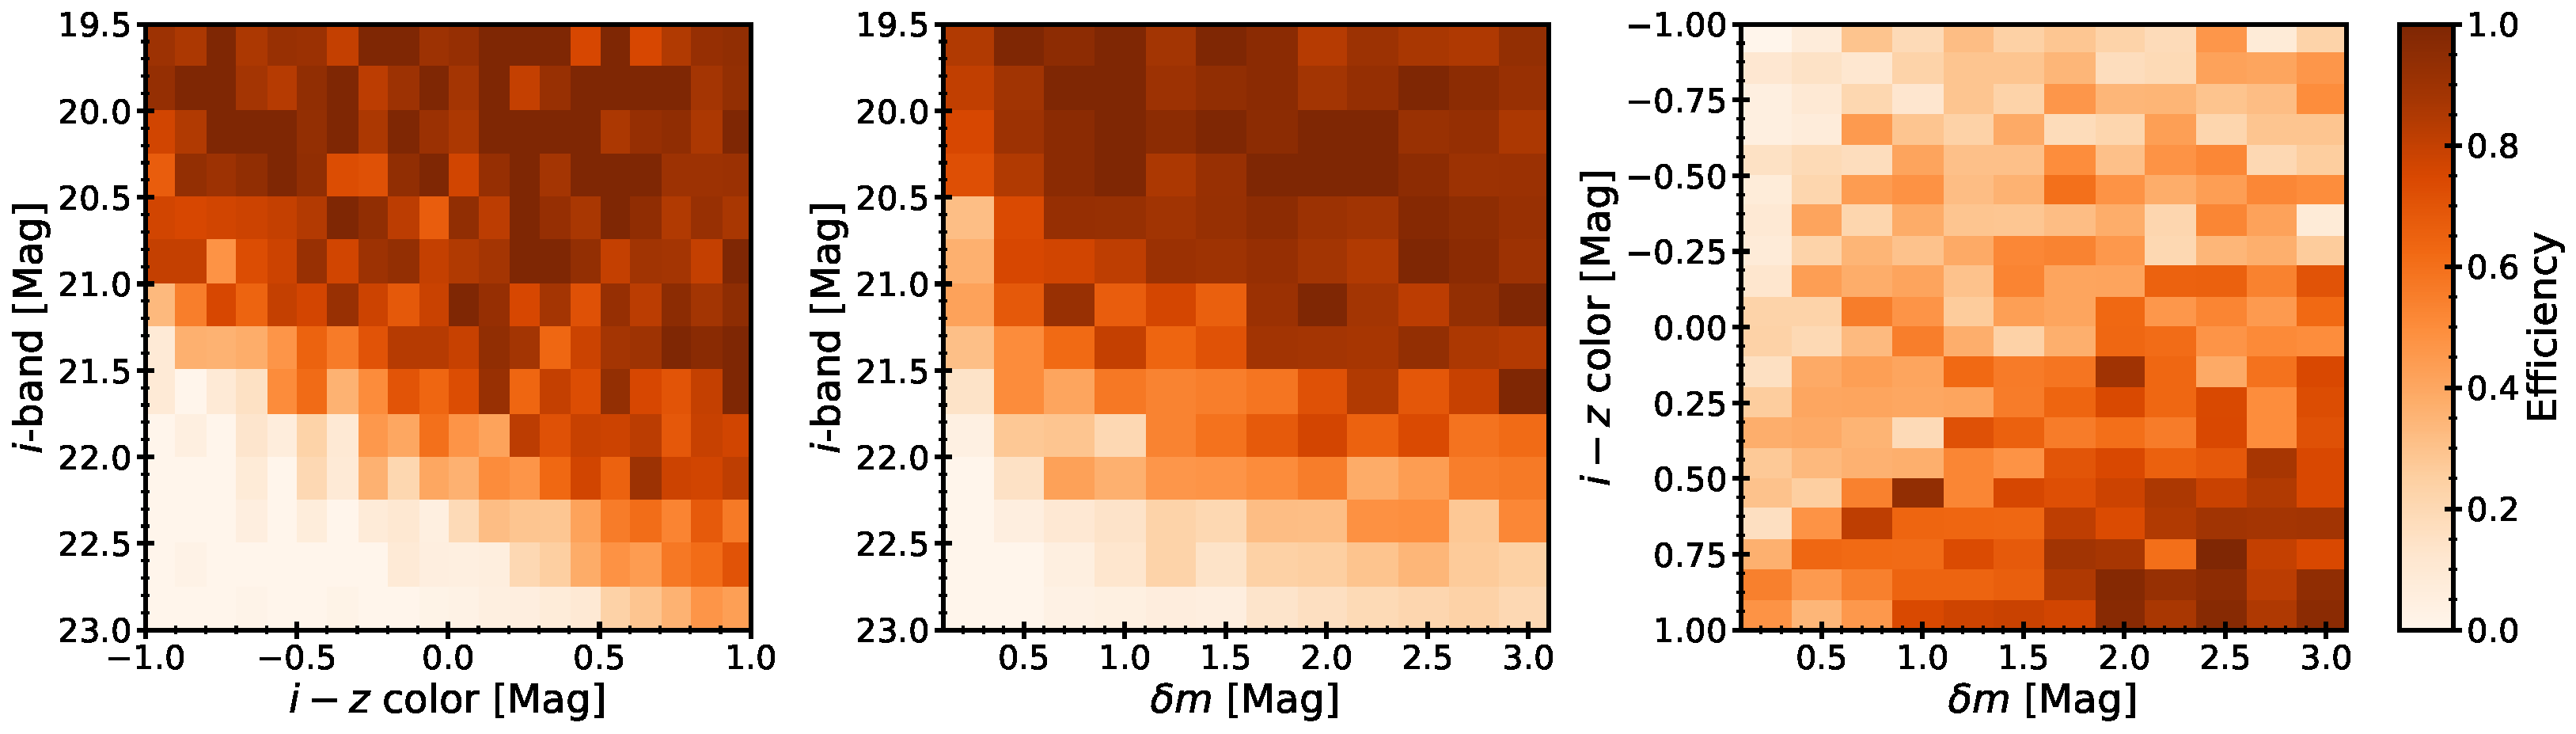
\includegraphics[width=\textwidth]{./figs/chapter3/f7alt.pdf}}
\caption{\singlespace Two dimensional histograms of efficiency. {\it Left:} Efficiency as a function of $i$-band magnitude and $i-z$ color. There is a clear dependence of depth on color, due to the design of our observations. {\it Middle:} Efficiency as a function of $i$-band magnitude and source fading. There is a sharp decline in efficiency for injected sources with a fading of $\lesssim 1$ mag between the search and template images, but otherwise our efficiency is constant above this value. {\it Bottom:} Efficiency as a function of $i-z$ color and source contrast. Our highest efficiency is for sources with red $i-z$ colors and large contrast, the properties expected for red kilonovae.}
\label{fig:ch3_eff_2D}
\end{center}
\end{figure}

We quantify our final efficiencies at a limiting magnitude of $i \lesssim 22.5$ mag, corresponding to the magnitude at which the efficiency for the entire population of fake sources is $\lesssim0.2$. We compute final efficiencies of $\approx90\%$ for red kilonova sources and $\approx60\%$ for blue kilonovae sources.

\clearpage
The initial set of cuts to determine if a fake point source is red or blue kilonova-like are applied to the injected properties, but the measured properties can vary quite significantly. For faint sources ($i \gtrsim 22.5$ mag), the measured color of a source can be inaccurate by $\gtrsim 0.25$~mag and the error does not approach zero until $i  \lesssim 20$ mag. This error in color can lead to a fake source being miscategorized during recovery. We investigate this effect by identifying sources in our sample that would be miscategorized if our analysis was based on the {\it measured} source properties. We find that this is an overall minor effect, leading to a $\lesssim 10 \%$ change to the calculated efficiency.

\section{Contamination Rates}
\label{sec:ch3_contam_rates}
We now combine the results of \cref{sec:ch3_search,sec:ch3_fakes} to compute the areal rate of contaminating sources for the effective sky area for our search ($A_{\rm sky} \approx56$~deg$^2$). We note that our rates are for the relevant ``per search," and not per unit time. These rates can easily be combined with the size of a given GW localization region to compute an expected number of contaminating sources. We first compute the expected detection efficiency relevant for each source in our sample given its color and magnitude; we do not consider the source location relative to a galaxy since our efficiency is uniform with angular separation (\Cref{fig:ch3_eff_1D}). In \Cref{fig:ch3_color_dist_corr} we plot the efficiency-corrected number of sources as a function of $i-z$ color in three bins corresponding to red kilonovae, blue kilonovae, and intermediate colors. We compute $1\sigma$ confidence intervals assuming simple Poisson counting statistics. These confidence intervals are computed for the raw number of sources and are then scaled by the mean efficiency in each color bin.

\begin{figure}[!t]
\begin{center}
\hspace*{-0.1in}
\scalebox{1.}
{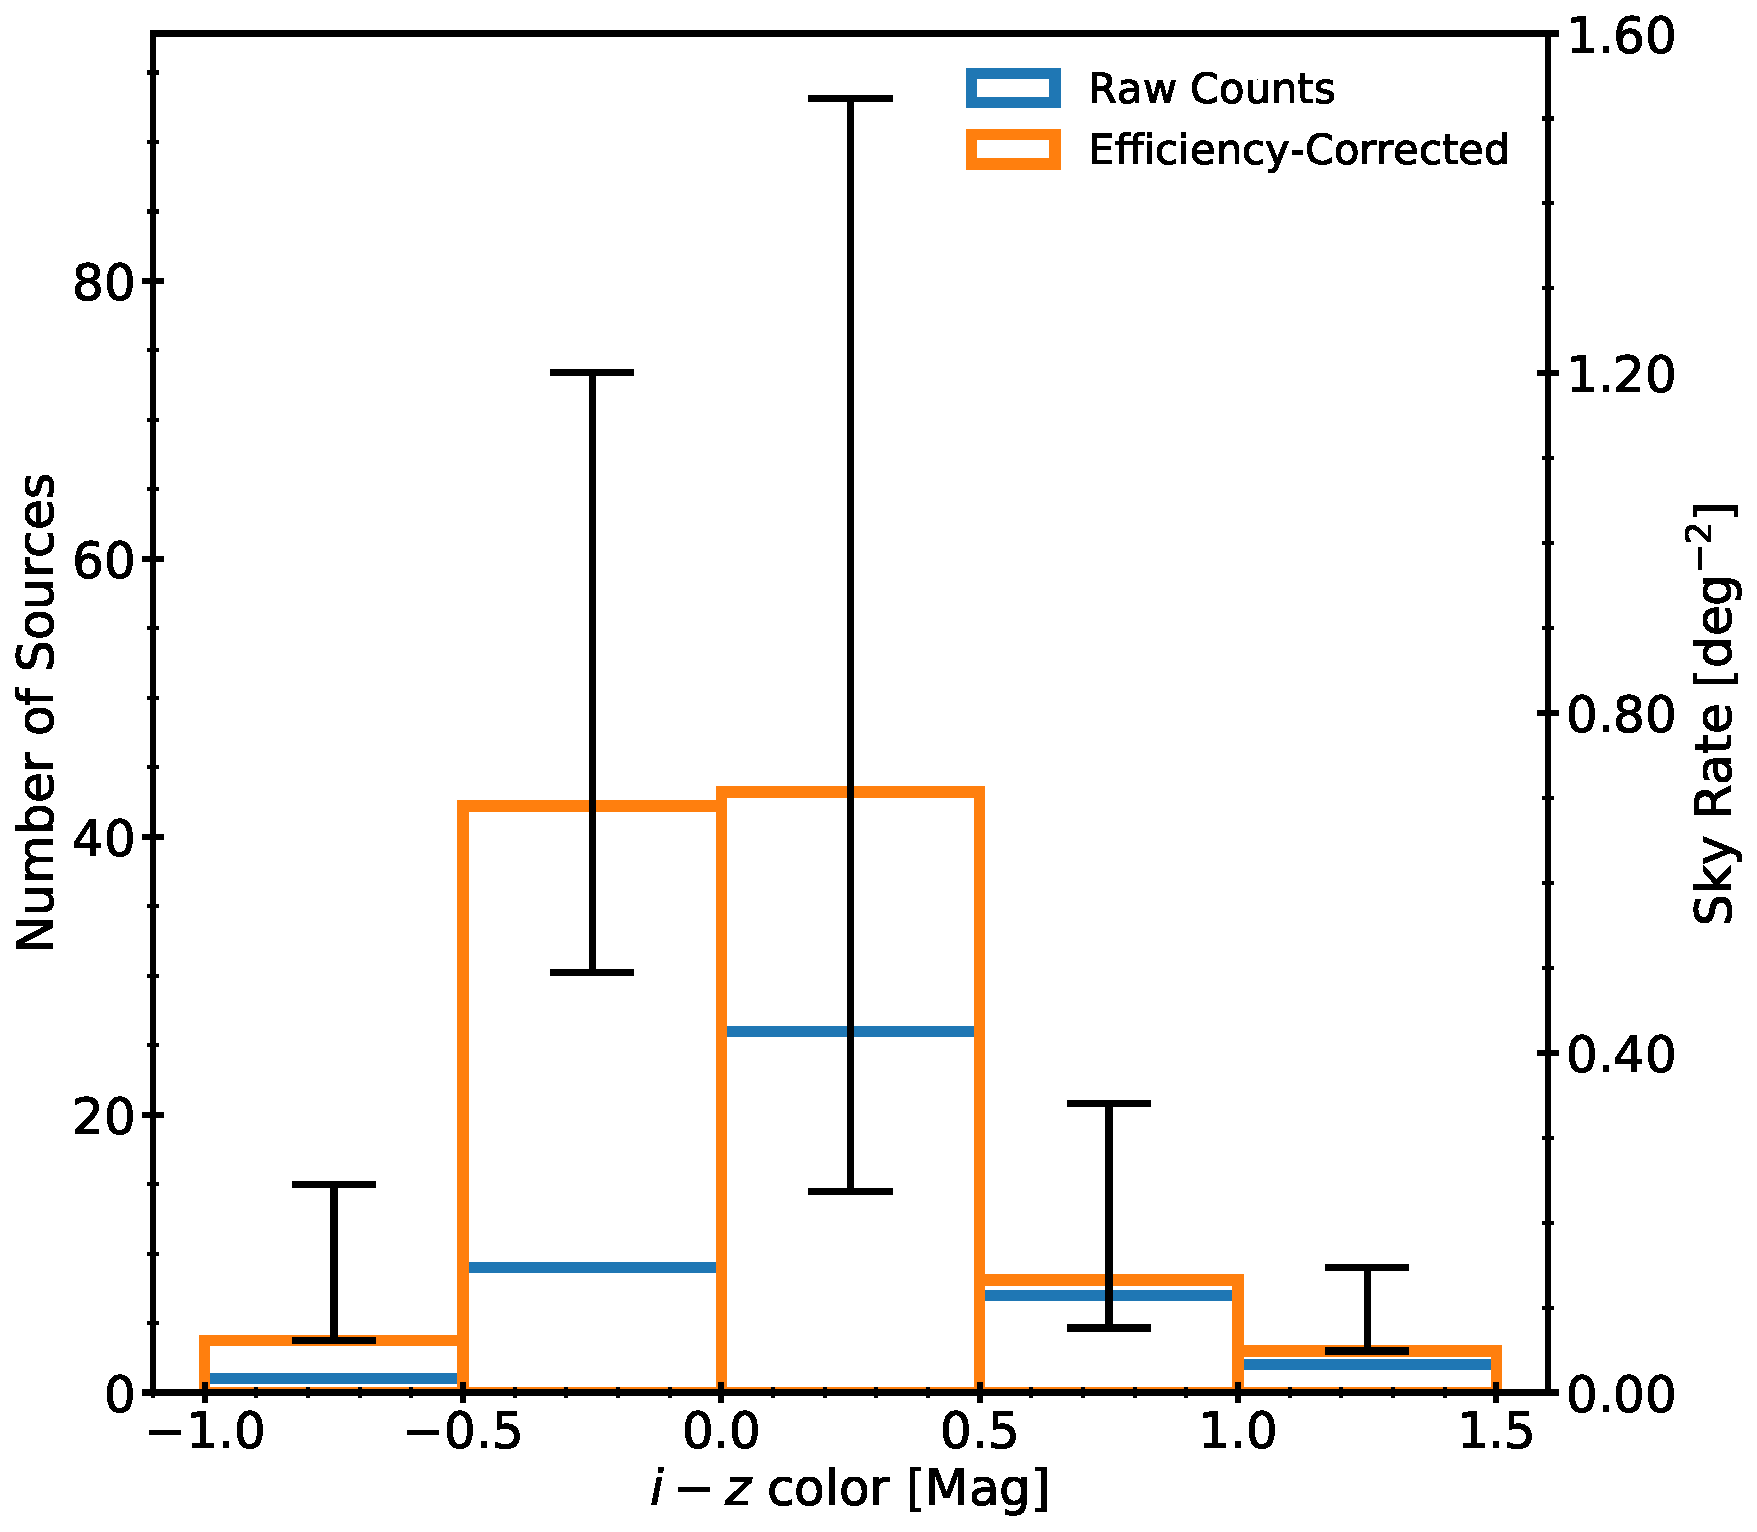
\includegraphics[width=0.9\textwidth]{./figs/chapter3/f8.pdf}}
\caption{\singlespace Histogram of contaminant numbers and areal rates as a function of $i-z$ color. The blue lines indicate the raw source counts, while the orange line indicates the efficiency-corrected counts. The error bars represent the $1\sigma$ confidence interval as computed assuming Poisson counting statistics.}
\label{fig:ch3_color_dist_corr}
\end{center}
\end{figure}

\clearpage
We maintain consistency with our calculated efficiencies from \cref{sec:ch3_fakes} by only considering sources with a mean $i$-band magnitude of $i \lesssim 22.5$~mag as computed from the forced {\tt DoPhot} photometry. At this magnitude limit there are $45$ sources out of the total initial sample of $48$ from \cref{sec:ch3_kn_search}. The magnitude-limited sample of red kilonova contaminants found in \cref{sec:ch3_kn_search} is composed of 9 sources. Correcting for detection efficiency leads to a contaminant rate of 0.16 deg$^{-2}$ at a $5\sigma$ limiting magnitude of $i \lesssim 22.5$ mag. The efficiency-corrected rate of non-nuclear red kilonova contaminants is 0.11 deg$^{-2}$.  For a typical ALV localization region of $\sim 100$ deg$^2$ we therefore expect 16 kilonova contaminants, with about 11 being non-nuclear (at $i\lesssim 22.5$ mag).

For the blue kilonova contaminants all 10 sources are above the magnitude limit. The efficiency corrected number is 46, driven primarily by two sources that are faint ($i \gtrsim 22.2$ mag) and blue ($i-z \approx -0.1$~mag) and therefore have low detection efficiencies of only $\approx 0.1$. If we remove these sources from consideration, then the efficiency-corrected number is 20. There is therefore about a factor of 2 uncertainty in the resulting contamination rate. Considering all sources, the contamination rate is about 0.80 deg$^{-2}$ to a limiting magnitude of $i\approx 22.5$ mag, or $\approx 80$ sources in a $100$ deg$^2$ localization region. The complete set of selections and efficiency-corrected rates are presented in \cref{tab:ch3_cuts_sum}.

We compare the contamination rates derived from our search to those from several follow-up observations of GW sources from the first aLIGO observing run. We focus on optical follow-up using wide-field instruments for GW150914 and
GW151226. Specifically, we use the published results from observations with DECam (\citealt{GW150914DECam,Cowp+16}), the intermediate Palomar Transient Factory (\citealt{Kasliwal+16}), the Kiso Wide-Field Camera (KWFC) used as part of the J-GEMs collaboration (\citealt{Morokuma+16,Yoshida+17}), and the Pan-STARRS/PESSTO/ATLAS search \citep{GW150914PS1,GW151226PS1}. The parameters and results of these searches are summarized in \cref{tab:ch3_O1_sum}.

It is important to note that the searches conducted in response to GW150914 and GW151226 were fundamentally different from our study, as well as from searches that would be required to detect actual kilonovae. These searches employed slow cadences ($\approx \rm few$ days), shallower depths, and did not use colors for source selection. Nevertheless, we can use the numbers of reported transients, which were all deemed unrelated to the GW event, as a proxy for the contamination rate.

We find that our measured contaminant rate, for both red and blue sources, is higher than those reported during O1 follow-up, which had a typical rate of  $\lesssim 0.1$ deg$^{-2}$. However direct comparison requires careful consideration of selection criteria and depth. For example, the iPTF and KWFC follow-up of GW151226 both achieved comparable depth to each other and their reported contaminant rates are in good agreement. By comparison, the DECam and iPTF follow-up of GW150914, both observed the same contamination rate despite the DECam observations being significantly deeper. This is due to a difference in selection criteria as the DECam search focused only on finding rapidly declining transients.


\clearpage
\begin{landscape}
\singlespace
\begin{deluxetable}{c | c c c c | c c c c | c}
\tabletypesize{\footnotesize}
\tablecolumns{10}
\tablewidth{0pt}
\tablecaption{Summary of O1 Optical Follow-Up
\label{tab:ch3_O1_sum}}
\tablehead{
    \colhead{} &
    \multicolumn{4}{|c|}{GW150914} &
    \multicolumn{4}{|c|}{GW151226} &
    \colhead{} \\
    \colhead{Group} &
    \multicolumn{1}{|c}{$m_{5\sigma}$} &
    \colhead{$A_{\rm Sky}$} &
    \colhead{$N$} &
    \multicolumn{1}{c|}{$\mathcal{R}_{\rm sky}$} &
    \multicolumn{1}{|c}{$m_{5\sigma}$} &
    \colhead{$A_{\rm Sky}$} &
    \colhead{$N$} &
    \multicolumn{1}{c|}{$\mathcal{R}_{\rm sky}$} &
    \colhead{Notes} \\
    \colhead{} &
    \multicolumn{1}{|c}{(Mag)} &
    \colhead{(deg$^2$)} &
    \colhead{(Number)} &
    \multicolumn{1}{c|}{(deg$^{-2}$)} &
    \multicolumn{1}{|c}{(Mag)} &
    \colhead{(deg$^2$)} &
    \colhead{(Number)} &
    \multicolumn{1}{c|}{(deg$^{-2}$)} &
    \colhead{}
}
\startdata
DECam & $i \lesssim 22.5$ & 102 & 9 &  0.08 & $i \lesssim 21.7$ & 28.8 & 4 & 0.13 & {\it A} \\
iPTF & $r \lesssim 20.5$ & 126 & 8 & 0.06 & $r \lesssim 20.5$ & 731 & 21 & 0.03 & {\it B} \\
J-GEM/KWFC  & $i \lesssim 18.9$ & 24 & 0 & $\lesssim0.13$ & $r \lesssim 20.5$ &  778 & 13 & 0.02 & {\it C} \\
Pan-STARRS & $i \lesssim 20.8$ & 442 & 56 & 0.12 & $ i \lesssim 20.8$ & 290 & 49 & 0.17 & {\it D} \\
\enddata
\tablecomments{Summary of optical follow-up for the two high-signficance GW events detected during
the first aLIGO observing run \citep[O1;][]{LIGOGW150914FollowUp, LIGOGW150914FollowUpSupp}. We report the published limiting magnitude $(m_{5\sigma})$, the area covered
($A_{\rm sky}$), the number of reported candidates $(N)$, and the projected sky rate $(\mathcal{R} \equiv N / A_{\rm sky})$.}
\tablenotetext{A }{~References: \cite{GW150914DECam,Cowp+16}}
\tablenotetext{B }{~References: \cite{Kasliwal+16}}
\tablenotetext{C }{~References: \cite{Morokuma+16,Yoshida+17} \\
Note: Here we only consider the KWFC wide-field survey component of the J-GEM follow-up.}
\tablenotetext{D }{~References: \cite{GW150914PS1,GW151226PS1}}
\end{deluxetable}
\end{landscape}

It is critical to note that while our measured contamination rate is higher, the observations used in this work were conducted at the depths and cadences necessary for searches targeting kilonovae. Therefore, the rates derived here are more relevant for GW follow-up conducted in response to BNS and NS-BH mergers.

\subsection{Rates for Short Timescale Transients}
\label{sec:ch3_rates_short}

We also compute expected contamination rates for sources identified in our short timescale search (\cref{sec:ch3_kn_short}). For both the $\approx 3-24$ hr and $\lesssim 3$ hr timescales we did not identify any credible source of extragalactic contamination. This leads to an efficiency-corrected upper limit of $\lesssim 0.07$ deg$^{-2}$ (95\% confidence level) at $i\approx 22.5$ mag for both populations. A $100$ deg$^2$ GW localization region would therefore contain $\lesssim 7$ contaminants on these timescales. These rates are included in \cref{tab:ch3_cuts_sum}.

These rates can be compared to the Pan-STARRS1 Medium-Deep Survey fast transients search of \cite{Berger+13}. That study focused on a timescale of $\sim 0.5$ hr to $\sim 1$ d and led to an upper limit on the rate of extragalactic transients of $\lesssim 2.4\times 10^{-3}$ deg$^{-2}$ day$^{-1}$ for the timescale of 1 d, and $\lesssim 0.12$ deg$^{-2}$ day$^{-1}$ for a timescale of 0.5 hr at a limiting magnitude of $r\approx 22.4$ mag. For our search (56 deg$^2$ and 4 d) we therefore expect $\lesssim 0.5$ events on a timescale of $\lesssim 1$ d, consistent with our non-detection of any extragalactic contaminants.

\section{Discussion and Conclusions}
\label{sec:ch3_conc}
We presented an empirical study of contamination rates in rapid, deep, wide-field optical follow-up of GW sources. Our observations used DECam to cover a wide search area of $56$ deg$^2$ and to probe the regime applicable for kilonovae at expected BNS merger detection distances.  We also explored timescales ranging from $\sim 3$ hours (applicable for a neutron precursor signal) to several days (applicable to blue and red kilonova emission). We search the data for transient sources that would contaminate searches for red kilonova emission, blue kilonova emission, or a neutron precursor.  We note that the former is a robust prediction of BNS mergers, while the latter two are more speculative and depend on currently unknown factors such as the neutron star equation of state. The key results of our study are as follows:

\begin{enumerate}
\item We find 48 transient sources coincident with galaxies, and lacking a point source in the template images.  Furthermore, we find 14 transients with point source counterparts that exhibit stellar colors, but are too faint to be present in catalogs such as Gaia DR1.  These sources can be rejected as contaminants under most circumstances, but may confuse real-time searches if pre-existing templates are not available.

\item We use $i-z$ color selection for the 48 sources to identify contaminants for red and blue kilonovae \citep{BarnesKasen13,Kasen+15}. We find 11 red kilonova ($i-z \gtrsim 0.5$~mag) and 10 blue kilonova ($i-z < 0$~mag) contaminants.

\item We search the data for transients with a timescale of $\lesssim 1$ d, which will contaminate searches for a ``neutron precursor" signal.  We identify no credible evidence for extragalactic contamination on these timescales.

\item We compute efficiency-corrected areal rates for contaminants (per GW follow-up search) at a limiting magnitude of $i\approx 22.5$ mag, of $\mathcal{R}_{\rm tot}\approx 1.79$ deg$^{-2}$, $\mathcal{R}_{\rm red}\approx 0.16$ deg$^{-2}$, and $\mathcal{R}_{\rm blue}\approx 0.80$ deg$^{-2}$. We compute an upper limit areal rate for sources with a characteristic timescale of $\lesssim 1$ day of $\lesssim 0.07$ deg$^{-2}$ at the 95\% confidence level.

\item Our derived contamination rates are higher than reported optical transients found in follow-up of GW150914 and GW151226 ($\mathcal{R} \approx 0.1$ deg$^2$), but this is due to the greater depth of our observations, which are better matched to kilonova detections (CB15).
\end{enumerate}

We also consider our search criteria as they relate to the optical transient associated with GW170817. This counterpart would have easily passed all of our initial cuts (e.g., strictly positive flux, 4 detections at SNR $>$ 5) and been placed in Group 2 as a bright point source near an obvious host galaxy. However, it would not have passed any color cuts (e.g., $i-z > 0.5$~mag.). Nevertheless, manual inspection would quickly reveal this source to be new, genuine, and worthy of further follow-up. However, as stated previously, several of the circumstances associated with GW170817 (e.g., relatively local, bright, obvious host galaxy) are unlikely to be the case for future detections. Therefore, the unique nature of this discovery should not strongly impact future follow-up strategies.

In the context of future searches with three GW detectors (ALV), the typical localization regions are $\lesssim 100$ deg$^2$. At design sensitivity, about half of all BNS mergers are expected to be localized to $\lesssim10$ deg$^2$ \citep{ChenHolz16}. Similarly, with a five-detector network (ALV+KAGRA+LIGO India) it is expected that \apx90\% of BNS mergers will be localized to $\lesssim 10$ deg$^2$ \citep{ChenHolz16}. Based on our derived rates, we expect such regions to contain a few contaminants. However, we note that the depth of our search is valid for detecting kilonovae out to a luminosity distance of \apx100 Mpc. Detecting kilonovae out to the aLIGO BNS horizon at design sensitivity ($\sim200$ Mpc) requirs our search to go a magnitude deeper, increasing the expected contamination by a factor of four if we assume Euclidean volume scaling and uniform source distribution.

The challenge of contamination in deep follow-up of GW triggers is significant, but not insurmountable. If localization regions can be reduced to \apx100--200 deg$^2$, we would expect to find \apx170--340 contaminants during a typical search, before making any color cuts. The most aggressive cut, looking for red and non-nuclear sources, would reveal \apx11--22 contaminants in \apx100--200 deg$^2$ localization regions. Obtaining follow-up photometry and NIR spectroscopy for this number of sources, at magnitudes of $z \gtrsim 21$~mag, is a difficult task requiring the allocation of dedicated time on 8-m class telescopes. Looking ahead to the era of $\lesssim 10$ deg$^2$, even our broadest selection criteria will yield fewer than $\sim 10$ candidates. In this regime, obtaining rapid NIR spectroscopic follow-up of sources to assess their true nature becomes tractable and we will truly enter the next generation of multi-messenger astronomy.

% NOTE THE LACK OF A BIBLIOGRAPHY CALL IN THIS FILE. BIBLIOGRAPHY WORK HAPPENS OUTSIDE THE CHAPTER TEX FILES.

\clearpage
%
\chapter{Chapter 4 Title}\label{c:occ}
\chaptermark{Short Chapter 4 Title}
\begin{quote}
{\em ~~~~~~~This thesis chapter originally appeared in the literature as} \\
{authors,
{\em journal reference info}}
\end{quote}
%UNLIKE IN A REGULAR TEX FILE, DON'T PUT ANY PREAMBLE MATERIAL HERE

\section*{Abstract}
  We report the results of a Dark Energy Camera (DECam)
  optical follow-up of the gravitational wave (GW) event GW151226,
  discovered by the Advanced LIGO detectors. Our observations cover 28.8
  deg$^2$ of the localization region in the $i$ and $z$ bands (containing 3\%
  of the {\tt BAYESTAR} localization probability), starting 10 hours after the
  event was announced and spanning four epochs at $2-24$ days after the
  GW detection. We achieve $5\sigma$ point-source limiting
  magnitudes of $i\approx21.7$ and $z\approx21.5$, with a scatter
  of $0.4$~mag, in our difference images. Given the two day delay,
  we search this area for a rapidly declining optical counterpart with
  $\gtrsim 3\sigma$ significance steady decline between the first and final
  observations. We recover four sources that pass our selection criteria,
  of which three are cataloged AGN. The fourth source is offset
  by $5.8$ arcsec from the center of a galaxy at a distance of 187
  Mpc, exhibits a rapid decline by $0.5$ mag over $4$ days,
  and has a red color of $i-z\approx 0.3$ mag. These properties roughly match
  the expectations for a kilonova. However, this source
  was detected several times, starting $94$ days prior to GW151226,
  in the Pan-STARRS Survey for Transients (dubbed as PS15cdi) and
  is therefore unrelated to the GW event. Given its long-term
  behavior, PS15cdi is likely a Type IIP supernova that
  transitioned out of its plateau phase during our
  observations, mimicking a kilonova-like behavior. We comment on
  the implications of this detection for contamination in future
  optical follow-up observations.

\section{Introduction}
\label{sec:ch4_intro}

The Advanced Laser Interferometer Gravitational-Wave Observatory
(LIGO) is designed to detect the final inspiral and
merger of compact object binaries comprised of neutron stars (NS)
and/or stellar-mass black holes (BH) \citep{LIGOMainRef}.
The first LIGO observing run (designated O1)
commenced on 18 September 2015 with the ability to detect binary
neutron star (BNS) mergers to an average distance of $\sim 80$ Mpc, a
forty-fold increase in volume relative to the previous generation of
ground-based GW detectors. On 2015 September 14 LIGO detected
the first GW event ever observed, GW150914 \citep{LIGOGW150914}.

The waveform of GW150914 was consistent with the inspiral, merger,
and ring-down of a binary black hole (BBH) system ($36+29$ M$_\odot$;
\citealt{LIGOGW150914}) providing the first observational
evidence that such systems exist and merge. While there are no robust
theoretical predictions for the expected electromagnetic (EM)
counterparts of such a merger, more than 20 teams conducted a wide
range of follow-up observations spanning from radio to $\gamma$-rays, along with neutrino follow up
\citep{LIGOGW150914FollowUp,LIGOGW150914FollowUpSupp,GW150914IceCube,Annis+16,GW150914Fermi,Evans+16,Kasliwal+16,Savchenko+16,GW150914PS1,GW150914DECam,Tavani+16}.
This effort included deep optical follow-up observations by our group using DECam covering 100 deg$^2$
(corresponding to 38\%~(11\%) of the initial~(final) sky maps)
 -- making this one of the most comprehensive optical
follow-up campaigns for GW150914 \citep{Annis+16,GW150914DECam}. Our search for rapidly
declining transients to limiting magnitudes of $i\approx21.5$ mag
for red $(i-z=1)$ and $i\approx20.1$ mag for blue $(i-z=-1)$ events yielded no counterpart to
GW150914 \citep{GW150914DECam}. One result of the broader multi-wavelength
follow-up campaign is a claimed coincident detection of a weak short
gamma-ray burst (SGRB) from the {\it Fermi}/GBM detector 0.4 s after
the GW event \citep{GW150914Fermi}. However, this event was not
detected in INTEGRAL $\gamma$-ray data \citep{Savchenko+16} and was also
disputed in a re-analysis of the GBM data \citep{Greiner+16}.

A second high-significance GW event, designated GW151226, was
discovered by LIGO on 2015 December 26 at 03:38:53 UT \citep{LIGOGW151226}.
This event was also due to the inspiral and merger of a BBH system, consisting
of $14.2^{+8.3}_{-3.7}$~M$_\odot$ and $7.5^{+2.3}_{-2.3}$~M$_\odot$ black holes at a luminosity
distance of $d_L = 440^{+180}_{-190}$~Mpc \citep{LIGOGW151226}.
The initial localization was provided as a probability sky map via a private
GCN circular 37 hours after the GW detection \citep{SingerPrice16}. We initiated
optical follow-up observations with DECam 10 hours later on 2015 December 28,
and imaged a 28.8 deg$^2$ region in the $i$ and $z$ bands during several epochs. Here we report
the results of this search. In \cref{sec:ch4_obs} we discuss the
observations and data analysis procedures. In \cref{sec:ch4_analysis}
we present our search methodology for potential counterparts to GW151226,
and the results of this search. We summarize our conclusions in \cref{sec:ch4_conc}. We perform
cosmological calculations assuming $H_0 = 67.8$~km  s$^{-1}$ Mpc$^{-1}$,
$\Omega_{\lambda} = 0.69$, and $\Omega_m = 0.31$ \citep{Planck2016}.
 Magnitudes are reported in the AB system.

\clearpage
\section{Observations and Data Reduction}
\label{sec:ch4_obs}

GW151226 was detected on 2015 December 26 at 03:38:53 UT by a
Compact Binary Coalescence (CBC) search pipeline \citep{LIGOGW151226}. The CBC
pipeline operates by matching the strain data against waveform
templates and is sensitive to mergers containing NS and/or BH.
The initial sky map was generated by the {\tt BAYESTAR} algorithm
and released 37 hours after the GW detection. {\tt BAYESTAR} is a Bayesian
algorithm that generates a localization sky map based on the parameter
estimation from the CBC pipeline \citep{Singer+14,SingerPrice16}. The sky area contained within the
initial 50\% and 90\% contours was 430 deg$^2$ and 1340 deg$^2$,
respectively. A sky map generated by the {\tt LALInference}
algorithm, which computes the localization using Bayesian forward-modeling
of the signal morphology \citep{Veitch+15}, was released on 2016 January 15 UT,
after our DECam observations had been concluded. The {\tt LALInference} sky map
is slightly narrower than the sky map from {\tt BAYESTAR} with 50\% and 90\% contours
of 362 deg$^2$ and 1238 deg$^2$, respectively.

We initiated follow-up observations with DECam on 2015 December 28 UT,
two days after the GW detection and 10 hours after distribution of the {\tt BAYESTAR}
sky map. DECam is a wide-field optical imager with a 3 deg$^2$ field of view
\citep{Flaugher+15}. We imaged a 28.8 deg$^2$ region corresponding to 3\%
of the sky localization probability when convolved with the initial {\tt BAYESTAR} map
and 2\% of the localization probability in the final {\tt LALInference} sky map.
The pointings and ordering of the DECam observations were determined using
the automated algorithm described in \citet{GW150914DECam}. The choice
of observing fields was constrained by weather, instrument availability, and the available
time to observe this sky region given its high airmass. We
obtained four epochs of data with each epoch consisting of one 90 s
exposure in $i$-band and two 90 s exposures in $z$-band for each of the 12 pointings. The first
epoch was obtained 2--3 days after the initial LIGO trigger (2015
December 28--29 UT), the second epoch was at 6 days (2016 January 1
UT), the third epoch was at 13--14 days (2016 January 8--9), and the
fourth epoch was at 23--24 days (2016 January 18--19). A summary of
the observations is provided in \cref{ch4_datatable} and a visual
representation of the sky region is shown in
\Cref{fig:ch4_obs}.

\begin{deluxetable}{lrccccccc}
\singlespace
\tabletypesize{\footnotesize}
\tablecolumns{9}
\tablewidth{0pt}
\tablecaption{Summary of DECam Observations of GW151226
\label{ch4_datatable}}
\tablehead{
\colhead{Visit}    &
\colhead{UT}       &
\colhead{$\Delta t$\tablenotemark{a}} &
\colhead{$\langle$PSF$_i$$\rangle$}    &
\colhead{$\langle$PSF$_z$$\rangle$}    &
\colhead{$\langle$airmass$\rangle$}  &
\colhead{$\langle$depth$_i\rangle$}   &
\colhead{$\langle$depth$_z\rangle$}  &
\colhead{$A_{\mathrm{eff}}$\tablenotemark{b}} \\
\colhead{ } &
\colhead{ } &
\colhead{(days)} &
\colhead{(arcsec)} &
\colhead{(arcsec)} &
\colhead{ } &
\colhead{(mag)} &
\colhead{(mag)} &
\colhead{(deg$^2$)}
}
\startdata
 Epoch 1 & 2015-12-28.11 & 1.96 & 0.97 & 0.99 & 1.95 & 22.39 & 22.23 & 14.4 \\      %  6 hexes
               & 2015-12-29.11 & 2.96 & 1.00 & 0.97 & 1.78 & 22.57 & 22.46 & 14.4 \\      %  6 hexes

 Epoch 2 & 2016-01-01.06 & 5.91 & 0.95 & 0.90 & 1.57 & 21.37 & 21.06 & 28.8 \\      % 12 hexes

 Epoch 3 & 2016-01-08.11 & 12.96 & 1.68 & 1.62 & 2.15 & 22.09 & 21.70 & 24.0 \\      % 10 hexes
                & 2016-01-09.11 & 13.96 & 1.17 & 1.12 & 1.80 & 22.44 & 22.17 &  4.8 \\      %  2 hexes

 Epoch 4 & 2016-01-18.03 & 22.88 & 1.21 & 1.20 & 1.48 & 22.00 & 22.01 & 12.0 \\      %  5 hexes
               & 2016-01-19.01 & 23.86 & 1.29 & 1.25 & 1.71 & 21.86 & 21.90 & 16.8 \\ %  7 hexes
\enddata
\tablecomments{Summary of our DECam follow-up observations of
GW151226. The PSF, airmass, and depth are the average values across
all observations on that date. The reported depth corresponds to the mean
$5\sigma$ point source detection in the coadded search images.}
\tablenotetext{a}{Time elapsed between the GW trigger time and the time of the first image.}
\tablenotetext{b}{The effective area corresponds to 12 DECam pointings
taking into account that $\approx 20\%$ of the 3
deg$^2$ field of view of DECam is lost due to chip gaps (10\%), 3
dead CCDs (5\%, \citealt{Diehl+14}), and masked edge pixels (5\%).}
\end{deluxetable}

\begin{figure}[t!]
\centering
\vspace{-60pt}
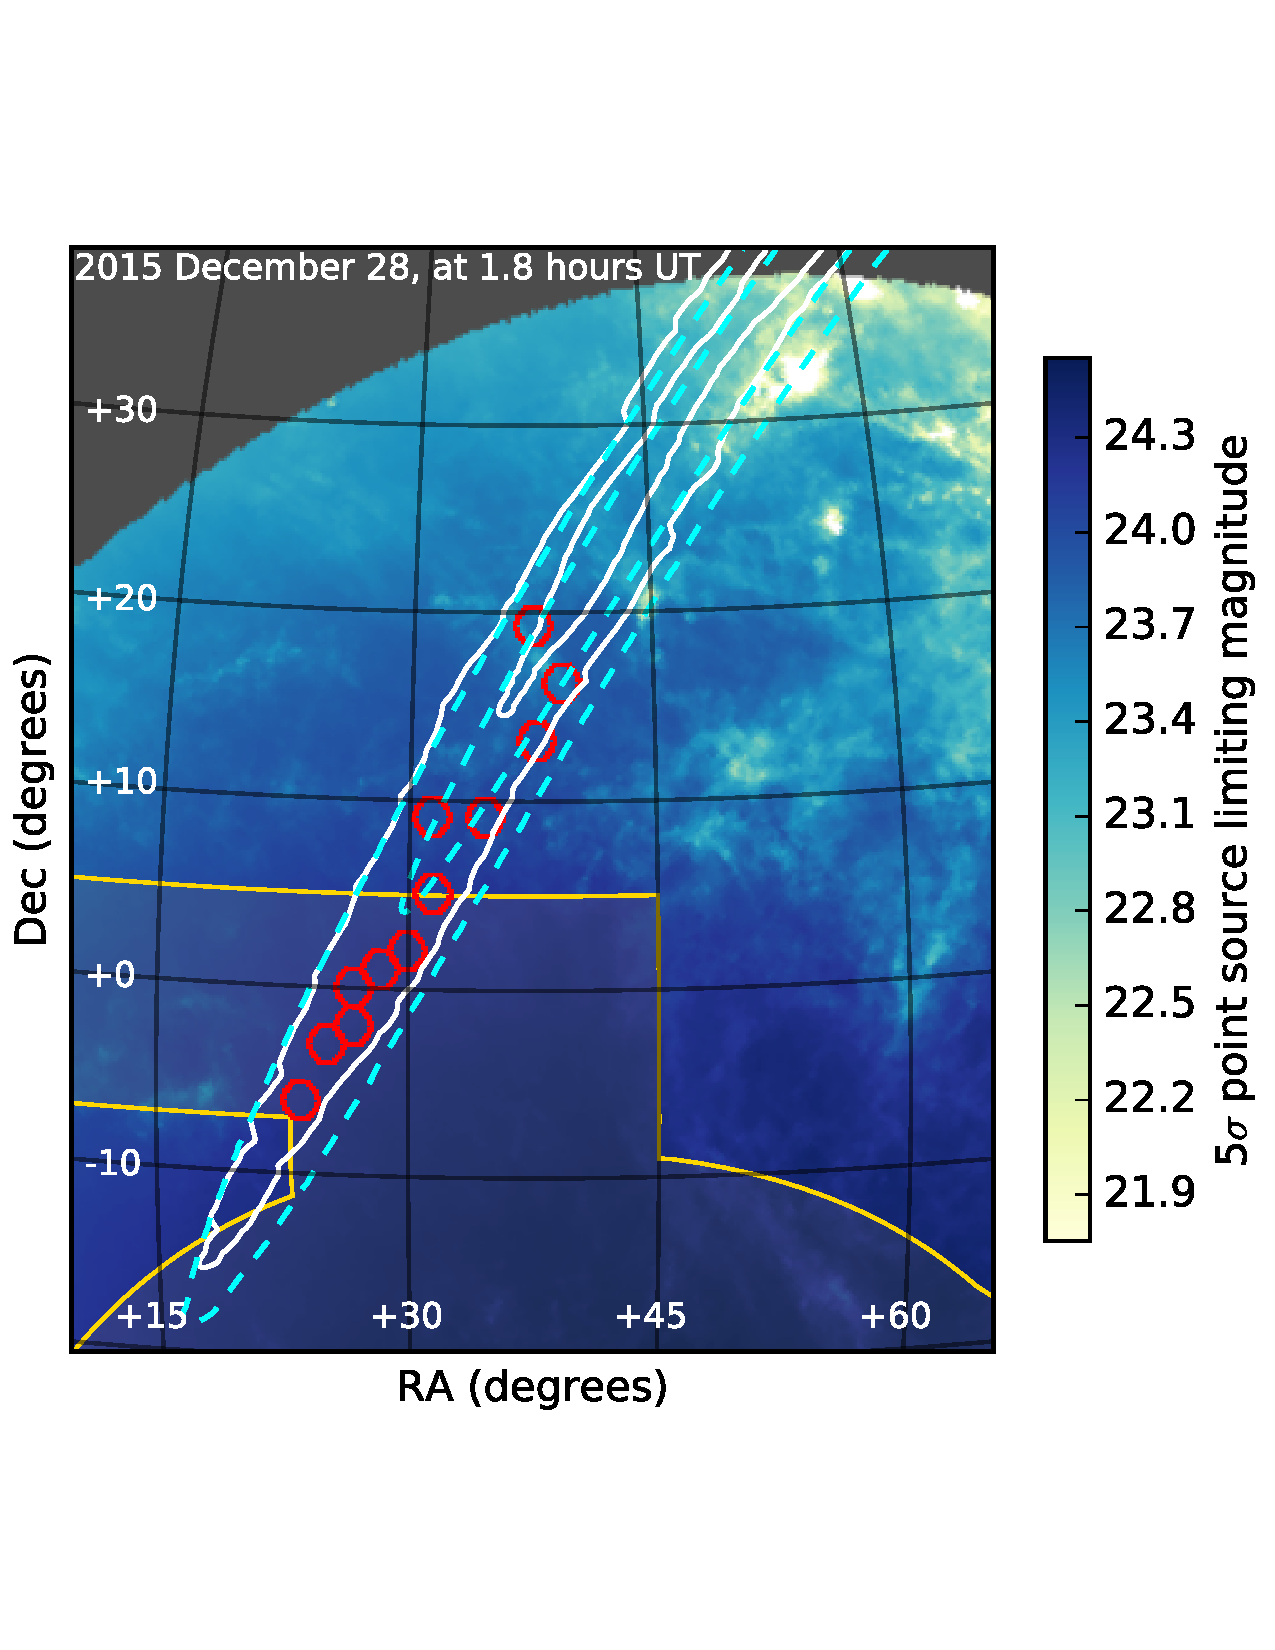
\includegraphics[width=0.75 \textwidth]{./figs/chapter4/fig1.pdf}
\vspace{-60pt}
\caption{\singlespace 
Sky region covered by our DECam observations (red
hexagons) relative to the 50\% and 90\% probability regions
from the {\tt BAYESTAR} (cyan contours) and {\tt LALInference}
(white contours) localization of GW151226.
The background color indicates the estimated $5\sigma$
point-source limiting magnitude for a 90~s $i$-band exposure
as a function of sky position for the first night of our DECam
observations. The variation in the limiting magnitude is largely
driven by the dust extinction and airmass at that position.
The dark grey regions indicate sky positions that
were unobservable due to the telescope pointing limits.  The yellow contour
indicates the region of sky covered by the Dark Energy Survey
(DES). The total effective area for the 12 DECam pointings is 28.8
deg$^2$, corresponding to 3\%~(2\%) of the probability in the
{\tt BAYESTAR}~({\tt LALInference}) sky map.}
\label{fig:ch4_obs}
\end{figure}

We processed the data using an implementation of the {\tt photpipe}
pipeline modified for DECam images. {\tt Photpipe} is a
pipeline used in several time-domain surveys (e.g.,
SuperMACHO, ESSENCE, Pan-STARRS1; see \citealt{Rest+05,Garg+07,Miknaitis+07,Rest+14}), designed to perform
single-epoch image processing including image calibration (e.g., bias
subtraction, cross-talk corrections, flat-fielding), astrometric
calibration, image coaddition, and photometric calibration.
Additionally, {\tt photpipe} performs difference imaging using {\tt
  hotpants} \citep{Alard2000,Becker2015} to compute a spatially varying convolution kernel,
followed by photometry on the difference images using an
implementation of {\tt DoPhot} optimized for point spread function (PSF) photometry on
difference images \citep{Schechter+93}. Lastly, we
use {\tt photpipe} to perform initial candidate searches by
specifying a required number of spatially coincident detections over a
range of time. Once candidates are identified, {\tt photpipe} performs
``forced" PSF photometry on the subtracted images at the fixed coordinates of
an identified candidate in each available epoch.

\clearpage
In the case of the GW151226 observations, we began with raw images
acquired from the NOAO archive\footnote{\singlespace http://archive.noao.edu/} and the
most recent calibration files\footnote{\singlespace http://www.ctio.noao.edu/noao/content/decam-calibration-files}.
Astrometric calibration was performed relative to the Pan-STARRS1 (PS1)
$3\pi$ survey and 2MASS $J$-band catalogs. The two $z$-band exposures
were then coadded. Photometric calibration was performed using the
PS1 $3\pi$ survey with appropriate calibrations between
PS1 and DECam magnitudes \citep{Scolnic+15}. Image subtraction was performed
using observations from the final epoch as templates. The approach
to candidate selection is described in \cref{sec:ch4_analysis}.

Our observations achieved average $5\sigma$ point-source limiting
magnitudes of $i\approx22.2$ and $z\approx21.9$ in the coadded single-epoch
search images, and $i\approx21.7$ and $z\approx21.5$ in the difference
images, with an epoch-to-epoch scatter of 0.4 mag. The variability in
depth is driven by the high airmass and
changes in observing conditions, particularly during the second epoch.

\section{Search for an Optical Counterpart}
\label{sec:ch4_analysis}

The primary focus of our search is a fast-fading transient.
While the merger of a BBH system is not expected
to produce an EM counterpart, it is informative to consider the
possibility of optical emission due to the presence of some matter in
the system. As a generic example, we consider the behavior of a
transient such as a short gamma-ray burst (SGRB) with a typical beaming-corrected energy of
$E_j \approx 10^{49}$ erg and an opening angle of $\theta_j\approx
10^\circ$ \citep{Berger2014,Fong+15}. If viewed far off-axis $(\theta_{\rm
  obs}\gtrsim 4\theta_j)$ the optical emission will reach peak
brightness after several days, but at the distance of GW151226
($\approx440$ Mpc, \citealt{LIGOGW151226}), the peak brightness will be $i\approx 26$ mag (see Figure 5 of
\citealt{MetzgerBerger12}), well beyond our detection limit. If the source
is observed moderately off-axis or on-axis $(\theta_{\rm obs} \lesssim
2\theta_j)$, then the light curve will decline throughout our
observations, roughly as $F_\nu\propto t^{-1}$, and will be detectable
at $i\approx$ 21--22 mag in our first observation (see Figures 3 and 4
of \citealt{MetzgerBerger12}). We can apply a similar argument to the
behavior of a more isotropic (and non-relativistic) outflow given that
any material ejected in a BBH merger is likely to have a low mass and
the outflow will thus become optically thin early, leading to fading
optical emission. Based on this line of reasoning, we search our data
for steadily declining transients.

We identify relevant candidates in the data using the following
selection criteria with the forced photometry from {\tt
  photpipe}. Unless otherwise noted these criteria are applied to
  the $i$-band data due to the greater depth in those observations.

\begin{enumerate}

\item We require non-negative or consistent with zero
(i.e., within 2$\sigma$ of zero)
$i$- and $z$-band fluxes in the difference photometry
across all epochs to eliminate any sources that re-brighten in the
template epoch. This provides an initial sample of 602 candidates.

\item We require $\ge 5\sigma$ $i$- and $z$-band detections in the
first epoch and at least one additional $\ge 5\sigma$ $i$-band
detection in either of the two remaining epochs (to eliminate contamination
from asteroids). This criterion leaves a sample of 98 objects.

\clearpage
\item We require a $\ge 3\sigma$ decline in flux between the first and
third epochs to search for significant fading\footnote{\singlespace We note that this
criterion effectively requires the detection in the first epoch to be $\gtrsim 5\sigma$
producing an effectively shallower transient search. Soares-Santos et al.
\citeyearpar{GW150914DECam} quantified this effect by injecting fake sources into
their observations to determine the recovery efficiency and loss of detection
depth from analysis cuts. Here, we forego
such analysis to focus the discussion on the effects of contamination in
optical follow-up of GW events.}. We calculate $\sigma$ as the
quadrature sum of the flux errors from the first and third epochs
($\sigma = \sqrt{\sigma_1^2 + \sigma_3^2}$, where $\sigma_1$ and
$\sigma_3$ are the flux errors from the first and third epochs,
respectively). This criterion leaves a sample of 48 objects.

\item We reject sources that exhibit a significant ($\ge 3\sigma$) rise in flux
between the first and second epochs or the second and third epochs to eliminates variable
sources that do not decline steadily. This criterion leaves a sample of 32 objects.

\item We reject sources that are present as an isolated point source in
the fourth (template) epoch to eliminate variable stars. This step involved
visual inspection of the 32 candidates from step 4.

\end{enumerate}

Only four events passed our final criterion. We find that two of those events are
coincident with the nuclei of known AGN (PKS\,0129-066 and Mrk\,584), indicating
that they represent AGN variability. A third candidate is coincident with the nucleus of
the bright radio source PMN\,J0203+0956 ($F_\nu(365\,{\rm MHz})\approx 0.4$ Jy,
\citealt{Douglas+96}), also suggesting AGN variability.

\clearpage
The final candidate in our search is located at RA = 01$^{\rm h}$42$^{\rm m}$16$^{\rm s}$.17 and DEC = $-$02\arcdeg13\arcmin42 6\arcsec~(J2000), with an offset of $5.8$ arcsec from the galaxy CGCG 386-030 (RA =  01$^{\rm h}$42$^{\rm m}$15$^{\rm s}$.6, DEC = $-$02\arcdeg13\arcmin38 5\arcsec; J2000), at $z = 0.041$ or $d_L \approx 187$ Mpc (6dFGS, \citealt{Jones+04,Jones+09}); see \Cref{fig:ch4_PS15cdi}. We note that this distance is inconsistent with the 90\% confidence interval for the distance to GW151226 based on the GW data \citep{LIGOGW151226}. We observe this source in a state of rapid decline with an absolute magnitude of $M_i \approx -15$~mag on 2015 December 28 and $M_i\approx -14.5$~mag on 2016 January 1, indicating a decline rate of $\approx 0.12$ mag d$^{-1}$; the decline rate in $z$-band is $\approx 0.10$ mag d$^{-1}$. Additionally, the source exhibits a red $i-z$ color of $0.3$ mag.

We fit these data to a power-law model typical for GRB afterglows $(F_\nu \propto \nu^{\beta} t^{\alpha})$ and find a temporal index of $\alpha = -0.43\pm0.12$ and a spectral index of $\beta = -1.8\pm0.8$, both of which differ from the expected values for GRB afterglows ($\alpha \approx -1$, $\beta \approx -0.75$, \citealt{Sari+98}). Additionally, we compare our observations to a kilonova model with ejecta parameters of $v_{\rm ej} = 0.2$c and $M_{\rm ej} = 0.1$ M$_\odot$ \citep{BarnesKasen13}. We find that the timescale of the transient agrees with those expected for kilonovae, but the color is bluer than the expected value of $i-z \approx 1$~mag \citep{BarnesKasen13}. Thus, the properties of this transient differ from those of GRB afterglows or kilonovae. The observations and models are shown in \Cref{fig:ch4_PS15cdi}.

 \begin{figure}[t!]
 \centering
 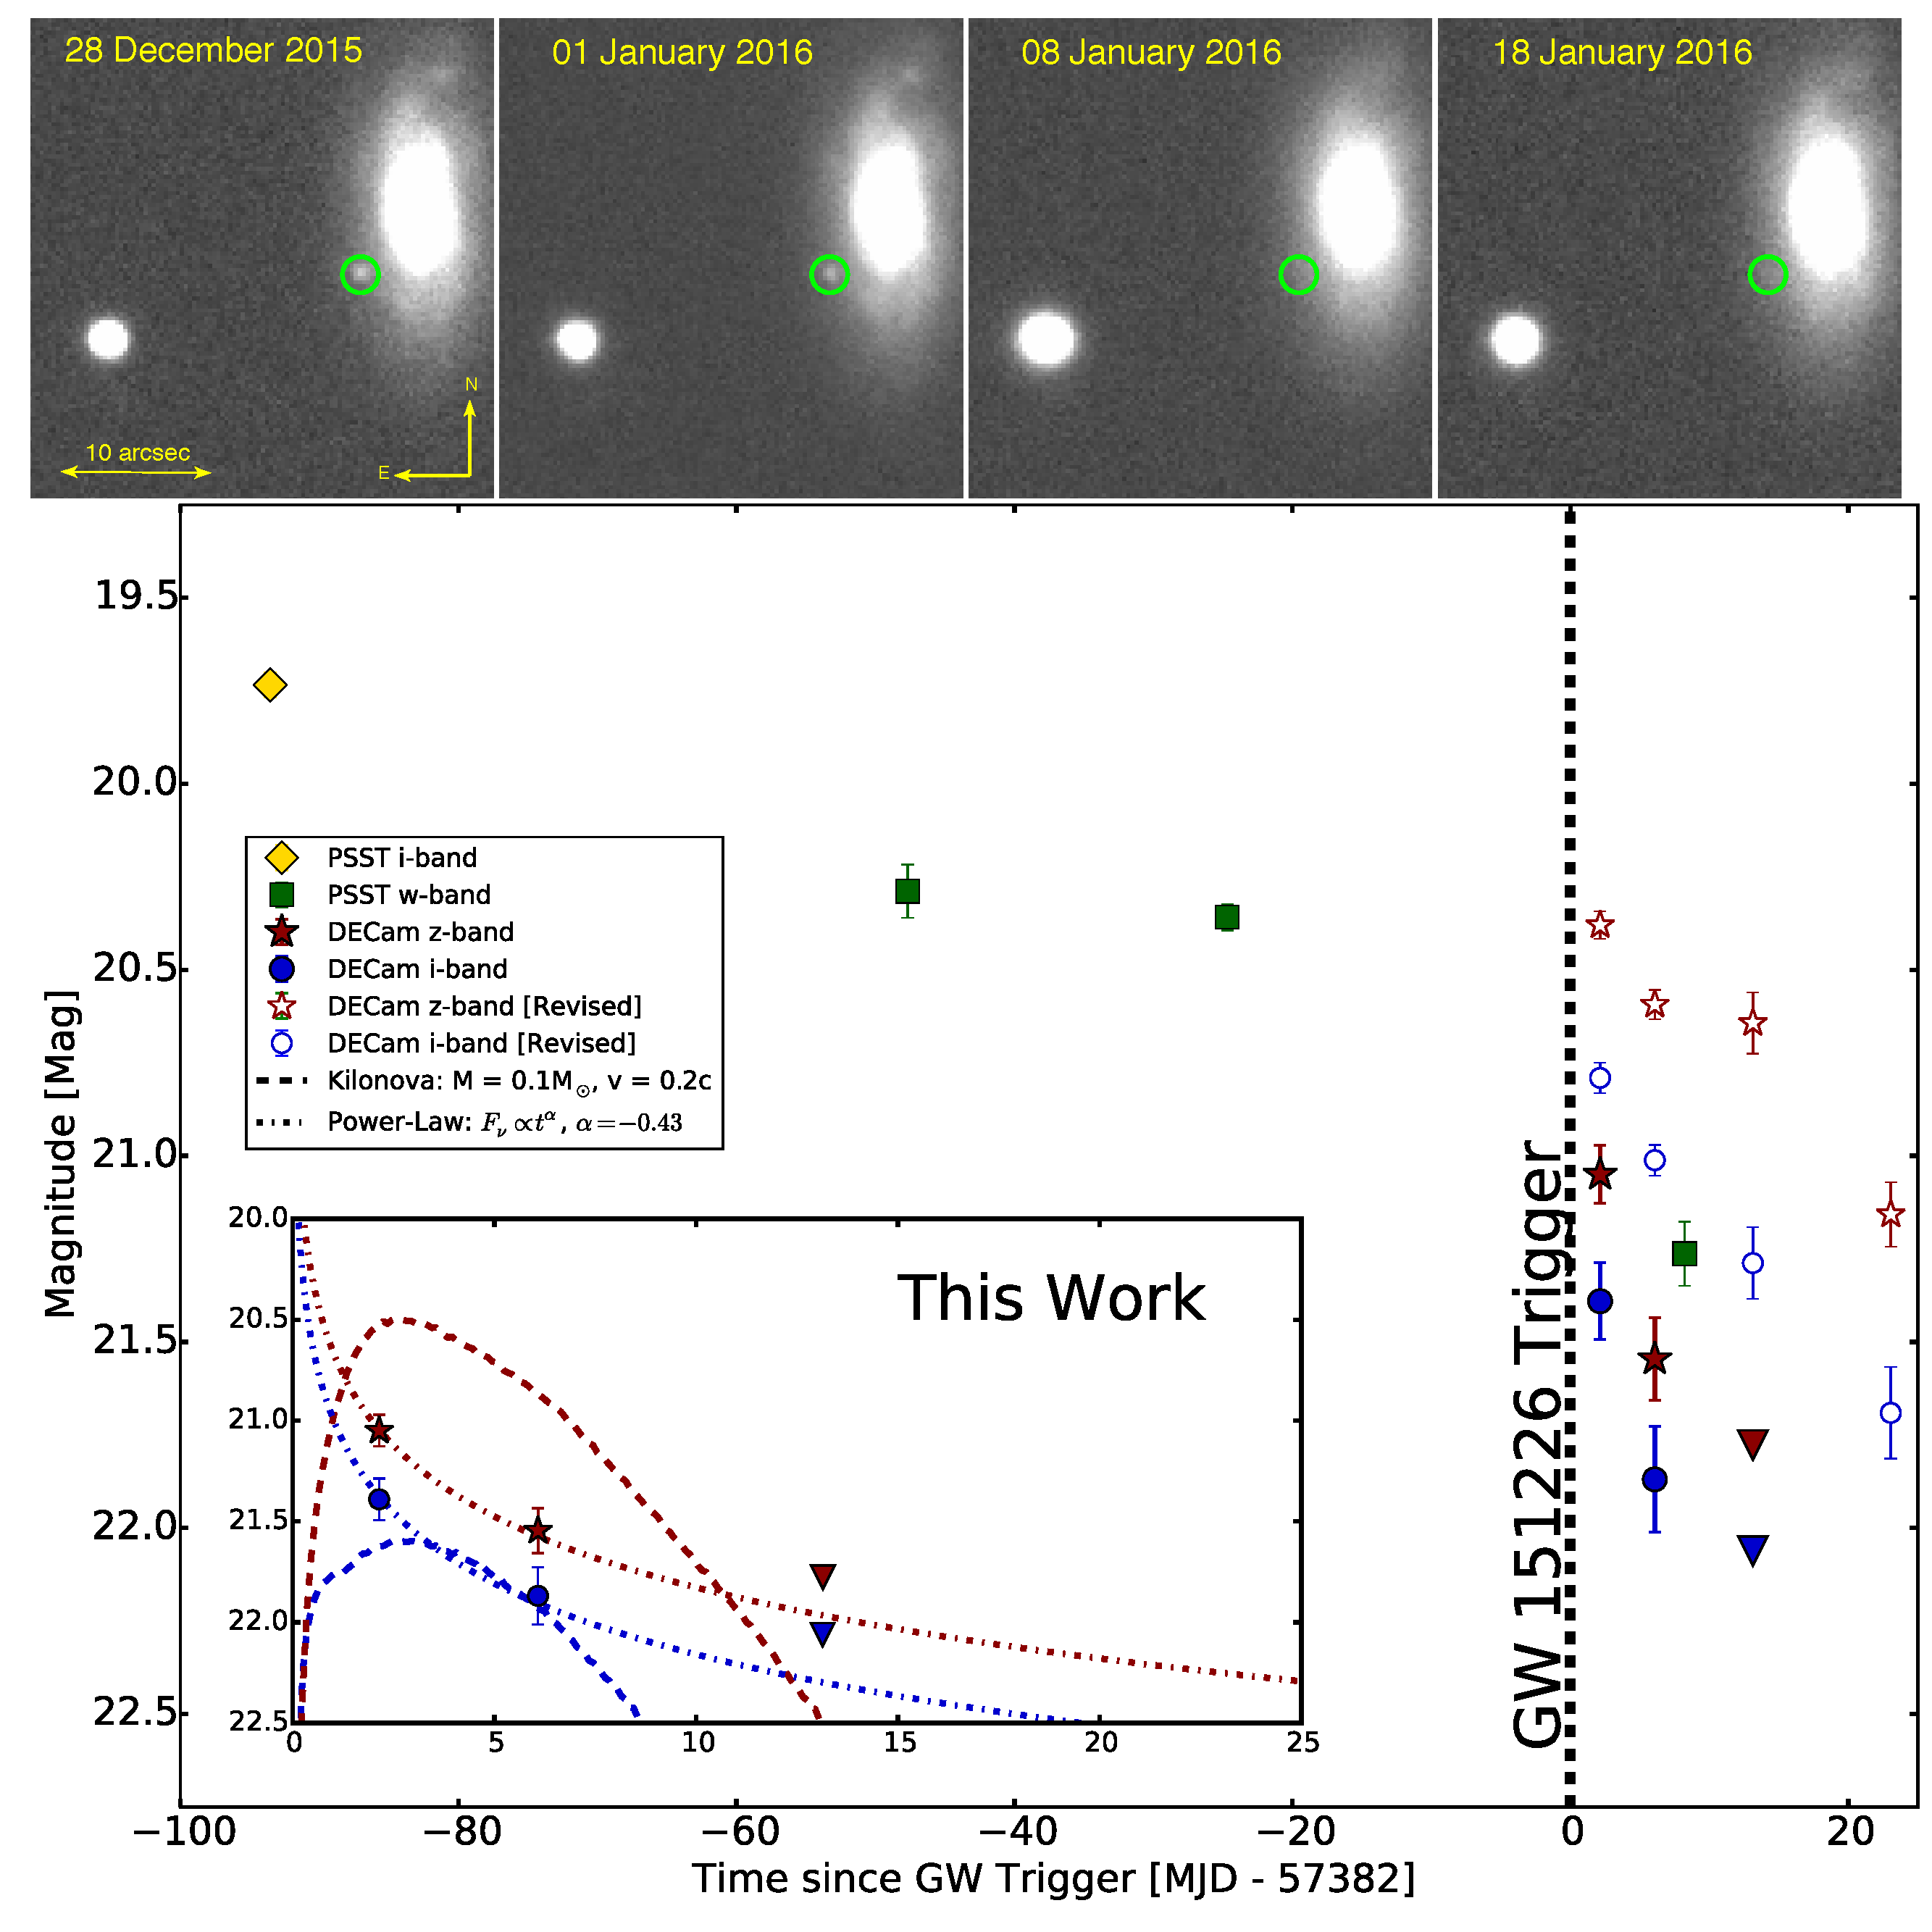
\includegraphics[width=0.9\textwidth]{./figs/chapter4/fig2.pdf}
 \caption{\singlespace {\it Top}: Single-epoch images of our main candidate
 from all four epochs (green circle). This is the event discovered as PS15cdi in
 the PSST about 94 d prior to GW151226. {\it Bottom}: Light
 curve data for PS15cdi from PSST $w$- and $i$-band
 observations (green squares and yellow diamonds, respectively).
 Our DECam $i$- and $z$-band data are shown as
 blue circles and red stars, respectively. The revised DECam analysis
 using pre-existing templates is shown as open symbols. Upper
 limits are indicated by triangles. The inset focuses on our
 DECam data, indicating a rapid decline in both $i$ and $z$
 bands.  We fit a power-law model to the data finding a temporal index of
 $\alpha = -0.43$ (dashed-dot line). Kilonova models from Barnes and
 Kasen \citeyearpar{BarnesKasen13} with $v_{\rm ej}=0.2c$ and $M_{\rm ej}=0.1$ M$_\odot$
 at a distance of $187$~Mpc are also shown (dashed line).}
 \label{fig:ch4_PS15cdi}
 \end{figure}

\clearpage
This source was previously detected as PS15cdi on 2015 September 23 by the Pan-STARRS
Survey for Transients (PSST\footnote{\singlespace \url{http://psweb.mp.qub.ac.uk/ps1threepi/psdb/candidate/1014216170021342600/}},
\citealt{Huber+15}); see \Cref{fig:ch4_PS15cdi}. The absolute $i$-band
magnitude in the first PSST epoch, $M_i\approx -16.6$ mag and the shallow decline of $\approx0.6$~mag
over $\approx70$~d, are consistent with a Type IIP core-collapse supernova (SN).
A likely interpretation of the rapid decline in our observations is that PS15cdi is a Type IIP SN undergoing
the rapid transition from the hydrogen recombination driven plateau to the radioactive $^{56}$Co dominated
phase \citep{KasenWoosley09,Sanders+15,Dhungana+16}. The red $i-z$ color in our data is consistent with observations
of other IIP SN during this phase of evolution (e.g., SN2013ej, \citealt{Dhungana+16}).
This transition typically occurs about 100~d post explosion \citep{KasenWoosley09,Sanders+15,Dhungana+16}, consistent with the
timing of our observations relative to the first detection in PSST.

To mitigate the effect of excess flux from PS15cdi still present in our template observations, we repeat the analysis
using as templates archival DES $i$- and $z$-band images from 2013 December 19. These data were processed
and image subtraction was performed as described in \cref{sec:ch4_obs}. We find that flux from PS15cdi is indeed still present
in our original template image, leading to revised first epoch absolute magnitudes of $M_i \approx -15.6$ and
$M_z \approx -16$~mag, and a decline rate between the first and fourth epochs of 0.04~mag d$^{-1}$, in both
$i$- and $z$-bands. The transient still exhibits a red $i-z$ colors of $\approx 0.4$~mag across all four epochs.

\clearpage
Clearly, we can rule out this candidate based on the PSST detections prior to
GW151226, but without this crucial information this candidate
would have been a credible optical counterpart based on its light curve behavior and distance.
It is therefore useful to develop an understanding of the expected rates for such contaminants
to inform expectations in future searches. We adopt a local core-collapse SN rate of
$7\times10^{-5}$~yr$^{-1}$~Mpc$^{-3}$ \citep{Li+11,Cappellaro+15},
and a Type IIP SN fraction of 48\% of this rate \citep{Smith+11}. The rapid
decline phase typically lasts about $20$~d \citep{KasenWoosley09,Sanders+15,Dhungana+16},
so we consider events that occur within that time frame. Lastly, given its apparent brightness,
we assume that PS15cdi represents the approximate maximum distance to which we can observe
these events in our data. We thus find an expected occurrence rate of $\sim 0.04$ events in our search area
making our detection of PS15cdi somewhat unlikely, and indicating that $\lesssim 1$ such
events are expected in a typical GW localization region.

Our detection of PS15cdi clearly demonstrates the presence and impact
of contaminants when conducting optical follow-up of GW events.
Core-collapse SNe are generally not considered to be a
significant contaminant due to their much longer timescales compared
to kilonovae (e.g., \citealt{CowpBerger15}). However, a
source like PS15cdi, caught in a rapid phase of its evolution
despite its overall long timescale, and
exhibiting a relatively red color could
satisfy a set of criteria designed for finding kilonovae ($\Delta m\gtrsim
0.1$ mag d$^{-1}$ and $i-z\gtrsim 0.3$ mag; \citealt{CowpBerger15}).

The most effective approach to deal with contaminants like PS15cdi is rapid,
real-time identification. Once a candidate is deemed interesting, optical spectroscopy and
NIR photometry can quickly distinguish between a SN or kilonova/afterglow
origin. If pre-existing templates are not available then the significant aspect is rapid initiation of
follow-up observations at $\lesssim 1$ d that can distinguish the rising phase of a kilonova or
off-axis GRB from a declining SN.

\section{Conclusions}
\label{sec:ch4_conc}
We presented the results of our deep optical follow-up of
GW151226 using the DECam wide-field
imager. Our observations cover a sky area of 28.8 deg$^2$,
corresponding to $3\%$ of the initial {\tt BAYESTAR} probability map
and 2\% of the final {\tt LALInference} map. We obtained
four epochs of observations starting 10 hours after the
event was announced and spanning 2--24 days post
trigger, with an average $5\sigma$ point-source sensitivity of
$i\approx21.7$ and $z\approx21.5$, with an epoch-to-epoch scatter
of 0.4 mag, in our difference images.

Using the final epoch as a template image, we searched for sources
that display a significant and steady decline in brightness
throughout our observations, and which are not present in the template
epoch. This search yielded four transients, of which three result from
 AGN variability. The final event is located at a distance of about
187 Mpc offset by $5.8''$ from its host galaxy. It also broadly possesses the
observational features of a kilonova in terms of its rapid decline and
red $i-z$ color. However, this source corresponds to the transient
PS15cdi, which was discovered in PSST about 94 days prior to the GW
trigger. It is a likely Type IIP supernova, which our observations
caught in the steep transition at the end of the plateau phase. The
detection of this event indicates that careful rejection of
contaminants, preferably in real time, is essential in order to avoid
mis-identifications of optical counterparts to GW sources.

%NOTE THE LACK OF A BIBLIOGRAPHY CALL IN THIS FILE. BIBLIOGRAPHY WORK HAPPENS OUTSIDE THE CHAPTER TEX FILES.

\clearpage
%
\chapter{Chapter 5 Title}\label{c:occ}
\chaptermark{Short Chapter 5 Title}
\begin{quote}
{\em ~~~~~~~This thesis chapter originally appeared in the literature as} \\
{authors,
{\em journal reference info}}
\end{quote}
%UNLIKE IN A REGULAR TEX FILE, DON'T PUT ANY PREAMBLE MATERIAL HERE

\section*{Abstract}
We present UV, optical, and NIR photometry of the first electromagnetic counterpart to a gravitational wave source from Advanced LIGO/Virgo, the binary neutron star merger GW170817. Our data set extends from the discovery of the optical counterpart at $0.47$ days to $18.5$ days post-merger, and includes observations with the Dark Energy Camera (DECam), Gemini-South/FLAMINGOS-2 (GS/F2), and the {\it Hubble Space Telescope} ({\it HST}). The spectral energy distribution (SED) inferred from this photometry at $0.6$ days is well described by a blackbody model with $T\approx 8300$ K, a radius of $R\approx 4.5\times 10^{14}$ cm (corresponding to an expansion velocity of $v\approx 0.3c$), and a bolometric luminosity of $L_{\rm bol}\approx 5\times10^{41}$ erg s$^{-1}$. At $1.5$ days we find a multi-component SED across the optical and NIR, and subsequently we observe rapid fading in the UV and blue optical bands and significant reddening of the optical/NIR colors. Modeling the entire data set we find that models with heating from radioactive decay of $^{56}$Ni, or those with only a single component of opacity from $r$-process elements, fail to capture the rapid optical decline and red optical/NIR colors. Instead, models with two components consistent with lanthanide-poor and lanthanide-rich ejecta provide a good fit to the data; the resulting ``blue'' component has $M_\mathrm{ej}^\mathrm{blue}\approx 0.01$ M$_\odot$ and $v_\mathrm{ej}^\mathrm{blue}\approx 0.3$c, and the ``red'' component has $M_\mathrm{ej}^\mathrm{red}\approx 0.04$ M$_\odot$ and $v_\mathrm{ej}^\mathrm{red}\approx 0.1$c. These ejecta masses are broadly consistent with the estimated $r$-process production rate required to explain the Milky Way $r$-process abundances, providing the first evidence that BNS mergers can be a dominant site of $r$-process enrichment.

\section{Introduction}
\label{sec:intro}
The era of gravitational wave (GW) astronomy began on 2015 September 14 when the Advanced Laser Interferometer Gravitational Wave Observatory (LIGO) made the first direct detection of gravitational waves, resulting from the merger of a stellar mass binary black hole (BBH; GW150914; \citealt{ligo1}). LIGO has since announced the detection of three additional BBH events \citep{ligo2,ligo3,ligo4}.  There are currently no robust theoretical predictions for electromagnetic (EM) emission associated with such mergers. 

By contrast, mergers involving at least one neutron star can produce a wide range of EM signals, spanning from gamma-rays to radio (e.g., \citealt{Metzger2012}). In the optical/NIR bands, the most promising counterpart is the kilonova (KN), a roughly isotropic thermal transient powered by the radioactive decay of rapid neutron capture ($r$-process) elements synthesized in the merger ejecta (\citealt{li1998,Metzger2010,Roberts2011,Metzger2012,Barnes2013,Tanaka2013}).    
The properties of the KN emission (luminosity, timescale, spectral peak) depend sensitively on the ejecta composition.  For ejecta containing Fe-group or light $r$-process nuclei with atomic mass number $A\lesssim 140$, the KN emission is expected to peak at optical wavelengths at a luminosity $L_{\rm p}\sim 10^{41}-10^{42}$ erg s$^{-1}$ on a short timescale of $t_{\rm p}\sim 1$ day (a so-called ``blue'' KN; \citealt{Metzger2010,Roberts2011,Metzger2014}).  By contrast, for ejecta containing heavier lanthanide elements ($A\gtrsim 140$) the emission is predicted to peak at NIR wavelengths with $L_{\rm p} \sim 10^{40}-10^{41}$ erg s$^{-1}$ over a longer timescale of $t_{\rm p}\sim 1$ week (a so-called ``red'' KN; \citealt{Barnes2013,Kasen2013,Tanaka2013}).

The first direct detection of gravitational waves from the inspiral and merger of a binary neutron star (BNS) was made on 2017 August 17 (GW170817; \citealt{ALVdetection,ALVSkymapgcn,ALVgcn}). This source was coincident with a short burst of Gamma-rays detected by both {\it Fermi}/GBM and {\it INTEGRAL} (GRB\,170817A; \citealt{GBMgcn1,GBMdetection,GBMgcn3,INTEGRALdetection,INTEGRALgcn,GBMgcn2}). Rapid optical follow-up by our DECam program \citep{DECamref}, starting just 11.4 hours after the GW trigger, led to the discovery of an associated optical counterpart in the nearby ($d\approx 39.5$ Mpc; \citealt{NGC4993dist}) galaxy NGC\,4993 \citep{DECAMgcn,DECampaper1}. This optical source was independently discovered by several groups \citep{GWEMcapstone}, and first announced as SSS17a by \cite{SWOPEpaper,SWOPEgcn}. The source has also been independently named DLT17ck \citep{DLT40paper,DLT40gcn}, and AT2017gfo.

Here we present rapid-cadence UV, optical, and NIR observations spanning from the time of discovery to 18.5 days post-merger.  We construct well-sampled light curves and SEDs using data from DECam along with {\it Swift}, GS/F2, and {\it HST}. We show that the data cannot be fit by a model with heating from $^{56}$Ni radioactive decay and Fe-peak opacities (as in normal supernovae), but instead requires heating from $r$-process nuclei and at least two components consistent with lanthanide-poor and lanthanide-rich opacities. We further use the data to determine the ejecta masses and velocities for each component.

All magnitudes presented in this work are given in the AB system and corrected for Galactic reddening with $E(B-V)=0.105$\footnote{This is computed from \url{http://irsa.ipac.caltech.edu/applications/DUST/} using the coordinate transients in \cite{DECampaper1}.} and applying the calibration of \cite{schlafly11}. We assume a negligible reddening contribution from the host \citep{DECamPaper8}. 

\begin{figure}[!t]
\begin{center}
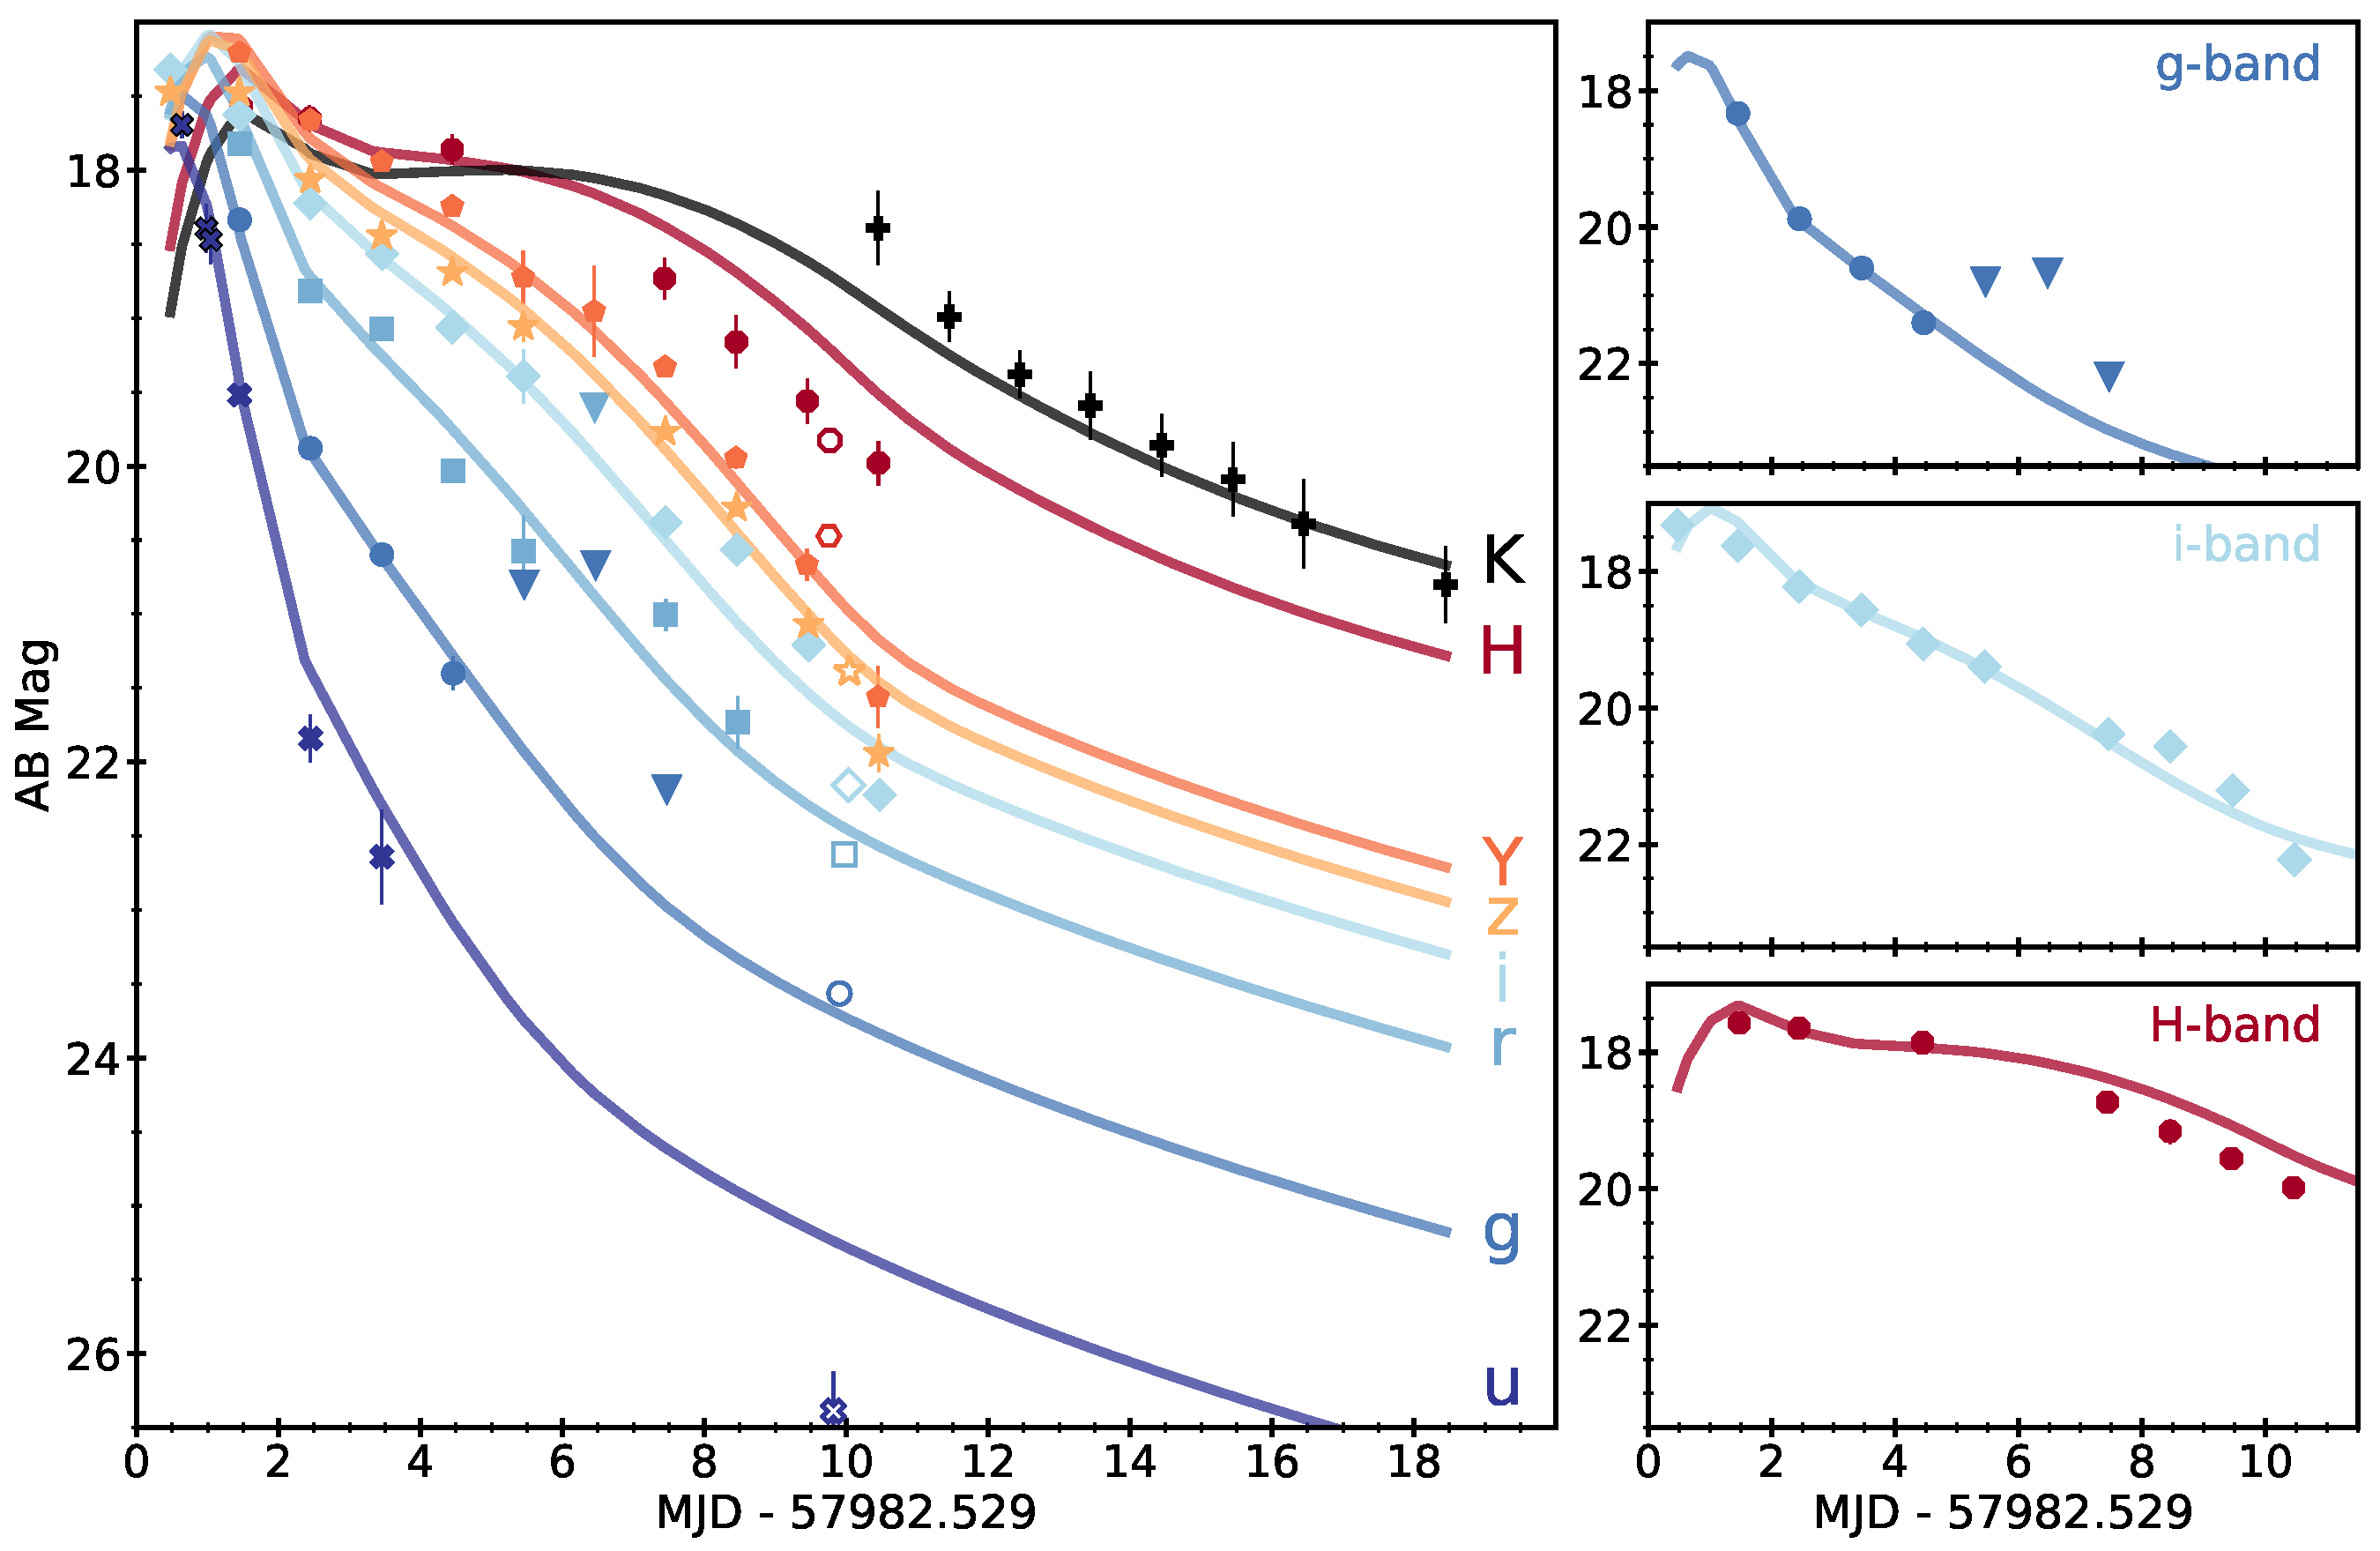
\includegraphics[width=0.9\textwidth]{./figs/chapter5/DECam_lc_alt.pdf}
\caption{UV, optical, and NIR Light curves of the counterpart of GW170817. The two-component model for $r$-process heating and opacities (\autoref{sec:models}) is shown as solid lines. The right panels focus on the $g$ (top), $i$ (middle), and $H$-band photometry (bottom), over the first 10 nights. Triangles represent 3$\sigma$ upper limits. Error bars are given at the $1\sigma$ level in all panels, but may be smaller than the points.}
\label{fig:lc_good}
\end{center}
\end{figure}

\section{Observations and Data Analysis}
\label{sec:observations}

A summary of the observations and photometry described in this section is available in \autoref{tab:phot}.

\subsection{DECam}
\label{sec:data}
We processed all DECam images using the {\tt photpipe} pipeline (e.g., \citealt{rest05,rest14}), to perform single-epoch image processing and image subtraction using the {\tt hotpants} software package \citep{becker15}. Point spread function (PSF) photometry was performed on the subtracted images using an implementation of {\tt DoPhot} optimized for difference images \citep{schechter93}. We performed astrometric and photometric calibration relative to the Pan-STARRS1/$3\pi$ catalog (PS1/$3\pi$; \citealt{PS1ref}), with appropriate corrections between magnitude systems \citep{scolnic15}. The typical calibration error is on the order of $\approx3\%$. Image subtraction was performed using stacked images from the PS1/$3\pi$ survey as reference images for $gr$-band. DECam images from 2017 August 25 and 2017 August 31 were used as reference images for $u$-band and $izY$-band, respectively, after the transient had faded away.

\subsection{HST}
\label{sec:data_HST} 
We obtained \textit{HST} Target-of-Opportunity observations of GW170817 on 2017 August 27.28 (9.8 days post-trigger) UT using ACS/WFC with the F475W, F625W, F775W, and F850LP filters, WFC3/UVIS with the F336W filter, and WFC3/IR with the F160W and F110W filters (PID: 15329; PI: Berger).  We retrieved the calibrated data from the Mikulski Archive for Space Telescopes (MAST) and used the {\tt DrizzlePac}\footnote{\url{http://drizzlepac.stsci.edu/}} software package to create final drizzled images from the individual dithered observations in each filter.  We used the {\tt astrodrizzle} task to correct for optical distortion and improve the resolution from that sampled by the instrumental PSF. We measure the flux of the optical counterpart by fitting a model PSF, constructed from multiple stars in each image, using a custom Python wrapper for {\tt DAOPhot} \citep{Stetson87}. We remove contaminating flux from the host galaxy at the transient location using local background subtraction. After subtraction, the typical contribution from the host flux is $\lesssim5\%$. We calibrate the photometry for each image using the zeropoints provided by the HST analysis team\footnote{\url{http://www.stsci.edu/hst/acs/analysis/zeropoints}}.

\subsection{GS/F2}
\label{sec:data_GSF2}
We obtained several epochs of $HK_s$ band photometry using FLAMINGOS-2 on the Gemini-South 8~m telescope \citep{GSF2ref2} starting on 2017 August 19.00 (1.47 days post-merger). We processed the images using standard procedures in the {\tt gemini} IRAF\footnote{IRAF is distributed by the National Optical Astronomy Observatory, which is operated by the Association of Universities for Research in Astronomy (AURA) under a cooperative agreement with the National Science Foundation.} package.  We created an average sky exposure from the individual dithered frames and then scaled and subtracted from each science image prior to registration and combination of the images. We perform PSF photometry using field stars and host galaxy subtraction as described in \autoref{sec:data_HST}, and calibrate the photometry relative to the 2MASS point source catalog \footnote{\url{https://www.ipac.caltech.edu/2mass/}}.

\subsection{Swift/UVOT}
\label{sec:data_UVOT}
The UVOT instrument on-board {\it Swift} \citep{Gehrels04, Roming05} began observing the field of the optical counterpart on 2017 August 18.167 UT with the {\it U}, {\it W1}, {\it W2}, and {\it M2} filters \citep{SWIFTgcn2,SWIFTgcn1,SWIFTpaper}.  We use the latest {\tt HEAsoft} release (v6.22) with the corresponding calibration files and updated zero-points to independently analyze the data. We perform photometry in a $3\arcsec$ photometric aperture to minimize the contamination from host galaxy light, following the prescriptions by \citet{Brown09}. We estimate and subtract the contribution from host galaxy light using deep UVOT observations acquired at later times, when the UV emission from the transient was no longer present in the images ({\it Swift} ID 07012979003). The systematic effect from the host light contamination is $\approx 3\%$ (see e.g., \citealt{Brown09}).

\section{Light Curves and Spectral Energy Distributions}
\label{sec:analysis}

\begin{figure}[!t]
\begin{center}
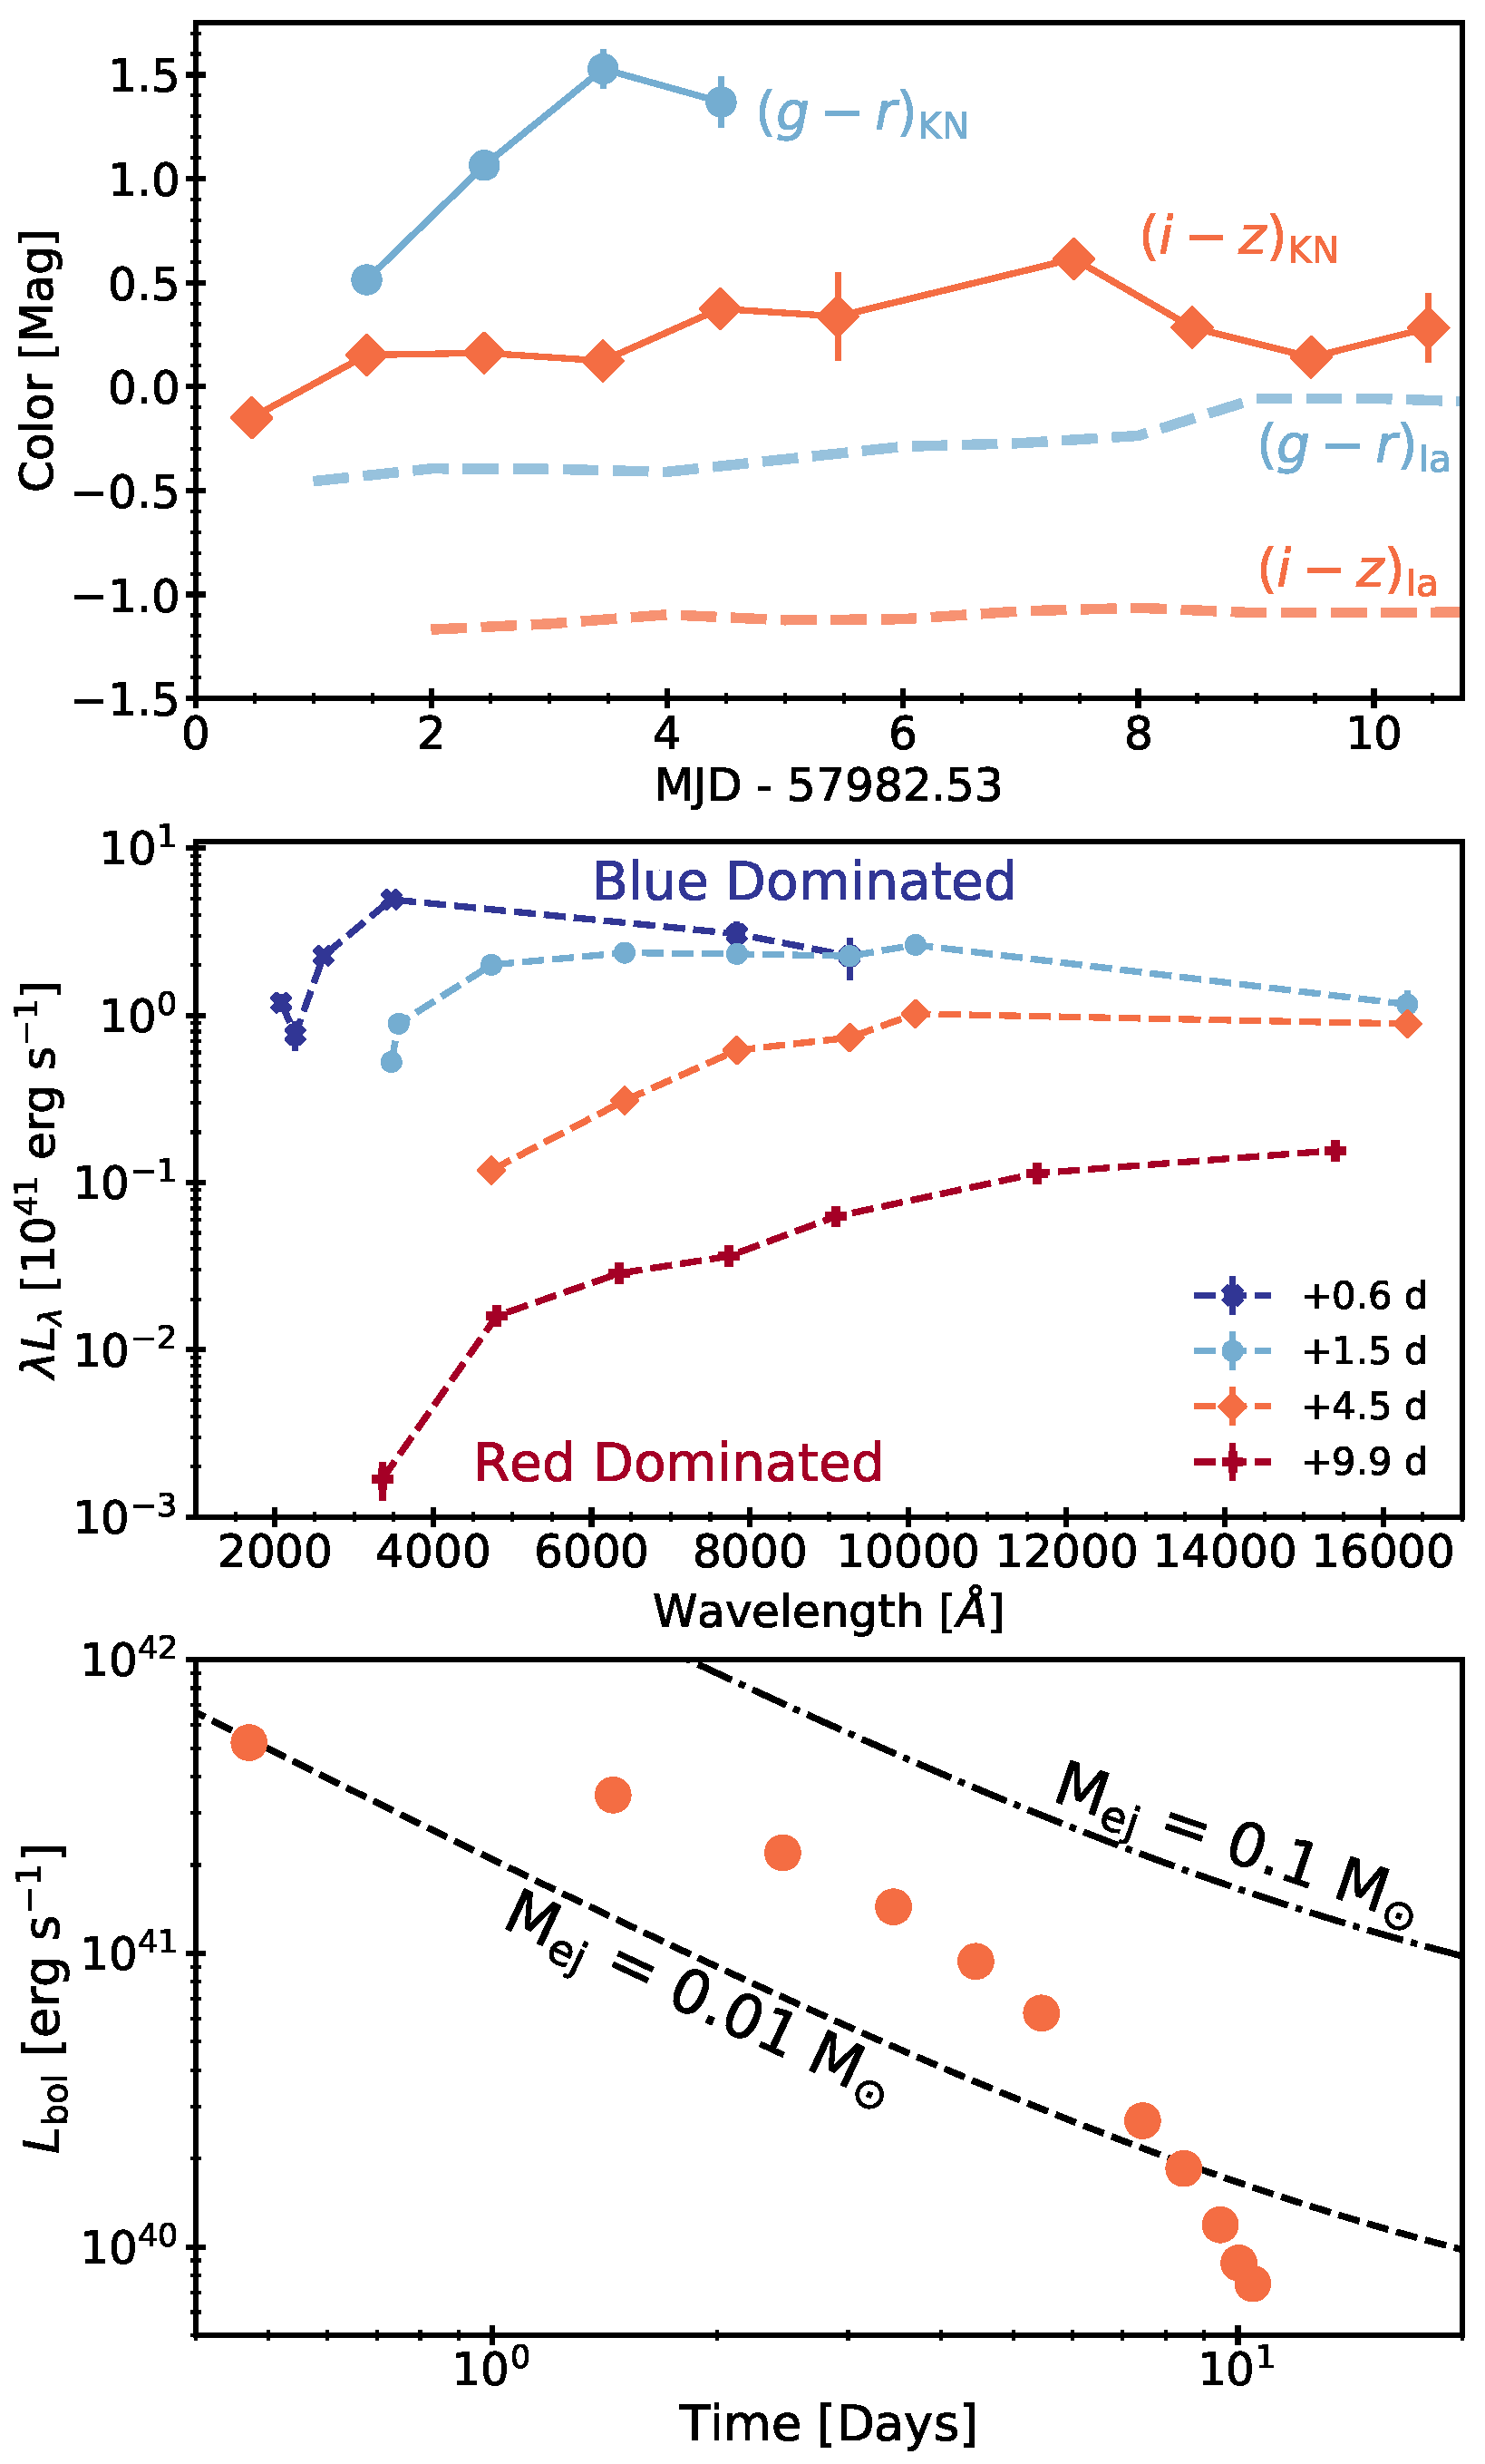
\includegraphics[width=0.575\textwidth]{./figs/chapter5/sed_col_bol_alt.pdf}
\caption{{\it Top:} Optical colors from DECam observations as a function of time.  We observed rapid and early reddening in $g-r$ compared to the relatively flat but red $i-z$ colors. Also shown are template Ia SN colors relative to explosion for comparison \citep{nugent2002k}. {\it Middle:} SEDs at four representative epochs (assuming isotropic emission). The transition from a blue dominated spectrum at early times to a spectrum dominated by a red component at late times is clearly visible. {\it Bottom:} Bolometric light curve spanning $ugrizYH$. Expected values for $r$-process heating from \cite{Metzger2010} are shown for comparison, indicating that the observed emission requires ${\rm few}\times 10^{-2}$ M$_\odot$ of $r$-process ejecta. Error bars are given at the $1\sigma$ level in all panels, but may be smaller than the points.}
\label{fig:sed}
\end{center}
\end{figure}

\subsection{Light Curves}
\label{sec:lc}

Our UV/optical/NIR light curves are shown in \autoref{fig:lc_good}. The data span from 0.47 to 18.5 days post merger, with bluer bands fading below the detection limits at earlier times.  The light curve coverage was truncated by the proximity of the source to the Sun.  We first note that the light curves are not well described by a power law, indicating minimal contribution from a GRB optical afterglow over the timescale of our observations. This is consistent with modeling of the afterglow based on X-ray and radio observations \citep{DECamPaper6,DECamPaper5}.

The light curves exhibit a rapid decline in the bluest bands ($ug$), an intermediate decline rate in the red optical bands ($rizY$), and a shallow decline in the NIR ($HK_s$).  However, while the $u$- and $g$-band light curves decline by $\approx 2$ mag d$^{-1}$ starting with the earliest observations, the redder optical bands exhibit a more complex behavior: they exhibit a comparatively slow decline ($\approx0.3$ mag d$^{-1}$) over the first 1.5 days, develop a shoulder at about 4 days, and subsequently begin to decline at about 8 days.

We find a similar rapid evolution in the colors of the transient (\autoref{fig:sed}).  In particular, the $u-g$ and $g-r$ colors become redder by about 1 mag between about 1.5 and 3.5 days.  The colors in the redder optical bands exhibit slower evolution, with $r-i\approx 0.5-1$ mag, $i-z\approx 0-0.5$ mag, and $z-Y\approx 0.3$ mag.  These colors are significantly redder than those of known supernovae near explosion (e.g., \citealt{folatelli2009,bianco2014,galbany2016}).

\subsection{Spectral Energy Distribution}
\label{sec:SED}

We construct SEDs from photometry at several epochs from about 0.6 to 10 days post-merger (\autoref{fig:sed}). The SEDs exhibit rapid evolution from an initial peak at \apx3500 $\mbox{\AA}$ to a final peak at $\gtrsim 15,000$~$\mbox{\AA}$ by 10 days.  Moreover, the SED at 1.5 days appears to consist of two components, as indicated by the changing slope in the NIR emission. The same rapid evolution and structure are apparent in the optical and NIR spectra at comparable epochs \citep{DECamPaper4,DECamPaper3}.

The SED at 0.6 days is well described by a blackbody with $T\apx 8300$ K and $R\apx 4.5\times 10^{14}$ cm, corresponding to an expansion velocity of $v\apx 0.3c$. This is somewhat larger than the velocities observed in broad-lined Type Ic SNe (for which $v\approx 0.1c$; \citealt{modjaz2016}), but is consistent with expectations for ejecta resulting from a BNS merger \citep{Metzger2017}. The SEDs at later times are not well described by a blackbody curve, instead exhibiting strong flux suppression at blue wavelengths that leads to a spectrum with a sharper peak than a blackbody.  This behavior is also present in our optical spectra \citep{DECamPaper3}.

\subsection{Bolometric Light Curve}
\label{sec:lc_bol}

We construct a bolometric light curve from the $ugrizYH$ data spanning to 11 days. We fit the time evolution in each band independently with a linear model and interpolate the magnitudes to a common grid of times. The bolometric luminosity is determined using the integrated total flux at each time step; see \autoref{fig:sed}. The peak bolometric luminosity of $\apx5\times10^{41}$ ergs s$^{-1}$ at 0.6 days is broadly consistent with the luminosity predicted for $r$-process heating by a ${\rm few}\times 10^{-2}$ M$_{\odot}$ ejecta, similar to the original predictions of \cite{Metzger2010} for blue KN emission from Fe-opacity ejecta. The total radiated energy during the first \apx10 days is $\approx10^{47}$~ergs.

\subsection{Qualitative Comparisons to Kilonova Emission}
\label{sec:kn_compare}
There are several lines of preliminary evidence that suggest the optical counterpart is an $r$-process powered kilonova before exploring detailed models. The presence of an initially blue SED, transitioning to a multi-component SED, and finally to a red SED, is strongly suggestive of both blue and red kilonova emission, consistent with  lanthanide-poor and rich ejecta components, respectively \citep{Metzger2010,Barnes2013,Tanaka2013,Metzger2014,kasen15,Wollaeger2017}. Furthermore, the deviations from a pure blackbody spectrum at late times are indicative of the strong UV line blanketing expected for lanthanide-rich material, lending further evidence to the existence of a red kilonova component. This behavior is also seen in optical/NIR spectra of the transient \citep{DECamPaper4,DECamPaper3}.

The fact that this red component does not initially obscure the emission from a blue component suggests that we require two separate emitting regions with distinct sources of ejecta. If the KN outflow is quasi-spherical, then the blue component must reside {\it outside} the material with red emission.  Alternatively, if the outflow is not spherically symmetric, the blue and red ejecta should occupy distinct portions of the outflowing solid angle. This feature is suggested in several models that consider lanthanide-rich material ejected in the equatorial plane while the lanthanide-poor material is ejected from the polar regions \citep{kasen15,Metzger2017}. 

\begin{deluxetable}{cccccccccccc}
\tabletypesize{\footnotesize}
\tablecolumns{12}
\tablewidth{0pt}
\tablecaption{Kilonova Model Fits
	          \label{tab:KN}}
\tablehead{
\colhead{Model} & 
\colhead{$M_{\rm ej}^{\rm blue}$} & 
\colhead{$v_{\rm ej}^{\rm blue}$} &
\colhead{$\kappa^{\rm blue}$} &
\colhead{$M_{\rm ej}^{\rm purple}$} & 
\colhead{$v_{\rm ej}^{\rm purple}$} &
\colhead{$\kappa^{\rm purple}$} &
\colhead{$M_{\rm ej}^{\rm red}$} & 
\colhead{$v_{\rm ej}^{\rm red}$} &
\colhead{$\kappa^{\rm red}$} &
\colhead{$f^{\rm Ni}$} &
\colhead{WAIC} \\
\colhead{} & 
\colhead{($\text{M}_{\odot}$)} & 
\colhead{(c)} & 
\colhead{($\text{cm}^2 \text{g}^{-1}$)} & 
\colhead{($\text{M}_{\odot}$)} & 
\colhead{(c)} & 
\colhead{($\text{cm}^2 \text{g}^{-1}$)} & 
\colhead{($\text{M}_{\odot}$)} & 
\colhead{(c)} & 
\colhead{($\text{cm}^2 \text{g}^{-1}$)} & 
\colhead{}&
\colhead{}
}
\startdata
2-Comp & $0.014^{+0.002}_{-0.001}$ & $0.266^{+0.007}_{-0.002}$ & (0.5) & - & - & - & $0.036^{+0.001}_{-0.002}$ & $0.123^{+0.012}_{-0.014}$ & $3.349^{+0.364}_{-0.337}$  & - & -102 \\
3-Comp & $0.014^{+0.002}_{-0.001}$ & $0.267^{+0.006}_{-0.011}$ & (0.5) & $0.034^{+0.002}_{-0.002}$ & $0.110^{+0.011}_{-0.010}$ & (3.0) & $0.010^{+0.002}_{-0.001}$ & $0.160^{+0.030}_{-0.025}$ & (10.0) & - &  -106 \\
\hline
$^{56}$Ni & $0.008^{+0.007}_{-0.001}$ & $0.260^{+0.034}_{-0.031}$ & (0.1) & - & - & - & - & - & -  & $0.749^{+0.214}_{-0.203}$ & 17\\
Blue & $0.032^{+0.002}_{-0.004}$ & $0.180^{+0.002}_{-0.002}$ & (0.1) & - & - & - & - & - & -  & - & 17\\
Red & - & - & - & - & - & - & $0.026^{+0.010}_{-0.008}$ & $0.271^{+0.008}_{-0.002}$ & (10) & - & 153\\
1-Comp & - & - & - & $0.040^{+0.002}_{-0.007}$ & $0.274^{+0.007}_{-0.093}$ & $0.817^{+0.146}_{-0.135}$  & - & - & - & - &  11
\enddata
\tablecomments{Model parameters and WAIC scores. Numbers in parentheses indicate fixed parameters of the model. The errors represent the 1$\sigma$ confidence interval. Both the 2-component (``2-Comp'') and 3-component (``3-Comp'') models have significantly smaller WAIC scores (indicating better fits) compared to the four single-component models. }
\end{deluxetable}

\section{Kilonova Modeling}
\label{sec:models}

We test the conjecture that the UV/optical/NIR transient is an $r$-process kilonova by fitting several isotropic, one-zone, gray opacity models to the light curves. For each model, we assume a blackbody SED which evolves assuming a constant ejecta velocity until it has reached a minimum temperature, at which point the photosphere has receded into the ejecta and the temperature no longer evolves. A similar temperature ``floor'' is predicted in \cite{Barnes2013}, and we include this minimum temperature as a fitted parameter.  We additionally fit for a ``scatter'' term, added in quadrature to all photometric errors, which roughly accounts for additional systematic uncertainties that are not included in our model. 

We use {\tt MOSFiT}\footnote{\url{https://github.com/guillochon/MOSFiT}} \citep{mosfitpaper,nicholl2017magnetar}, an open source light curve fitting tool that utilizes a Markov Chain Monte Carlo (MCMC) to sample the model posterior. For each model, we ensure convergence by enforcing a Gelman-Rubin statistic $<1.1$ \citep{gelman1992inference}.  We compare models using the Watanabe-Akaike Information Criteria (WAIC, \citealt{watanabe2010asymptotic,gelman2014understanding}), which accounts for both the likelihood score and number of fitted parameters. The best fit parameters, uncertainties, and WAIC scores for each model are provided in Table~\ref{tab:KN}.

We first attempt a simple supernova model, namely heating by the radioactive decay of $^{56}$Ni and Fe-peak opacity of $\kappa = 0.1$ cm$^{2}$ g$^{-1}$ (see \citealt{villar2017}).  The model parameters are the ejecta mass and velocity, and the $^{56}$Ni mass fraction in the ejecta (as well as the temperature floor and scatter).  The best-fit model has $M_{\rm ej}\approx 0.01$ M$_\odot$, $v_{\rm ej}\approx 0.26$c, and $f^{\rm Ni}\approx 0.75$.  The parameters are comparable to those we inferred from black body fits to the flux and SEDs in the previous section, but the overall fit is poor.  In particular, this model severely underestimates the NIR light curves, while the high $^{56}$Ni fraction is inconsistent with the optical spectra \citep{DECamPaper3}.  We therefore conclude that the transient is not powered by the radioactive decay of $^{56}$Ni.

\begin{figure}
\begin{center}
\hspace*{-0.1in} 
\scalebox{1.}
{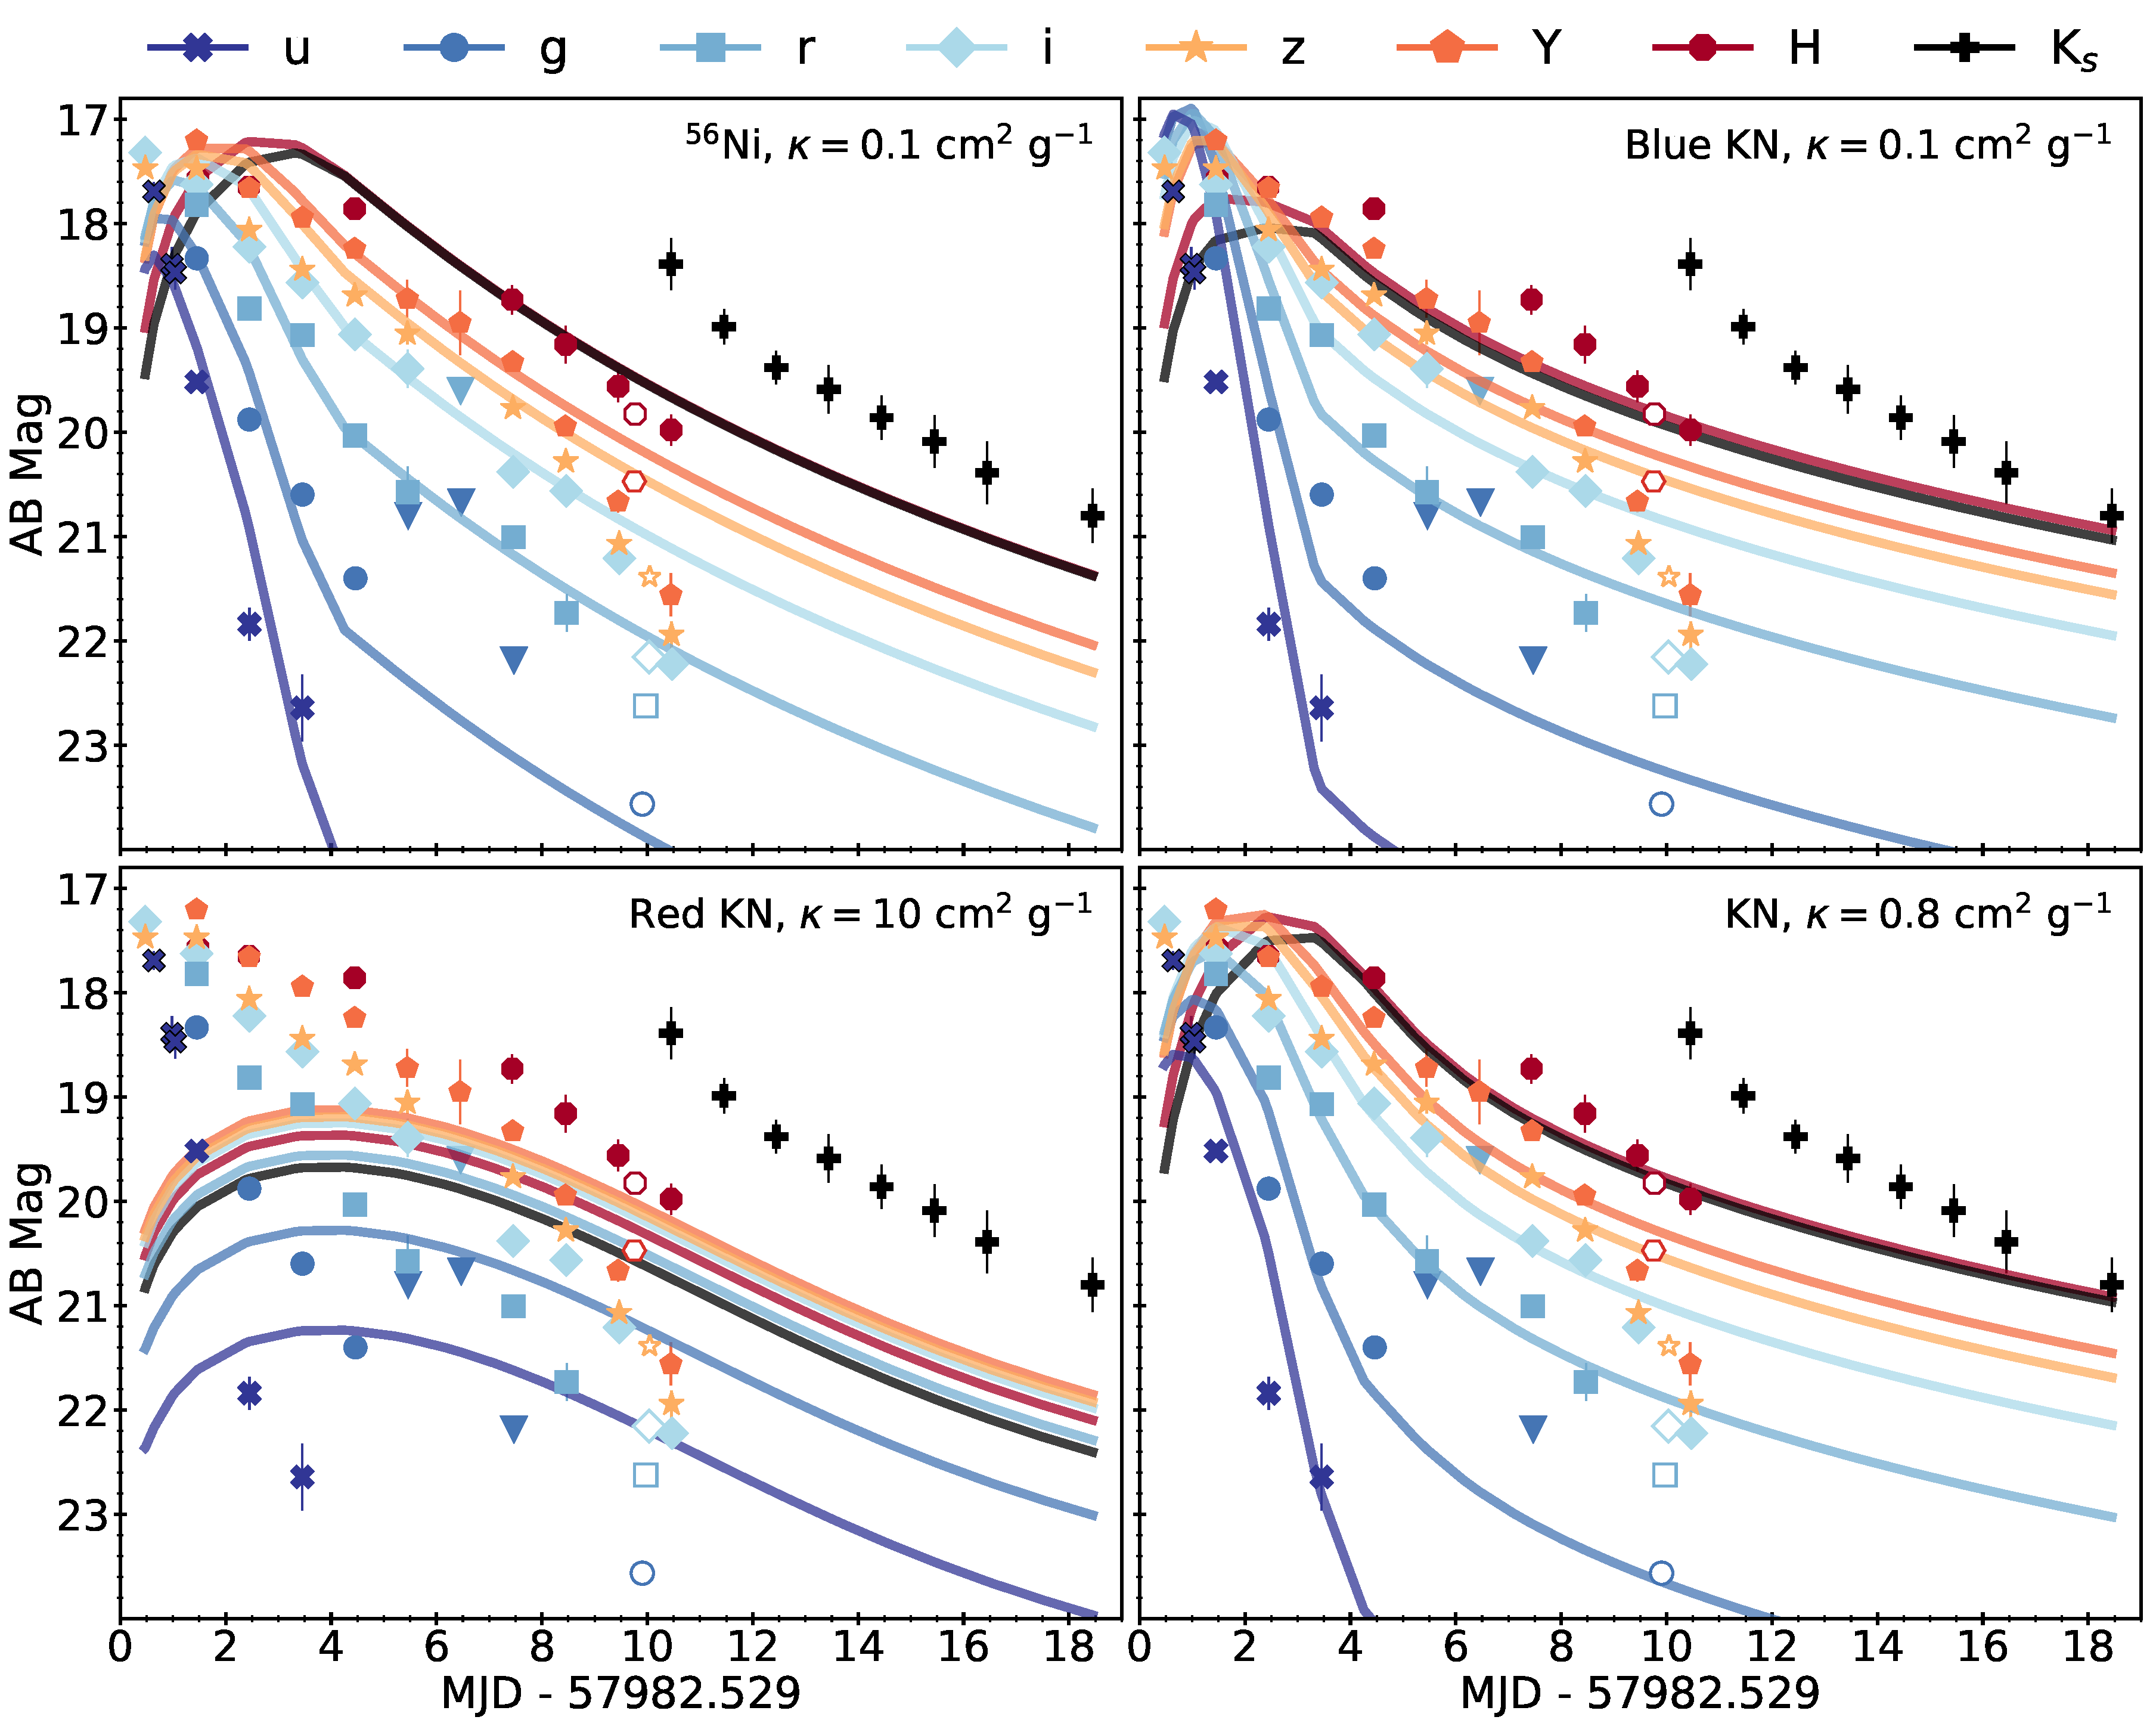
\includegraphics[width=0.9\textwidth]{./figs/chapter5/lc_failed_alt.pdf}}
\caption{{\it Top Left:} Fitting the data with a Type I b/c SN model powered by the radioactive decay of $^{56}$Ni. This model clearly fails to capture the late time NIR behavior and requires an unphysically large fraction of the ejecta to be synthesized into nickel (\apx75\%). {\it Top Right:} Fitting the data with a single component ``blue'' KN model. Like the SN model, this fit is unable to capture the late time NIR behavior and overall spectra shape. {\it Bottom Left:} Fitting the data with a single component ``red'' KN model. This model clearly fails to capture any of the observed behavior. {\it Bottom Right:} Fitting the data with a single-component KN model with the opacity as a free parameter. Again, this model fails to capture the late time NIR behavior. This is suggestive of the fact that we need to model multiple ejecta components simultaneously. Error bars are given at the $1\sigma$ level in all panels, but may be smaller than the points.}
\label{fig:lc_failed}
\end{center}
\end{figure}

We next turn to $r$-process heating, using the model outlined in \citet{Metzger2017} and implemented in \citet{villar2017}. This model includes the ejecta mass, ejecta velocity and opacity as fitted parameters (as well as the temperature floor and scatter). Within this context we first assume an Fe-peak opacity of $\kappa = 0.1$ cm$^{2}$ g$^{-1}$ (our "blue" model; e.g., as assumed historically in \citealt{li1998}) and fit for the ejecta mass and velocity.  This model, with $M_{\rm ej}\approx 0.03$ M$_\odot$ and $v_{\rm ej}\approx 0.18$c, adequately describes the early light curves ($\lesssim 3$ d), but again is a poor fit to the NIR light curves.  More recent calculations indicate that lanthanide-rich ejecta are expected to have a much higher opacity of $\kappa = 10$ cm$^{2}$ g$^{-1}$, leading to a ``red'' kilonova (e.g., \citealt{Barnes2013}).  However, such a model (our ``red" model), with best fit values $M_{\rm ej}\approx 0.03$ M$_\odot$ and $v_{\rm ej}\approx 0.27$c, produces a poor fit to the data as well.  In particular, the model light curves exhibit an initial rise for $\approx 4$ days, in contrast to the observed rapid decline at early time, especially in the UV and blue optical bands.  Finally, we allow the opacity to vary as a free parameter, finding a best fit value of $\kappa \approx 0.82$ cm$^{2}$ g$^{-1}$, and an associated $M_{\rm ej}\approx 0.04$ M$_\odot$ and $v_{\rm ej}\approx 0.27$c.  However, this model again fails to reproduce the initial rapid decline in the UV, as well as the NIR light curves.  We therefore conclude that $r$-process heating with a single value for the opacity cannot explain the observed light curve evolution and colors. The final light curves for these models can be seen in \autoref{fig:lc_failed}.

Inspired by the multi-component observed SED (Figure~\ref{fig:sed}) and by the failure of single-component models to capture both the early rapid decline and the late-time red colors, we explore two multi-component models: (i) a two-component ``blue'' ($\kappa = 0.5$ cm$^{2}$ g$^{-1}$) plus ``red'' ($\kappa$ as a free parameter) model; and (ii) a three-component ``blue'' ($\kappa = 0.5$ cm$^{2}$ g$^{-1}$) plus ``purple'' ($\kappa = 3$ cm$^{2}$ g$^{-1}$) plus ``red'' ($\kappa = 10$ cm$^{2}$ g$^{-1}$) model. These values were recently shown by \citet{Tanaka2017} to roughly capture the detailed opacity from radiative transfer simulations. For each component we leave $M_{\rm ej}$ and $v_{\rm ej}$ as free parameters.

First, we explore the two-component model (with eight free parameters); we vary the ejecta masses, ejecta velocities, and temperature floors, the red component opacity, and a single scatter term. We find that the ``blue'' component has $M_\mathrm{ej}^\mathrm{blue}\approx 0.01$ M$_\odot$ and $v_\mathrm{ej}^\mathrm{blue}\approx 0.27$c (with errors of roughly 10\%), in good agreement with our inference from the SED at early time (\autoref{sec:SED}). The ``red'' component has a much larger mass of $M_\mathrm{ej}^\mathrm{red}\approx 0.04$ M$_\odot$ but a slower velocity of $v_\mathrm{ej}^\mathrm{red}\approx 0.12$c. The best-fit opacity of this component is $\kappa\approx 3.3$ cm$^{2}$ g$^{-1}$, lower than expected for lanthanide-rich ejecta. We find that most of the parameters are uncorrelated, with the exception of the red component's opacity and ejecta velocity, which have a Pearson correlation coefficient of $\sim0.67$. The resulting parameters and uncertainties from the MCMC fitting are summarized in Table~\ref{tab:KN}.

For the three-component model (with ten free parameters) we find similar values for the ``blue'' component ($M_\mathrm{ej}^\mathrm{blue}\approx 0.01$ M$_\odot$ and $v_\mathrm{ej}^\mathrm{blue}\approx 0.27$c) and the ``purple'' component ($M_\mathrm{ej}^\mathrm{purple}\approx 0.03$ M$_\odot$ and $v_\mathrm{ej}^\mathrm{purple}\approx 0.11$c).  The ``red'' component is sub-dominant with $M_\mathrm{ej}^\mathrm{red}\approx 0.01$ M$_\odot$ and $v_\mathrm{ej}^\mathrm{red}\approx 0.16$c); see Table~\ref{tab:KN}. These ejecta parameters are consistent with those determined from independent modeling of the optical and NIR spectra \citep{DECamPaper4,DECamPaper3}.

Both sets of models are shown in Figure~\ref{fig:lc_good} and are essentially indistinguishable.  Both provide a much better fit to the data than the single-component models described above, capturing both the initial blue colors and rapid decline, as well as the later redder colors and NIR light curves.  Their similar WAIC scores suggest that neither model is statistically preferred. The two models differ most drastically at $\lesssim 5$ days in the $K_s$-band, where the two-component model is double-peaked, while the three-component model is single peaked. While neither model fully captures every feature of the light curves, it is remarkable that these simplified semi-analytic models produce such high quality fits over a wide range of wavelength and time. 

\section{Implications}
\label{sec:interpretation}

In the multi-component models, we can interpret each component as arising from distinct physical regions within the merger ejecta. In both models, the high velocity of the blue KN ejecta suggests that it originates from the shock-heated polar region created when the neutron stars collide (e.g.~\citealt{Oechslin2007,Bauswein2013,Sekiguchi2016}). This dominant blue component is also seen in early time optical spectra \citep{DECamPaper3}. By contrast, the low velocity red KN component in our three-component model could originate from the dynamically-ejected tidal tails in the equatorial plane of the binary (e.g., \citealt{Rosswog1999,Hotokezaka2013}), in which case the relatively high ejecta mass $\approx 0.01$ M$_{\odot}$ suggests an asymmetric mass ratio of the merging binary (q$\lesssim0.8$; \citealt{Hotokezaka2013}).

In both multi-component models we find that the $\kappa\approx 3$ cm$^{2}$ g$^{-1}$ ejecta dominates by mass.  The lower velocity of this component suggests an origin in the post-merger accretion disk outflow.  Our inferred ejecta mass is consistent with that expected for a massive $\sim 0.1$ M$_{\odot}$ torus (e.g., \citealt{Just2015,Siegel&Metzger2017}).  Similarly, the disk outflow composition is predicted to be dominated by $Y_{e}\sim 0.3$ matter that produces the $\kappa\approx 3$ cm$^{2}$ g$^{-1}$ component of the KN emission \citep{Tanaka2017} as we observe. The fitted opacity indicates that the hyper-massive neutron star remnant is relatively short-lived ($\sim 30$ ms; \citealt{Fernandez2013,Just2015,kasen15}). We additionally find that in both models the total kinetic energy is roughly $(1-2)\times 10^{51}$ erg.

The fact that our multi-component models fit the data well provides strong evidence for the production of both light and heavy $r$-process nuclei, addressing one of the long-standing mysteries in astrophysics \citep{Burbidge1957,Cameron1957}. We quantify this statement by comparing our blue and red ejecta masses to those necessary to reproduce the Milky Way $r$-process production rate.  For heavy $r$-process elements (red KN), the Milky Way inferred production rate is $\dot{M}_\mathrm{rp,A\gtrsim 140}\approx 10^{-7}$ M$_\odot$ yr$^{-1}$ \citep{bauswein2014nucleosynthesis}. For light $r$-process elements (blue KN), the production rate is $\dot{M}_\mathrm{rp,A\gtrsim 100}\approx 7\times 10^{-7}$ M$_\odot$ yr$^{-1}$ \citep{qian2000supernovae}. Using a conservative estimate on the local BNS merger rate estimated by \citet{abbott2016upper}, $R_\mathrm{0}\approx 1000$ Gpc$^{-3}$ yr$^{-1}$, and a volume density of Milky Way-like galaxies of $\approx 0.01$ Mpc$^{-3}$, we estimate the Milky Way rate of KN as $R_\mathrm{MW}\approx 100$ Myr$^{-1}$.  Using this MW rate, we find that the average ejecta mass for a red KN is $\dot{M}_\mathrm{rp,A\gtrsim 140}/R_\mathrm{MW}\approx 0.001$ M$_\odot$ and for a blue KN it is $\dot{M}_\mathrm{rp,A\gtrsim 100}/R_\mathrm{MW}\approx 0.007$ M$_\odot$. These order-of-magnitude estimates are  smaller than our inferred ejecta masses for this event, although the discrepancy can potentially be mitigated when properly taking into account the fraction of $r$-process materials which remains in a gas phase in the ISM and galactic halo. Nevertheless, this exercise suggests that BNS mergers can reproduce the $r$-process yields found in the Milky Way and may be a dominant source of cosmic $r$-process nucleosynthesis.

\section{Discussions and Conclusions}
\label{sec:conc}

We presented a comprehensive UV, optical, and NIR data set for the first electromagnetic counterpart to be associated with a gravitational wave event.  Analysis of these data reveal that the emission is due to an $r$-process powered kilonova consisting of both ``blue'' and ``purple/red'' ejecta components. Models with $^{56}$Ni heating, Fe-peak opacities, or a single component of $r$-process opacity fail to match the observations.

Our models indicate that the total ejecta mass is $\approx 0.05$ M$_\odot$, with a high velocity ($v\approx 0.3c$) blue component and a slower ($v\approx 0.1-0.2c$) purple/red component.  The presence of both components and the relatively large ejecta mass suggests that binary neutron star mergers (like GW170817) dominate the cosmic $r$-process nucleosynthesis.

The data presented in this paper (and others in this series) represent by far the best observations of an $r$-process powered kilonova, and it is remarkable how well the observations match theoretical models.  This event also marks the true beginning of joint GW-EM multi-messenger astronomy.  We expect that this event will serve as a benchmark for future efforts to model and understand the behavior of these transients, and for the first time allow the development of data-driven kilonova models. The next Advanced LIGO/Virgo observing run (starting in Fall 2018) is expected to detect many more BNS events \citep{LIGOobs}. Follow-up of these events will provide further understanding of the ubiquity of the features seen in this event, the relationship between event and host properties and place even stronger constraints on $r$-process enrichment from BNS mergers.

\section*{Acknowledgments}
The Berger Time-Domain Group at Harvard is supported in part by the NSF through grants AST-1411763 and AST-1714498, and by NASA through grants NNX15AE50G and NNX16AC22G. PSC is grateful for support provided by the NSF through the Graduate Research Fellowship Program, grant DGE 1144152. VAV acknowledges support by the National Science Foundation through a Graduate Research Fellowship. DAB is supposed by NSF award PHY-1707954. We thank the University of Copenhagen, DARK Cosmology Centre, and the Niels Bohr International Academy for hosting R.J.F.\ during the discovery of GW170817/SSS17a, where he was participating in the Kavli Summer Program in Astrophysics, ``Astrophysics with gravitational wave detections."  This program was supported by the Kavli Foundation, Danish National Research Foundation, the Niels Bohr International Academy, and the DARK Cosmology Centre. The UCSC group is supported in part by NSF grant AST--1518052, the Gordon \& Betty Moore Foundation, the Heising-Simons Foundation, generous donations from many individuals through a UCSC Giving Day grant, and from fellowships from the Alfred P.\ Sloan Foundation and the David and Lucile Packard Foundation to R.J.F. EB acknowledges financial support from the European Research Council (ERC-StG-335936, CLUSTERS). DK \& EQ were funded in part by the Gordon and Betty Moore Foundation through Grant GBMF5076.

We are grateful for the heroic efforts of the entire staff at Gemini-South to continue obtaining observations of this target in evening twilight at high airmass as the object was setting.

This project used data obtained with the Dark Energy Camera (DECam), which was constructed by the Dark Energy Survey (DES) collaboration. Funding for the DES Projects has been provided by the DOE and NSF (USA), MISE (Spain), STFC (UK), HEFCE (UK), NCSA (UIUC), KICP (U. Chicago), CCAPP (Ohio State), MIFPA (Texas A\&M), CNPQ, FAPERJ, FINEP (Brazil), MINECO (Spain), DFG (Germany) and the collaborating institutions in the Dark Energy Survey, which are Argonne Lab, UC Santa Cruz, University of Cambridge, CIEMAT-Madrid, University of Chicago, University College London, DES-Brazil Consortium, University of Edinburgh, ETH Z{\"u}rich, Fermilab, University of Illinois, ICE (IEEC-CSIC), IFAE Barcelona, Lawrence Berkeley Lab, LMU M{\"u}nchen and the associated Excellence Cluster Universe, University of Michigan, NOAO, University of Nottingham, Ohio State University, University of Pennsylvania, University of Portsmouth, SLAC National Lab, Stanford University, University of Sussex, and Texas A\&M University.

Based in part on observations at Cerro Tololo Inter-American Observatory, National Optical Astronomy Observatory (NOAO Prop. ID: 2017B-0110, PI: E. Berger), which is operated by the Association of Universities for Research in Astronomy (AURA) under a cooperative agreement with the National Science Foundation

Based in part on observations obtained at the Gemini Observatory (Program IDs GS-2017B-Q-8 and GS-2017B-DD-4; PI: Chornock), which is operated by the Association of Universities for Research in Astronomy, Inc., under a cooperative agreement with the NSF on behalf of the Gemini partnership: the National Science Foundation (United States), the National Research Council (Canada), CONICYT (Chile), Ministerio de Ciencia, Tecnolog\'{i}a e Innovaci\'{o}n Productiva (Argentina), and Minist\'{e}rio da Ci\^{e}ncia, Tecnologia e Inova\c{c}\~{a}o (Brazil).

%NOTE THE LACK OF A BIBLIOGRAPHY CALL IN THIS FILE. BIBLIOGRAPHY WORK HAPPENS OUTSIDE THE CHAPTER TEX FILES.


% I changed  thebibliography  in hvdthesis.cls, so that it generates
% a ToC entry, and is headed References instead of Bibliography.  -HJC
\singlespace
\bibliographystyle{apj}
\bibliography{your_bib_file}

\end{document}
